\documentclass{article}

\usepackage[utf8]{inputenc}
\usepackage[english]{babel}

\usepackage{amssymb}
\usepackage{amsmath}
\usepackage{mathtools} % \coloneqq, which is :=, \lfloor, \rfloor
\usepackage{verbatim}
\usepackage{physics}
\usepackage{geometry}
\usepackage{float}
\usepackage{multirow} % in tables, rowspan
\usepackage{hyperref}
\usepackage{graphicx}
\usepackage{slashed} % Feynman slash notation
\usepackage{listings} % for code listings
\usepackage{svg} % svg images
\usepackage{pythontex} % python code within the document
\usepackage{enumitem} % customising enumeration ex: 1), 2), 3), ...
\usepackage{cancel} % strike through equations
\usepackage{import}
\usepackage[group-separator={,}]{siunitx} % thousand separator in large numbers, \num command
\usepackage[nottoc,numbib]{tocbibind} % references in toc
\usepackage[ruled,vlined,linesnumbered]{algorithm2e} % pseudo code listings
\usepackage{tcolorbox} % for styled proposals
\tcbuselibrary{many} % for styled proposals

\usepackage{cleveref} % for clever footnotes
\crefformat{footnote}{#2\footnotemark[#1]#3} % use inside proposals

% definition of all the colours
\usepackage{array}
\usepackage{xcolor,colortbl}
%
% genertated by ./compile.py
%

\definecolor{codegreen}{RGB}{0, 153, 0}
\definecolor{codegray}{RGB}{127, 127, 127}
\definecolor{codeblue}{RGB}{102, 214, 237}
\definecolor{codekeyword}{RGB}{249, 36, 114}
\definecolor{codecomment}{RGB}{127, 127, 127}
\definecolor{backcolor}{RGB}{242, 242, 235}
\definecolor{linkcolor}{RGB}{102, 0, 0}
\definecolor{corange}{RGB}{255, 70, 0}
\definecolor{cyellow}{RGB}{209, 153, 0}
\definecolor{cblue}{RGB}{64, 128, 255}
\definecolor{cbrown}{RGB}{153, 102, 51}
\definecolor{cpink}{RGB}{255, 0, 255}
\definecolor{cred}{RGB}{255, 64, 0}
\definecolor{cgreen}{RGB}{0, 191, 0}
\definecolor{clightblue}{RGB}{191, 217, 255}
\definecolor{cturquois}{RGB}{0, 255, 255}
\definecolor{cpurple}{RGB}{128, 0, 255}
\definecolor{clightgreen}{RGB}{175, 255, 175}
\definecolor{clightpink}{RGB}{255, 175, 255}
\definecolor{cdarkblue}{RGB}{0, 0, 255}
\definecolor{cdarkred}{RGB}{255, 0, 0}
\definecolor{cdarkgreen}{RGB}{0, 255, 0}


% see https://tex.stackexchange.com/questions/68516/avoid-that-figure-gets-its-own-page
%\renewcommand{\floatpagefraction}{.6} % only pages with more than 80% of floats, will become pure float-only pages

% the diamond symbol
\DeclareRobustCommand{\diamond}{%
  \mathbin{\text{\scalebox{.75}{\rotatebox[origin=c]{45}{$\Box$}}}}%
}

% the square symbol
\DeclareRobustCommand{\msquare}{%
  \mathbin{\text{\scalebox{.75}{$\Box$}}}%
}

% the circle symbol
\DeclareRobustCommand{\mcirc}{%
  \mathbin{\text{\scalebox{.75}{$\bigcirc$}}}%
}

\DeclareMathOperator{\spn}{span} % the span command, use as \spn{bla}

% setup for the \num, siunitx package
%\sisetup{round-mode = figures}

% appearance of the hyperlinks in the text
\hypersetup{
  linkcolor  = linkcolor,
  citecolor  = linkcolor,
  urlcolor   = linkcolor,
  colorlinks = true,
}

%Code listing style named "codestyle"
\lstdefinestyle{codestyle}{
    backgroundcolor=\color{backcolor},
    commentstyle=\color{codecomment},
    keywordstyle=\color{codekeyword},
    numberstyle=\tiny\color{codegray},
    stringstyle=\color{codestring},
    basicstyle=\ttfamily\footnotesize,
    breakatwhitespace=false,
    breaklines=true,
    captionpos=b,
    keepspaces=true,
    numbers=left,
    numbersep=5pt,
    showspaces=false,
    showstringspaces=false,
    showtabs=false,
    tabsize=2
}

\lstset{style=codestyle}

\newcommand{\eqname}[1]{\tag*{#1}} % Tag equation with name
% label only one equation on align*, see https://tex.stackexchange.com/a/42728
\newcommand\numberthis{\addtocounter{equation}{1}\tag{\theequation}}

\usepackage{tikz}
\usetikzlibrary{
  tikzmark, % arrow pointing to character in equation https://tex.stackexchange.com/questions/191217/arrow-pointing-to-subscript-in-equation
  %arrows % used in plaquette.tex
} 
\usepackage[subpreambles=true]{standalone} % to include tikzpictures using \includestandalone

%\newcommand{\midarrow}{\tikz \draw[-triangle 90] (0,0) -- +(.1,0);} % used in plaquette.tex

%\usepackage[bottom]{footmisc} % put footnote at the bottom of the page https://tex.stackexchange.com/questions/9425/how-to-fix-footnote-position-at-the-bottom-of-the-page

%\interfootnotelinepenalty=10000 % force the footnote to stay on only one page

% restriction operator \restr{f}{A} => f|_A
% see https://tex.stackexchange.com/a/22255
\newcommand\restr[2]{{% we make the whole thing an ordinary symbol
  \left.\kern-\nulldelimiterspace % automatically resize the bar with \right
  #1 % the function
  \vphantom{\big|} % pretend it's a little taller at normal size
  \right|_{#2} % this is the delimiter
  }
}

\usepackage[
    type={CC},
    modifier={by-sa},
    version={4.0}
]{doclicense}

\usepackage{amsthm}
\theoremstyle{plain} % boldface title, italicized body.
\newtheorem{theorem}{Theorem}[section]
\newtheorem{corollary}[theorem]{Corollary}
\newtheorem{lemma}[theorem]{Lemma}
\newtheorem{prop}[theorem]{Proposition}
\newtheorem{definition}{Definition}[section]
\newtheorem{example}{Example}[section]
\newtheoremstyle{convention}% name of the style to be used
  {\topsep}% measure of space to leave above the theorem. E.g.: 3pt
  {\topsep}% measure of space to leave below the theorem. E.g.: 3pt
  {}% name of font to use in the body of the theorem
  {0pt}% measure of space to indent
  {\bfseries}% name of head font
  {.}% punctuation between head and body
  { }% space after theorem head; " " = normal interword space
  {\thmnote{#3}}
\theoremstyle{convention} % boldface title, roman body. 
\newtheorem*{convention}{} % * creates a theorem environment that is not numbered and not labeled
\theoremstyle{remark} % italicized title, roman body. 
\newtheorem*{remark}{Remark} % * creates a theorem environment that is not numbered 
% use with:
% \begin{proposal}[title] bla \end{proposal}
%\newtheorem{proposal}{Proposal}[section]
% use with:
% \begin{proposal}{title}{label} bla \end{proposal} % label is then referenced as pp:label
\newtcbtheorem[number within=section,list inside={pp}]{proposal}{Proposal}{
  enhanced jigsaw, breakable,
  colback=clightblue!5,
  colframe=clightblue!35!gray,
  breakable,
  fonttitle=\bfseries
}{pp}
\newcommand\listofproposals{\tcblistof[\subsection]{pp}{List of Proposals}}

\allowdisplaybreaks % page breaks in equations
\graphicspath{{./img/}{./plots/}}

\geometry{
  a4paper,
  left=29mm,
  right=29mm,
  top=20mm,
}

%TODO: I, my or we, our
%TODO: rework abstract, probably not neccessary ...
%TODO: color indices, einstein sum
%TODO: cgne conclusion, say b16 and bf16 are sufficient + elaborate a little bit, usw...
%TODO: A invbar => A|_Omega invbar on Omega subspace?, Yannick sagt: A^tilde^-1 = A^-1 |_A(Omega).
%TODO: gauge-field <-> gauge field, fermion-field <-> fermion field
%TODO: evtl. formal definition of memory bound, compute bound, latency bound
%TODO: before handin in check for weird page breaks, zB "Mixed Precision Solvers"
%TODO: comedy effect of last footnote

%done: to purpose -> to propose
%done: openqxd part: reduce flame
%done: FLOPs and FLOPS; removed FLOPs
%done: RC*, C*, ...
%done: openQxD or >openQ*D<
%done: >abelian< -> Abelian
%done: for loop or >for-loop<, also if-statement
%done: behavior, >behaviour<
%done: >figure x< or Figure x, also listing, table, algorithm, usw...

% defines the \code{} command
\def\code#1{\texttt{#1}}

% defines the \def{} command
\def\df#1{\textbf{\textit{#1}}}

\title{Master Thesis \\~\\ Performance Modelling and Analysis of the openQ*D Lattice QCD Application}
\author{Roman Gruber}
%\author{author1\\[10mm]{\small Supervisors: supervisor1 \\ \hspace{18mm} supervisor2}}
\date{ETH Zürich, \today \\~\\ Supervisor: \\ Prof. Thomas C. Schulthess \\~\\ Co-Supervisors: \\ Prof. Marina Krstić Marinković \\ Dr. Raffaele Solcà \\ Dr. Anton Kozhevnikov}

\numberwithin{equation}{section}

\usepackage[acronym,toc]{glossaries} % toc: glossary and acronyms to appear in the table of contents
\makeglossaries
\loadglsentries{include/glossary} % include glossary.tex
\loadglsentries{include/acronyms} % include acronyms.tex

\begin{document}

\maketitle

\begin{abstract}

The open-source software openQ*D is used to perform lattice QCD+QED calculations using $O(a)$-improved Wilson-fermions and a variety of boundary conditions (including C*). The focus of this thesis lies on the optimization of solver kernels provided with the software package intending to give guidance for porting fractions of the code to GPU-accelerated supercomputing platforms. We present an analysis of the current sparse solver implementations, propose suitable extensions to the existing algorithms and possible CPU/GPU-hybrid implementations of them.  Various application-specific proposals for optimizations are suggested as well. The most important kernel in every lattice QFT application -- the Dirac-operator -- is investigated and a reference implementation using threads is shown which can serve as a starting point for an implementation on the GPU. Considering memory-boundedness of the problem, we present different numerical representations of the Dirac-operator with higher arithmetic intensities in their application and less memory-traffic suitable for the GPU.

\end{abstract}

\doclicenseThis

%\noindent\textcolor{gray}{\hrulefill}
\newpage

\tableofcontents

%\noindent\textcolor{gray}{\hrulefill}
\newpage

\section{Introduction}

Standard Model particle physics is one of the most successful theories in terms of agreement between theoretical predictions and experimental evidence. Being able to accurately predict observables such as decay constants using computational resources opens the possibility to probe and understand the Standard Model, emulate experiments or even discover new physics. In the regime of high energy, non-abelian theories such as \acrshort{QCD} can be treated perturbatively, because the coupling constant is small with large momentum transfers. In the low-energy regime on the other hand where perturbation theory becomes unfeasible, lattice QCD provides a non-perturbative tool to analyse the hadronic dynamics from first principles.

Translating the formalism of QFT to a discretised finite system such as a computer system involves many technical challenges and comes at a high cost, mainly due to extremely large demands on compute capability and memory. The main computational cost of lattice QFT calculations originates from solving the discrete Dirac equation, which is a large sparse system of linear equations. The most used kernel in dynamical QCD simulations is the application of the Dirac-operator to a spinor field. Lattice simulations allow to calculate correlation functions of hadronic operators, predict the running coupling constant, quark masses, hadronic spectra or elements of the CKM matrix. Due to the statistical approach in the calculations, results include systematic errors coming from the lattice description as well as statistical errors.

(Super)computing systems tend to include more and more units called domain-specific accelerators \cite{cong2010} designed to be specialised on distinct computational tasks. The general-purpose compute-device such as the CPU gets less attention, whereas the specialised hardware device becomes more important \cite{pan2018}. A very prominent example of such a device is the GPU that was originally designed to rapidly render geometric 3D objects into 2D images, thus the name: graphics processing unit.\footnote{Other notable examples where dedicated devices are used include deep learning \cite{tpu,han2016}, bioinformatics \cite{turakhia2018}, image processing \cite{qadeer2013}, computer vision \cite{sun2018,fung2004}, Bitcoin mining \cite{satoh2007} and many more.} Inherently such a process is highly parallel, where at the same time precision of the result is less important, because if the output image contains a pixel that has a different color, the overall error is barely noticed. The scientific world started to misuse these devices and executed parallel non-graphics algorithms on it \cite{brodtkorb2013}. Specially the rise of machine learning in the last \num{10}-\num{20} years kicked-off a trend \cite{steinkraus2005}, because of which GPU vendors started to develop general-purpose GPU accelerators specially designed for the need of these new scientific calculations.\footnote{The emergence of cryptocurrencies, such as Bitcoin \cite{nakamoto2019}, making use of the blockchain are also partly responsible for that trend.} The GPU has been used for general-purpose computation (GPGPU) \cite{luebke2004}. A consequence was the advent of HPC clusters based on the GPU as dominant architecture \cite{kindratenko2011}.

On the other side (or because of the rise of GPUs) modern supercomputers tend towards exascale computing, where the peak operations per second is around $10^{18}$ \cite{top500}. To reach such a peak performance is challenging and highly depends on the problem as well as the involved data types. Since lattice QFT calculations are bound by memory bandwidth and not by compute performance, one must think about how to reduce memory traffic in order to increase performance. The parallelizability of GPUs thus opened the door to exascale computing but made it harder to achieve its peak performance for memory-bound problems, because on GPUs the memory-bound region is even larger than on regular CPUs \cite{davis2012}.

The scope of this work is an analysis of the different solver algorithms used in the lattice QFT application openQ*D \cite{openqxd} as well as the implementation of the Dirac-operator therein. The goal was to get an idea and understand how to utilise the GPU  -- and by this -- increase the overall application performance. The following document is by no means complete or exhaustive. Different aspects of the solvers are highlighted to find potential for improvement, where this is mainly guided and limited by my own understanding of said solvers and how they apply on the considered computing architectures.

The analysis in this document is mostly performed using Python-implementations of the examined kernels. This switch of programming language and philosophy enabled to run the kernels with simulated data types that are usually non-accessible within the native application without large implementation effort. The goal was to rethink the current pure-MPI variant and propose a hybrid code that exploits both, the CPU and the GPU.

Section \ref{sec:gauge_theories} is a short theoretical introduction in non-abelian gauge theories starting with symmetries coming from special relativity and basic quantum mechanics. The final result will be Euclidean continuum Yang-Mills-theory.

Section \ref{sec:lattice_gauge_theories} directly picks up on the previous results and continues to derive discrete quantities from continuum theory by introducing the lattice discretisation which acts as a regulator for the inherent infinities appearing in the continuum theory.\footnote{The continuum theory assumes infinitely extended fields (IR) with infinite spatial resolution (UV); as a result, the theory produces infinities. As direct implication, it is very intuitive that the finite lattice (IR) with finite spacing (UV) cures these two main sources of infinities.} The goal of this section is the introduction of the lattice Dirac-operator and its importance which motivates the main part of this work.

The main subject of this thesis is the software package openQ*D, which is briefly presented with its main features in section \ref{sec:openqxd}.

Section \ref{sec:floats} consists of a theoretical discussion of discrete real number formats, their pros and cons as well as their current and potential future appearances in the source code of openQ*D.

With these solid theoretical foundations, the first algorithm \acrlong{cg} is investigated in terms of a convergence analysis with respect to different real number formats in section \ref{sec:cg}.

Section \ref{sec:sap_gcr} deals with the \acrlong{sapgcr} algorithm and shows actual reference implementations, first purely based on CPU, then purely based on GPU and finally a hybrid version running on both. These three implementations are compared against each other and discussed, also with different real number formats. Finally, motivated by the results, an adaptive variant of the solver algorithm is proposed and compared to the native ones. A reference implementation of the adaptive version was directly written in openQ*D.

In section \ref{sec:dfl_sap_gcr} deflation of the original system of linear equations is applied resulting in an efficient and powerful solver for ill-conditioned Dirac-operators, the \acrlong{dflsapgcr} algorithm. A formal proof of efficiency compared to the non-deflated variant is provided. This holds if the Dirac-operator features certain properties such as local coherence and a clustered low-eigenvalue spectrum. These properties are precisely determined in the first part of this section. The main result of the numerical experiments is the determination of the deflation subspace dimension.

The last section \ref{sec:dop} investigates the current implementation of the Dirac-operator in openQ*D and gives proposals to increase its arithmetic intensity and decrease memory-traffic by introducing compressed representations of the gauge-fields. Finally, a reference implementation of the Dirac-kernel using threads was implemented and compared to the native implementation in terms of run-time.

A summary and possible continuations of this work are given in sections \ref{sec:summary} and \ref{sec:outlook}, respectively.

\begin{comment}
From quda paper:
latticeQCD ,where the main computational challenge is to efficiently solve the discretised Dirac equation in the presence of an SU(3) gauge field. In lattice QCD, the propagation of quarks is given by the inverse of the Dirac operator,
which is a large sparse matrix. Hence, many systems of linear equations must
be solved involving this matrix; it is this requirement that makes lattice QCD
a grand challenge subject. In such linear solvers, the application of the Dirac
operator to a vector is the most compute intensive kernel.

from "Accelerating Lattice Quantum Field Theory Calculations via Interpolator Optimization
Using Noisy Intermediate-Scale Quantum Computing"

This technique, named lattice quantum field theory (LQFT),
plays an important role in modern particle and nuclear
physics and has been essential in testing the standard model
against precise measurements of the decays and interactions
of particles at frontier machines such as the Large
Hadron Collider [3,4].
[3] S. Aoki et al. (Flavour Lattice Averaging Group), arXiv:
1902.08191.
[4] C. Lehner et al. (USQCD Collaboration), Eur. Phys. J. A 55,
195 (2019).

Precisely, to determine matrix elements of
interest in some state in a LQFT computation, such as those
describing an interaction or decay process, correlation functions
are calculated which encode the creation, interaction,
and annihilation, of the state in question. These correlation
functions, however, receive contaminating contributions from
the many other states with the quantumnumbers of the state of
interest. In order to reliably extract the desired piece, the
contributions fromall of these unwanted higher-energy states
must be suppressed. Typically, this is achieved via an
evolution in the Euclidean time of the calculation; the
unwanted states are exponentially suppressed by the energy
gap to the ground state at large times, but at the cost of an
exponential growth in the statistical noise of the Monte Carlo
sampling used in the computation (and thus computational
cost)

solving large sparse linear systems, which arose as finite-difference discretisations of differential equations.

Often in a simulation, one needs to calc A^-1 x, A sparse, but we have only A. So solve Ay = x to some accuracy such that r=Ay-b, |r| is small (residual). Then y = A^-1 x --> y is the approximated result of A^-1 x. But this has to be done every time fom anew for every new vector x. It's an "operator" that in its application, involves an iterative solving algorithm to produce the desired result of A^-1 x.

A very large part (~90%) of the application deals with inverting the Dirac operator A=D via different solvers (CGNE, MSCG, SAP_GCR, DFL_SAP_GCR).

\end{comment}

\begin{comment}

\begin{proposal}{Example proposal}{one}

Reference here with pp:one.

\end{proposal}

In \acrshort{QCD} blabla see proposal \ref{pp:one}. \textcolor{corange}{orange}, \textcolor{cyellow}{yellow}, \textcolor{cblue}{blue}, \textcolor{cbrown}{brown}, \textcolor{cpink}{pink}, \textcolor{cred}{red}, \textcolor{cgreen}{green}, \textcolor{cpurple}{purple}, \textcolor{cturquois}{turquois}, \textcolor{clightblue}{lightblue}, \textcolor{clightgreen}{lightgreen}, \textcolor{clightpink}{lightpink},  \textcolor{cdarkblue}{darkblue}, \colorbox{clightblue}{lightblue}, \colorbox{clightpink}{lightpink}, \colorbox{clightgreen}{lightgreen}, \textcolor{linkcolor}{linkcolor}

\end{comment}

\section{Conventions}

\begin{convention}[Units]
We shall work with natural units $\hbar = c = 1$.
\end{convention}

\begin{convention}[Minkowski Space]
We use four-vectors with Greek indices, $\mu, \nu, \dots = 0, 1, 2, 3$:
\begin{itemize}
  \item contravariant position vector $x^{\mu} \coloneqq (x^0, x^1, x^2, x^3) = (t, \vec{x})$.
  \item covariant position vector $\eta_{\mu \nu} x^{\nu} = x_{\mu} \coloneqq (x_0, x_1, x_2, x_3) = (t, -\vec{x})$.
  \item where $\vec{x} \coloneqq (x^1, x^2, x^3)$. For the spatial part Latin indices are used $i,j,k,l = 1, 2, 3$.
\end{itemize}

The Minkowski metric $\eta$ has signature $(+---)$. The scalar product between two four-vectors

\begin{align*}
  \langle x, y \rangle = x^{\mu} y_{\mu} \coloneqq \sum_{\mu=0}^D x^{\mu} y_{\mu},
\end{align*}

where $D$ denotes the space-time dimension and repeated indices are summed over (Einstein summation convention).

\end{convention}

\begin{convention}[Euclidean Space]
We use four-vectors with Greek indices, $\mu, \nu, \dots = 1, 2, 3, 4$:
\begin{itemize}
  \item position vector $x^{\mu} \coloneqq (x^1, x^2, x^3, x^4) = (\vec{x}, \tau)$.
  \item position vector $x_{\mu} \coloneqq (x_1, x_2, x_3, x_4) = (\vec{x}, \tau)$.
\end{itemize}

The Euclidean metric $\eta$ has signature $(++++)$, and we have $x_{\mu} = x^{\mu}$.

\end{convention}

\begin{convention}[Spinor indices]
Spinor indices are denoted with Greek letters starting from $\alpha, \beta, \dots$.
\end{convention}

\begin{convention}[Lorentz indices]
Lorentz indices are denoted with Greek letters starting from $\mu, \nu, \rho, \sigma, \dots$.
\end{convention}

\begin{convention}[Color indices]
Color indices are denoted with Latin letters starting from $a, b, c, \dots$.
\end{convention}

\begin{convention}[Norm]
The norm is defined to be the one induced by the scalar product, $\norm{x} \coloneqq \sqrt{\langle x, x \rangle}$.
\end{convention}

\begin{convention}[Vectors]
Vectors may be written as Latin letters with an arrow $\vec{v}, \vec{w}, \dots$ or Greek letters without an arrow $\psi, \phi, \dots$. The meaning should be clear from context.
\end{convention}

In general we may distinguish between the symbols ${(\cdot})^{\dagger}$, ${(\cdot})^{\star}$ and $\overline{(\cdot)}$:

\begin{convention}[Dirac-adjoint]
  The overbar shall only be used for the Dirac-adjoint $\overline{\psi} \coloneqq \psi i \gamma^0$.
\end{convention}

\begin{convention}[Operators]
  Let $A$ be an operator, $A^{\dagger} \coloneqq (A^{\star})^T$ is the Hermitian adjoint, where $T$ denotes the transpose and the asterisk means conjugation of a complex number.
\end{convention}

\begin{convention}[Vectors]
  Let $\vec{v} \in \mathbb{C}^n$ be a vector, $\vec{v}^{\dagger} \coloneqq (\vec{v}^{\star})^T = (v^{\star}_1 \dots v^{\star}_n)$, where $v_i$ are the components of the vector, such that the scalar product can be written as a matrix-matrix product resulting in a $1 \times 1$-matrix (a number), $\vec{v}^{\dagger} \vec{w}$.
\end{convention}

\begin{comment}
dagger vs star vs bar
$dx^D = dx^0 ... dx^{D-1}$ or $dx^D = dx^1 ... dx^{D}$,...
\end{comment}

\section{Non-abelian gauge theories}

\label{sec:gauge_theories}

The goal of this section is to derive a Lagrangian describing fundamental fermions that is Lorentz-invariant (coming from special relativity) as well as invariant under local phase-transformations (coming from basic quantum mechanics).

Let's consider a set of $N$ complex independent Dirac spinors

\begin{align*}
    \psi(x) = \begin{pmatrix}
    \psi_1(x) \\
    \vdots \\
    \psi_N(x) 
    \end{pmatrix},
\end{align*}

where every $\psi_a(x)$, $a \in \{1, \dots N\}$, has $4$ components with spinor indices $\alpha \in \{1, \dots 4\}$. Thus, we have a set of complex Grassmann-valued fields $\psi_{a}^{\alpha}(x)$, where $a$ is called the \df{color index} and $\alpha$ is the \df{spinor index}. It makes sense to demand the theory to be invariant under $SU(N)$-transformations, because basic quantum mechanics tells us that phases are unobservable. Such a field theory that is invariant under the gauge group $SU(N)$ has to introduce (massless) vectorial fields $A_{\mu}(x)$, called the \df{gauge fields}. From special relativity, we also demand the theory to be Lorentz-invariant. The goal is to construct a Lagrangian for fermionic fields that satisfies these symmetries.

Let's introduce the local\footnote{The phase depends on the space-time coordinate $x$.} gauge transformation under which we want the theory to be invariant

\begin{align*}
    \psi(x) \longrightarrow \tilde{\psi}(x) = V(x) \psi(x),
\end{align*}

with $V(x) \in SU(N)$, thus it has indices in color space, explicitly $V(x)_{ab}$. Since we want our fermions to possess a non-zero mass, the Lagrangian will contain a term quadratic in the field $\psi$. A first approach of an $SU(N)$-invariant expression would be a term proportional to $\psi^{\dagger} \psi$. Unfortunately, $\psi$ is Grassmann valued\footnote{For a formal introduction to Grassmann variables see appendix \ref{sec:grassmann}.}, thus anti-commutes with itself, meaning the mentioned term is equal to zero.\footnote{To be pedantic, $0$ \textit{is} $SU(N)$- and Lorentz-invariant.} Special relativity also demands the term to be a Lorentz-scalar, which $\psi^{\dagger} \psi$ is not. Under Lorentz-transformation $\Lambda$, $\psi$ and $\psi(x)^{\dagger}$ transform as

\begin{align*}
    \psi(x) &\longrightarrow \Lambda \psi(x), \\
    \psi(x)^{\dagger} &\longrightarrow \psi(x)^{\dagger} \Lambda^{\dagger}.
\end{align*}

We can use a property of the $\gamma$-matrices here. The $\gamma$-matrices are defined such that they obey the \df{Clifford-algebra}\footnote{We use the particle physics convention of the metric tensor $\eta_{\mu \nu}$ with signature $(+,-,\dots,-)$. In $D=4$ dimensions, $\eta_{\mu \nu} = \mathrm{diag}(+1, -1, -1, -1)_{\mu \nu}$}

\begin{align}
    \{\gamma^{\mu}, \gamma^{\nu}\} = 2 \eta^{\mu \nu} \cdot id, \label{eq:cliff}
\end{align}

with $\mu,\nu \in \{0, 1, \dots, D-1\}$, where $D$ is the space-time dimension and $id$ is the identity operator in spinor space. The needed property of the $\gamma$-matrices is

\begin{align*}
    \Lambda^{\dagger} \gamma^{\mu} = \gamma^{\mu} \Lambda^{-1}.
\end{align*}

With this, it makes sense to define the \df{Dirac-adjoint} as $\overline{\psi} \coloneqq \psi i \gamma^0$ and construct a Lorentz- and $SU(N)$-invariant quadratic expression $c \overline{\psi} \psi$, with $c \in \mathbb{C}$.

The Lagrangian of the theory inevitably contains derivatives of $\psi$ and since the transformation is local (different for every space-time point $x$), we must redefine a derivative that compensates for this. The regular \df{directional derivative} along direction $n$ is

\begin{align}
    n^{\mu} \partial_{\mu} \psi(x) = \lim_{\epsilon \to 0} \frac{ \psi(x + n \epsilon) - \psi(x) }{\epsilon}.\label{eq:dir_derivative}
\end{align}

The two fields appearing in this expression are evaluated at different space-time points and thus transform differently under $V(x)$. For the kinetic expression in the Lagrangian $n^{\mu} \partial_{\mu}$ to be invariant under $SU(N)$, we introduce a compensator for the shifts in the derivative.

\begin{definition}[Compensator field]

The \df{compensator field} $U(x,y)$ is a non-local matrix quantity that transforms under $V(x) \in SU(N)$ as

\begin{align}
    U(x,y) \longrightarrow \tilde{U}(x,y) = V(x) U(x,y) V^{\dagger}(y).\label{eq:trafo_compensator}
\end{align}

$U(x,y)$ is an element of $SU(N)$ for all $x,y$, with $U(x,x) = id$.

\end{definition}

We then redefine the derivative as

\begin{align}
    n^{\mu} D_{\mu} \psi(x) = \lim_{\epsilon \to 0} \frac{ U(x,x + \epsilon n) \psi(x + \epsilon n) - \psi(x) }{\epsilon} \label{eq:cov_derivative1}
\end{align}

to compensate for the shift in $x$. Now, the derivative term transforms as desired,

\begin{align*}
    n^{\mu} D_{\mu} \psi(x) \longrightarrow n^{\mu} \tilde{D}_{\mu} \tilde{\psi}(x) = n^{\mu} V(x) D_{\mu} \psi(x).
\end{align*}

Since the compensator field is non-local and thus not representing a real physical particle, we can obtain a local quantity by Taylor-expanding $U(x + n \epsilon, x)$ for small distances $\epsilon$ around $\epsilon = 0$ and find

\begin{align*}
    U(x,x + \epsilon n) &\approx U(x,x) + \frac{1}{1!} \frac{ \partial U }{ \partial x^{\mu} } \frac{ \partial (x^{\mu} + \epsilon n^{\mu}) }{ \partial \epsilon } \Biggr \rvert_{\epsilon = 0} \cdot \epsilon + O(\epsilon^2) \\
    &= id + \frac{ \partial U }{ \partial x^{\mu} } \Biggr \rvert_{\epsilon = 0} \epsilon n^{\mu} + O(\epsilon^2) \\
    &= id + i g \epsilon n^{\mu} A_{\mu}^a(x) T^a + O(\epsilon^2), \numberthis \label{eq:compensator1}
\end{align*}

where we introduced a local real-valued bosonic vector-fields $A_{\mu}^a(x)$\footnote{$A_{\mu}^a(x)$ is an auxiliary field that is the infinitesimal limit of a compensator field, also called a \df{connection} on a fibre-bundle.}, an arbitrary constant $g \in \mathbb{R}_{>0}$ and the generators $T^a \in su(N)$, the Lie-algebra of $SU(N)$. The fields $A_{\mu}^a(x)$ are defined by

\begin{align*}
    \frac{ \partial U }{ \partial x^{\mu} } \Biggr \rvert_{\epsilon = 0} \eqqcolon ig A_{\mu}^a(x) T^a.
\end{align*}

Since $C_{x,n}(t) \coloneqq U(x, x + t n)$ for every given $x$ and $n$ is a curve in $SU(N)$ that satisfies $C_{x,n}(t=0) = id$, its derivative evaluated at $t = 0$ is therefore an element of the Lie-algebra $su(N)$\footnote{The Lie-algebra element is $ig A_{\mu}^a(x) T^a$, where $ig A_{\mu}^a(x)$ are the coefficients of the generators $T^a$. The sum over $a$ is implicit.}. Inserting this into \eqref{eq:cov_derivative1} gives

\begin{align*}
    n^{\mu} D_{\mu} \psi(x) &= \lim_{\epsilon \to 0} \frac{ \psi(x + \epsilon n) + i g \epsilon n^{\mu} A_{\mu}^a(x) T^a \psi(x + \epsilon n) - \psi(x) }{\epsilon} \\
    &= \lim_{\epsilon \to 0} \frac{ \psi(x + n \epsilon) - \psi(x) }{\epsilon} + ig n^{\mu} A_{\mu}^a(x) T^a \psi(x) \\
    &= n^{\mu} \left( \partial_{\mu} + ig A_{\mu}^a(x) T^a \right) \psi(x),
\end{align*}

which leads directly to the definition of the \df{gauge covariant derivative}

\begin{align}
    D_{\mu} \coloneqq \partial_{\mu} + ig A_{\mu}^a(x) T^a. \label{eq:cov_derivative}
\end{align}

We introduced a new field -- and by this a corresponding particle. In order for the particle to have a propagator, we also have to implement a kinetic term that is quadratic in $A_{\mu}^a$ or its derivatives. Obviously, the kinetic term should be invariant under $SU(N)$ transformations as well. For this we need the plaquette\footnote{There are other (probably simpler and more elegant) methods to derive a kinetic term for the gauge fields, but the plaquette will arise again later in context of lattice gauge theories. And as a physicist sometimes one has to go though some pain and suffer a little bit here and there -- this is part of the game.}.

\begin{definition}[Plaquette]

Let $n_1 \neq n_2$ be two 4-vectors and $\epsilon > 0$. The \df{plaquette} (see figure \ref{fig:plaquette}) in the $(n_1, n_2)$-subspace is defined as 

\begin{align}
    \hat{U}_{n_1,n_2}(\epsilon,x) \coloneqq U(x, x + \epsilon n_2) U(x + \epsilon n_2, x + \epsilon n_2 + \epsilon n_1) U(x + \epsilon n_2 + \epsilon n_1, x + \epsilon n_1) U(x + \epsilon n_1, x).
\end{align}

\begin{figure}[H]
  \centering
  %\includestandalone[]{schemes/plaquette}
  \subimport{schemes/}{plaquette}
  \caption{Scheme of the plaquette $\hat{U}_{n_1,n_2}(\epsilon,x)$ in the $(n_1, n_2)$-subspace.}
  \label{fig:plaquette}
\end{figure}

\end{definition}

The plaquette $\hat{U}_{n_1,n_2}(\epsilon,x)$ is not invariant under $SU(N)$, but its trace over color space\footnote{With trace over color space, we mean the partial trace over the color part in a tensor product of spinor- (S), color- (C) and Lorentz- (L) or other spaces. The trace function may then be decorated with the space if it's not clear from context, for example $tr_C(U)$.} is, $tr_C(\hat{U}_{n_1,n_2}(\epsilon,x))$, because of the cyclicity of the trace. In the continuum theory the compensator field $U(x,y)$ is understood as the parallel transport of a curve connecting $x$ and $y$.

\begin{theorem}[The compensator field $U(x,y)$ as parallel transport]

\label{thm:pexp}

The unique $SU(N)$-valued object satisfying the defining transformation law \eqref{eq:trafo_compensator} is

\begin{align}
    U(x,y) = P \exp( ig \int_{y}^{x} d z^{\mu} A_{\mu}^a(z) T^a ), \label{eq:realu}
\end{align}

where $P$ is the \df{path-ordering} operator.

\end{theorem}

Equation \eqref{eq:realu} can be interpreted that a fermion moving from $x$ to $y$ picks up a (path-ordered) phase given by $A_{\mu}^a$ integrated over that path, thus $U(x,y)$ "links"\footnote{In context of lattice gauge theory the discrete version of the parallel transport is thus called \df{link variable}, since it "links" lattice points.} space-time points $x$ and $y$.

\begin{proof}

We have to show that \eqref{eq:realu} transforms as \eqref{eq:trafo_compensator}. First, we write the curve starting from $y$ as $\gamma(s)$, with $\gamma(0)=y$, then the role of the variable endpoint $x$ is taken by $\gamma(s)$,

\begin{align*}
    U(\gamma(s) ,y) = P \exp( ig \int_{y}^{\gamma(s)} d z^{\mu} A_{\mu}^a(z) T^a ).
\end{align*}

$U(\gamma(s) ,y)$ satisfies the differential equation

\begin{align*}
    \frac{d}{ds} U(\gamma(s) ,y) &= U(\gamma(s) ,y) \bigg\{ ig \frac{d}{ds} \int_{y}^{\gamma(s)} d z^{\mu} A_{\mu}^a(z) T^a \bigg\} \\
    &= U(\gamma(s) ,y) \bigg\{ ig \frac{d \gamma^{\mu}}{ds} A_{\mu}^a(\gamma(s)) T^a \bigg\},
\end{align*}

or equivalently

\begin{align}
    \frac{dx^{\mu}}{ds} D_{\mu} U(x,y) = 0. \label{eq:Udgl}
\end{align}

Since the solution to a first order differential equation with a fixed boundary condition must be unique, equation \eqref{eq:realu} is therefore the unique solution to the above differential equation. A defining property of the covariant derivative was, that when applied to a fermion field, it transforms as

\begin{align*}
    D_{\mu} \psi(x) &\longrightarrow \tilde{D}_{\mu} \tilde{\psi}(x) = \textcolor{cyellow}{V(x) D_{\mu}} \psi(x), \\
    D_{\mu} \psi(x) &\longrightarrow \tilde{D}_{\mu} \tilde{\psi}(x) = \textcolor{cyellow}{\tilde{D}_{\mu} V(x)} \psi(x),
\end{align*}

meaning that the $\textcolor{cyellow}{yellow}$ parts must be equal (as operators acting to the right applied to \textit{any} field) and $\tilde{D}_{\mu}$ is written in terms of the transformed fields $\tilde{A}_{\mu}^a$. We have not derived a transformation rule for $A_{\mu}^a(x)$. We also don't have to because, if $U(x,y)$ is the solution to \eqref{eq:Udgl}, then

\begin{align*}
    \frac{dx^{\mu}}{ds} \left[ \tilde{D}_{\mu} V(x) U(x,y) V^{\dagger}(y) \right] &= \frac{dx^{\mu}}{ds} \left[ \tilde{D}_{\mu} V(x) U(x,y) \right] V^{\dagger}(y) \\
    &= V(x) \left[ \frac{dx^{\mu}}{ds} D_{\mu} U(x,y) \right] V^{\dagger}(y) \\
    &= 0,
\end{align*}

using $V(x) D_{\mu} = \tilde{D}_{\mu} V(x)$ in the second line. Therefore $V(x) U(x,y) V^{\dagger}(y)$ is the (unique) solution to the transformed differential equation and thus must be the transformed version of $U(x,y)$ under $SU(N)$.

\end{proof}

If $x$ and $y$ are not far apart -- say $y=x+\epsilon n$, for an $\epsilon>0$ small -- the integrals within the path-ordered exponential can be approximated as the difference between the two space-time points in every direction $\mu$ multiplied by the value of $A_{\mu}^a(x)$ evaluated between the two points\footnote{This is in principle the midpoint rule within a Riemann sum that has only one summand. The approximation is good up to $O(\epsilon^3)$.},

\begin{align*}
    U(x + \epsilon n_1, x + \epsilon n_2) &= \exp(-ig \epsilon (n_1 - n_2)^{\mu} A_{\mu}^a(x + \epsilon \frac{n_1 + n_2}{2} ) T^a +  O(\epsilon^3) ) \numberthis \label{eq:uexp}.
\end{align*}

If $\epsilon$ is small, we can expand

\begin{align*}
    A_{\mu}^a(x + \epsilon n) = A_{\mu}^a(x) + \epsilon n^{\nu} \partial_{\nu} A_{\mu}^a(x) + O(\epsilon^2)
\end{align*}

and insert it in equation \eqref{eq:uexp},

\begin{multline*}
    U(x + \epsilon n_1, x + \epsilon n_2) = \\
    \exp(-ig \epsilon (n_1 - n_2)^{\mu} A_{\mu}^a(x) T^a - ig \frac{\epsilon^2}{2} (n_1+n_2)^{\nu} \partial_{\nu} (n_1 - n_2)^{\mu} A_{\mu}^a(x) T^a + O(\epsilon^3) ).
\end{multline*}

Using this formula as well as the Baker–Campbell–Hausdorff formula\footnote{In this case we used the BCH-formula on steroids,

\begin{align*}
  e^{\epsilon A} e^{\epsilon B} e^{\epsilon C} e^{\epsilon D} = e^{\epsilon A + \epsilon B + \epsilon C + \epsilon D + \frac{\epsilon^2}{2} [A,B] + \frac{\epsilon^2}{2} [A,C] + \frac{\epsilon^2}{2} [A,D] + \frac{\epsilon^2}{2} [B,C] + \frac{\epsilon^2}{2} [B,D] + \frac{\epsilon^2}{2} [C,D] + O(\epsilon^3) }.
\end{align*}

} we obtain

\begin{align*}
    \hat{U}_{n_1,n_2}(\epsilon,x) = \exp \Bigg( &+ig \epsilon n_2^{\mu} A_{\mu}^a(x) T^a + ig \frac{\epsilon^2}{2} n_2^{\nu} \partial_{\nu} n_2^{\mu} A_{\mu}^a(x) T^a \Bigg. \\
    \Bigg. &+ig \epsilon n_1^{\mu} A_{\mu}^a(x) T^a + ig \frac{\epsilon^2}{2} (n_1+\textcolor{cyellow}{2 n_2})^{\nu} \partial_{\nu} n_1^{\mu} A_{\mu}^a(x) T^a \Bigg. \\
    \Bigg. &-ig \epsilon n_2^{\mu} A_{\mu}^a(x) T^a - ig \frac{\epsilon^2}{2} (\textcolor{cyellow}{2 n_1}+n_2)^{\nu} \partial_{\nu} n_2^{\mu} A_{\mu}^a(x) T^a \Bigg. \\
    \Bigg. &-ig \epsilon n_1^{\mu} A_{\mu}^a(x) T^a - ig \frac{\epsilon^2}{2} n_1^{\nu} \partial_{\nu} n_1^{\mu} A_{\mu}^a(x) T^a \Bigg. \\
    \Bigg. &-\frac{1}{2} g^2 \epsilon^2 n_2^{\mu} A_{\mu}^a(x) n_1^{\nu} A_{\nu}^b(x) [T^a,T^b] +\frac{1}{2} g^2 \epsilon^2 n_2^{\mu} A_{\mu}^a(x) n_1^{\nu} A_{\nu}^b(x) [T^a,T^b] \Bigg. \\
    \Bigg. &\textcolor{cyellow}{+\frac{1}{2} g^2 \epsilon^2 n_1^{\mu} A_{\mu}^a(x) n_2^{\nu} A_{\nu}^b(x) [T^a,T^b] -\frac{1}{2} g^2 \epsilon^2 n_2^{\mu} A_{\mu}^a(x) n_1^{\nu} A_{\nu}^b(x) [T^a,T^b] + O(\epsilon^3)} \Bigg)
\end{align*}

By staring long enough at this expression, we see that there are a lot of terms cancelling each other; the first terms in the first \num{4} lines cancel exactly, the second terms in the first \num{4} lines all cancel except the terms involving $\textcolor{cyellow}{2 n_1}$ and $\textcolor{cyellow}{2 n_2}$, the two terms in the fifth line cancel, and the two terms in the sixth line are the same. Thus, we have \num{3} terms surviving which are highlighted in \textcolor{cyellow}{yellow} color. Using the directed fields and derivatives $n_i^{\mu} A_{\mu}^a(x) \eqqcolon A_i^a(x)$ and $n_j^{\nu} \partial_{\nu} n_i^{\mu} A_{\mu}^a(x) \eqqcolon \partial_j A_i^a(x)$, we end up with

\begin{align*}
    \hat{U}_{n_1,n_2}(\epsilon,x) = \exp \Bigg( -ig \epsilon^2 [ \underbrace{\partial_1 A_2^a(x) - \partial_2 A_1^a(x) + g f^{abc} A_1^b(x) A_2^c(x)}_{\eqqcolon F_{12}^a} ] T^a + O(\epsilon^3) \Bigg), \numberthis \label{eq:plaq_exp}
\end{align*}

where we used the totally anti-symmetric \df{structure constants} of the Lie-algebra defined over the commutation relations $[T^a,T^b] = i f^{abc}T^c$.

\begin{comment}

We Taylor-expand $\hat{U}_{n_1,n_2}(\epsilon,x)$ around $\epsilon = 0$ and use results from theorem \ref{thm:plaquette} from the Appendix,

\begin{align*}
    \hat{U}_{n_1,n_2}(\epsilon,x) &= \frac{1}{0!} \hat{U}_{n_1,n_2}(0,x) + \frac{1}{1!} \frac{ \partial \hat{U}_{n_1,n_2} }{ \partial \epsilon } \Biggr \rvert_{\epsilon = 0} \cdot \epsilon + \frac{1}{2!} \frac{ \partial^2 \hat{U}_{n_1,n_2} }{ \partial \epsilon^2 } \Biggr \rvert_{\epsilon = 0} \cdot \epsilon^2 + O(\epsilon^3) \\
    &= id + \frac{1}{2!} \epsilon^2 2 (-ig)^2 n_1^{\nu} A_{\nu}^b(x) n_2^{\mu} A_{\mu}^c(x) [T^c, T^b] \\
    &\phantom{= } + \frac{1}{2!} \epsilon^2 2 (+n_1)^{\nu} (-ig) n_2^{\mu} \frac{ \partial A_{\mu}^a(x) }{ \partial x^{\nu} } T^a \\
    &\phantom{= } + \frac{1}{2!} \epsilon^2 2 (-n_2)^{\nu} (-ig) n_1^{\mu} \frac{ \partial A_{\mu}^a(x) }{ \partial x^{\nu} } T^a + O(\epsilon^3) \\
    &= id -ig \epsilon^2 [ \partial_1 A_2^a(x) T^a - \partial_2 A_1^a T^a  -ig A_1^b(x) A_2^c(x) i f^{cba} T^a ] + O(\epsilon^3)\\
    &= id -ig \epsilon^2 [ \underbrace{\partial_1 A_2^a(x) - \partial_2 A_1^a + g f^{abc} A_1^b(x) A_2^c(x)}_{ \eqqcolon F_{12}^a } ] T^a + O(\epsilon^3) \\
    &= \exp( -ig \epsilon^2 F_{12}^a T^a + O(\epsilon^3) ) \numberthis \label{eq:plaq_exp}
\end{align*}

where we used the totally anti-symmetric \df{structure constants} of the Lie-algebra defined via the commutation relations $[T^a,T^c] = i f^{abc}T^c$.

\end{comment}

The expression in the square brackets of the last line is what we define as the \df{Yang-Mills field strength tensor}\footnote{When replacing $n_1$ and $n_2$ with unit vectors in arbitrary direction $\mu$ and $\nu$ respectively, we can set $F_{12}^a = F_{\mu \nu}^a$.}

\begin{align}
    F_{\mu \nu}^a = \partial_{\mu} A_{\nu}^a(x) - \partial_{\nu} A_{\mu}^a + g f^{abc} A_{\mu}^b(x) A_{\nu}^c(x). \label{eq:ymtensor}
\end{align}

The field strength tensor transforms in the same way as the plaquette $\hat{U}_{n_1,n_2}(\epsilon,x)$, thus the trace over $F_{\mu \nu}^a T^a$ in color space is invariant under $SU(N)$ transformations. To be Lorentz-invariant as well, we need a Lorentz-scalar. Thus we need to contract the indices and obtain\footnote{The normalisation convention is $tr(T^a T^b) = \frac{1}{2} \delta^{ab}$.}

\begin{align}
    tr( F_{\mu \nu}^a T^a F^{\mu \nu, b} T^b) &= F_{\mu \nu}^a F^{\mu \nu, b} tr(T^a T^b) \\
    &= \frac{1}{2} F_{\mu \nu}^a F^{\mu \nu, a}.
\end{align}

The quadratic terms in the Lagrangian are always of the form $-\frac{1}{2} (\textit{field})^2$. To honour this convention, we finally end up in a Lorentz- and $SU(N)$-invariant Lagrangian including the fermionic part, the \df{Yang-Mills Lagrangian} \cite{yang1954}, of the form

\begin{align}
    \mathcal{L} = -\frac{1}{4} F_{\mu \nu}^a F^{\mu \nu, a} + \bar{\psi} \left( i \slashed{D} - m \right) \psi, \label{eq:ymlagrangian}
\end{align}

where $\slashed{D} = \gamma^{\mu} D_{\mu}$ is the \df{Feynman slash notation}. Just as in the abelian theory, there is no term quadratic in $A$, $m_A A_{\mu}^a A^{\mu,a}$, a mass-term for the gauge fields, because this would violate the $SU(N)$-invariance. The fundamental vector particles which are represented by these fields must therefore be massless $m_A = 0$. The constant $g$ can be interpreted as \df{coupling constant}. The terms in the above Lagrangian are the only ones that can appear if we demand the space-time to have $D=4$ dimensions, parity- (P) and time-reversal- (T) invariance. The gauge part of the Lagrangian employs interactions among the gauge fields, namely the theory is equipped with pure 3- and 4-vertices of gauge bosons.

\subsection{Euclidean theory}

Starting from the continuum Yang-Mills Lagrangian in Minkowski $D$-dimensional space-time (the superscript $M$ stands for Minkowski, see equation \eqref{eq:ymlagrangian})

\begin{align}
    \mathcal{L}_{YM}^M = \mathcal{L}_G^M + \mathcal{L}_F^M, \label{eq:cont_ym_lagrangian}
\end{align}

with fermion- (F) and gauge-part (G)

\begin{align*}
    \mathcal{L}_F^M &= \bar{\psi} \left( i \slashed{D} - m \right) \psi, \\
    \mathcal{L}_G^M &= - \frac{1}{4} F_{\mu \nu}^a F_a^{\mu \nu},
\end{align*}

where -- for simplicity -- there is only one fundamental Dirac spinor field with mass $m$, $D_{\mu} = \partial_{\mu} + ig A_{\mu}^a(x) T^a$ is the \df{gauge covariant derivative} (see equation \eqref{eq:cov_derivative}), $T^a$ are the generators of the Lie-algebra of the gauge group and $A_{\mu}^a(x)$ are the (massless) gauge fields introduced in the previous section \ref{sec:gauge_theories}. The color index $a$ runs from $1$ to $N^2-1$, where $N$ is degree of the special unitary symmetry group $SU(N)$. The \df{field strength tensor} is defined as (see equation \eqref{eq:ymtensor})

\begin{align*}
    F_{\mu \nu}^a = \partial_{\mu} A_{\nu}^a - \partial_{\nu} A_{\mu}^a - g f_{abc} A_{\mu}^b A_{\nu}^c.
\end{align*}

The (Minkowski) action is defined as usual, the integral over space-time of the Lagrangian

\begin{align*}
    \mathcal{S}_{YM}^M = \int d^4x \mathcal{L}_{YM}^M.
\end{align*}

We perform a \df{Wick-rotation} to obtain the Euclidean Lagrangian and action. This is done, because the Wick rotation in path integral formulation translates as $e^{i \mathcal{S}^M} \to e^{-\mathcal{S}^E}$, where $\mathcal{S}^E$ is a positive real number. The Euclidean path integral is then in the form of a classical statistical mechanics model, enabling us to interpret $e^{-S^E}$ as probability density.

The Minkowski metric $\eta^{\mu \nu}$ becomes Euclidean if -- through analytic continuation -- we restrict the time coordinate to take imaginary values. The substitution is (for covariant and contravariant vectors)

\begin{align*}
    t &\longrightarrow - i \tau, \\ \numberthis \label{eq:wick}
    x^0 &\longrightarrow - i x^4, \\
    x_0 &\longrightarrow + i x_4,
\end{align*}


where $t \in \mathbb{R}$ is the Minkowski time coordinate and the real number $\tau$ is the Euclidean time coordinate. Equation \eqref{eq:wick} only holds in signature $(+,-,\dots,-)$, else the signs in front of all the $i$ would be opposite. The fields transform as well, and the transformed Euclidean fields take $\tau$ instead of $t$ as time coordinate. We have to take care when transforming the fields and derivatives to Euclidean space-time. The spinor fields transform as

\begin{align*}
    \psi(\vec{x}, t) &\longrightarrow S \psi_E(\vec{x}, \tau) \\
    \psi(\vec{x}, t)^{\dagger} &\longrightarrow \psi_E(\vec{x}, \tau)^{\dagger} S, \\
\end{align*}

where $S$ is a (invertible) matrix in spinor space that has to be determined. Since the gauge fields are vector quantities, they transform under Wick-rotation just as the coordinates $x^0 \to -ix^4$ and $x^k \to x^k$ with $k \in \{1, 2, 3\}$, but the fields appear with lower indices and are therefore covariant. In analogy to the space-time components $x_0 \to ix_4$, we have

\begin{align*}
    A^{0,a}(\vec{x}, t) &\longrightarrow - i (A_E)^{4,a}(\vec{x}, \tau) \\
    A_0^a(\vec{x}, t)   &\longrightarrow + i (A_E)_4^a(\vec{x}, \tau) \\
    A_k^a(\vec{x}, t)   &\longrightarrow (A_E)_k^a(\vec{x}, \tau).
\end{align*}

Notice that when in Minkowski space $\mu$ takes values $0, 1, 2, 3$, $\mu = 0$ being the time component, but when in Euclidean space $\mu$ takes values $1, 2, 3, 4$, where $\mu = 4$ is the time component. Directly from equation \eqref{eq:wick}, we obtain the rules for derivatives and integral measures

\begin{align*}
    dt = dx^0 &\longrightarrow - i d x^4 = - i d \tau, \\
    dx^k &\longrightarrow dx^k, \\
    \partial_t = \partial_0 &\longrightarrow i \partial_4 = i \partial_{\tau}, \\
    \partial^0 &\longrightarrow - i \partial^4, \\
    \partial_k &\longrightarrow \partial_k.
\end{align*}

\subsubsection{Fermionic part}

Let's first transform the fermion and interaction part of $\mathcal{L}_{YM}^M$ (writing space and time components explicitly)

\begin{align*}
    \mathcal{L}_{F}^M &= \overline{\psi} \left( i \gamma^{\mu} \left( \partial_{\mu} + ig A_{\mu}^a T^a \right)  - m \right) \psi \\
    &= \overline{\psi}(\vec{x},t) \left( i \gamma^{\mu} \partial_{\mu} - g \gamma^{\mu} A_{\mu}^a(\vec{x}, t) T^a - m \right) \psi(\vec{x},t) \\
    &\stackrel{\text{WR}}{\longrightarrow} \psi_E^{\dagger}(\vec{x},\tau) S i \gamma^0 \left( i \gamma^0 i \partial_4 + i \gamma^k \partial_k - g \gamma^0 i (A_E)_4^a(\vec{x}, \tau) T^a - g \gamma^k (A_E)_k^a(\vec{x}, \tau) T^a - m \right) S \psi_E(\vec{x},\tau).
\end{align*}

We want in the Euclidean Lagrangian the term $\gamma_E^{\mu} \partial_{\mu}$ to appear with Euclidean versions of the $\gamma$-matrices. To fulfill these requirements, we need the following theorem.

\begin{theorem}[Constructing the Euclidean Clifford algebra]

Let $\gamma^{\mu}$ obey the Clifford algebra, equation \eqref{eq:cliff}. Let $S$ be an invertible operator in spinor space. Then the Euclidean $\gamma$-matrices defined as 

\begin{align*}
    \gamma_E^4 &\coloneqq S^{-1} \gamma^0 S, \\
    \gamma_E^k &\coloneqq i S^{-1} \gamma^k S,
\end{align*}

satisfy the Euclidean Clifford algebra

\begin{align*}
    \{\gamma_E^{\mu}, \gamma_E^{\nu}\} = 2 \delta^{\mu \nu} \cdot id,
\end{align*}

where $\delta^{\mu \nu}$ has signature $(+, +, \dots, +)$.

\end{theorem}

\begin{proof}

It is straight forward to check the properties

\begin{align*}
    \{\gamma_E^4, \gamma_E^4\} &= \{ S^{-1} \gamma^0 S, S^{-1} \gamma^0 S \} \\
    &= 2 S^{-1} \gamma^0 S S^{-1} \gamma^0 S \\
    &= 2 S^{-1} \gamma^0 \gamma^0 S \\
    &= S^{-1} \{\gamma^0, \gamma^0\} S \\
    &= 2 \eta^{00} \cdot id \\
    &= 2 \delta^{44} \cdot id.
\end{align*}

Let $k,l \in \{1, 2, 3\}$

\begin{align*}
    \{\gamma_E^k, \gamma_E^l\} &= \{ i S^{-1} \gamma^k S, i S^{-1} \gamma^l S \} \\
    &= - \{ S^{-1} \gamma^k S, S^{-1} \gamma^l S \} \\
    &= - S^{-1} \{\gamma^k, \gamma^l \} S \\
    &= - S^{-1} 2 \eta^{kl} S \\
    &= 2 \delta^{kl} \cdot id.
\end{align*}

And finally, let $k \in \{1, 2, 3\}$

\begin{align*}
    \{\gamma_E^4, \gamma_E^k\} &= \{ S^{-1} \gamma^0 S, i S^{-1} \gamma^k S \} \\
    &= i S^{-1} \{\gamma^0, \gamma^l \} S  \\
    &= 0.
\end{align*}

\end{proof}

It remains to determine the operator $S$. Since the Wick rotation does not affect space coordinates $x^k$, it should also not rotate the space components of the $\gamma^k$ \cite{van1996}. We therefore demand that the spatial $\gamma$-matrices commute with $S$ and the temporal one satisfies

\begin{align*}
    [S, \gamma^k] = 0, \\
    S \gamma^0 = \gamma^0 S^{-1}.
\end{align*}

The second equation can be motivated, because then the Dirac-adjoint transforms as $\overline{\psi}(\vec{x}, t) \stackrel{\text{WR}}{\longrightarrow} \overline{\psi_E}(\vec{x}, \tau) S^{-1}$, cancelling the $S$ when multiplied with $\psi$. Using the above restrictions, we end up with

\begin{align*}
    S &= e^{\frac{\theta}{2} \gamma^4 \gamma^5 }, \\
    \gamma^4 &\coloneqq i \gamma^0, \\
    \gamma^5 &\coloneqq \gamma^1 \gamma^2 \gamma^3 \gamma^4,
\end{align*}

where $\theta$ is an arbitrary angle. Now we can replace the Minkowski $\gamma$-matrices with the Euclidean ones,

\begin{align*}
\begin{split}
    \mathcal{L}_{F}^M \stackrel{\text{WR}}{\longrightarrow}{}& \psi_E^{\dagger}(\vec{x},\tau) i \gamma^0 \Bigl[ - S^{-1} \gamma^0 S \partial_4 + i S^{-1} \gamma^k S \partial_k - m\\
         & - i g S^{-1} \gamma^0 S (A_E)_4^a(\vec{x}, \tau) T^a - g S^{-1} \gamma^k S (A_E)_k^a(\vec{x}, \tau) T^a \Bigr] \psi_E(\vec{x},\tau)
\end{split} \\
\begin{split}
    ={}& - \psi_E^{\dagger}(\vec{x},\tau) i \gamma^0 \Bigl[ (S^{-1} \gamma^0 S) \partial_4 - (i S^{-1} \gamma^k S) \partial_k + m\\
         & + i g (S^{-1} \gamma^0 S) (A_E)_4^a(\vec{x}, \tau) T^a - i g (i S^{-1} \gamma^k S) (A_E)_k^a(\vec{x}, \tau) T^a \Bigr] \psi_E(\vec{x},\tau)
\end{split} \\
\begin{split}
    ={}& - \overline{\psi}_E(\vec{x},\tau) \Bigl[ \gamma_E^4 \partial_4 + \gamma_E^k \partial_k + m \\
         & + ig \gamma_E^4 (A_E)_4^a(\vec{x}, \tau) T^a + ig \gamma_E^k (A_E)_k^a(\vec{x}, \tau) T^a \Bigr] \psi_E(\vec{x},\tau)
\end{split} \\
\begin{split}
    ={}& - \overline{\psi}_E(\vec{x},\tau) \Bigl[ \gamma_E^{\mu} \partial_{\mu} + m + ig \gamma_E^{\mu} (A_E)_{\mu}^a(\vec{x}, \tau) T^a \Bigr] \psi_E(\vec{x},\tau).
\end{split} \\
\begin{split}
    ={}& - \overline{\psi}_E \Bigl[ \gamma_E^{\mu} \partial_{\mu} + m + ig \gamma_E^{\mu} (A_E)_{\mu}^a T^a \Bigr] \psi_E = - \mathcal{L}_E.
\end{split}
\end{align*}

And we obtain the fermion and interaction part of the Euclidean Lagrangian $\mathcal{L}_E$. The action transforms as

\begin{align*}
    i \mathcal{S}_{F}^M &= i \int d^4x \mathcal{L}_{F}^M = i \int d^3\vec{x} dt \mathcal{L}_{F}^M \\
    &\stackrel{\text{WR}}{\longrightarrow} - i \int d^3\vec{x} (-i d\tau) \mathcal{L}_{F}^E = - \int d^4x \mathcal{L}_{F}^E = - \mathcal{S}_{F}^E,
\end{align*}

as desired to model a probability density in the path integral.

\subsubsection{Gauge part}

Next, we look at the pure gauge Lagrangian $\mathcal{L}_{G}^M$. The Euclidean field strength tensor consists of derivatives and gauge fields, both transform equally under Wick-rotation. Thus, the trace over the field strength tensor transforms just as it is

\begin{align*}
    \mathcal{L}_G^M &= - \frac{1}{4} F_{\mu \nu}^a F_a^{\mu \nu} \\
    &\stackrel{\text{WR}}{\longrightarrow} - \frac{1}{4} (F_E)_{\mu \nu}^a (F_E)_a^{\mu \nu} = - \mathcal{L}_G^E.
\end{align*}

Using the same rules for derivatives and gauge fields, it derives as

\begin{align*}
    (F_E)_{\mu \nu}^a = \partial_{\mu} (A_E)_{\nu}^a - \partial_{\nu} (A_E)_{\mu}^a - g f_{abc} (A_E)_{\mu}^b (A_E)_{\nu}^c.
\end{align*}

\subsection{Observables}

In path integral formalism the \df{expectation value} of an arbitrary observable $\mathcal{O}$ written in terms of field degrees of freedom is given by

\begin{align}
    \langle \mathcal{O}[\psi, \bar{\psi}, A] \rangle \coloneqq \lim_{t \to \infty(1-i \epsilon)} \frac{ \int \mathcal{D}\psi \mathcal{D} \bar{\psi} \mathcal{D} A \mathcal{O}[\psi, \bar{\psi}, A] e^{iS[\psi, \bar{\psi}, A]} }{ \int \mathcal{D}\psi \mathcal{D} \bar{\psi} \mathcal{D} A e^{iS[\psi, \bar{\psi}, A]} }. \label{eq:expectation_value}
\end{align}

The observable can be any combination of time-ordered products of gauge- and fermion-fields, so called \df{time-ordered correlations functions} of fields. The denominator is called \df{partition function} of the system and usually denoted by $Z$,

\begin{align*}
    Z \coloneqq \int \mathcal{D}\psi \mathcal{D} \bar{\psi} \mathcal{D} A e^{iS[\psi, \bar{\psi}, A]}.
\end{align*}

The expectation value \eqref{eq:expectation_value} has an unconventional limit that has to be taken from the expression\footnote{Only physicists come up with the idea of taking a limit that contains an infinitesimal $\epsilon$ multiplied by an infinitly growing quantity. Calling it unconventional barely does justice. Surprisingly, this expression is mathematically legal, because $\epsilon$ -- although infinitesimal -- is held constant while taking the limit. Nonetheless it hurts the eye.}. The limit has a slight tilt in the complex plane in order to suppress terms of the form $e^{-i \Delta E_n t}$, where $\Delta E_n \coloneqq E_n - E$ denotes the energy difference of the state with quantum numbers $n$ ($n$ might be a multi-index) to the state considered in the observable. The term with the least suppressed weight and the lowest $\Delta E_m$ for some $E_m \approx E$ dominates the limit. Using that particular limit, exactly the state considered in the observable is projected out.

Since the fermion fields take Grassmannian values, they can be integrated analytically in the partition function using proposition \ref{prop:grassmann_integral} resulting in

\begin{align*}
    Z = \int \mathcal{D} A \det(D) e^{i\mathcal{S}_{G}[A]},
\end{align*}

where $D$ is the \df{Dirac-operator} in continuum theory, $D = i\gamma^{\mu} D_{\mu} - m$. Unfortunately, the determinant of $D$ depends on the gauge fields $A_{\mu}^a$, thus we cannot pull the term out of the integral\footnote{In the abelian theory it \textit{is} independent and \textit{can} be pulled out. In the expectation value \eqref{eq:expectation_value} this determinant then cancels the one in the numerator very conveniently.}.

\begin{comment}
TODO:
non-abelian, hadronic physics, importance, renormalization problems, running coupling
\end{comment}

\section{Lattice Gauge Theories}

\label{sec:lattice_gauge_theories}

Non-abelian gauge theories with a certain number of fundamental fermionic particles can have the property of asymptotic freedom, meaning that the strength of the interaction becomes asymptotically weak as the distance between elementary particles decreases and the energy scale increases. Perturbatively such theories can be treated only in the high energy regime, where the running coupling constant is small to allow perturbative expansion of the problem. Consequently, at low energies the interaction is strong leading to confinement. Lattice gauge theory is a non-perturbative approach to deal with aforementioned theories in the low energy regime by discretising the problem on a finite space-time lattice. The finiteness of the lattice volume results in a momentum cut-off $\sim 1/a$ curing IR-divergences, where $a$ is the lattice spacing. The finiteness of the lattice spacing on the other hand results in a cut-off $\sim a$ curing UV-divergences. Lattice discretisation of a field theory therefore acts as regularisation scheme.

\subsection{Lattice Discretisation}

To discretise the theory, from now on we work in $D=4$ dimensional Euclidean space-time. The space-time is discretised in terms of a lattice.

\begin{definition}[4D lattice]

Let $L_0, L_1, L_2, L_3 \in \mathbb{N}$ be natural numbers, define the \df{full lattice volume} as $V \coloneqq L_0 \cdot L_1 \cdot L_2 \cdot L_3 = \abs{\Lambda}$ and the \df{full 4D lattice} of volume $V$ as

\begin{align*}
    \Lambda \coloneqq \{ n = (n_0, n_1, n_2, n_3) \mid n_i \in \{0, 1, \dots, L_i - 1 \}, i \in \{0,1,2,3\} \}.
\end{align*}

\end{definition}

The points on the lattice are evenly spaced by the \df{lattice spacing} $a > 0$ (or \df{lattice constant}), which is a real number of mass dimension $-1$\footnote{We use particle physics units $c = \hbar = 1$ in which length and time have the same unit. It is therefore legal to use the same $a$ as lattice spacing in all $4$ space-time dimensions.}. This spans the (finite) 4D space-time lattice, where each point $n$\footnote{$n$ stand for a point in the lattice and is a four-vector containing only non-negative integers. Its components are dimensionless.} on the lattice corresponds to a physical point $x = an$ in space-time. The real continuum physics are put in a finite box of volume $V$. To extract a result valid in the continuum from such calculation one has to repeat the lattice calculation for multiple lattice spacings $a$. The final result is then extrapolated to $a \to 0$.

We start by discretising the gauge-part of the theory. Here, our effort in deriving the gauge-part using the plaquette will bear fruit. Note the gauge-part of the Lagrangian (the subscript $E$ for "Euclidean" is dropped from now on)

\begin{align*}
    \mathcal{L}_G &= \frac{1}{4} F_{\mu \nu}^a F^{\mu \nu, a} \\
    &= \frac{1}{2} \sum_{\mu, \nu} tr( F_{\mu \nu}^a F_{\mu \nu}^b T^a T^b).
\end{align*}

In the second step, the sum over $\mu$ and $\nu$ was explicitly written. Notice that in Euclidean space-time upper and lower Lorentz-indices do not differ, $F_{\mu \nu}^a = F^{\mu \nu, a}$. The Lagrangian was constructed as the trace over the sum of plaquettes in all possible $(\mu, \nu)$-subspaces. To see this, we use the result from equation \eqref{eq:plaq_exp} with $n_1 = \hat{\mu}$ and $n_2 = \hat{\nu}$, where $\hat{\mu}$ is the unit vector in direction $\mu$,

\begin{align*}
    \hat{U}_{\mu \nu}(\epsilon,x) &= \exp(-ig \epsilon^2 F_{\mu \nu}^a T^a + O(\epsilon^3) ) \\
    &= \delta_{\mu \nu} \cdot id -ig \epsilon^2 F_{\mu \nu}^a T^a + i O(\epsilon^3) + \frac{1}{2!}(-ig \epsilon^2)^2 \textcolor{cyellow}{F_{\mu \nu}^a F_{\mu \nu}^b T^a T^b } + \delta_{\mu \nu} O(\epsilon^6).
\end{align*}

This is the plaquette in subspace $(\hat{\mu}, \hat{\nu})$. In the last line, the exponential was written in terms of its series representation, where it has to be noted that there is \textit{no} sum over the Lorentz-indices $\mu,\nu$ in the expression above, although indices are repeated. When tracking down the $O(\epsilon^3)$-term, it turns out to be imaginary. The \textcolor{cyellow}{yellow} term is the same as the one that is traced and summed over in the Lagrangian. Solving the equation for the yellow part and taking the trace of the real part on both sides (the trace over the yellow part itself is real),

\begin{align*}
    tr( F_{\mu \nu}^a F_{\mu \nu}^b T^a T^b) = \frac{2}{g^2 \epsilon^4} Re \; tr\left[ \delta_{\mu \nu} \cdot id - \hat{U}_{\mu \nu}(\epsilon,x) \right] + \delta_{\mu \nu} O(\epsilon^{2}).
\end{align*}

 By taking the real part, the $O(\epsilon^3)$-term vanishes. Inserting this expression into the Lagrangian gives

\begin{align*}
    \mathcal{L}_G &= \frac{1}{2} \sum_{\mu, \nu} tr( F_{\mu \nu}^a F_{\mu \nu}^b T^a T^b) \\
    &= \frac{1}{g^2 \epsilon^4} \sum_{\mu, \nu} Re \; tr\left[ \delta_{\mu \nu} \cdot id - \hat{U}_{\mu \nu}(\epsilon,x) \right] + O(\epsilon^{2}).
\end{align*}

This is the continuum Lagrangian, now written in terms of plaquettes of size $\epsilon > 0$ instead of the field strength tensor and omitting terms of order $\epsilon^2$. The term above is purely real by construction, thus $e^{-S_G}$ can be interpreted as probability density.

Now we discretise the involved $SU(N)$-valued compensator fields $U(x,x+\epsilon \hat{\mu})$. At this point we can replace $\epsilon$ with the lattice spacing $a$\footnote{The discretized theory can somehow be interpreted as the theory where the smallest distance resolvable is given by the (constant and finite) lattice spacing $a$ and we ignore terms proportional to $a^2$, while in the continuum theory the resolution is given by the (variable, continuous and even infinitesimally small) $\epsilon$. The replacement of $\epsilon$ with $a$ comes naturally, since the theory before replacing only considered space-time points separated by a distance $\epsilon$, when neglecting $O(\epsilon^2)$-terms.} and only keep the fields in discrete space-time points $an$ for $n \in \Lambda$. All fundamental fields and objects are therefore replaced by their discretised counterparts (the right-hand side defines the discretised quantity),

\begin{align*}
    U(x,x + \epsilon \hat{\mu}) = U(an,an + a\hat{\mu}) &\longrightarrow U_{\mu}(n), \\
    \hat{U}_{\mu \nu}(\epsilon, x) = \hat{U}_{\mu \nu}(a, an) &\longrightarrow \hat{U}_{\mu \nu}(n), \\
    A_{\mu}^b(x) = A_{\mu}^b(an) &\longrightarrow A_{\mu}^b(n), \\
    \psi(x) = \psi(an) &\longrightarrow \psi(n).
\end{align*}

Integrals and derivatives are replaced as well,

\begin{align*}
    \int dx^D f(x) &\longrightarrow a^D \sum_{n \in \Lambda} f(n), \\
    \partial_{\mu} f(x) &\longrightarrow \frac{1}{2a} \left( f(n+\hat{\mu}) - f(n-\hat{\mu}) \right). \numberthis \label{eq:discrete_derivative}
\end{align*}

Notice that the integral measure becomes $a^D$, which seems intuitive and naturally. The derivative on the other hand was discretised by using the fact that if the function $f(x)$ is smooth, then the right-hand and the left-hand derivatives are equal and thus $\partial_{\mu} = \frac{1}{2}(\partial_{+\mu} + \partial_{-\mu})$. Recalling the definition of the directional derivative along $n$, see equation \eqref{eq:dir_derivative}, we define the \df{left-hand} or \df{forward derivative} in direction $n=+\hat{\mu}$ and the \df{right-hand} or \df{backward derivative} in direction $n=-\hat{\mu}$, respectively

\begin{align*}
    n^{\mu} \partial_{\mu} \psi(x) &\stackrel{n = +\hat{\mu}}{=} \lim_{\epsilon \to 0^{+}} \frac{ \psi(x + \epsilon \hat{\mu}) - \psi(x) }{\epsilon} &\eqqcolon \partial_{+\mu} \psi(x), \\
    n^{\mu} \partial_{\mu} \psi(x) &\stackrel{n = -\hat{\mu}}{=} - \lim_{\epsilon \to 0^{+}} \frac{ \psi(x - \epsilon \hat{\mu}) - \psi(x) }{\epsilon} = \lim_{\epsilon \to 0^{+}} \frac{ \psi(x) - \psi(x - \epsilon \hat{\mu}) }{\epsilon} &\eqqcolon \partial_{-\mu} \psi(x).
\end{align*}


The replacement \eqref{eq:discrete_derivative} very much looks like central differences with lattice spacing $a/2$, but we only have nearest neighbour interactions, and the error is smaller than with forward or backward differences\footnote{Another -- maybe even more important -- reason for taking symmetric differences in the derivative is that then the resulting Dirac-operator obeys \df{$\gamma^5$-hermiticity}, $\gamma^5 D = (\gamma^5 D)^{\dagger}$. This property implies that the eigenvalues are either real or appear in complex conjugate pairs, making the determinant a real quantity.}. The same holds for the covariant derivative, which is then replaced by

\begin{align*}
    D_{\mu} f(x) = \frac{1}{2} \left[ D_{+\mu} + D_{-\mu} \right] f(x) \longrightarrow \frac{1}{2a} \left[ U_{\mu}(n) f(n+\hat{\mu}) - U_{-\mu}(n) f(n-\hat{\mu}) \right],
\end{align*}

with 

\begin{align*}
    D_{+\mu} f(x) = \lim_{\epsilon \to 0^{+}} \frac{ U(x,x + \epsilon \hat{\mu}) f(x + \epsilon \hat{\mu}) - f(x) }{\epsilon} &\longrightarrow \frac{1}{a} \left[ U_{\mu}(n) f(n + \hat{\mu}) - f(n) \right], \\
    D_{-\mu} f(x) = \lim_{\epsilon \to 0^{+}} \frac{ f(x) - U(x,x - \epsilon \hat{\mu}) f(x - \epsilon \hat{\mu}) }{\epsilon} &\longrightarrow \frac{1}{a} \left[ f(n) - U_{-\mu}(n) f(n - \hat{\mu}) \right].
\end{align*}

The $\pm$ in $D_{\pm \mu}$, analogue to the directional derivatives, denotes left-hand or right-hand gauge covariant derivatives in direction $\mu$. One usually uses the same lattice spacing $a$ in all spatial and time directions ($\hbar = 1$). Of importance is only that the value of $a$ is small, because it decides to what length and time scale the system can be resolved. The limit $a \to 0$ is called the \df {naive continuum limit}.

The lattice is structured as in figure \ref{fig:link_variable}.

\begin{figure}[H]
  \centering
  %\includestandalone[]{schemes/link_variable}
  \subimport{schemes/}{link_variable}
  \caption{Cut-out of a lattice. The point in the middle is denoted by the integer four-vector \textcolor{cblue}{$n$}, the value of the fermion-field at that point is $\psi(x)$, with $x=na$. In this 2D slice, the field at that point is connected to its neighbouring lattice points \textcolor{cblue}{$n \pm \hat{\mu}$} and \textcolor{cblue}{$n \pm \hat{\nu}$} via the link variables \textcolor{cred}{$U_{\pm\mu}(n)$} and \textcolor{cgreen}{$U_{\pm\nu}(n)$} (coming from the discretised derivative). The link variables can be thought of as lying in-between the lattice points.}
  \label{fig:link_variable}
\end{figure}

Since the compensator fields $U_{\mu}(n)$ (their discretised variants are usually called \df{link variables}) connect neighbouring spinors $\psi(n)$ and $\psi(n + \hat{\mu})$ they reside visually "in-between" the lattice points. The index $\mu$ decorating the link variable is a directed one; it can take 8 values in a 4D lattice, the possible (Euclidean) values are $\mu \in \{\pm 1, \pm 2, \pm 3, \pm 4\}$. Using this notation, we have

\begin{align}
    U_{\mu}(n) = U_{-\mu}(n + \hat{\mu})^{\dagger}, \label{eq:U_relation}
\end{align}

because the connection between lattice site $n$ and $n + \mu$ is equal in both directions\footnote{This follows directly from the continuum version, equation \eqref{eq:realu}, and holds in the lattice description as well.}. The spinor fields $\psi(n)_{\alpha,a}$ residing on the lattice points carry color- ($a$) and spinor indices ($\alpha$). Therefore, for each lattice site, we have \num{12} complex numbers from the fermion fields and \num{4} $SU(3)$ matrices coming from the link variables.

The full discretised Yang-Mills action is

\begin{align*}
    \mathcal{S} = \mathcal{S}_G + \mathcal{S}_F,
\end{align*}

with

\begin{align*}
    \mathcal{S}_G &= \frac{1}{g^2} \sum_{n \in \Lambda} \sum_{\mu, \nu} Re \; tr\left[ \delta_{\mu \nu} \cdot id - \hat{U}_{\mu \nu}(n) \right], \\
    \mathcal{S}_F &= a^4 \sum_{n \in \Lambda} \bar{\psi}(n) \underbrace{\left[ \sum_{\mu} \frac{\gamma^{\mu}}{2} (D_{+\mu} + D_{-\mu}) + m \right]}_{\coloneqq D} \psi(n).
\end{align*}

The expression in the square brackets between the fermion fields is the (naive) \df{lattice Dirac-operator}. One of the problems with this term is that it brings so called \df{doublers} into the theory, artifacts from the lattice discretisation. Doublers are unphysical poles in the fermion-propagator $D^{-1}$ and thus correspond to particles that do not exist in the continuum theory which has only one pole. In 4-dimensional space-time, the action above incorporates \num{15} unphysical doublers\footnotemark. Wilson found a solution to this problem \cite{wilson1974}, namely he added a term proportional to $a$ to the action which vanishes in the continuum limit. With $0 \ne r \in \mathbb{R}$, the \df{Wilson-Dirac-operator} then is

\footnotetext{For general D-dimensional space-time the theory would contain $2^D -1$ doublers. Of the total $2^D$ poles only one is physical. Here there might be a slight overflow in notation, $D$ denotes the space-time dimension, while the Dirac-operator is also denoted as $D$. We assume that the meaning is clear from context.}

\begin{align}
    D_W = \sum_{\mu} \frac{\gamma^{\mu}}{2} (D_{+\mu} + D_{-\mu}) + m - \frac{a r}{2} \sum_{\mu} D_{-\mu} D_{+\mu}. \label{eq:dwop}
\end{align}

This improvement eliminates the doubler states by making their mass proportional to $r/a$, such that they decouple in the continuum limit, but it breaks chiral symmetry. There are several other extensions of the action to deal with doublers and chiral symmetry breaking, for example the Sheikholeslami-Wohlert-term \cite{sheikholeslami1985}, the Lüscher-Weisz action \cite{luscher1985}, staggered fermions \cite{kogut1975} or domain wall fermions \cite{shamir1993}. Unfortunately, no improvement led to a lattice description with correct continuum limit maintaining chiral symmetry, while simultaneously introducing no doublers. It has even been proven that such a lattice discretisation does not exist \cite{nielsen1981}. However, equation \eqref{eq:dwop} shows that there is a lot of flexibility in defining a lattice discretisation that has the correct continuum limit. Any term proportional to a power of $a$ can be added to the action at the expense of increasing computational cost. Evidently continuous rotational, translational and Lorentz-symmetry is broken as well by any lattice description.

\subsection{Hopping expansion}

\label{sec:hopping_expansion}

The Wilson-Dirac-operator \eqref{eq:dwop} can be written as

\begin{align*}
    D_W = C ( id - \kappa H )
\end{align*}

with 

\begin{align*}
    C &= m + \frac{4r}{a}, \\
    \kappa &= \frac{1}{2(a m + 4r)}, \\
    H &= \sum_{\mu} \Big[ (r id + \gamma^{\mu}) U_{\mu}(n) \delta_{n + \hat{\mu},m} + (r id - \gamma^{\mu}) U_{-\mu}(n) \delta_{n - \hat{\mu},m} \Big].
\end{align*}

The parameter $\kappa$ is called the \df{hopping parameter} and $H$ the \df{hopping matrix}. Using a geometric series, the inverse of $D_W$ can then be expanded in powers of $\kappa H$, if $\norm{\kappa H} < 1$,

\begin{align*}
    D_W^{-1} = \frac{1}{C} \sum_{n=0}^{\infty} \kappa^n H^n.
\end{align*}

The hopping expansion becomes useful when the mass $m$ is large. Conversely, the mass is given by the hopping parameter

\begin{align*}
    m a = \frac{1}{2 \kappa} - 4r = \frac{1}{2 \kappa} - \frac{1}{2 \kappa_c},
\end{align*}

where the critical value of $\kappa = \kappa_c \coloneqq \frac{1}{8r}$ is defined to be where the mass approaches zero, usually $r=1$.

\subsection{Expectation values}

The next step is to translate expectation values \eqref{eq:expectation_value} to the lattice description of the theory. First, the \df{Euclidean expectation value}

\begin{align*}
    \langle \mathcal{O}[\psi, \bar{\psi}, A] \rangle \coloneqq \lim_{\tau \to \infty} \frac{ \int \mathcal{D} \psi \mathcal{D} \bar{\psi} \mathcal{D} A \mathcal{O}[\psi, \bar{\psi}, A] e^{-S[\psi,\bar{\psi},A]} }{ \int \mathcal{D} A \det(D) e^{-S_G[A]} }.
\end{align*}

The strange limit from the Minkowskian expectation value \eqref{eq:expectation_value} has vanished, because of the Wick-rotation of the time-variable. If we put the determinant inside the exponential, we can redefine the (effective) Euclidean action as\footnote{Using the well-known identity $\det(e^A) = e^{tr(A)}$.}

\begin{align}
    S[A] = S_G[A] + tr(\log D), \label{eq:eucl_action}
\end{align}

and write for observables including only gauge-fields

\begin{align*}
    \langle \mathcal{O}[A] \rangle = \lim_{\tau \to \infty} \frac{ \int \mathcal{D} A \mathcal{O}[A] e^{-S[A]} }{ \int \mathcal{D} A e^{-S[A]} }.
\end{align*}

For fermionic observables we obtain inverses of the Dirac-operator,

\begin{align}
    \langle T[\psi^{\alpha}_a(x) \bar{\psi}^{\beta}_b(y)] \rangle = \lim_{\tau \to \infty} \frac{ \int \mathcal{D} A D^{-1}(x,y)^{\alpha \beta}_{a b} e^{-S[A]} }{ \int \mathcal{D} A e^{-S[A]} }, \label{eq:fermion_observables}
\end{align}

where $D^{-1}(x,y)^{\alpha \beta}_{a b}$ is the \df{fermion-propagator} from $(x,\alpha,a)$ to $(y,\beta,b)$. The Euclidean action \eqref{eq:eucl_action} is real and bounded from below for QCD at zero chemical potential \cite{gupta1998}. While evaluating the functional integral exactly is clearly not feasible, but since the term $e^{-S}$ in the Euclidean space-time can be seen as probability density, we can interpret the functional integral as expectation value in the statistical sense. Using the compensator fields $U$ instead of the connections $A_{\mu}^a$, a discretisation of this expression would look like

\begin{align*}
    \langle \mathcal{O}[U] \rangle = \lim_{\tau \to \infty} \frac{1}{Z} \int \mathcal{D} U e^{-S[U]} \mathcal{O}[U] \longrightarrow \sum_U P(U) \mathcal{O}[U].
\end{align*}

The probability density in the last line is set to $P(U) \coloneqq Z^{-1} e^{-S[U]}$. Although this expression seems better, it is still not realistic to evaluate explicitly, because if the lattice is large, we still have too many fields $U$ to loop over within the sum\footnote{On an $L^4$ lattice, the quatitiy $U$ consists of $2 \cdot 8 \cdot L^4$ real numbers (if a representation with $8$ real number was used for the $SU(3)$ matrices). Even if we restrict every continuous component of $U$ to only $100$ discrete possibilities, we end up in $100^{16 L^4}$ possible configurations.}. The sum is weighted according to the probability density $P(U)$. Instead of randomly choosing $N$ gauge-field configurations to approximate the sum\footnote{Which would be a perfectly fine technique, but introduces a large spread of values, thus a large variance. If $P(U)$ is peaked in a certain small region, a plain sampling could fail to have even one point inside the relevant region.}, we could try to avoid field configurations with small weights $P(U)$, by focusing on configurations that minimize the action. By this, we can approximate the sum using much fewer terms -- terms that dominate the sum. The expectation value then takes the form of an arithmetic mean of these considered field configurations -- a sample mean

\begin{align}
    \langle \mathcal{O}[U] \rangle \approx \frac{1}{N} \sum_{i=1}^N \mathcal{O}[U_i], \label{eq:sample_mean}
\end{align}

where $U_i$ denotes the $i$-th field configuration and $N$ is the total number of configurations considered. Clearly, the $U_i$ in the expression above are sampled according to the probability density $P(U)$. This is called \df{importance sampling}. The statistical error is $O(N^{-\frac{1}{2}})$. A large part of active and past research in lattice gauge theories consists of finding clever trickery to calculate the sum and restricting it to only the best field configurations $U_i$. An approximation called \acrfull{qqcd} just sets $\det(D) = const.$, making $tr(\log D) = 0$, leading to a theory similar to \acrshort{qed}, because the determinant cancels just as in the abelian case. Another approach is to use the hopping expansion to calculate the determinant,

\begin{align*}
    \det(D) = C \det(id - \kappa H) = C \exp\big(tr \log(id - \kappa H)\big) = C \exp(- \sum_{n=1}^{\infty} \frac{\kappa^n}{n} tr(H^n)).
\end{align*}

The sum in the exponential will then be truncated after some powers.

\begin{comment}
TODO: as a renormalization scheme, observables, ...
boundary conditions, specially SF type, 

By introducing the finite lattice the measure of the functional integral Dpsi (which in principle are infinite regular integrals) has been translated into many \footnote{To be precise, it's 12 times N^4 complex integrals; or 24*N^4 real integral} regular complex integral measures dpsi_{alpha,a}(n). The gauge field measure DA analogously translated into 4*N^4 SU(N) group valued measures DU_{\mu}(n) - integrations over the group. However the fields are reduced to a countable number of regular numbers.

from: Digitizing Gauge Fields: Lattice Monte Carlo Results for Future Quantum Computers
The Haar measure has the property that
 integral dU TrU = 0 (8)
where U is an SU(N) matrix. The integral
Eq. (8) can be thought of as the expectation
value of a Wilson loop in a theory where e^S = 1.

\end{comment}

\subsection{Pseudofermions}

One way to introduce physical fermions into the lattice description of our theory is to rewrite the determinant in the expectation value \eqref{eq:expectation_value} in terms of fermion fields (having spinor indices) that behave statistically as bosonic fields (they commute), so called \df{pseudofermions}\footnote{There is some similarity to Faddeev–Popov ghosts in the sense that both fields are unphysical. Ghosts are anti-commuting bosonic (scalar) fields that have to be introduced when fixing the gauge in non-abelian gauge theories, while pseudofermions are commuting fermionic fields.}. Assume we have two fundamental fermions in the theory $\psi_u$ and $\psi_d$ (for example the up- and down-quark) of approximately the same mass. The same mass implies that their Dirac-operators are equal $D_u = D_d = D$ and the path integral looks like

\begin{align*}
\int \mathcal{D}\psi_u \mathcal{D} \bar{\psi}_u \mathcal{D}\psi_d \mathcal{D} \bar{\psi}_d e^{ - \bar{\psi}_u D \psi_u - \bar{\psi}_d D \psi_d }.
\end{align*}

If the the determinant of $D$ is real, using propositions \ref{prop:gauss_integral} and \ref{prop:grassmann_integral} we can write

\begin{align*}
  \int \mathcal{D}\psi_u \mathcal{D} \bar{\psi}_u \mathcal{D}\psi_d \mathcal{D} \bar{\psi}_d e^{ - \bar{\psi}_u D \psi_u - \bar{\psi}_d D \psi_d } = \pi^{-V} \int \mathcal{D}\phi \mathcal{D} \phi^{\star} e^{ - \phi^{\star} (D^{\dagger}D)^{-1} \phi }.
\end{align*}

In this expression $\psi_u, \bar{\psi}_u, \psi_d, \bar{\psi}_d$ are complex Grassmann-valued fields and $\phi, \phi^{\star}$ are regular complex-valued fields, $V = \abs{\Lambda}$ is the number of lattice points. The integral over Grassmann variables has been reduced to an integral over regular numbers. Thus, the Dirac-operator has to be inverted for a given vector $\phi$ to construct the (effective) \df{pseudofermion action} for the probability weight \eqref{eq:sample_mean}

\begin{align}
  S = S_G[A] + \phi^{\star} (D^{\dagger}D)^{-1} \phi. \label{eq:pseudofermion_action}
\end{align}

The irrelevant factor $\pi^{-V}$ can be absorbed in a redefinition of the fields $\phi$ and $\phi^{\star}$. An advantage of this description over equation \eqref{eq:eucl_action} is that the determinant is a highly non-local term in the sense that is depends on the state of the entire system. By introducing pseudofermions, the non-locality of equation \eqref{eq:eucl_action} can be reduced \cite{fucito1981}, if one has an even number of mass-degenerate fundamental fermion flavors.

\subsection{Hybrid Monte Carlo}

In openQ*D, an algorithm called \acrfull{hmc} is used to generate the gauge- and fermion-field configurations that are then evaluated in the expectation value \eqref{eq:sample_mean}. A Monte Carlo simulation consists of creating a Markov chain of field configurations according to a probability distribution. A \df{Markov chain} is a sequence of random values where each value depends only on its predecessor. When a new field configuration is accepted\footnote{Via an acceptance probability.}, it is called a \df{Monte Carlo step} or \df{update step}. The crucial ingredient is that field configurations with a large weight $e^{-S}$ are visited more often than configurations with a small weight. Finding these random quantities with a large weight is a non-trivial task for multiple reasons: boundary condition have to be obeyed, $SU(3)$ valued quantities are not trivial to generate, strong ergodicity in the transition probability from one configuration to another has to be concerned \cite{finkler2020,adler1988}, a high acceptance rate is desirable since every step in the Markov chain includes inversions of the Dirac-operator \cite{gupta1990}, the random number generator has to be able to produce large amounts of random numbers in a short time \cite{gentle2003} and many more.

The \acrshort{hmc} algorithm \cite{duane1987} features reduced correlations among Markov steps and thus fewer required samples in order to produce enough field configurations to evaluate the sample mean. Once high, the acceptance probability can be kept high, because HMC conducts Markov steps among field configurations that approximately conserve energy, thus the action is conserved as well. We will not discuss this vast and fascinating topic further since it would go far beyond the scope of this document.

\section{OpenQ*D}

\label{sec:openqxd}

The open-source software openQ*D code has been used by the RC* collaboration for the generation of fully dynamical QCD+QED gauge configurations with C* boundary conditions and $O(a)$-improved Wilson-fermions. Its codebase is written completely parallel using MPI and thus designed for portable and scalable large-scale parallel applications. Its scalability is only limited by the CPU- and memory-resources of classical supercomputing platforms\footnote{The term "classical" in this context refers to supercomputing facilities without GPU accelerators.}. With its parallel design approach, enormous lattice sizes of $96^4 \times n$ are achievable, where $n$ is the number of ranks/processes used by the MPI library.

Unique features of openQ*D include the possibility to use C* boundary conditions and its solid solver implementations are specially designed for ill-conditioned systems. The deflated solver algorithm is extended by the ability to use more than one deflation subspace in a single simulation \cite{openqxd}. Additionally, the molecular dynamics evolution of the $U(1)$-field is equipped with the possibility to employ Fourier acceleration. The optimized implementation of the Dirac-operator is inherited from the openQCD package \cite{openqcd}. The application is highly configurable given as a human-readable INI-style input file holding all adjustable parameters, except the lattice size and the number of ranks\footnote{Which are given in a global header file containing application constants, meaning that the application must be recompiled when changing the lattice size or the process layout.}.

Notable as well is the archaic C-89 standard and the style of code that reflects the age of the software\footnote{It has the typical caveats that come with older software that grew over time, for example: no comments within the code, excessive use of pointer arithmetic or code that is broken by compiler optimization flags. This comment should by no means be misunderstood as being disrespectful, it's an opinion of a modern developer. I just wanted to constructively mention difficulties that made it (unnecessarily) hard for me as a newcomer to engage with the code, naively assuming that other beginners might have a similar experience.

%To name some; a lot of pointer arithmetic, functional programming style, no comments within the code, some reinventions of the wheel, manual garbage collection, \textit{very} short variable names that are meaningless to the reader, type casting in a standard with unspecified behaviour for type castings, code that is broken by compiler optimization flags, little code-reusage, platform-specific intrinsics, own testing suite implementation, own parser for input files.

}. On the other hand, the clean and concise memory layout must be stressed and the coherency in the code that always shows the same coding and naming principles throughout the entire codebase.


%TODO: rework the footnote above, probably OK now...

\begin{comment}
the software package openQxD: description
  * importance of CG in openQxD and what it does / how it's used in the software / why 90\% computation time
\end{comment}

\section{Real number formats}

\label{sec:floats}

\subsection{IEEE Standard for Floating-Point Arithmetic}

Floating-point numbers are omnipresent in scientific applications. In the \acrfull{cg} kernel of openQ*D \cite{openqxd}, large scalar products appear over vectors of high dimensionality over multiple ranks. The components of these vectors are single precision floating-point numbers (called \gls{binary32} from here on). The precision was reduced from \gls{binary64} to \gls{binary32} already and a speedup of roughly a factor of 2 was achieved. This motivates to explore even smaller floating-point formats with encoding lengths of 16 bits. Since scalar products as well as matrix-vector products are memory-bound operations, going to a smaller bit-length will increase the throughput of the calculation. Therefore, a 16 bits floating-point format with a smaller exponent could lead to a double of performance if the new operation is still memory-bound.

\begin{definition}[IEEE 754 Floating-point format]

The \df{IEEE 754 floating-point format} \cite{ieee754_1985} is defined using the \df{number of exponent bits} $e$ and the \df{number of mantissa bits} $m$ respectively. A binary floating-point number is illustrated in figure \ref{fig:float}.

\begin{figure}[H]
  %\includestandalone[width=\textwidth]{schemes/float}
  \resizebox{\textwidth}{!}{\subimport{schemes/}{float}}
  \caption{Binary representation of an IEEE 754 $n$-bit precision floating-point number. The \textcolor{corange}{orange} bit represents the \textcolor{corange}{sign bit}, the \textcolor{cblue}{blue} bits represent the fixed-length \textcolor{cblue}{e exponent bits} and the \textcolor{cgreen}{green} bits represent the fixed-length \textcolor{cgreen}{m mantissa bits}. Notice that $n = \textcolor{corange}{1} + \textcolor{cblue}{e} + \textcolor{cgreen}{m}$.}
  \label{fig:float}
\end{figure}

\end{definition}

The resulting floating-point number is then calculated as

\begin{align*}
    f = (-1)^{\textcolor{corange}{s}} \cdot \textcolor{cgreen}{M} \cdot 2^{\textcolor{cblue}{E}},
\end{align*}

where $E=E^{\prime}-B$ denotes the \df{biased exponent}, $B$ is the \df{exponent bias}, $M$ the \df{mantissa} and $s$ the \df{sign} bit. The (unbiased) exponent $E^{\prime}$ is calculated as follows

\begin{align}
    E^{\prime} = \sum_{i=0}^{(e-1)} b_{m+i} 2^i, \label{eq:exponent}
\end{align}

where $B$ is the exponent bias.

\begin{definition}[Exponent bias]

The \df{exponent bias} is given by

\begin{align*}
    B = 2^{(e-1)} -1.
\end{align*}

\end{definition}

The calculation of the mantissa $M$ is a bit more involved, since it depends on the number being normal or subnormal.

\begin{definition}[Subnormal numbers]

The IEEE 754 standard introduces so called \df{subnormal numbers}. If all the exponent bits are $0$, meaning the unbiased exponent $E^{\prime}=0$, but the mantissa bits are not all $0$, then the number is called subnormal. The exponent being zero causes the implicit bit to flip to $0$, instead of $1$.

\end{definition}

\begin{remark}
    Subnormal numbers have a variable-length mantissa and exponent, because some of the mantissa bits are used as additional exponent bits, making the numbers less precise the smaller they are (see the smooth cut-off in figure \ref{fig:number_line}).
\end{remark}

Therefore, the mantissa of a regular (non-subnormal) number is (when the exponent $0<E<B$, this implies that the implicit bit is $1$)

\begin{align*}
    M = \tikzmark{implicit1}\textcolor{cyellow}{1} + \sum_{i=1}^{m} b_{m-i} 2^{-i},
\end{align*}

\begin{tikzpicture}[remember picture,overlay]
\draw[<-] 
  ([shift={(3pt,-2pt)}]pic cs:implicit1) |- ([shift={(-14pt,-10pt)}]pic cs:implicit1) 
  node[anchor=east] {$\scriptstyle \text{implicit bit}$}; 
\end{tikzpicture}

while the mantissa of a subnormal number (when the exponent $E=0$) is

\begin{align*}
    M = \tikzmark{implicit0}\textcolor{cyellow}{0} + \sum_{i=1}^{m} b_{m-i} 2^{-i},
\end{align*}

\begin{tikzpicture}[remember picture,overlay]
\draw[<-] 
  ([shift={(3pt,-2pt)}]pic cs:implicit0) |- ([shift={(-14pt,-10pt)}]pic cs:implicit0) 
  node[anchor=east] {$\scriptstyle \text{implicit bit}$}; 
\end{tikzpicture}

The $1$ or $0$ in the front of the summand is the leading \df{\textcolor{cyellow}{implicit bit}}, sometimes also called the \df{$(m+1)$-th mantissa bit} that tells us whether the number is subnormal or not.

\begin{remark}
    The mantissa range of a regular floating-point number is $M \in [1, 2)$, while the mantissa range of a subnormal floating-point number is $M \in (0, 1)$. The number zero is not considered subnormal.
\end{remark}

The most common floating-point formats are summarised in table \ref{tab:formats}.

\bgroup
\def\arraystretch{1.2}%  1 is the default, change whatever you need
\begin{table}
\centering

    \begin{tabular}{ |p{2cm}||>{\columncolor{corange!20}}p{0.3cm}|>{\columncolor{cblue!20}}p{0.6cm}|>{\columncolor{cgreen!20}}p{0.6cm}|p{6cm}|  }
        \hline
        \multicolumn{5}{|c|}{Floating-point formats} \\
        \hline
        name & \textcolor{corange}{s} & \textcolor{cblue}{e} & \textcolor{cgreen}{m} & comment \\
        \hline
        \gls{binary64}  & \textcolor{corange}{1} & \textcolor{cblue}{11} & \textcolor{cgreen}{52} & double precision, IEEE 754 \cite{ieee754_2008} \\
        \gls{binary32}  & \textcolor{corange}{1} & \textcolor{cblue}{8}  & \textcolor{cgreen}{23} & single precision, IEEE 754 \cite{ieee754_2008} \\
        \gls{binary16}  & \textcolor{corange}{1} & \textcolor{cblue}{5}  & \textcolor{cgreen}{10} & half precision, IEEE 754 \cite{ieee754_2008} \\
        \gls{bfloat16}  & \textcolor{corange}{1} & \textcolor{cblue}{8}  & \textcolor{cgreen}{7} & Googles Brain Float \cite{bfloat16} \\
        \gls{tensorfloat32}      & \textcolor{corange}{1} & \textcolor{cblue}{8}  & \textcolor{cgreen}{10} & NVIDIAs TensorFloat-32 \cite{tf32} \footnotemark \\
        \hline
        binary24  & \textcolor{corange}{1} & \textcolor{cblue}{7}  & \textcolor{cgreen}{16} & AMDs fp24 \cite{fp24} \\
        binary128       & \textcolor{corange}{1} & \textcolor{cblue}{15} & \textcolor{cgreen}{112} & IEEE 754 \cite{ieee754_2008} \\
        binary256 & \textcolor{corange}{1} & \textcolor{cblue}{19} & \textcolor{cgreen}{236} & IEEE 754 \cite{ieee754_2008}\\
        \hline
    \end{tabular}
    \caption{\label{tab:formats} Commonly used floating-point formats, where $s$ is the number of sign bits, $e$ the number of exponent bits and $m$ the number of mantissa bits.}
    
\end{table}
\egroup

\footnotetext{Allocates 32 bits, but only 19 bits are used.}

%The format of interest is the \gls{binary16} half precision IEEE 754 floating-point format.

The highest representable number is when the exponent is highest. This is not the case when all $e$ exponent bits are $1$, because then -- according to the specification \cite{ieee754_1985} -- the number is either $\pm \infty$ or \acrfull{nan}, depending on the mantissa. The maximal unbiased exponent is therefore the next smaller number,

\begin{align*}
    E^{\prime}_{max} = \underbrace{ 1...1 }_{\text{\makebox[0pt]{$e-1$ times} }}0.
\end{align*}

Using equation \eqref{eq:exponent}, we find

\begin{align*}
    E^{\prime}_{max} = \sum_{i=1}^{(e-1)} 2^i = 2^e -2.
\end{align*}

The mantissa on the other hand is maximal when all mantissa bits are $1$ (including the implicit bit),

\begin{align*}
    M_{max} = 1 + \sum_{i=1}^{m} 2^{-i} = 2 - 2^{-m}.
\end{align*}

Using these two formulas we can define the

\begin{definition}[highest representable number]

The \df{Highest representable number} in any floating-point format is

\begin{align*}
    f_{max} &= (-1)^0 \cdot M_{max} \cdot 2^{(E^{\prime}_{max} - B)} \\
            &= ( 2 - 2^{-m} ) \cdot 2^{(2^e -2^{e-1} -1)} \\
            &= ( 2 - 2^{-m} ) \cdot 2^{(2^{e-1} -1)}.
\end{align*}

\end{definition}

The minimal number above \num{0} can be found similarly, using minimal unbiased exponent (when all exponent bits are \num{0}, except the last one, therefore $E^{\prime}_{min} = 1$) and the minimal mantissa ($M_{min} = 1$).

\begin{definition}[Minimal (non-subnormal) representable number above \num{0}]

The \df{Minimal (non-subnormal) representable number above \num{0}} in any floating-point format is

\begin{align*}
    f_{min} &= (-1)^0 \cdot M_{min} \cdot 2^{(E^{\prime}_{min} - B)} \\
            &= 2^{(2 - 2^{e-1})}.
\end{align*}

\end{definition}

The minimal subnormal number can the found, when the unbiased exponent consists of only zeros ($E^{\prime}_{smin} = 0$) and for the mantissa only the rightmost bit is one ($M_{smin} = 2^{1-m}$).

\begin{definition}[Minimal subnormal representable number above \num{0}]

The \df{minimal subnormal representable number above \num{0}} in any floating-point format is

\begin{align*}
    f_{min} &= (-1)^0 \cdot M_{smin} \cdot 2^{(E^{\prime}_{smin} - B)} \\
            &= 2^{1-m} \cdot 2^{(1 - 2^{e-1})} \\
            &= 2^{(2 -m -2^{e-1})}.
\end{align*}

\end{definition}

See table \ref{tab:float:limits} for these limiting numbers in the different floating-point formats.

\bgroup
\def\arraystretch{1.2}%  1 is the default, change whatever you need
\begin{table}
\centering

    \begin{tabular}{ |p{2cm}||p{2cm}|p{2cm}|p{2cm}|p{2.5cm}|  }
        \hline
        \multicolumn{5}{|c|}{Floating-point format limits} \\
        \hline
        name & $f_{max}$ & $f_{min}$ & $f_{smin}$ & sign. digits \footnotemark \\
        \hline
        \gls{binary64}
            & \num[round-mode = figures, round-precision = 2, scientific-notation = true]{1.79769313486231570e308}
            & \num[round-mode = figures, round-precision = 2, scientific-notation = true]{2.22507385850720138e-308}
            & \num[round-mode = figures, round-precision = 2, scientific-notation = true]{4.94065645841246544e-324}
            & $\le 15.9$ \\
        \gls{binary32}
            & \num[round-mode = figures, round-precision = 2, scientific-notation = true]{3.402823466e38}
            & \num[round-mode = figures, round-precision = 2, scientific-notation = true]{1.175494350e-38}
            & \num[round-mode = figures, round-precision = 2, scientific-notation = true]{1.401298464e-45}
            & $\le 7.2$ \\
        \gls{binary16}
            & \num[round-mode = figures, round-precision = 2, scientific-notation = true]{65504}
            & \num[round-mode = figures, round-precision = 2, scientific-notation = true]{0.00006103515625}
            & \num[round-mode = figures, round-precision = 2, scientific-notation = true]{5.9604644625e-8}
            & $\le 3.3$ \\
        \gls{bfloat16}
            & \num[round-mode = figures, round-precision = 2, scientific-notation = true]{3.38953138e38}
            & \num[round-mode = figures, round-precision = 2, scientific-notation = true]{1.175494350e-38}
            & \num[round-mode = figures, round-precision = 2, scientific-notation = true]{9.18354961e-41}
            & $\le 2.4$ \\
        \gls{tensorfloat32}
            & \num[round-mode = figures, round-precision = 2, scientific-notation = true]{3.40116213e38}
            & \num[round-mode = figures, round-precision = 2, scientific-notation = true]{1.175494350e-38}
            & \num[round-mode = figures, round-precision = 2, scientific-notation = true]{1.14794370e-41}
            & $\le 7.2$ \\
        \hline
        binary24
            & \num[round-mode = figures, round-precision = 2, scientific-notation = true]{1.84466033e19}
            & \num[round-mode = figures, round-precision = 2, scientific-notation = true]{2.16840434e-19}
            & \num[round-mode = figures, round-precision = 2, scientific-notation = true]{3.30872245e-24}
            & $\le 5.1$ \\
        binary128
            & \num[round-mode = figures, round-precision = 2, scientific-notation = true]{1.189731495357231765085759326628007016196469052641694045529e4932}
            & \num[round-mode = figures, round-precision = 2, scientific-notation = true]{3.36210314311209350626267781732175260259807934484647124010e-4932}
            & \num[round-mode = figures, round-precision = 2, scientific-notation = true]{6.47517511943802511092443895822764655249956933803468100968e-4966}
            & $\le 34$ \\
        binary256
            & \num[round-mode = figures, round-precision = 2, scientific-notation = true]{1.61132571748576047361957211845200501064402387454966951747e78913}
            & \num[round-mode = figures, round-precision = 2, scientific-notation = true]{1e-78912}
            & \num[round-mode = figures, round-precision = 2, scientific-notation = true]{1e-78983}
            & $\le 71.3$ \\
        \hline
    \end{tabular}
    
    \caption{\label{tab:float:limits} Summary of highest representable numbers, minimal subnormal and non-subnormal representable numbers above \num{0} in any IEEE 754 floating-point format together with their approximated precision in decimal.}
    
\end{table}
\egroup

\footnotetext{Number of significant digits in decimal; $-\log_{10} (\code{MACHINE\_EPSILON}) = \log_{10} (2^{m+1})$.}

\subsection{Posits}

The posit data type is designed to be a replacement for the IEEE floating-point format, fixing its various quirks. Some of them are:

\begin{itemize}
    \item The appearance of \acrshortpl{nan}. They are considered unnatural, because a specific bit pattern describing a number that is not a number is a contradiction.
    \item The \acrshortpl{nan} and the fact that floats have two different bit-representations for the number zero ($0$ and $-0$) lead to overly complicated and slow comparison units as well as (funny) theoretical contradictions\footnotemark.

\footnotetext{According to IEEE 754 floating-point arithmetic, it holds $\frac{1}{\infty} = 0$ and $\frac{1}{-\infty} = -0$, but we have $0 = -0$. This implies $\infty = - \infty$, but (also according to IEEE 754) $\infty > - \infty$.}

    \item Floats may under- or overflow because the standard employs the round to nearest even rounding rule ($\pm \infty$ and $0$ are considered even).
    \item Floats are non-associative and non-distributive\footnote{There was even a system using IEEE 754 that had non-commutative floating-point operations \cite{cody1980}.} leading to rounding errors that must be considered, especially in scientific computing.
    \item The standard gives no guarantee of bit-identical results across systems.
\end{itemize}


The goal is to utilise the number of bits more efficiently and remove these inconsistencies. The key idea is to place half of all numbers between $0$ and $1$ and the other half are the reciprocals (the reciprocal of $0$ being $\pm \infty$). The number can then be drawn on a projective real number circle \cite{gustafson2017}. The structure of a binary posit number is illustrated in figure \ref{fig:posit}.

\begin{figure}[H]
  %\includestandalone[width=\textwidth]{schemes/posit}
  \resizebox{\textwidth}{!}{\subimport{schemes/}{posit}}
  \caption{Binary representation of an $n$-bit posit number. As with regular floats the \textcolor{corange}{orange} bit represents the \textcolor{corange}{sign bit}, but the \textcolor{cyellow}{yellow} bit(s) represent the variable length \textcolor{cyellow}{regime bit(s)} terminated by the \textcolor{cbrown}{brown} bit that is the \textcolor{cbrown}{opposite regime bit}, the \textcolor{cblue}{blue} bit(s) represent the variable-length \textcolor{cblue}{exponent bit(s)} and the \textcolor{cgreen}{green} bit(s) represent the variable-length \textcolor{cgreen}{mantissa bit(s)}.}
  \label{fig:posit}
\end{figure}

The actual value of the number is calculated as follows: the yellow and brown bits determine the regime of the number. They either start with a \textcolor{cyellow}{row of all \num{0} or all \num{1}} terminated by the \textcolor{cbrown}{opposite bit} indicating the end of the row. The number of bits in the row are counted as $m$ and if they are all \num{0} they get a minus sign, the regime is then $k=-m$. If they are all \num{1} the regime is calculated as $k=m-1$. After the regime is decoded, the remaining bits contain the exponent with at most $es$ bits depending on how many bits remain. If no bits remain the exponent is \num{0}. The exponent and the mantissa are both of variable length. Both can have \num{0} bits, in this case the number consists of only regime bits. This is the reason posits have a larger number range than floats. The exponent is encoded as unsigned integer, so there is no bias and no bit pattern denoting special numbers such as subnormals or \acrshortpl{nan}. Therefore $n$-bit posits have more numbers than $n$-bit floats because they have no \acrshortpl{nan}. However, after the maximal $es$ exponent bits -- if there are still bits remaining -- the fraction follows, else the fraction is defined as $1.0$. Since there are no subnormals the implicit bit is always \num{1}. There are two special numbers that do not follow the above encoding scheme: zero which has the bit pattern of all \num{0} and $\pm \infty$ with a \num{1} followed by all \num{0}. These two numbers are reciprocals of each other. A general posit number can therefore be written as

\begin{align*}
    p = (-1)^{\textcolor{corange}{s}} \cdot useed^{\textcolor{cyellow}{k}} \cdot \textcolor{cgreen}{M} \cdot 2^{\textcolor{cblue}{E}},
\end{align*}

where $s$ is the sign bit, $useed$ is defined as $useed = 2^{2^{es}}$, with $es$ the number of predefined exponent bits, $M$ is the mantissa and $E$ the exponent.

The mantissa is calculated as

\begin{align*}
    M = 1 + \sum_{i=1}^{m} m_{i} 2^{m-i},
\end{align*}

where $m$ is the variable number of mantissa bits and the implicit bit in front of the sum is always \num{1}. The exponent is

\begin{align*}
    E = \sum_{i=1}^{e_v} e_{i} 2^{e_v-i},
\end{align*}

where $e_v$ is the variable number of exponent bits satisfying $e_v \le es$.

Using these two equations, we are now able to calculate the highest representable number and the minimal representable number above \num{0} in posit format.

\begin{definition}[Highest representable number]

The \df{highest representable number} in any posit format is

\begin{align*}
    p_{max} &= (-1)^0 \cdot useed^{n-2} \\
            &= 2^{2^{es}(n-2)}.
\end{align*}

\end{definition}

\begin{definition}[Minimal representable number above \num{0}]

The \df{minimal representable number above \num{0}} in any posit format is the reciprocal of the highest representable number $p_{max}$,

\begin{align*}
    p_{min} &= \frac{1}{p_{max}} \\
            &= 2^{2^{es}(2-n)}.
\end{align*}

\end{definition}

See table \ref{tab:posit:limits} for these limiting numbers in the different posit formats.

\bgroup
\def\arraystretch{1.2}%  1 is the default, change whatever you need
\begin{table}
\centering

    \begin{tabular}{ |p{2cm}|>{\columncolor{cblue!20}}p{0.6cm}||p{2cm}|p{2cm}|p{2.5cm}|  }
        \hline
        \multicolumn{5}{|c|}{Posit format limits} \\
        \hline
        name & \textcolor{cblue}{$es$} & $p_{max}$ & $p_{min}$ & sign. digits \footnotemark \\
        \hline
        \gls{posit64}
            & \textcolor{cblue}{\num{3}}
            & \num[round-mode = figures, round-precision = 2, scientific-notation = true]{2.04586912993508866875e149}
            & \num[round-mode = figures, round-precision = 2, scientific-notation = true]{4.88789818159936749128e-150}
            & $\le 17.7$ \\
        \gls{posit32}
            & \textcolor{cblue}{\num{2}}
            & \num[round-mode = figures, round-precision = 2, scientific-notation = true]{1.32922799578491587290e36}
            & \num[round-mode = figures, round-precision = 2, scientific-notation = true]{7.52316384526264005099e-37}
            & $\le 8.1$ \\
        \gls{posit16}
            & \textcolor{cblue}{\num{1}}
            & \num[round-mode = figures, round-precision = 2, scientific-notation = true]{2.68435456e8}
            & \num[round-mode = figures, round-precision = 2, scientific-notation = true]{3.72529029e-9}
            & $\le 3.6$ \\
        \gls{posit8}
            & \textcolor{cblue}{\num{0}}
            & \num{64}
            & \num[round-mode = figures, round-precision = 2, scientific-notation = true]{0.015625}
            & $\le 1.5$ \\
        \hline
    \end{tabular}
    
    \caption{\label{tab:posit:limits} Summary of highest representable numbers, minimal representable numbers above \num{0} in any posit format together with their approximated precision.}
    
\end{table}
\egroup

\footnotetext{Number of significant digits in decimal; $-\log_{10} (\code{MACHINE\_EPSILON})$. Notice that posits have \df{tapered accuracy}; numbers near \num{1} have much more precision than numbers at the borders of the regime. The precision of floats decreases as well with very large and small numbers, but posit precision decreases faster, see figure \ref{fig:number_line}.}

Posits employ a feature called the \df{quire}. The \gls{quire} is the generalised answer to the \gls{fma} operation that recently found its way into \cite{ieee754_2008} in 2008, where the rounding is deferred to the very end of the operation.

\begin{figure}
    \centering
    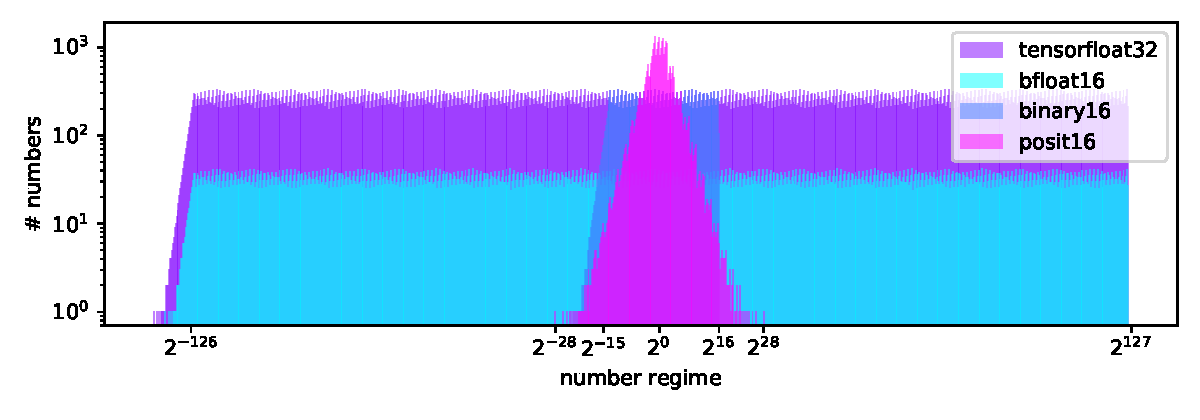
\includegraphics[width=1.0\textwidth]{plots/number_line2}
    \caption{Density and distribution of numbers for \gls{tensorfloat32}, \gls{binary16}, \gls{posit16} and \gls{bfloat16}. The number of bins was chosen to be \num{1024} of logarithmic width. The y-axis gives the amount of numbers in the number regime given by the x-axis. The IEEE conformant floats \gls{tensorfloat32}, \gls{binary16} and \gls{bfloat16} show a similar shape, namely the distribution of numbers is exponentially decreasing for higher and smaller numbers. The high numbers undergo a rough cut-off at the highest representable number. Numbers above that value will be cast to infinity. Compared to this, the small numbers show a smooth cut-off, because of the existence subnormal numbers. The range of \gls{posit16} is larger than the range of \gls{binary16}, but especially in their smallest numbers this difference in range is negligible. Some features of posits can be observed. First, their distribution is symmetric around \num{1}, because posits have no subnormals and the reciprocal of every number is in the set as well. Second, more numbers are closer to \num{1} than in case of floats; the closer to \num{1}, the better the number resolution. Closest to \num{1}, the number resolution becomes better than \gls{binary16} resolution. Third, posits have neither a fixed-length mantissa nor exponent. That is the reason the height of the posit shape depends on the number regime, which happens for floats only in the subnormal regime, where the exponent and mantissa are indeed of variable length. For all formats, the amount of numbers decreases exponentially when going away from \num{1}, but posits decrease faster. This suggests that when calculating in the number regime close to \num{1} posits might be the better choice, but when numbers span the entire number range equally, floats might be superior. In the latter case one has to take care about over- and underflows. Notice that the height of the shape is determined by the number of mantissa bits, therefore giving the precision, while the width is determined by the number of exponent bits, therefore giving the number range. For example, \gls{tensorfloat32} and \gls{binary16} have a vastly different number range but show the same precision for numbers in their intersection, meaning that \gls{binary16} is a subset of \gls{tensorfloat32}. On the other hand, \gls{tensorfloat32} and \gls{bfloat16} have approximately the same number range, but different precisions in them, meaning that \gls{bfloat16} is a subset of \gls{tensorfloat32}, which itself is a subset of \gls{binary32}. Notice that when plotting \gls{binary32} and \gls{posit32} in such a plot, they would look similar to \gls{binary16} vs. \gls{posit16}.}
    \label{fig:number_line}
\end{figure}

\subsection{Floating-point numbers in openQ*D}

To explore how the conjugate gradient kernel in openQ*D would perform when using smaller bit lengths, one can look at the exponential of the numbers in the matrix and vectors, see figure \ref{fig:exponents}. The plot shows all exponents appearing together with their overall occurrence in percent. The number zero was taken out of the plot, because it has biased exponent $E=-127$. The occurrences for zero are given in the legend.

The highest exponent in all 4 runs was $E=4$, while the lowest exponent decreased when the number of lattice points increased. The range of exponents that is representable in \gls{binary16} spans from \textcolor{corange}{$-24$} to \textcolor{cpink}{$+16$} and is indicated by the \textcolor{corange}{solid orange line} and the \textcolor{cpink}{solid pink line}. Between \textcolor{corange}{$-24$} and \textcolor{cblue}{$-14$} is the regime of subnormal numbers in \gls{binary16}, with the lowest regular (non-subnormal) exponent indicated by the \textcolor{cblue}{solid blue line}. When using half precision instead of single precision, all numbers with exponents below \textcolor{corange}{$-24$}, will be converted to zero, while exponents above \textcolor{cpink}{$+16$} will be cast to $\pm \infty$ depending on the sign of the number. It can be seen, that when calculating the norm of these numbers, only numbers between the \textcolor{cblue}{dashed blue line} and the \textcolor{cpink}{dashed pink line} will participate. If there is a number above the dashed pink line in the \textcolor{cyellow}{unsafe region} this number will -- after squaring -- be cast to $\infty$ and therefore the norm will be $\infty$ as well\footnotemark. In this case the variable holding the norm $x = \norm{\vec{v}}$ should be of higher precision than \gls{binary16}. The plot shows that the Dirac matrix \code{Dop()} is confined in a narrow exponent regime and a representation in 16-bit floats would suffice. Notice the sparsity of the Dirac matrix.

\footnotetext{A method to circumvent this is to scale the vector entries during the calculation and scale the result back, exploiting homogeneity of the norm, $\norm{\vec{v}} = \frac{1}{s}\norm{s\vec{v}}$ for $s \in \mathbb R_{> 0}$.}

\begin{figure}
    \centering
    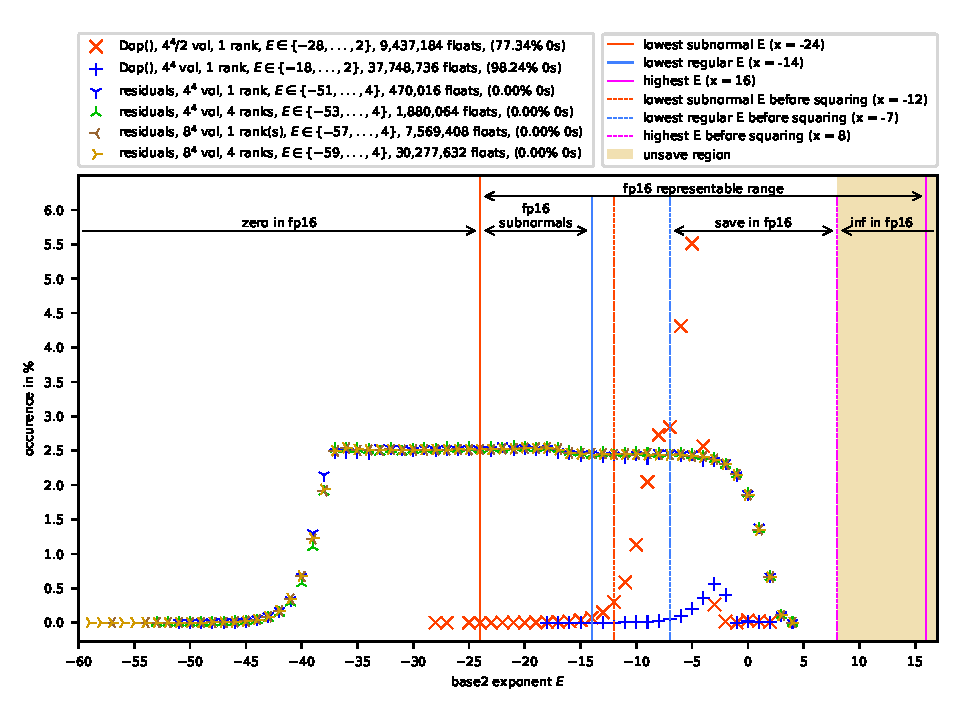
\includegraphics[width=1.0\textwidth]{plots/exponents_dirac}
    \caption{Exponent distribution of \gls{binary32} single precision floats in the residual vectors of all steps in a conjugate gradient run in openQ*D as well as entries of the Dirac-operator. 4 runs were made, with local lattice size of $4^4$ and $8^4$ on one single rank and $4$ ranks, respectively. The number is normalised to $(-1)^s \cdot M \cdot 2^{E}$, where $M \in [1, 2)$. For the Dirac-operator with volume $4^4/2$ only the even lattice points were considered.}
    \label{fig:exponents}
\end{figure}


\section{Conjugate Gradient}

\label{sec:cg}

Systems of linear equations need to be solved in many scientific computations. Usually, these systems are large, and the matrices and vectors are distributed among many \glspl{rank}. The method to solve such systems should therefore be iterative. The problem can be formulated mathematically in the following way.

\subsection{Derivation}

Let $n \in \mathbb{N}$ and $A$ be an $n \times n$-matrix with components in $\mathbb{C}$, Hermitian, positive definite and \glslink{sparse matrix}{sparse},

\begin{align*}
    A^{\dagger} &= A, &\text{(\df{Hermitian})} \\
    \forall \vec{x} \in \mathbb{C}^n \setminus \{0\} \quad \colon \quad \vec{x}^{\dagger} A \vec{x} &> 0, &\text{(\df{positive definite})}
\end{align*}

as well as $\vec{b} \in \mathbb{C}^n$ be given, then the \df{system of linear equations} can be described as

\begin{align}
    A \vec{x} = \vec{b}. \label{eq:Axb}
\end{align}

We are interested in the \df{solution} vector $\vec{x}$, that is the one that satisfies the above equation, $n$ is called the \df{problem size}. First let us define a function that will be helpful in the next sections.

\begin{definition}[Quadratic form]

The \df{quadratic form} depends on the problem matrix $A$ as well as on the \df{source} vector $\vec{b}$ and is defined as

\begin{align*}
    f(\vec{x}) = \frac{1}{2} \vec{x}^{\dagger} A \vec{x} - \vec{b}^{\dagger} \vec{x} + c,
\end{align*}

where $c \in \mathbb{C}$ (see figure \ref{fig:qform}).

\end{definition}

When taking the derivative of this function with respect to $\vec{x}$, we find that

\begin{align*}
    f'(\vec{x}) = A \vec{x} - \vec{b}.
\end{align*}

Therefore, finding the extrema of $f(\vec{x})$ is equivalent to solving the linear system of equations \eqref{eq:Axb}. The question whether the solution $\vec{x}$ is unique remains.

\begin{figure}
    \centering
    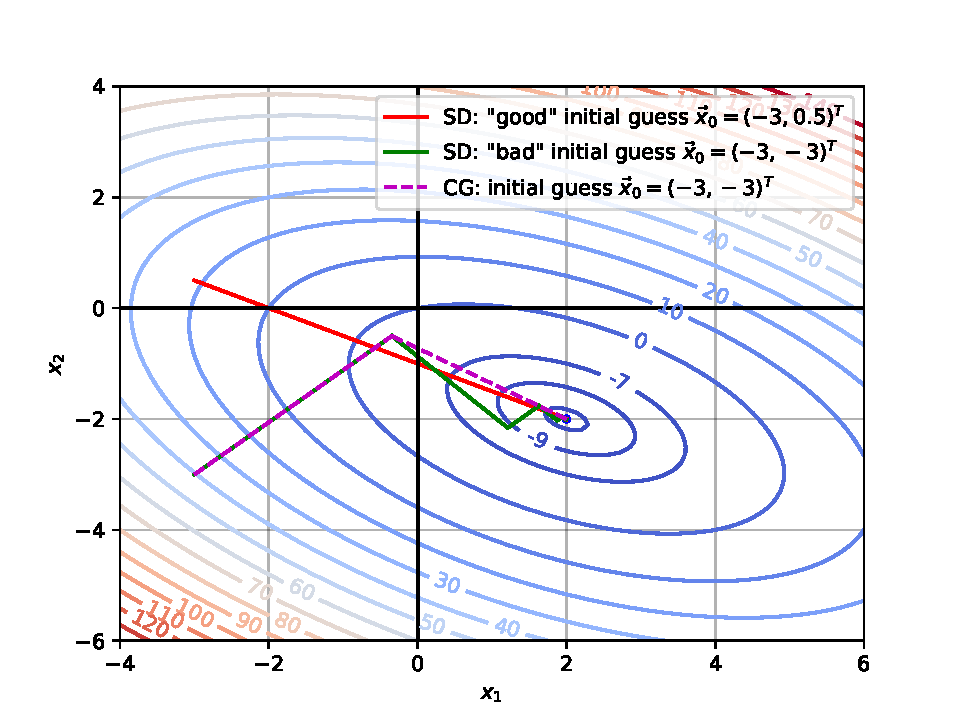
\includegraphics[width=0.7\textwidth]{plots/qform_contour2}
    \caption{Example of a quadratic form $f(\vec{x})$ with $A = \begin{pmatrix}
        3 & 2 \\
        2 & 6
    \end{pmatrix}$, $\vec{b} = (2, -8)^T$ and $c=0$. The analytic minimum is $\vec{x}^{*} = (2, -2)^T$. The red and green lines show two runs of steepest descent, with different starting vectors $\vec{x}_0$. The dashed magenta line shows a conjugate gradient run (notice that it only needed \num{2} steps).}
    \label{fig:qform}
\end{figure}

\begin{lemma}[Uniqueness of the solution]
The solution $\vec{x}$ in equation \eqref{eq:Axb} is unique and the global minimum of $f(\vec{x})$ if $A$ is Hermitian and positive definite \footnotemark.
\end{lemma}

\footnotetext{Negative definiteness is sufficient as well and $\vec{x}$ would be the global maximum instead -- define $A^{\prime} = -A$ which is positive definite and all the argumentation that follows will hold as well. Indefinite matrices on the other hand might have local minima and maxima.}

\begin{proof}
Let us rewrite $f(\vec{p})$ at an arbitrary point $\vec{p} \in \mathbb{C}$ in terms of the solution vector $\vec{x}$:

\begin{align*}
    f(\vec{p}) = f(\vec{x}) + \frac{1}{2} (\vec{p} - \vec{x})^{\dagger} A (\vec{p} - \vec{x}). \numberthis \label{eq:fp_cgne}
\end{align*}

This is indeed the same as $f(\vec{p})$ (inserting $A \vec{x} = \vec{b}$ and using $A^{\dagger}=A$ and $\vec{a}^{\dagger} \vec{b} = \vec{b}^{\dagger} \vec{a}$),

\begin{align*}
f(\vec{x}) + \frac{1}{2} (\vec{p} - \vec{x})^{\dagger} A (\vec{p} - \vec{x}) &= \frac{1}{2} \vec{x}^{\dagger} A \vec{x} - \vec{b}^{\dagger} \vec{x} + c + \frac{1}{2} \vec{p}^{\dagger} A \vec{p} - \frac{1}{2} \vec{p}^{\dagger} A \vec{x} - \frac{1}{2} \vec{x}^{\dagger} A \vec{p} + \frac{1}{2} \vec{x}^{\dagger} A \vec{x} \\
&= \frac{1}{2} \vec{p}^{\dagger} A \vec{p} + c + \vec{x}^{\dagger} \vec{b} - \vec{b}^{\dagger} \vec{x} - \vec{b}^{\dagger} \vec{p} \\
&= \frac{1}{2} \vec{p}^{\dagger} A \vec{p} - \vec{b}^{\dagger} \vec{p} + c \\
&= f(\vec{p}).
\end{align*}

In the new form of $f(\vec{p})$, one can directly see that if $A$ is positive definite, $\vec{x}$ must minimise the function:

\begin{align*}
    f(\vec{p}) = f(\vec{x}) + \frac{1}{2} \underbrace{ (\vec{p} - \vec{x})^{\dagger} A (\vec{p} - \vec{x}) }_{\text{$> 0$ if $A$ pos. def.}}.
\end{align*}

Therefore $\vec{x}$ is the global unique minimum.

\end{proof}

Before deriving the conjugate gradient method, we look at a related method called the \df{method of steepest descent}. We are interested in a method that iteratively solves equation \eqref{eq:Axb} starting at a \df{initial guess} $\vec{x}_0$ until the series is interrupted, because the approximate solution $\vec{x}_i$ might be close to the real solution by a certain tolerance or the solution was found exactly,

\begin{align*}
    \vec{x}_0 \longrightarrow \vec{x}_1 \longrightarrow \dotsb \longrightarrow \vec{x}_i \longrightarrow \vec{x}_{i+1} \longrightarrow \dotsb
\end{align*}

For each step, we can define the \df{error} and \df{residual} of the current step $i$.

\begin{definition}[Error and residual]

Define the \df{error} $\vec{e}_i$ and the \df{residual} $\vec{r}_i$ as

\begin{subequations}
    \begin{align}
        \vec{e}_i &= \vec{x}_i - \vec{x}, \label{eq:error} \\
        \vec{r}_i &= \vec{b} - A \vec{x}_i. \label{eq:residual}
    \end{align}
\end{subequations}

\end{definition}

The residual is the vector of discrepancies and the same as $\vec{r}_i = -f'(\vec{x}_i) = -A \vec{e}_i$, the negative derivative of the quadratic form. The derivative points in direction of the maximal increase, thus the residual points in direction of the steepest descent seen from the position of point $\vec{x}_i$.

\begin{definition}[Method of Steepest Descent (SD)]
The iteration step equation of the \df{method of steepest descent} in defined as

\begin{align}
    \vec{x}_{i+1} = \vec{x}_i + \alpha_i \vec{r}_i \label{eq:steepest_descent},
\end{align}

where the $\alpha_i \in \mathbb{C}$ are the amounts to go in direction of the current residual $\vec{r}_i$. The $\alpha_i$ are determined by minimising the parabola with respect to $\alpha_i$, $\frac{d}{d \alpha_i} f(\vec{x}_{i+1}) \stackrel{!}{=} 0$.

\end{definition}

\begin{remark}[Convergence]
The method of steepest descent converges very slowly to the actual solution, when starting at an unfavourable starting point $\vec{x}_0$ (see figure \ref{fig:qform}). The speed of convergence heavily depends on the condition number of the matrix $A$. The process happens to go in the same direction multiple times. If we only go one step in each direction $i$ by the perfect amount $\alpha_i$, we would be done after at most $n$ steps.
\end{remark}

This gives motivation for an enhanced method. Let's define a new \df{step equation} as

\begin{align}
    \vec{x}_{i+1} = \vec{x}_i + \alpha_i \vec{p}_i, \label{eq:cg_step}
\end{align}

with \df{directions} $\vec{p}_i$ and \df{amounts} $\alpha_i$ which we have to determine. But this time, we will impose the condition to go in every direction only once at most. This will lead us to the \df{method of conjugate gradient}.

Using the step equation \eqref{eq:cg_step}, we can update the error and residuals,

\begin{subequations}
    \begin{align}
        \vec{e}_{i+1} &= \vec{x}_{i+1} - \vec{x} \\
                      &= \vec{e}_{i} + \alpha_i \vec{p}_{i} \label{eq:cg_error1} \\
                      &= \vec{e}_{0} + \sum_{j=0}^{i} \alpha_j \vec{p}_{j}, \label{eq:cg_error2}
    \end{align}
\end{subequations}

\begin{subequations}
    \begin{align}
        \vec{r}_{i+1} &= \vec{b} - A \vec{x}_{i+1} \label{eq:residual_exact} \\
                      &= \vec{r}_{i} - \alpha_i A \vec{p}_{i} \label{eq:residual_recursive} \\
                      &= - A \vec{e}_{i+1}. \label{eq:residual_exact2}
    \end{align}
\end{subequations}

The $\{\vec{p}_i\}$ need to form a basis of $\mathbb{C}^n$, because the method should succeed with any arbitrary initial guess $\vec{x}_0$. Since we move in the vector space $\mathbb{C}^n$ from an arbitrary point $\vec{x}_0$ to the solution $\vec{x}$, the $n$ direction vectors need to cover all possible directions in the space, therefore need to be linear independent.

To be done after at most $n$ steps, we require the $n$-th error to be zero, $\vec{e}_n = 0$. Since the directions form a basis, we can write $\vec{e}_0$ as a linear combination of the $\{\vec{p}_i\}$,

\begin{align*}
    \vec{e}_{0} = \sum_{j=0}^{n-1} \delta_j \vec{p}_j.
\end{align*}

Using this we can rewrite $\vec{e}_n$,

\begin{align*}
    \vec{e}_{n} &= \vec{e}_o + \sum_{j=0}^{n-1} \alpha_j \vec{p}_j \\
                &= \sum_{j=0}^{n-1} \delta_j \vec{p}_j + \sum_{j=0}^{n-1} \alpha_j \vec{p}_j \\
                &= \sum_{j=0}^{n-1} (\delta_j + \alpha_j) \vec{p}_j.
\end{align*}

For this to be zero, all coefficients need to be zero, thus $\delta_j = - \alpha_j$. Then the $i$-th error can be rewritten as

\begin{align*}
    \vec{e}_{i} &= \vec{e}_0 + \sum_{j=0}^{i-1} \alpha_j \vec{p}_j \\
                &= \sum_{j=0}^{n-1} \delta_j \vec{p}_j - \sum_{j=0}^{i-1} \delta_j \vec{p}_j \\
                &= \sum_{j=i}^{n-1} \delta_j \vec{p}_j. \numberthis \label{eq:error_i}
\end{align*}

In the last row, we can see that after every step in the iteration, we shave off the contribution of one direction $\vec{p}_i$ to the initial error $\vec{e}_0$ (or equivalent: $\vec{e}_{i+1}$ has no contribution from previous directions $\vec{p}_i, \vec{p}_{i-1}, \dots$). We still need to find these directions. We could for example impose that the $(i+1)$-th error should be orthogonal to the $i$-th direction, because we never want to go in that direction again,

\begin{align*}
    0 &\stackrel{!}{=} \vec{p}_i^{\dagger} \vec{e}_{i+1} \\
                    &= \vec{p}_i^{\dagger} ( \vec{e}_{i} + \alpha_i \vec{p}_i ).
\end{align*}

This gives us an expression for the amount $\alpha_i$,

\begin{align*}
    \alpha_i = - \frac{ \vec{p}_i^{\dagger} \vec{e}_{i} }{ \vec{p}_i^{\dagger} \vec{p}_i }.
\end{align*}

The problem with this expression is that we don't know the value of $\vec{e}_i$ -- if we would, we could subtract it from the current $\vec{x}_i$ and obtain $\vec{x}$ exactly. We do not know $\vec{e}_i$, but what we know is something similar, namely $-A \vec{e}_i$, with is the residual. If we manage to insert an $A$ in the expression above, we reached the goal. It turns out that imposing $A$-orthogonality instead of regular orthogonality between $\vec{e}_{i+1}$ and $\vec{p}_i$ accomplishes the desired result\footnotemark,

\begin{align*}
    0 &\stackrel{!}{=} \vec{p}_i^{\dagger} A \vec{e}_{i+1} \\
                    &= \vec{p}_i^{\dagger} A ( \vec{e}_{i} + \alpha_i \vec{p}_i ). \\
\end{align*}

\footnotetext{This is equivalent to imposing $0 \stackrel{!}{=} \vec{r}_{i+1}^{\dagger} \vec{p}_i$ which is done in most literature, but in the opinion of the author this is less intuitive.}

Solving for $\alpha_i$ gives the (almost) final expression for the amounts,

\begin{align}
      \implies         \alpha_i &= - \frac{ \vec{p}_i^{\dagger} A \vec{e}_{i} }{ \vec{p}_i^{\dagger} A \vec{p}_i } = \frac{ \vec{p}_i^{\dagger} \vec{r}_{i} }{ \vec{p}_i^{\dagger} A \vec{p}_i }. \label{eq:cgne:alpha_pre}
\end{align}

Notice that the denominator is never zero, because $A$ is positive definite. Let us continue with the expression for $A$-orthogonality, but insert the derived expression \eqref{eq:error_i} for $\vec{e}_{i+1}$ this time,

\begin{align*}
    0 &\stackrel{!}{=} \vec{p}_i^{\dagger} A \vec{e}_{i+1} \\
                    &= \vec{p}_i^{\dagger} A \left[ \sum_{j=i+1}^{n-1} \delta_j \vec{p}_j \right] \\
                    &= \sum_{j=i+1}^{n-1} \underbrace{ \delta_j }_{\text{\makebox[0pt]{$\neq 0$} }} \vec{p}_i^{\dagger} A \vec{p}_j.
\end{align*}

This implies that for $j>i$ and $i \in \{0, \dots, n-1\}$, we have

\begin{align*}
    \vec{p}_i^{\dagger} A \vec{p}_j = 0.
\end{align*}

But since $A$ is Hermitian, we can Hermitian conjugate the entire expression above and obtain

\begin{align*}
    0 = \left( \vec{p}_i^{\dagger} A \vec{p}_j \right)^{\dagger} = \vec{p}_j^{\dagger} A \vec{p}_i.
\end{align*}

So the expression holds for $i>j$ as well, which implies that the $\{\vec{p}_i\}$ are \df{$A$-orthogonal},

\begin{align*}
    \vec{p}_i^{\dagger} A \vec{p}_j = 0 \quad \forall i \neq j.
\end{align*}

The problem has reduced to finding a set of $A$-orthogonal vectors in an iterative way. Luckily, there is a well know method to find orthogonal vectors from a set of linear independent vectors: \df{Gram-Schmidt orthogonalization}. The procedure can be altered to find $A$-orthogonal vectors instead.

\begin{definition}[Gram-Schmidt Orthogonalization]

\label{df:gramschmidt}

Let $\{ \vec{u}_0, \dots, \vec{u}_{n-1} \} \subset \mathbb{C}^n$ be a set of $n$ linear independent vectors. The iterative Gram-Schmidt procedure is

\begin{align}
    \begin{split}
        \vec{p}_0 &= \vec{u}_0 \label{eq:gramschmidt} \\
        \vec{p}_i &= \vec{u}_i + \sum_{k=0}^{i-1} \beta_{ik} \vec{p}_k,
    \end{split}
\end{align}

where the $\beta_{ik} \in \mathbb{C}$ are coefficients (to be determined).

\end{definition}

In the regular procedure, the $\beta_{ik}$ are normalised projections of $\vec{u}_i$ to $\vec{p}_k$ that are subtracted from $\vec{u}_i$, leading to a vector $\vec{p}_i$ that is orthogonal to all previously calculated $\vec{p}_k$. In our problem, we need a set of vectors that are $A$-orthogonal. By imposing this condition, we find a different expression for the $\beta_{ik}$,

\begin{align*}
    0 &\stackrel{!}{=} \vec{p}_i^{\dagger} A \vec{p}_j \\
                    &= \vec{u}_i^{\dagger} A \vec{p}_j + \sum_{k=0}^{i-1} \beta_{ik} \vec{p}_k^{\dagger} A \vec{p}_j \\
                    &= \vec{u}_i^{\dagger} A \vec{p}_j + \beta_{ij} \vec{p}_j^{\dagger} A \vec{p}_j,
\end{align*}

where in the last step, we assumed $i>j$ (else we would not find an expression for $\beta_{ij}$) and therefore only the $j$-th term in the sum remains, because of the $A$-orthonormality of the directions. Solving this for $\beta_{ij}$ gives

\begin{align}
    \beta{ij} = - \frac{ \vec{u}_i^{\dagger} A \vec{p}_j }{ \vec{p}_j^{\dagger} A \vec{p}_j }. \label{eq:betas}
\end{align}

In principle we are done here, we only need a set of linearly independent vectors $\{\vec{u}_i\}$. Since the conjugate gradient method is iterative and often dealing with huge problem sizes $n$, we need to store all previous directions $\vec{p}_k$ in order to calculate the current direction (see equation \eqref{eq:gramschmidt}). This becomes a problem in limited memory situations. We want that the current step only depends on the previous one. By imposing this condition, we need the sum in equation \eqref{eq:gramschmidt} to collapse; the $\beta_{ik}$ should only be non-zero for $k=i-1$. If we manage to satisfy this, the orthogonalization procedure would simplify to

\begin{align*}
    \beta_i &\coloneqq \beta_{i, i-1}, \\
    \vec{p}_i &= \vec{u}_i + \beta_i \vec{p}_{i-1},
\end{align*}

where in the second equation, the current $\vec{p}_i$ only depends on the previous $\vec{p}_{i-1}$. For this to hold, all other $\beta_{ij}$ need to be zero. For such a $\beta_{ij}$ the numerator needs to be zero. Let therefore $j<i-1$

\begin{align*}
    \vec{u}_i^{\dagger} A \vec{p}_j &\stackrel{!}{=} 0.
\end{align*}

To find a different expression for the left-hand side, consider

\begin{align*}
    \vec{u}_i^{\dagger} \vec{r}_{j+1} &= \vec{u}_i^{\dagger} \left( \vec{r}_j - \alpha_j A \vec{p}_j \right) \\
    &= \vec{u}_i^{\dagger} \vec{r}_j - \alpha_j \textcolor{cyellow}{\vec{u}_i^{\dagger} A \vec{p}_j}, \\
    \implies \textcolor{cyellow}{\vec{u}_i^{\dagger} A \vec{p}_j} &= \frac{1}{\alpha_j} \left[ \vec{u}_i^{\dagger} \vec{r}_j - \vec{u}_i^{\dagger} \vec{r}_{j+1} \right], \numberthis \label{eq:uiAdj}
\end{align*}

where we inserted the recursive relation of the residuals \eqref{eq:residual_recursive} and the \textcolor{cyellow}{yellow} part is the expression we want to be \textcolor{cyellow}{zero} for $j<i-1$. We therefore find a condition for the linear independent set $\{\vec{u}_i\}$, namely that the scalar product of $\vec{u}_i$ with $\vec{r}_{j+1}$ and $\vec{r}_{j}$ must be the same. We can apply the same equation multiple times and obtain for $j<i-1$

\begin{align*}
    \vec{u}_i^{\dagger} \vec{r}_{j+1} &= \vec{u}_i^{\dagger} \vec{r}_j = \dots = \vec{u}_i^{\dagger} \vec{r}_0.
\end{align*}

We have to find $\{\vec{u}_i\}$ that satisfy the above equation. It is sufficient to find a set of $\{\vec{u}_i\}$ that are orthogonal to all the residuals in order for the equation to be obeyed.

\begin{lemma}[]
\label{lem:rorthogonality}
The residuals are orthogonal, thus for all $i \neq j$, it holds

\begin{align*}
    \vec{r}_i^{\dagger} \vec{r}_j = 0.
\end{align*}

\end{lemma}

\begin{proof}

The proof consists of 2 steps.

\begin{enumerate}[label={\arabic*)}]
    \item Let $i<j$,

    \begin{align*}
        \vec{p}_i^{\dagger} \vec{r}_j &= - \vec{p}_i^{\dagger} A \vec{e}_j \\
                                      &= - \sum_{k=j}^{n-1} \delta_j \textcolor{cyellow}{\vec{p}_i A \vec{p}_k} \\
                                      &= 0,
    \end{align*}

    where the \textcolor{cyellow}{yellow} expression is \textcolor{cyellow}{zero}, because $i<j\leq k$.

    \item Let $i<j$. By step 1), we have

    \begin{align*}
        0 &= \vec{p}_i^{\dagger} \vec{r}_j \\
          &= \vec{r}_i^{\dagger} \vec{r}_j + \sum_{k=0}^{i-1} \beta_{ik} \textcolor{cyellow}{\vec{p}_k^{\dagger} \vec{r}_j} \\
          &= \vec{r}_i^{\dagger} \vec{r}_j.
    \end{align*}

    The \textcolor{cyellow}{yellow} expression is again \textcolor{cyellow}{zero} by step 1). Using the symmetry of the scalar product, the above equation holds for $i$ and $j$ interchanged ($i>j$) too, therefore holds for all $i \neq j$.

\end{enumerate}

\end{proof}

In the following, we set $\vec{u}_i = \vec{r}_i$. What remains to find is the final expression for the $\beta_i$.

\begin{align*}
    \beta_i \coloneqq \beta_{i,i-1} &= - \frac{ \vec{u}_i^{\dagger} A \vec{p}_{i-1} }{ \vec{p}_{i-1}^{\dagger} A \vec{p}_{i-1} } \\
    &= - \frac{1}{\vec{p}_{i-1}^{\dagger} A \vec{p}_{i-1} } \frac{1}{\alpha_{i-1}} \left[ \textcolor{cyellow}{\vec{r}_i^{\dagger} \vec{r}_{i-1}} - \vec{r}_i^{\dagger} \vec{r}_i \right] \\
    &= \frac{ \vec{r}_i^{\dagger} \vec{r}_i }{ \alpha_{i-1} \vec{p}_{i-1}^{\dagger} A \vec{p}_{i-1} } \\
    &= \frac{ \vec{r}_i^{\dagger} \vec{r}_i }{ \vec{p}_{i-1}^{\dagger} \vec{r}_{i-1} },
\end{align*}


where in the first row we used the definition \eqref{eq:betas}, in the second row we have used equation \eqref{eq:uiAdj} and the \textcolor{cyellow}{yellow} expression is \textcolor{cyellow}{zero} by the orthogonality of the residuals, lemma \ref{lem:rorthogonality}. In the last line we used the expression for the $\alpha_j$ equation \eqref{eq:cgne:alpha_pre}.

To obtain the final form of the $\alpha_i$ and the $\beta_i$, we can use the proof of lemma \ref{lem:rorthogonality}, namely

\begin{align*}
    \vec{p}_i^{\dagger} \vec{r}_i &= \vec{r}_i^{\dagger} \vec{r}_i + \beta_i \underbrace{\textcolor{cyellow}{\vec{p}_{i-1}^{\dagger} \vec{r}_i}}_{ \mathrlap{\text{$=0$ by lemma \ref{lem:rorthogonality} step 1) }} } \\
    &= \vec{r}_i^{\dagger} \vec{r}_i.
\end{align*}


Using this we find the final form of the $\alpha_i$ and the $\beta_i$ as well as the \df{method of conjugate gradient}.

\begin{definition}[Method of conjugate gradient (CG)]

\label{def:cg}

The iteration step equation of the \df{method of conjugate gradient} in defined as

\begin{align*}
    \vec{x}_{i+1} = \vec{x}_i + \alpha_i \vec{p}_i,
\end{align*}

with

\noindent\begin{minipage}{.5\linewidth}
    \begin{align*}
        \vec{r}_{i+1} &= \vec{r}_{i}   - \alpha_i A  \vec{p}_i, \\
        \vec{p}_{i+1} &= \vec{r}_{i+1} + \beta_{i+1} \vec{p}_i, 
    \end{align*}
\end{minipage}
\begin{minipage}{.5\linewidth}
    \begin{align}
        \alpha_i    &= \frac{ \vec{r}_{i}^{\dagger} \vec{r}_{i} }{ \vec{p}_i^{\dagger} A \vec{p}_i }, \label{eq:alphai} \\
        \beta_{i+1} &= \frac{ \vec{r}_{i+1}^{\dagger} \vec{r}_{i+1} }{ \vec{r}_{i}^{\dagger} \vec{r}_{i} }, \label{eq:betai}
    \end{align}
\end{minipage}

and initial starting vectors

\begin{align*}
    \vec{x}_{0} &= \text{arbitrary starting point}, \numberthis \label{eq:cg:start} \\
    \vec{p}_{0} &= \vec{r}_{0} = \vec{b} - A \vec{x}_0.
\end{align*}

\end{definition}

There are some remarks to note about the method of conjugate gradient.

\begin{remark}
    The $\beta_{i+1}$ of the current iteration depends on the norm of the current residual as well as the last one. This means that we can store the result of the last iteration and reuse it in the current, the norm may not be calculated twice.
\end{remark}

\begin{remark}
    In the source code of openQ*D (see \cite{openqxd}) the matrix $A$ is the Dirac matrix applied twice $A = D^{\dagger} D$. This means that the denominator of $\alpha_i$ is a regular inner product as well; $\vec{p}_i^{\dagger} A \vec{p}_i = \vec{p}_i^{\dagger} D^{\dagger} D \vec{p}_i = \left( D \vec{p}_i \right)^{\dagger} \left( D \vec{p}_i \right) = \norm{ D \vec{p}_i }^2$.
\end{remark}

\begin{remark}
    Therefore in each iteration, we have:
    \begin{itemize}
        \item 2 times the norm of a vector,
        \item 2 matrix-vector multiplications,
        \item 3 times axpy.\footnotemark
    \end{itemize}
\end{remark}

\footnotetext{This stands for $a \vec{x} + \vec{y}$, scalar times vector plus vector, "a x plus y" (to resemble the \acrshort{BLAS} level 1 routine call of the same name).}

\begin{remark}[Floating-point errors]
    Since the method introduces recursive steps, floating-point round-off accumulation has to be dealt with. This causes the residuals to lose their $A$-orthogonality. It can be resolved by calculating the residual from time to time using its (computationally more expensive) definition $\vec{r}_i = \vec{b} - A \vec{x}_i$, which involves one matrix vector multiplication (or two is $A=D^{\dagger}D$). One can for example do this every $m$-th step. The same problem applies to the directions $\vec{p}_i$ that lose their $A$-orthogonality.
\end{remark}

\begin{remark}[Problem size]
    The method of conjugate gradient is suitable for problems of enormous sizes $n$. The algorithm is done after $n$ steps (see figure \ref{fig:qform}), but there might be problems such that even $n$ steps are out of reach for an exact solution.
\end{remark}

\begin{remark}[Complexity]
    The time complexity of the conjugate gradient method is $O(m \sqrt{\kappa})$, where $m$ is the number of non-zero entries in $A$ and $\kappa$ is its \df{condition number}. The space complexity is $O(m)$.
\end{remark}

\begin{remark}[Starting]
    The \df{starting vector} $\vec{x}_0$ can be chosen arbitrarily. If there is already a rough estimate of the solution one can take that vector. Usually, $\vec{x}_0 = 0$ is chosen. Since the minimum is global, there is no issue in choosing a starting point. The method will always converge towards the real solution.
\end{remark}

\begin{remark}[Stopping]
    If the problem size does not allow to run $n$ steps, one can stop when the norm of the residual falls below a certain \df{threshold} $\epsilon$. Usually, this threshold is a fraction of the initial residual $\norm{\vec{r}_i} < \epsilon \norm{\vec{r}_0}$, \cite{shewchuk1994}.
\end{remark}

\begin{remark}[Initialisation]
    The very first step of the method is equivalent to a step in the method of steepest descent, see equation \eqref{eq:steepest_descent} as well as figure \ref{fig:qform}.
\end{remark}

\begin{remark}[Speed of convergence]
    Conjugate gradient is faster if there are duplicated eigenvalues. The number of iterations for an exact solution is at most the number of distinct eigenvalues.
\end{remark}

\begin{remark}[Preconditioning]
    The linear system of equations can be transformed using a matrix $M$ to

    \begin{align*}
        M^{-1} A \vec{x} = M^{-1} \vec{b}.
    \end{align*}

    It is assumed $M$ is such that it is easy to invert, and it approximates $A$ in some way, resulting in $M^{-1} A$ to be better conditioned than $A$\footnote{Or equivalent, $M^{-1}A$ has a more clustered spectrum than $A$.}. An example of a particular preconditioner $M$ is a diagonal matrix, with diagonal entries of $D$. It is indeed easy to invert, and it approximates $A$ quite well if $A$ has non-zero diagonal entries and most off-diagonal entries are zero.
\end{remark}

\begin{remark}[\acrfull{cgne}]
    The algorithm can be used even if $A$ is neither symmetric nor Hermitian nor positive definite. The linear system of equations to be solved is then

    \begin{align*}
        A^{\dagger} A \vec{x} = A^{\dagger} \vec{b}.
    \end{align*}

    If $A$ is square and invertible, solving the above equation is equivalent to solving $A \vec{x} = \vec{b}$. Conjugate gradient can be applied, because $A^{\dagger} A$ is Hermitian and positive definite ($\vec{x}^{\dagger} A^{\dagger} A \vec{x} = \norm{A \vec{x}} \ge 0$). Notice that $A^{\dagger} A$ is less sparse than $A$, and often $A^{\dagger} A$ is badly conditioned.

\end{remark}

\subsection{CG kernel in openQ*D}

\label{sec:fp_in_openqxd}

The conjugate gradient kernel \code{cgne()} in \code{modules/linsolv/cgne.c} in \cite{openqxd} implements the algorithm, see listing \ref{lst:cgne}. The algorithm is already implemented in mixed precision using \gls{binary32} in most of the computations and \gls{binary64} in correction steps\footnote{The method is also referred to as \df{mixed precision defect-correction}, see \cite{goddeke2005}}.

\begin{comment}
The disadvantage of defect-correction, however, is that the Krylov search space that is built up is discarded each time the solver is restarted.

Other possibility: "reliable updates" scheme:
\end{comment}

\begin{figure} % wrap into a figure such that the whole snippet is on the same page
\begin{lstlisting}[
    language=C,
    firstnumber=429,
    label=lst:cgne,
    caption={The conjugate gradient kernel in \code{modules/linsolv/cgne.c} line \num{429}ff. The volume of the lattice is given by \code{vol}, \code{icom} is a communication control parameter, \code{Dop()} and \code{Dop\_dble()} are the Dirac-operators in single and double-precision, \code{ws} and \code{wsd} are workspace allocations. The remaining parameters are the maximum number of iterations \code{nmx}, the relative residue \code{res}, the source spinor \code{eta}, the starting spinor, which also holds the result after the run \code{psi}. \code{status} holds the number of CG-steps performed. The return value is the norm of the residual of the current solution.}
]
double cgne(int vol,int icom,void (*Dop)(spinor *s,spinor *r),
            void (*Dop_dble)(spinor_dble *s,spinor_dble *r),
            spinor **ws,spinor_dble **wsd,int nmx,double res,
            spinor_dble *eta,spinor_dble *psi,int *status)
\end{lstlisting}
\end{figure} 

The function requires the Dirac-operator \code{Dop()} in \gls{binary32}, \code{Dop\_dble()} in \gls{binary64} format and the source vector \code{eta} ($\vec{b}$) in \gls{binary64} only. In the initialisation, the starting vector \code{psi} ($\vec{x}_0$) is set to zero. The algorithm stops when the desired maximal relative residue $\code{res} =\frac{\norm{\code{eta}-D^\dagger D \code{psi}}}{\norm{\code{eta}}}$ is reached, where \code{psi} is the calculated approximate solution of the Dirac equation $D^\dagger D \code{psi}=\code{eta}$ in \gls{binary64}. For this, the tolerance \code{tol} is calculated using $\code{tol} = \norm{\code{eta}} * \code{res}$. The parameter \code{nmx} is the maximal number of iterations that may be applied and \code{status} reports the total number of iterations that were needed, or a negative value if the algorithm failed. \code{icom} is a control parameter and \code{ws} and \code{wsd} are workspace allocations. The volume of the local lattice should be provided in \code{vol} when calling the function.

Since the Dirac-operator is given in two precisions, the algorithm in the code bails out of the main conjugate gradient loop, when some particular conditions are met, see listing \ref{lst:break}.

\begin{figure} % wrap into a figure such that the whole snippet is on the same page
\begin{lstlisting}[
    language=C,
    firstnumber=490,
    label=lst:break,
    caption={Break condition in \code{modules/linsolv/cgne.c} line \num{490}ff, \code{rn} is the norm of the current residual, \code{xn} is the norm of the current solution vector, both in \gls{binary32}. The other parameters are the tolerance \code{tol}, the current iteration number \code{status}, the current iteration number since the last restart step \code{ncg} and the maximal number of iterations \code{nmx}.}
]
if ((rn<=tol)||(rn<=(PRECISION_LIMIT*xn))||(ncg>=100)||
    ((*status)>=nmx))
   break;
\end{lstlisting}
\end{figure} 

This may happen in 4 cases:

\begin{enumerate}
  \item if the recursively calculated residual is below the tolerance,
  \item if the precision of \gls{binary32} is reached\footnotemark,
  \item after a hard coded number of \num{100} steps since the last restart step,
  \item if the maximal number of steps \code{nmx} is reached.
\end{enumerate}

\footnotetext{The constant \code{PRECISION\_LIMIT} is defined to be \code{100*MACHINE\_EPSILON}, where the \code{MACHINE\_EPSILON} is the difference between \num{1} and the lowest value above \num{1} depending on the data type. In case of \gls{binary32} the \code{MACHINE\_EPSILON} takes a value of \num[round-mode = figures, round-precision = 8, scientific-notation = true]{1.1920928955078125e-07}.}

We discuss in the following the second condition in more detail: assume the precision of \gls{binary32} is reached, but the algorithm does not break out of the main loop. Therefore, the norm of the current residual compared to the norm of the current solution vector differ in their orders of magnitude by the precision limit of their data type (\gls{binary32} in this case). This means that the solution vector $\vec{x_i}$ contains large numbers compared to the residual vector $\vec{r_i}$. Therefore, the changing in residual in successive iterations is negligible compared to numbers in $\vec{x_i}$ as well. Since $\vec{r_i}$ contains small numbers, the amounts $\alpha_i$ are small too. This causes $\vec{x_{i+1}} = \vec{x_i} + \alpha_i \vec{d_i}$ to not change anymore, because adding very large and very small numbers in floating-point arithmetic will return the larger number unchanged if the two numbers differ in magnitude by the precision limit of the data type. The algorithm stalls in that case and breaking out of the main loop is the emergency brake in such a case.

When one of the above conditions is met, the algorithm performs a \df{reset step} (or \df{restart step}). In a reset step, the residual is not calculated in the recursive way (as described above in definition \eqref{def:cg}) but by its definition $\vec{r_i} = \vec{b} - A \vec{x_i}$ in double precision. Such a step involves two invocations of each \code{Dop\_dble()} as well as \code{Dop()} which is expensive. The algorithm is resetting in the sense that the solution vector is set back to $\vec{x_i} = 0$, but before resetting, the solution vector in \gls{binary32} is added to the real solution vector \code{psi} in \gls{binary64} which was initialised to zero at the start of the algorithm. It looks like a restart of the entire calculation, but the direction for the next iteration $\vec{d_i} = \vec{r_i}$ is set to the just calculated, more accurate residual. Therefore, the algorithm now continues in a new direction $A$-orthogonal to all previous directions and progression is kept. The step is meant to remove the accumulated round-off errors due to the recursive calculation of the residuals and directions. The first step following a reset step is a step in the direction of steepest descent like the very first step of the algorithm. The less precise the data type, the more reset steps are required, because the precision limit (case 2) is reached earlier.

\subsection{Simulating CG with different data types}

\label{sec:simulating_cgne}

Some operations such as norms, scalar products and applications of the Dirac-operator are memory-bound, which means the memory bandwidth of the controller and main memory determine how much time is spent in performing the operation. Storing input data in a format with lower bit-length reduces the amount of data to be transferred from and to main memory, thus improving the speed of calculation.

\subsubsection{Setup}

The complete conjugate gradient kernel was simulated in different data types, floats as well as posits. To produce the plot series, the Dirac matrix \code{Dop\_dble()} and the source vector $\code{eta}$ were extracted in \gls{binary64} format from the original code running a simulation of a $4^4$ lattice, \acrfull{sf} boundary conditions (\code{type 1}), no C* boundary conditions (\code{cstar 0}) and $1$ rank. The first \num{2000} trajectories were considered thermalisation. The matrix was extracted in trajectory \num{2001}. A Python script mimicking the exact behaviour of the \code{cgne()} kernel from the source code, was implemented to cope with arbitrary data types. The simulated data types were \gls{binary64}, \gls{binary32}, \gls{tensorfloat32}, \gls{binary16}, \gls{bfloat16}, \gls{posit32}, \gls{posit16}, and \gls{posit8}. The considered Dirac-operator represented as a \acrshort{csr}-matrix had approximately \num{2}\% non-zero values. The results are plotted in figures \ref{fig:cgne:naive} - \ref{fig:cgne:res12}.

\begin{comment}
\begin{figure}
    \centering
    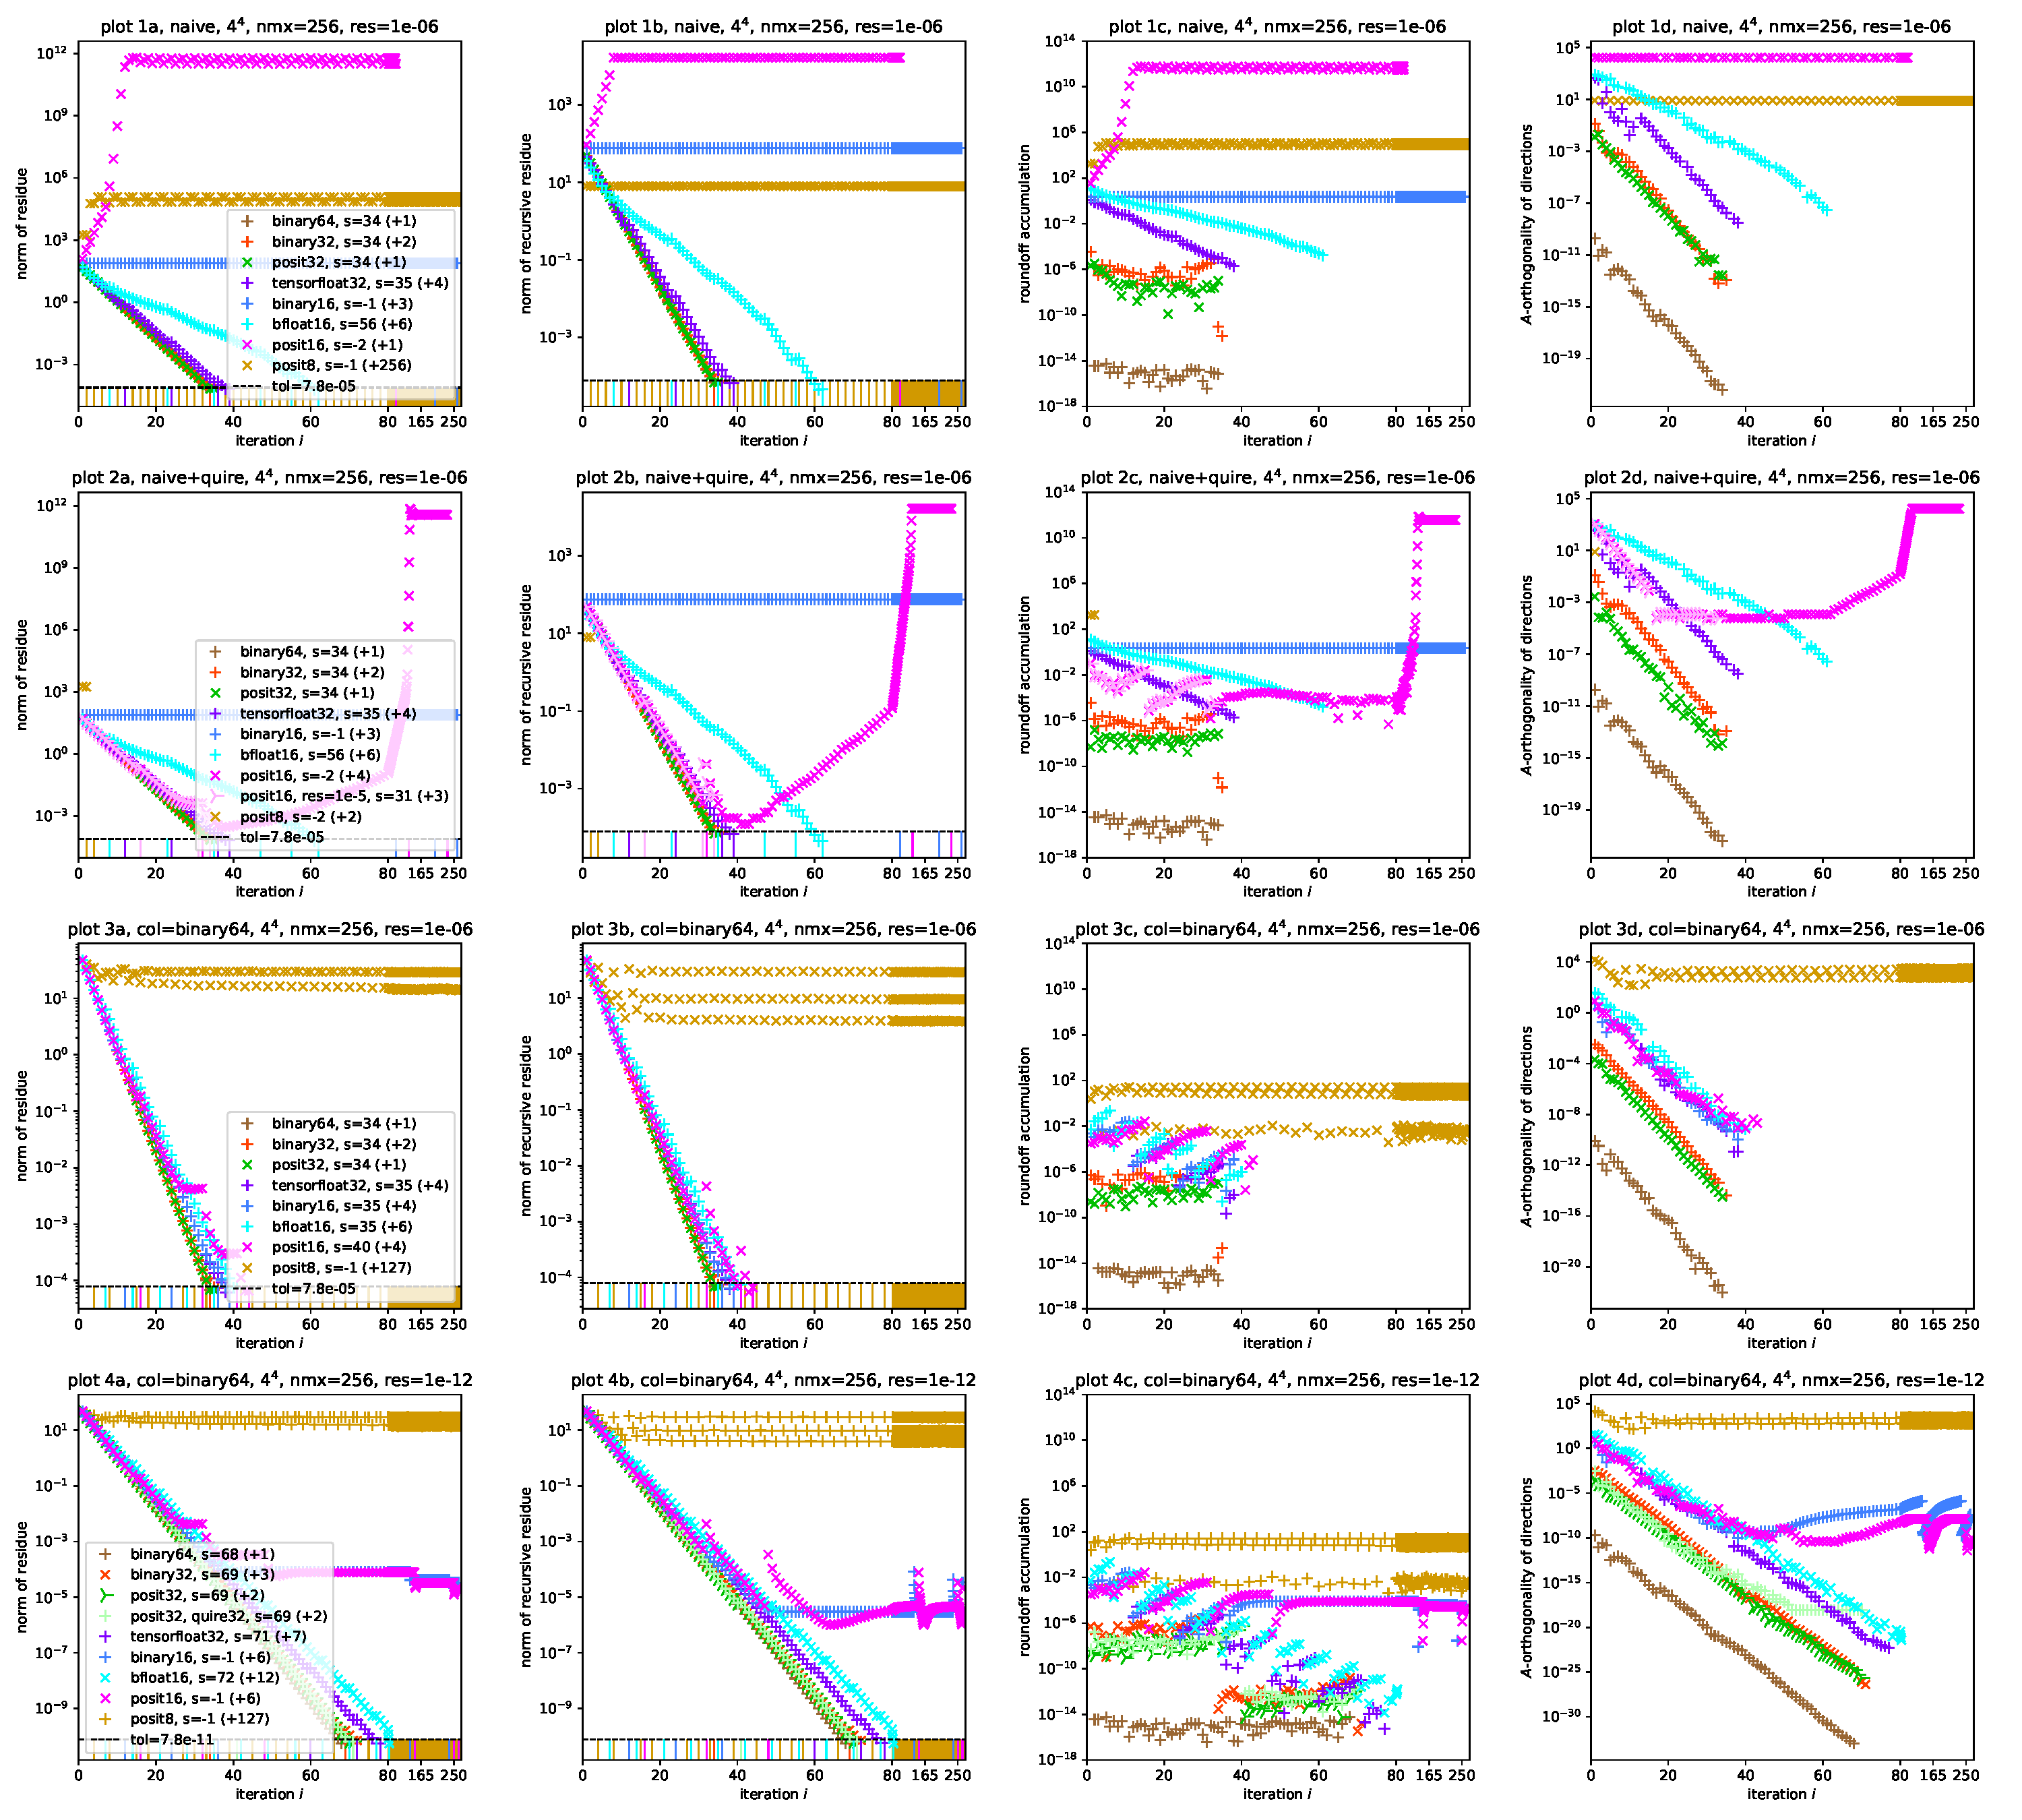
\includegraphics[width=1.0\textwidth]{plots/cgne}
    \caption{Convergence analysis of a conjugate gradient run, where \gls{binary32} was replaced by one of the simulated data types. The legend for every row is equal, displayed only in the first plot of the row. The number \code{s} describes the number of normal steps needed (the value of \code{status}), whereas the numbers in the brackets indicates the number of reset steps. All reset steps are indicated by ticks at the dashed black tolerance line. The iterations will always go up to \code{nmx=256}, but the range \num{80}-\num{256} is compressed since the most interesting behaviour happens before step \num{80} for most of the simulated data types. The \textit{first row} shows a naive replacement of the \gls{binary32} data type with the simulated one. This means that every single variable containing a \gls{binary32} was replaced with a variable of the simulated data type. Plot \textit{1a} shows the exact residue \eqref{eq:residual_exact} in every iteration calculated using the Dirac matrix and the source vector both in \gls{binary64}, whereas plot \textit{1b} shows the norm of the recursively calculated residue \eqref{eq:residual_recursive} (cast after the calculation from the simulated data type to \gls{binary64}). The relative residue suffers from round-off accumulation because of the recursive calculation; this is the difference between plots \textit{1a} and \textit{1b}, which is plotted in plot \textit{1c}. Plot \textit{1d} shows the $A$-orthogonality of the current direction to the last direction, namely the value of $\vec{p}_{i}^\dagger A \vec{p}_{i+1}$. In the \textit{second row}, the posits were utilising \glspl{quire} as their collective variables, the remaining setup was the same as for the first row. The \textit{third row} introduces a slightly smarter replacement. All collective variables such as norms where calculated in \gls{binary64}, such that a data type with a small number range such as \gls{binary16} may not over- or underflow when calculating the norm of a vector full of said data type. This replacement resembles the \gls{quire} for posits. Using this replacement, even heavily reduced data types like \gls{binary16} and \gls{posit16} converged and threw a result of equal quality as the one simulated with \gls{binary64}. The configuration in the \textit{fourth row} is equal to the third row, besides the value of \code{res} -- the desired relative residue of the calculated solution -- is set to $10^{-12}$ instead of $10^{-6}$. Only the 32- and 64-bit number formats converged and gave a meaningful result. Notice that $10^{-12}$ is outside the representable number range of \gls{binary16}, \gls{posit16} and \gls{posit8}.}
    \label{fig:cgne}
\end{figure}
\end{comment}

\begin{figure}
    %\centering
    \makebox[\textwidth][c]{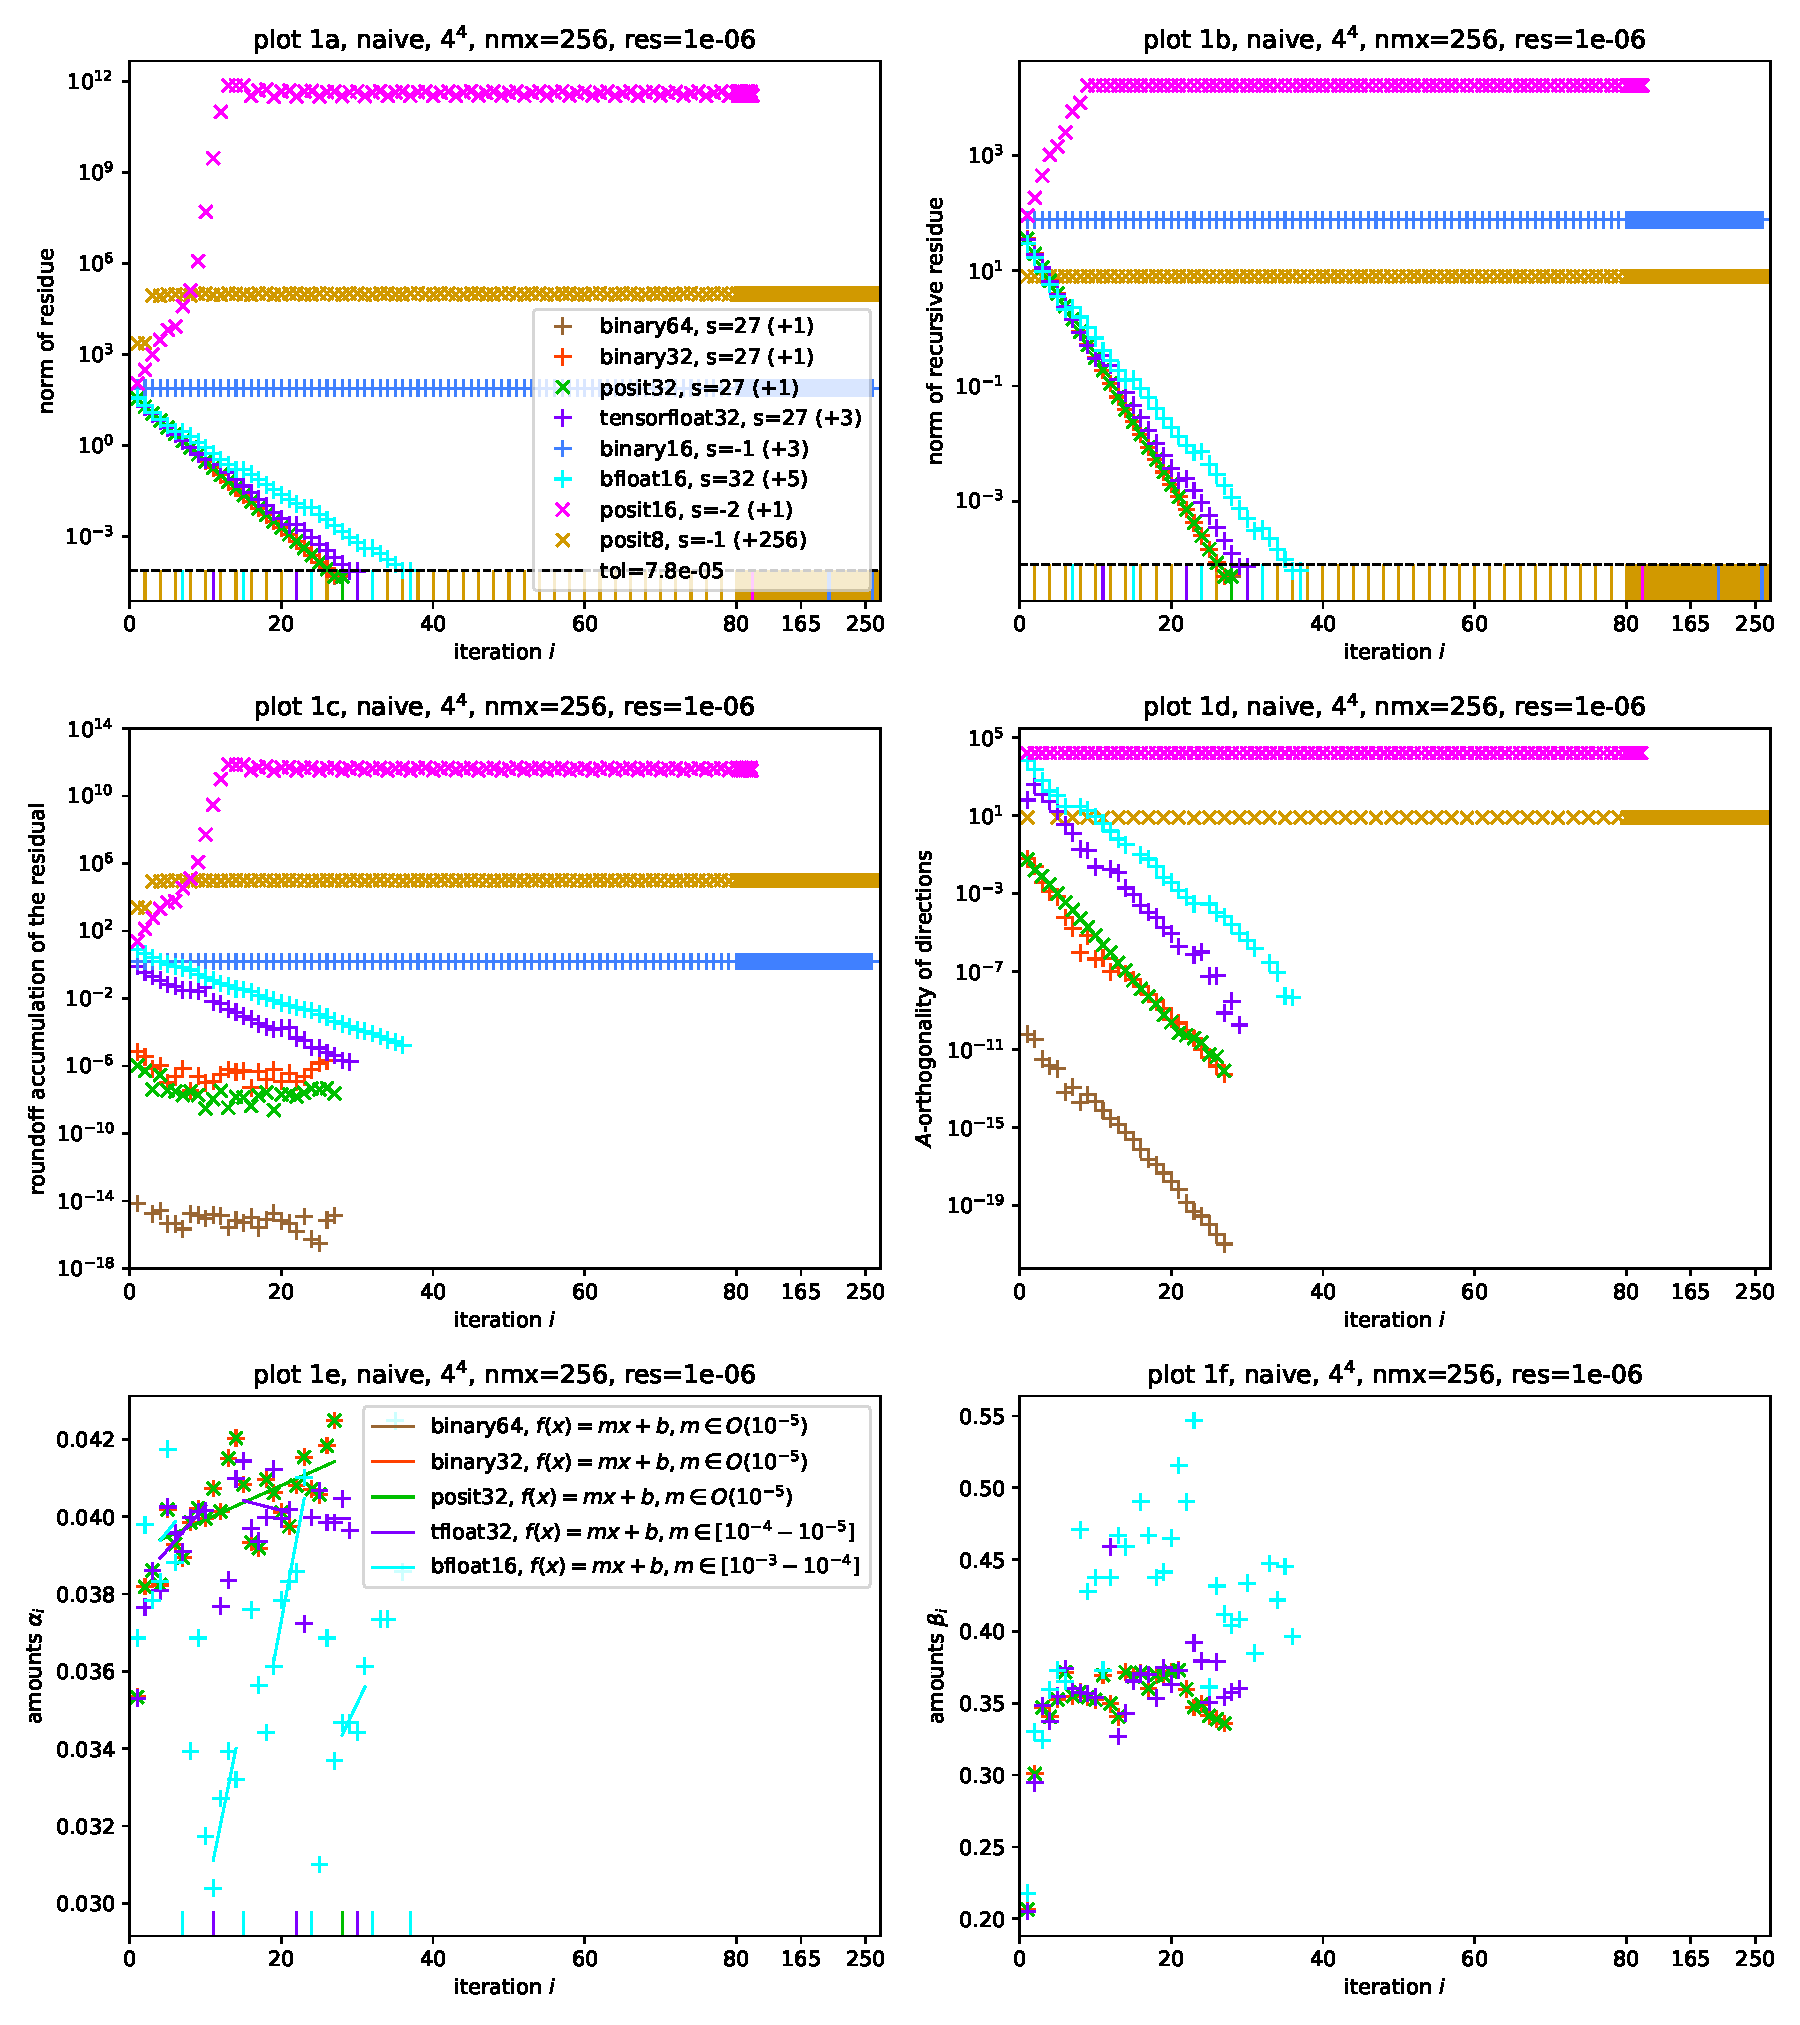
\includegraphics[width=1.0\linewidth]{plots/cgne_final_0}}
    %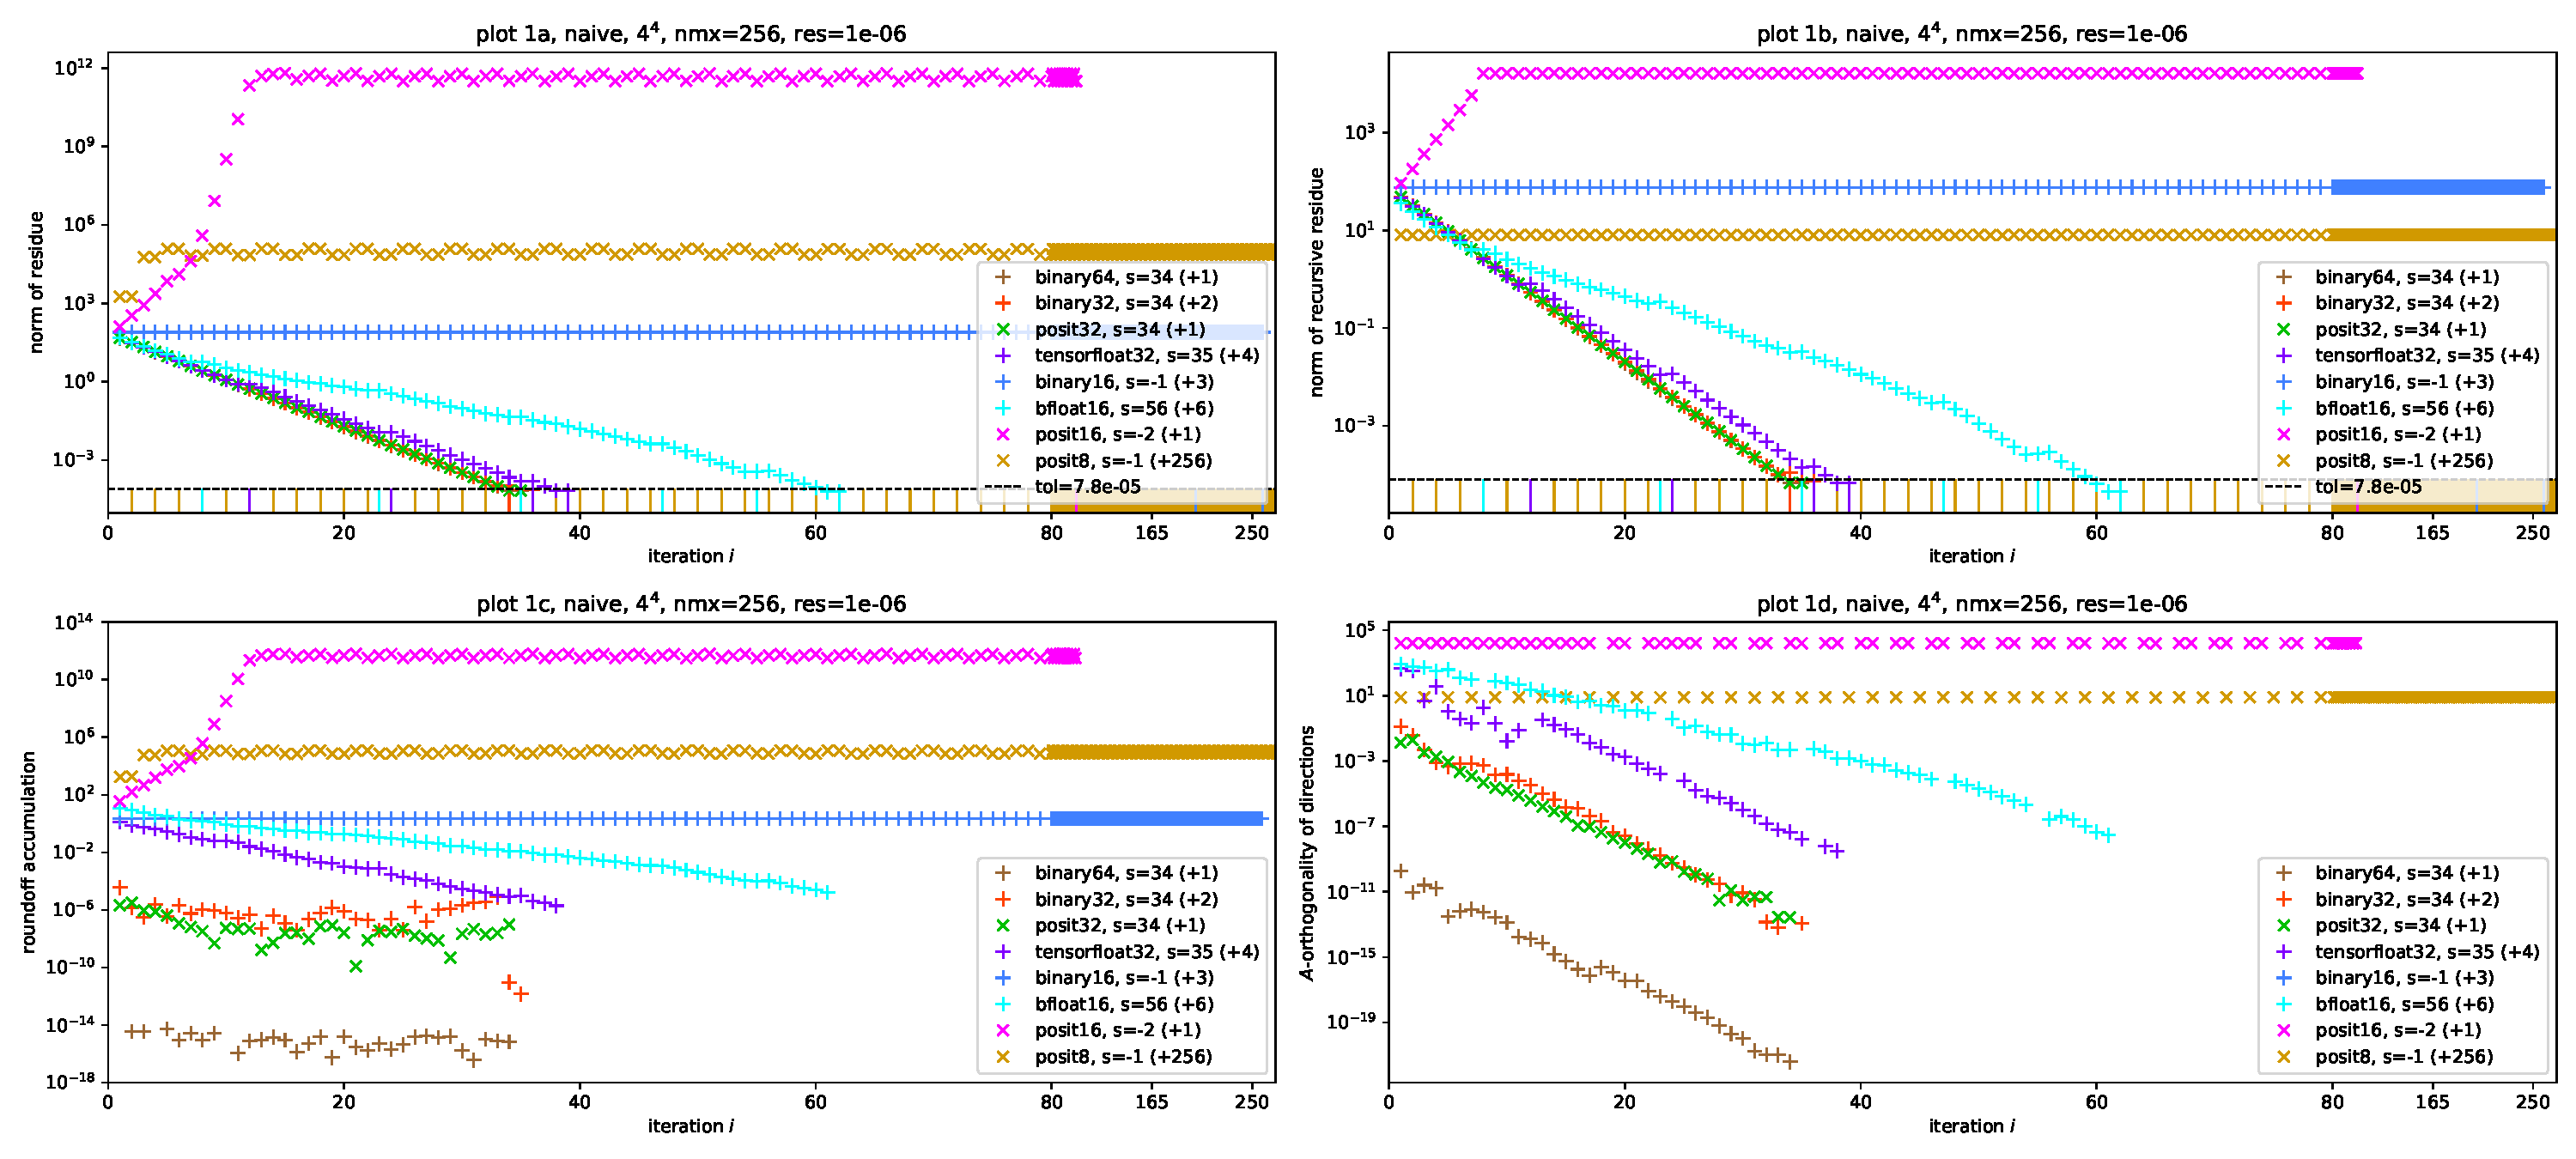
\includegraphics[width=1.0\textwidth]{plots/cgne0}
    \caption{Convergence analysis of a conjugate gradient run, where \gls{binary32} was replaced by one of the simulated data types. The number \code{s} describes the number of normal steps needed (the value of \code{status}), while the number in the brackets indicate the number of reset steps. The 6 plots show the naive replacement of the \gls{binary32} data type with the simulated one. This means that every single variable containing a \gls{binary32} was replaced with a variable of the simulated data type. Plot \textit{1a} shows the exact residue \eqref{eq:residual_exact} calculated in every iteration using the Dirac matrix and the source vector both in \gls{binary64}, while plot \textit{1b} shows the norm of the recursively calculated residue \eqref{eq:residual_recursive} (cast from the simulated data type to \gls{binary64}). The relative residue suffers from round-off accumulation because of the recursive calculation; this is the difference between plots \textit{1a} and \textit{1b}, which is plotted in plot \textit{1c}. Plot \textit{1d} shows the $A$-orthogonality of the current direction to the last direction, namely the value of $\vec{p}_{i-1}^\dagger A \vec{p}_{i}$. The last 2 plots, \textit{1e} and \textit{1f}, show the values of the amounts $\alpha_i$ and $\beta_i$ (see equations \eqref{eq:alphai} and \eqref{eq:betai}) in every iteration, but only of the data types that converged (\code{status>0}). The lines in plot \textit{1e} are linearly fitted to the data points ($f(x) = m x + b$). The number range of the slope $m$ is given in the plot legend.}
    \label{fig:cgne:naive}
\end{figure}

\begin{figure}
    \centering
    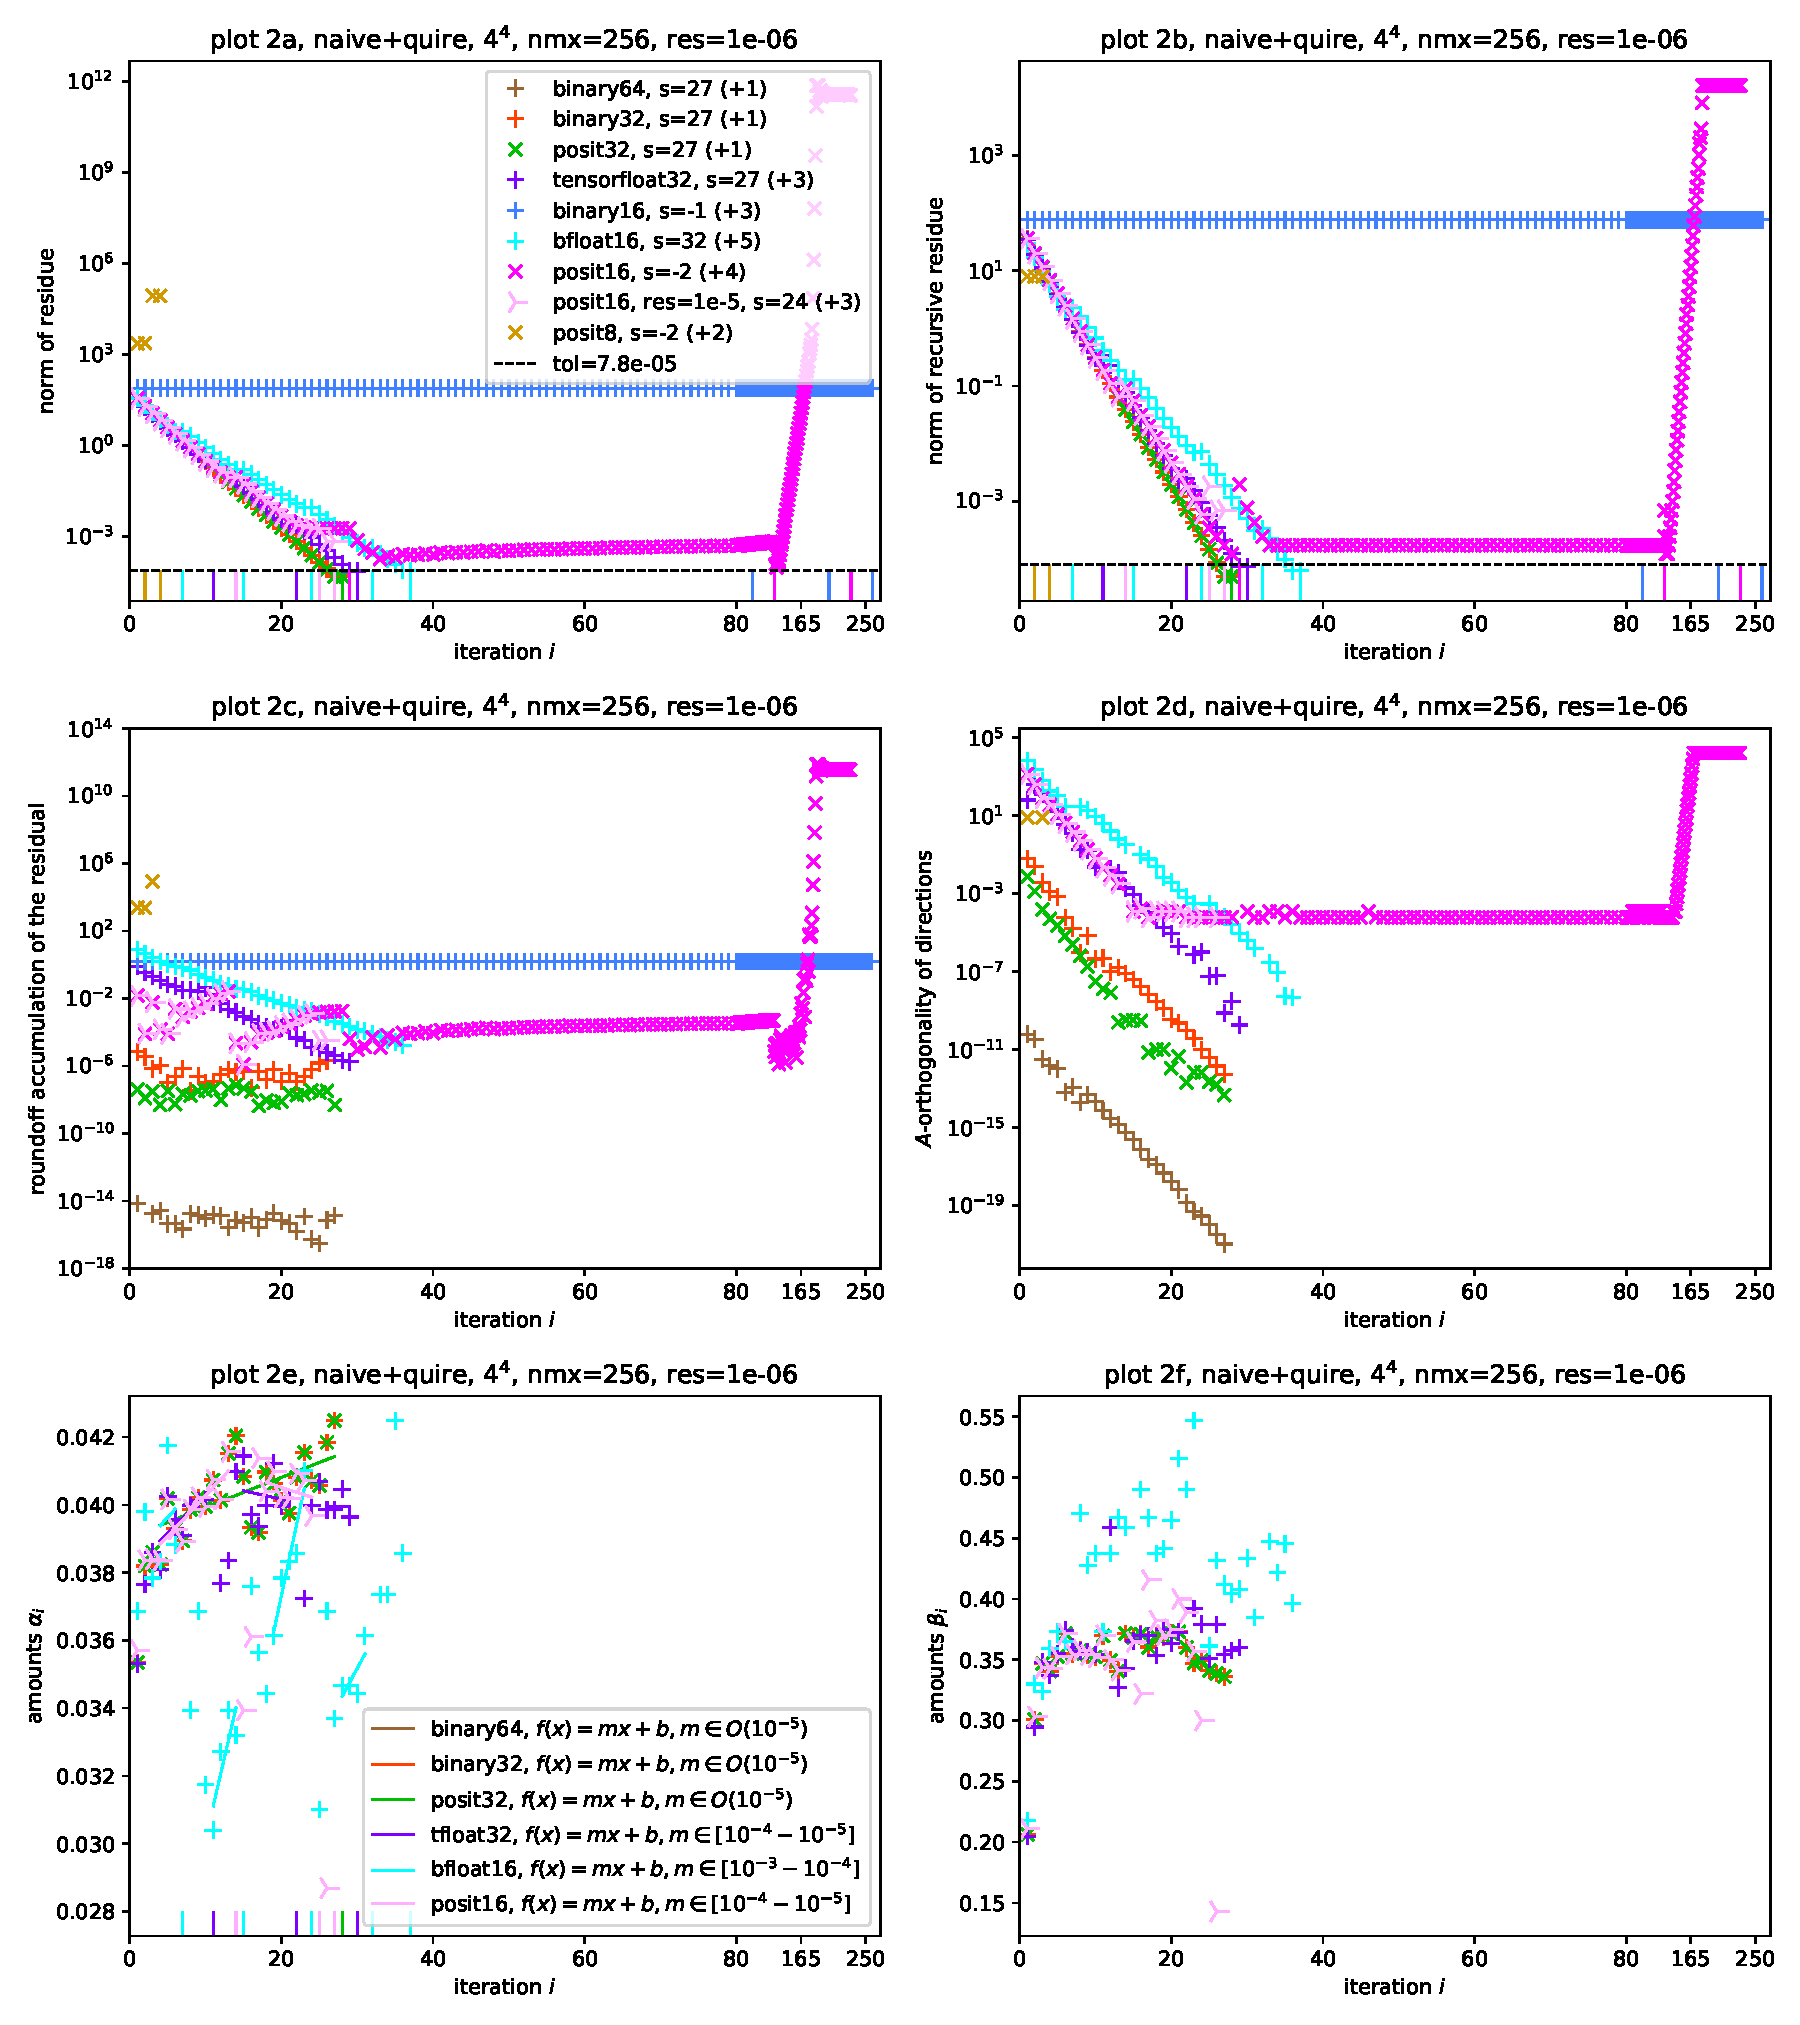
\includegraphics[width=1.0\textwidth]{plots/cgne_final_1}
    \caption{In these plots, the posits made use of \glspl{quire} as their collective variables, the remaining setup was the same as for figure \ref{fig:cgne:naive}, therefore the floating-point data types show exactly the same values, only posits changed their behaviour.}
    \label{fig:cgne:quire}
\end{figure}

\begin{figure}
    \centering
    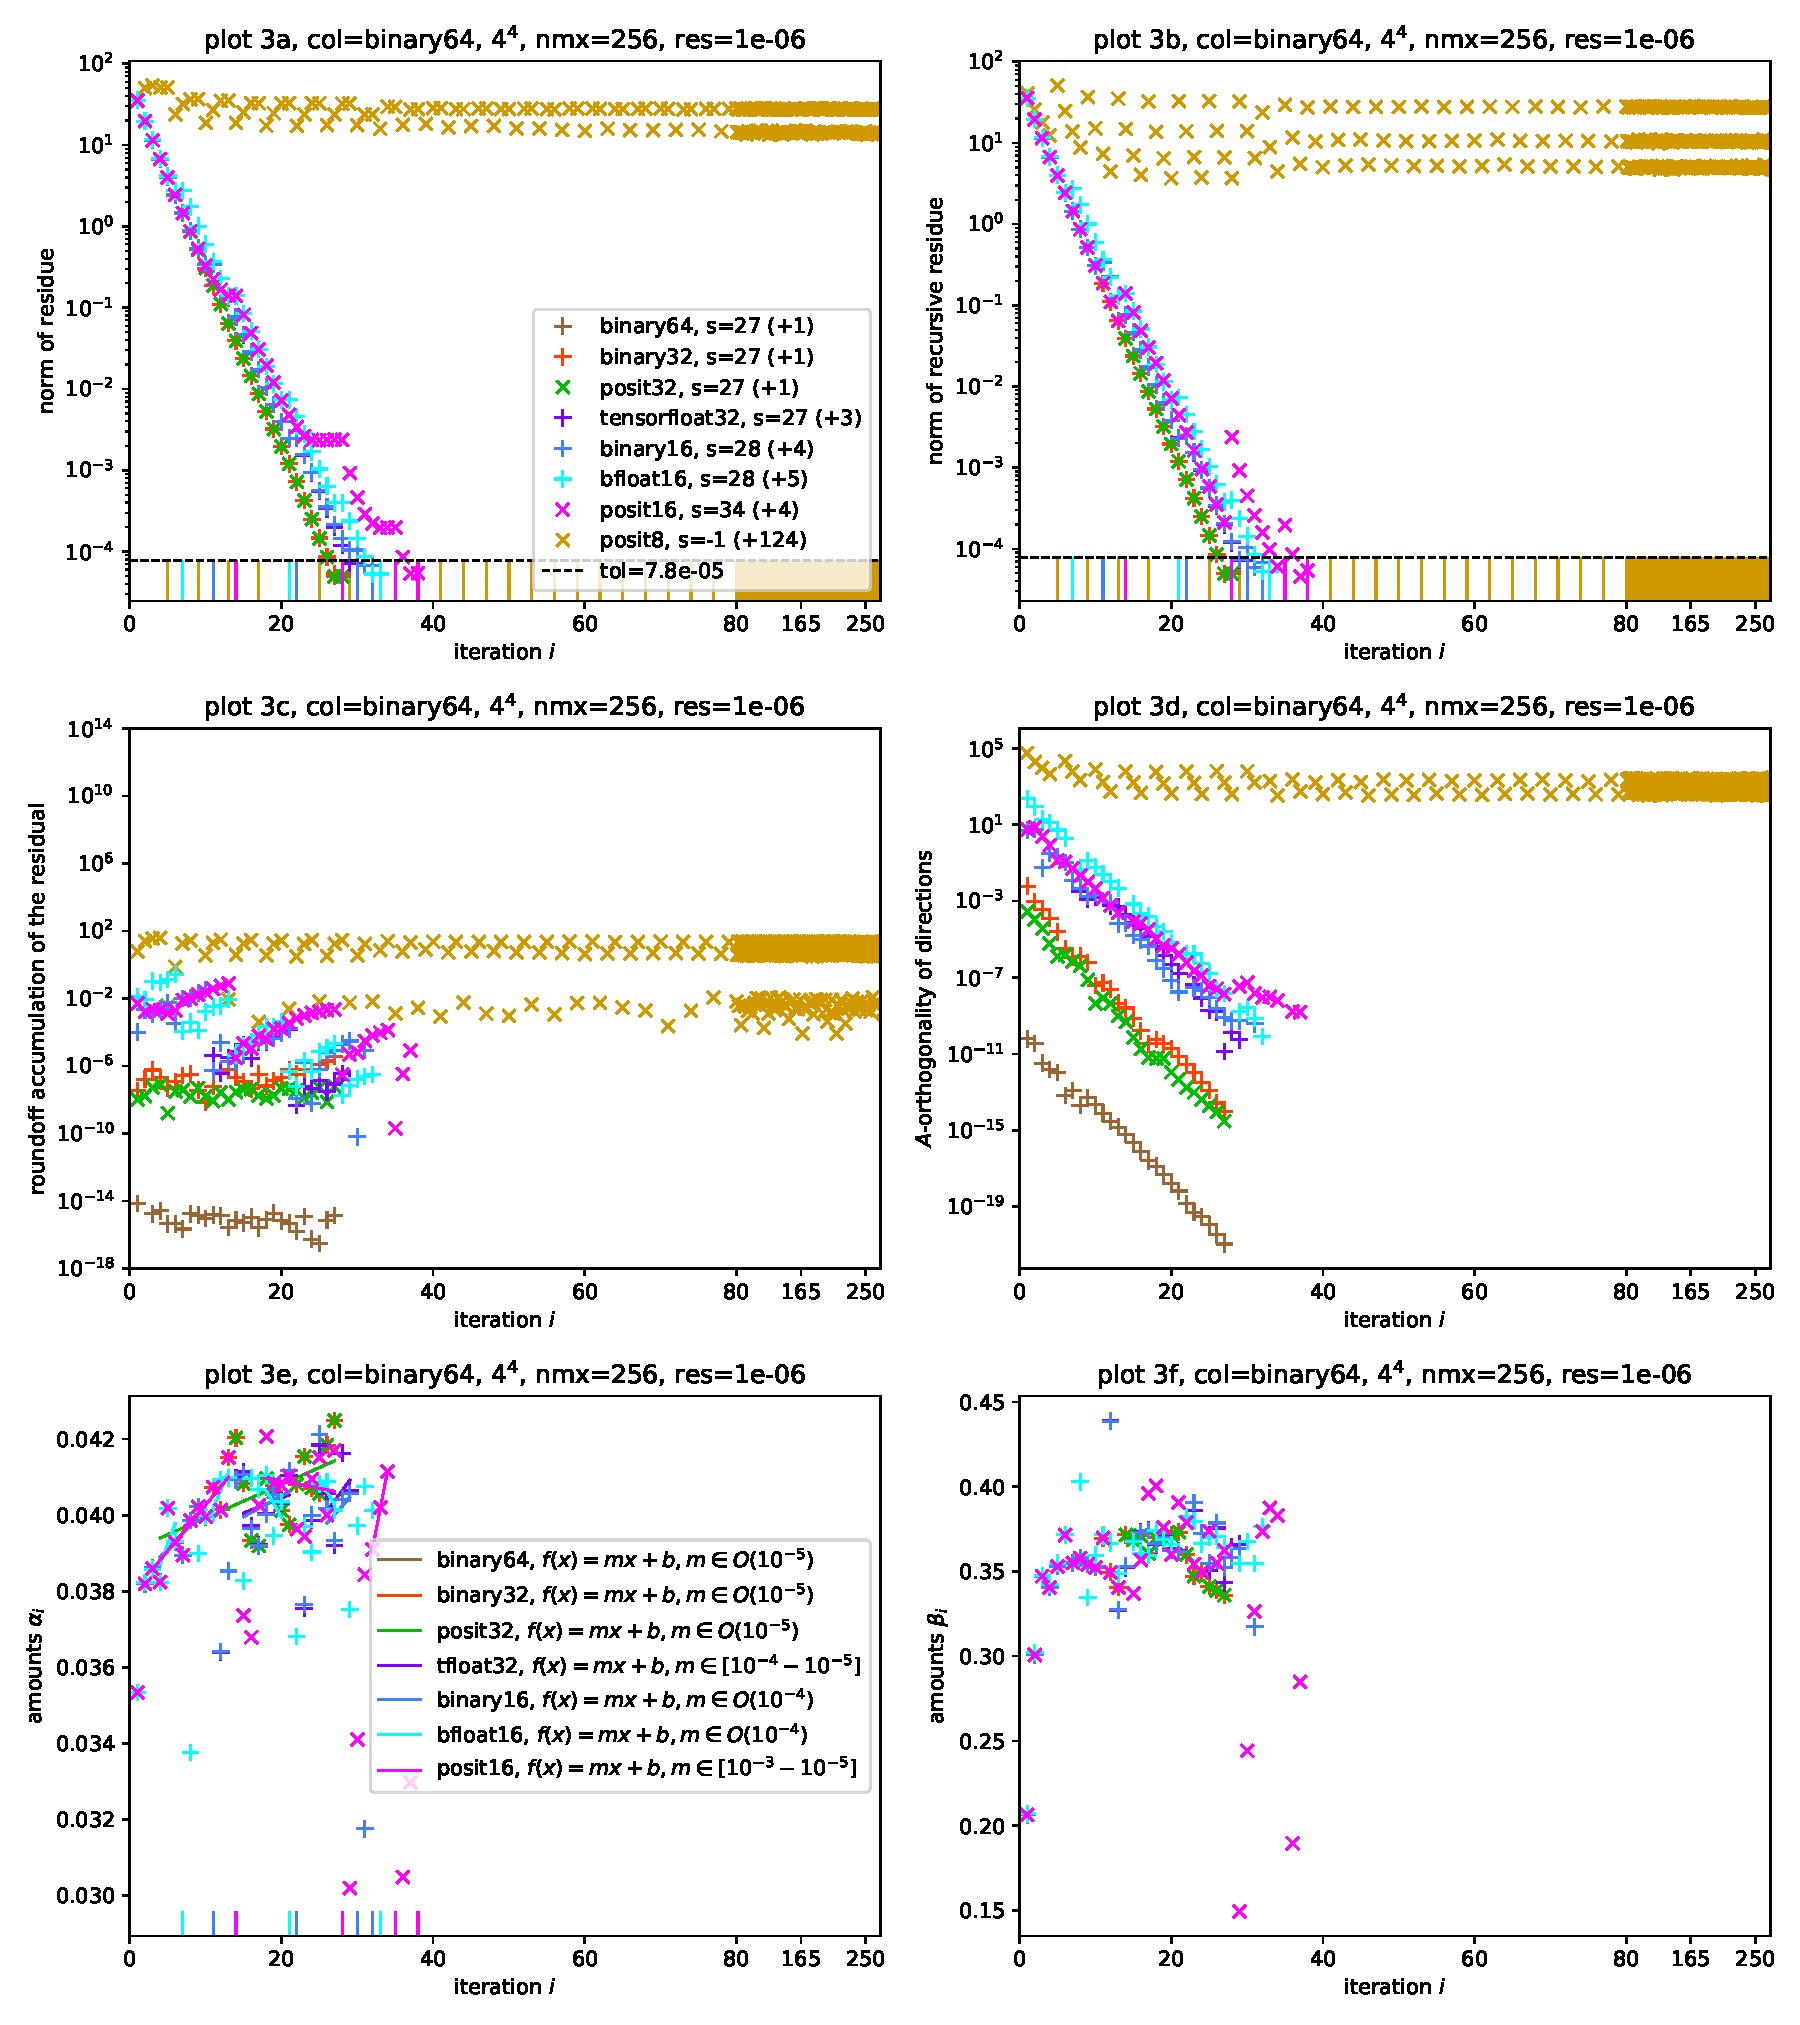
\includegraphics[width=1.0\textwidth]{plots/cgne_final_2}
    \caption{The 6 plots introduce a smarter replacement. All collective variables such as norms were calculated in \gls{binary64}, such that a data type with a small number range such as \gls{binary16} may not over- or underflow when calculating the norm of a vector full of said data type. This replacement resembles the \gls{quire} for posits. Using this replacement, even heavily reduced data types like \gls{binary16} and \gls{posit16} converged and threw a result of equal quality as the one simulated with \gls{binary64}.}
    \label{fig:cgne:col64}
\end{figure}


\begin{figure}
    \centering
    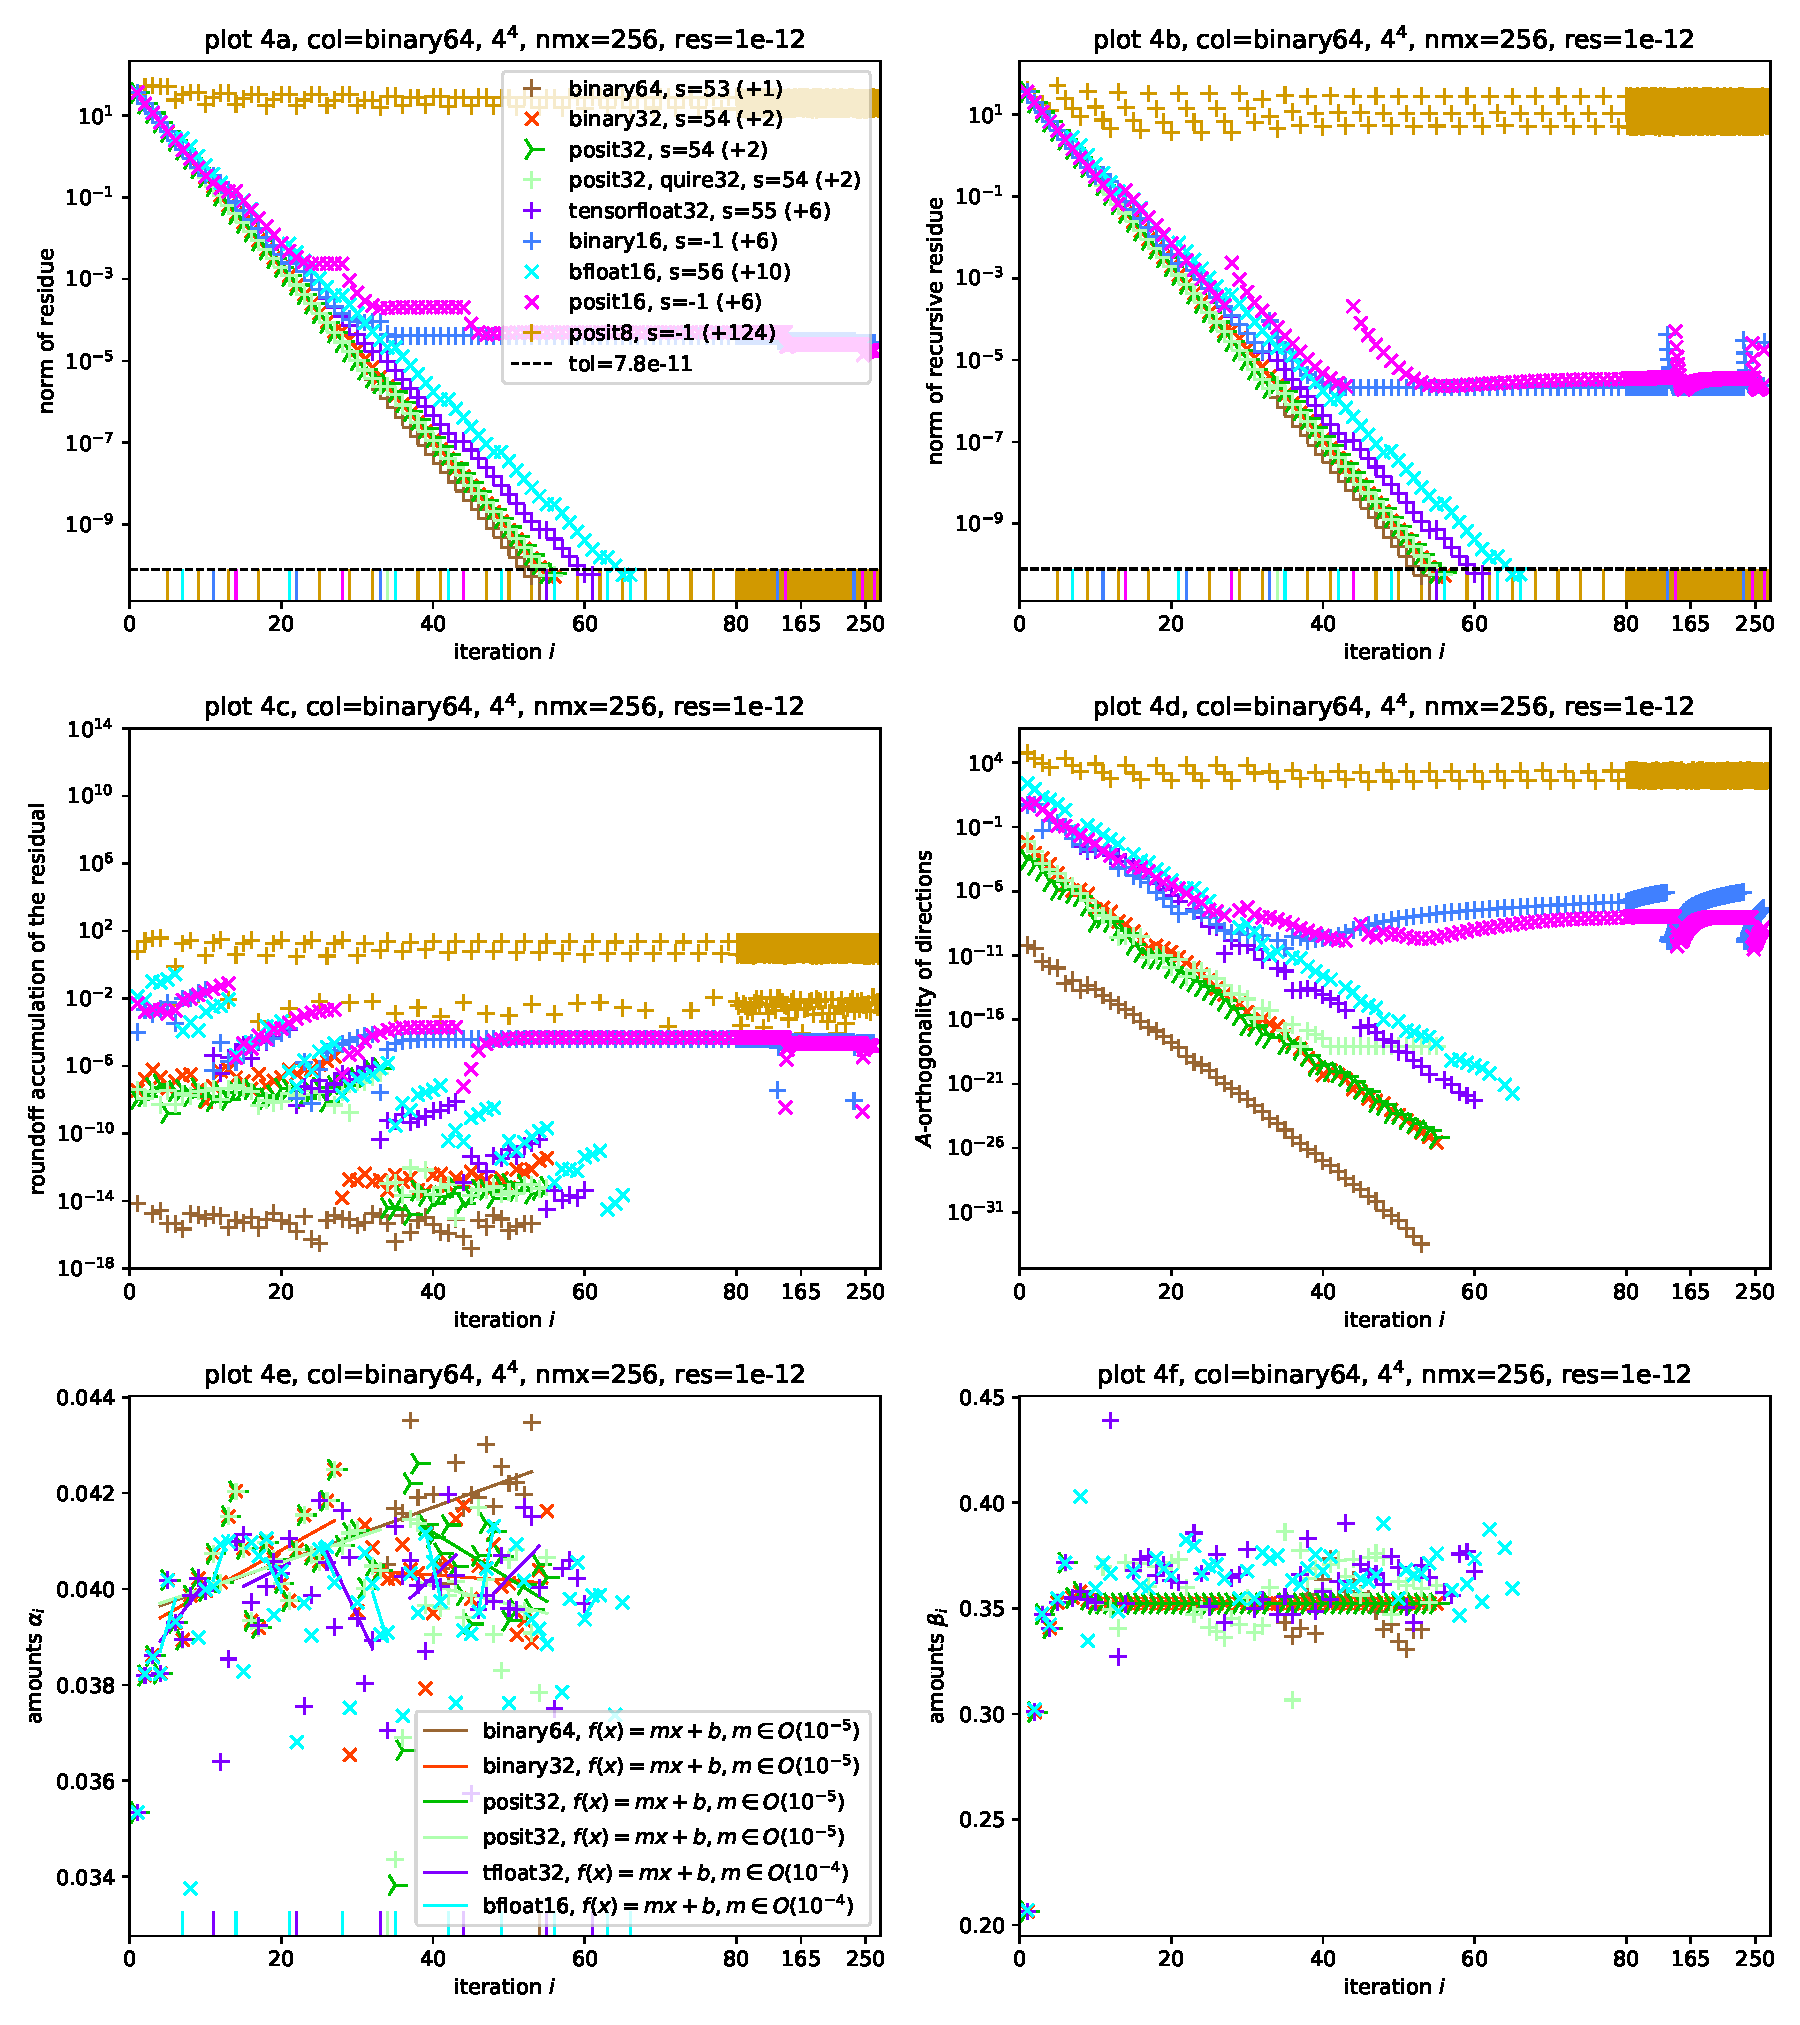
\includegraphics[width=1.0\textwidth]{plots/cgne_final_3}
    \caption{The configuration in this series of plots is equal to figure \ref{fig:cgne:col64}, besides the value of \code{res} -- the desired relative residue of the calculated solution -- is set to $10^{-12}$ instead of $10^{-6}$. Notice that $10^{-12}$ is outside the representable number range of the data types that did not converge; \gls{binary16}, \gls{posit16} and \gls{posit8}.}
    \label{fig:cgne:res12}
\end{figure}

\subsubsection{Discussion of figures \ref{fig:cgne:naive} - \ref{fig:cgne:res12}}

Figures \ref{fig:cgne:naive}, \ref{fig:cgne:quire}, \ref{fig:cgne:col64} and \ref{fig:cgne:res12} contain all relevant data. It is expected in general that the plots show data types of the same bit-length in clusters and exhibit a hierarchy in precision and exponent range; more precision and larger exponent range should end up in faster convergence. Thus, we expect the following hierarchy (where smaller means convergence in fewer steps)

\begin{align}
    \textcolor{cbrown}{\text{binary64}} < \textcolor{cgreen}{\text{posit32}} \leq \textcolor{cred}{\text{binary32}} \leq \textcolor{cpurple}{\text{tensorfloat32}} \leq \textcolor{cturquois}{\text{(1)}} \leq \textcolor{cpink}{\text{posit16}} \leq \textcolor{cblue}{\text{binary16}} \leq \textcolor{cturquois}{\text{(2)}} < \textcolor{cyellow}{\text{posit8}}, \label{eq:hierarchy}
\end{align}

where \textcolor{cturquois}{\text{bfloat16}} could be either at position \textcolor{cturquois}{\text{(1)}} or \textcolor{cturquois}{\text{(2)}}, depending on what is more important, precision or number range.

\textbf{Figure \ref{fig:cgne:naive}:} In figure \ref{fig:cgne:naive} where the original data type is naively\footnote{Naive in this context means that \textit{all} appearances of binary32-variables in the cgne-kernel were blindly replaced by variables of simulated data type.} replaced by the simulated data type, it can be concluded that only data types with large enough number ranges converged. \gls{binary64}, \gls{binary32} and \gls{posit32} converged each after \code{status=27} steps with one reset step. The less precise \gls{tensorfloat32} took \code{status=27} ($+3$) and the even less precise \gls{bfloat16} required \code{status=32} ($+5$) steps. Such a hierarchical result was expected since they have the same exponent range and thus approximately the same number range but differ only in precision (see table \ref{tab:formats}). Notice that the less precise the data type, the more reset steps are needed. This happens because the precision limit of the simulated data type is reached earlier if the data type has less precision.

The round-off accumulation error of \gls{posit32} is slightly better than the one of \gls{binary32}, although defeated by $8$ orders of magnitude of \gls{binary64} because of its much more precision. It is notable to remark that the round-off accumulation does not increase significantly in successice steps, what would be expected from a recursive calculation. The reason for the small difference between \gls{binary32} and \gls{posit32} could be that the involved real numbers are closer to representable numbers in \gls{posit32} than in \gls{binary32}. Posits have a larger number density around \num{1} compared to floats of the same bit-length, and therefore more precision in that regime (see figure \ref{fig:number_line} for the example of \gls{binary16} vs. \gls{posit16}). Posits also have more numbers because they have no \acrshortpl{nan}. Round-off accumulation depends crucially on the precision of the data type; the lower the precision, the higher the round-off accumulation. The difference in $A$-orthogonality is negligible for \gls{posit32} compared to \gls{binary32}, but clearly surpassed by \gls{binary64}.

\gls{binary16} did not converge (\code{status=-1}) after the maximal number of \code{nmx=256} steps. Its footprint is absent in plot \textit{1d}, because it consisted only of \acrshortpl{nan} and infinities, causing $\alpha_i = 0$ and $\beta_i = 1$. This implied that $\vec{r}_i = \vec{r}_{i+1}$ and $\vec{p}_{i+1} = \vec{r}_{i+1}$ and therefore $\vec{x}_{i+1} = \vec{x}_{i}$ and the algorithm stalled. This explains why the residues don't change in plots \textit{1a} and \textit{1b}. The reason for the first infinity was an overflow when calculating the norm of $\vec{b}$ in the very first iteration. This suggests that the limited number range of \gls{binary16} might not be enough (at least for a naive replacement), comparing to \gls{bfloat16} with the same bit-length, but larger number range that was able to converge, although very slowly.

The behaviour of \gls{posit8} is similar to \gls{binary16}, but without the overflow, because posits do not overflow by definition. Instead, the largest representable number is returned or in case of an underflow the smallest representable number is returned \cite{posit2018standard}. The algorithm stalled at a value $\norm{\vec{r}_i} = 8$ of the recursive residual norm. The largest \num{8}-bit posit number with exponent bits $es=0$ is $2^6 = 64$, thus the norm squared cannot be greater than $64$ and the norm itself cannot be larger than $8 = \sqrt{64}$ (see plot \textit{1b}). This happened in the first step, where the actual residual in \gls{binary64} was $\backsim 10^3$. The amounts $|\alpha_i| \ll 1$ in iterative steps are therefore negligibly small causing $\vec{x}_{i+1} \approx \vec{x}_i$. Significant changes in $\vec{x}_i$ will not happen and convergence is unlikely. Notice that \gls{posit8} had \num{256} reset steps, which means that after every step there was a reset step. The steps were caused by the low precision (and thus high machine epsilon) of \gls{posit8}. The value of \code{PRECISION\_LIMIT} is $100*\code{MACHINE\_EPSILON}$, which takes a value of \num{3.125} for \gls{posit8}.

Similarly, for \gls{posit16}, the maximal representable value with $es=1$ is \num{268435456} whose square root is \num{16384} which is reached after $8$ steps (see plot \textit{1b}). The actual residual in the $8$-th step was $\backsim 10^7$, the algorithm diverged and then stalled. Iterative steps are therefore mostly too small, and convergence is unlikely.

We observe that number range is more important than precision, when naively replacing the data type, but the higher the precision, the faster the convergence and the fewer reset steps are needed.

\textbf{Figure \ref{fig:cgne:quire}:} In figure \ref{fig:cgne:quire} posits made use of the \gls{quire}. Therefore, the numbers for the float data types are exactly equal to the ones in figure \ref{fig:cgne:naive}, because floats have no such feature. They are not further discussed.

Comparing plots \textit{1c} and \textit{2c} and looking at \gls{posit32}, one can see that the round-off accumulation in the residual due to its recursive calculation is slightly better than without using the \gls{quire}. This makes sense, because \glspl{quire} introduce deferred rounding. The entire run thus involved less rounding. This is exploited in the calculation of norms and matrix-vector products. It results in a somewhat better maintaining of $A$-orthogonality for the direction vectors.

However, the data points of \gls{posit16} bear little resemblance to their previous or later runs. They come much closer to the target residual tolerance than in the last simulation, but the tolerance is still not reached. The tolerance is within the number range of \gls{posit16}, even so it did not converge. The reason for this is that the smallest representable number in \gls{posit16} is $2^{-28}$. The \gls{quire} for \gls{posit16} has the same number range, despite the \num{128} bits in length. Every norm squared of a non-zero vector must be larger or equal to this number, because posit do not underflow. Therefore, the norm is always greater or equal to $\sqrt{2^{-28}} = 2^{-14} \approx 6.1 \cdot 10^{-5}$. The tolerance of $7.8 \cdot 10^{-5}$ -- even though larger than that number -- is perhaps still too close. Comparing the \textcolor{clightpink}{lightpink} values, that are \gls{posit16} as well, but the relative residual \code{res} is set to $10^{-5}$ instead (the tolerance being one order of magnitude larger), they converged after only \code{status=24} steps. This suggests that the reason for the strange behaviour lies in the relative residual that was chosen too close to the lowest number above zero of the number regime.

Using the same arguments and analysis, \gls{posit8} did not give a meaningful result.

\textbf{Figure \ref{fig:cgne:col64}:} In figure \ref{fig:cgne:col64}, a smarter replacement was done. All reduction variables that have a collective role suffer from overflow. For example, the norm of a vector $\vec{v} \in \mathbb{R}^n$ is 

\begin{align*}
    \norm{\vec{v}} = \sqrt{ \sum_{i=1}^{n} v_i^2 }.
\end{align*}

The number below the square root may be much bigger before squaring than after. If we calculate the norm in \gls{posit8}, the result will be $\norm{\vec{y}} \leq 8$. More importantly, when using a data type that overflows such as \gls{binary16}, the value after squaring might be perfectly fine, but the value under the square root could be outside the range of representable numbers, $\sqrt{\infty} = \infty$ and $\sqrt{0} = 0$. This is avoided if the collective variable is of a data type with larger number range than the underlying data type that is summed over. In figure \ref{fig:cgne:col64} all reduction variables were of type \gls{binary64}.

The data of \gls{binary64} exhibits no significant alterations. Again comparing \gls{binary32} and \gls{posit32} with their previous data points, we see that the round-off accumulation of \gls{binary32} is a little better, while \gls{posit32} looks the same as with the \gls{quire}, suggesting that when using posits employing the \gls{quire} is probably sufficient.

Looking at \gls{tensorfloat32}, it has the same exponent range as \gls{binary32}, but less precision and it has the same number of mantissa bits as \gls{binary16}, but at a higher exponent range. Compared to \gls{binary16}, both data types have the same amount of numbers to be distributed in their respective number range. It is expected to perform worse or equal to \gls{binary32}, but better or equal to \gls{binary16} and \gls{bfloat16}. Therefore, it's expected to converge in $27 \le \code{status} \le 28$ steps, see equation \eqref{eq:hierarchy}. This is indeed the case with \code{status=27} steps. We see that the larger number range compared to \gls{binary16} has little effect on the speed of convergence. This is because the number regime is within the \gls{binary16} regime, except for reduction variables. This explains as well why \gls{tensorfloat32} performed precisely as in the naive replacement, figure \ref{fig:cgne:naive}, but the round-off accumulation is better because of the more precise reduction variables.

The \gls{bfloat16} with even less precision but comparable number range of \gls{tensorfloat32} converged in \code{status=28} steps as well, but required two more reset steps, tightening the previous conclusion about speed of convergence.

The most interesting data points are the ones of \gls{binary16} and \gls{posit16} that both were able to converge in \code{status=28} and \code{status=34} steps, respectively. They performed quite similar, even though it would be expected that \gls{posit16} would perform slightly better because of the increased number range and larger number density in the relevant number regimes (see figure \ref{fig:number_line}). In plot \textit{3c} the increase of round-off accumulation can be observed for \gls{binary16} and \gls{posit16} in steps where the real residue changes (where the algorithm makes progress, see for example: steps \num{1} to \num{10}). Notice that, when the real residue stalls and the recursive residue still (wrongly) decreases, the round-off accumulation will saturate until the orders of magnitude of the two numbers differs too much such that their difference is dominated by the larger number. This can be seen in the data points of \gls{posit16} in plot \textit{3a}. It suggests that the precision limit was chosen too low for the data type. Notice that the precision limit is defined to be \code{100*MACHINE\_EPSILON}, where \code{MACHINE\_EPSILON} depends on the data type. The \code{MACHINE\_EPSILON} for the posit data types is quite misleading, because it gives us (by definition) the precision of numbers around \num{1}. This is the regime where posits are most precise, their precision falling off very rapidly when leaving it. Thus for \gls{posit16} in the regime $10^{-1}$ the \code{MACHINE\_EPSILON} is correct (seen at iteration \num{14}), while in the regime $10^{-3}$ it is chosen to small and we can see a staircase-shape around the reset steps at iterations \num{28} and \num{35}. Such a stalling of the real residue should be avoided at any cost because the algorithm stalls as well in that case. The \code{MACHINE\_EPSILON} is defined to be the difference between \num{1} and the lowest number above \num{1}. For floats this definition makes more sense, because their precision does not fall off that rapidly, but for posits which are most precise around \num{1}, this gives a too precise value, not reflecting the real precision of posits in their entire number range correctly. Instead, the machine epsilon should be a function of the number regime, increasing when going far away from \num{1}. This is the reason for the staircase-shaped curve of \gls{posit16} in plot \textit{3a}. This phenomenon is even more prominent for \gls{posit16} in plot \textit{4a} of figure \ref{fig:cgne:res12}. \Gls{posit32} does not have this problem, because its \code{MACHINE\_EPSILON} is sufficient for the number regime used in the algorithm. When demanding lower relative residuals, staircase-shapes should be expected for \gls{posit32} as well.

Comparing \gls{binary16} with \gls{bfloat16} and \gls{tensorfloat32}, we see again that exponent range is less relevant than precision, but precision determines the amount of reset steps.

\textbf{Figure \ref{fig:cgne:res12}:} Figure \ref{fig:cgne:res12} shows all the simulated data types using a reduction data type of \gls{binary64} as in figure \ref{fig:cgne:col64}, but with a relative residual of $10^{-12}$ instead. The last row resembles the predicted hierarchy \eqref{eq:hierarchy} particularly well. Notice that $10^{-12}$ is outside the representable number range of \gls{binary16}, \gls{posit16} and \gls{posit8}. This means that these data types cannot reach the target tolerance, therefore we didn't expect them to converge. This is indeed the case. Furthermore, we see that \gls{binary16} and \gls{posit16} both are not able to go below $10^{-5}$, meaning the tolerance in the third row was chosen close to the minimum, but still converging tolerance (see discussion of \gls{posit16} in figure \ref{fig:cgne:quire}). Both data types make no further considerable progress after step \num{45}. It can be seen by the recursive residue stalling or even increasing -- an indicator that the data type has reached its limits.

The comparison between \gls{binary32} and \gls{posit32} is again of insight. Their difference is subtle. We see that both required the same number of steps. Round-off accumulation and $A$-orthogonality are again slightly better, making \gls{posit32} the overall better \num{32}-bit data type for the problem. The reason for this is due to the higher precision of posits in the relevant number regime. Looking at the \textcolor{clightgreen}{lightgreen} values, that are \gls{posit32} as well, but utilising the \gls{quire} instead of \gls{binary64} as collective reduction variable, we observe the same number of steps to convergence, but round-off accumulation is slightly worse. It might be an unfair comparison, because \gls{binary64} as collective variable has more precision, surpassing even the deferred rounding employed by the \num{512}-bit \gls{quire} for \gls{posit32}. In plot \textit{4d} the \gls{posit32} with \gls{quire} will not go below some fixed value. The reason for this is the lowest \gls{posit32} value with exponent bits \code{es=2} is $8^{-30}$ and the norm of a \gls{posit32}-vector with at least one non-zero component must be greater or equal to the square root, $1.15 \cdot 10^{-18}$. This suggests that when choosing \code{res} to be smaller than $10^{-18}$, we expect \gls{posit32} to not converge anymore in analogy to \gls{posit16} in the second row.

Since \gls{binary16} was able to converge in figure \ref{fig:cgne:col64}, suggesting that the number regime is within \gls{binary16}, which gives \gls{posit32} more precision in that regime over \gls{binary32}

Finally, we compare the three data types with the same exponent range, but different precisions; \gls{binary32}, \gls{tensorfloat32} and \gls{bfloat16}. The less precision, the slower the convergence. The price to go from \num{23} to \num{10} mantissa bits results in \num{1} more conjugate gradient step as well as \num{4} more reset steps. When going further down to \num{7} mantissa bits again \num{1} more regular step and \num{4} more reset steps where needed to finally bring \gls{bfloat16} to convergence after \code{status=56} regular conjugate gradient plus \num{10} reset steps. Bearing in mind that it uses only \num{16} bits, this is a remarkable result. It performed way better than its \num{16}-bit competitors.

As seen in plot \textit{4a}, all data types start to converge by the same speed (all slopes are equal). The actual residual of the data type with the lowest precision, namely \gls{bfloat16} with \num{7} mantissa bits, resets first, followed by \gls{binary16} and \gls{tensorfloat32} which have both \num{10} mantissa bits. The next one is \gls{posit16}, because it has more precision than \gls{binary16} in the relevant regime, followed by \gls{binary32} with \num{23} mantissa bits and later by \gls{posit32}, where the same argument as before holds. The curve of \gls{binary64} would also reset at some point, but that is outside the scale.

Specially plot \textit{4a} suggests that we can start to calculate in a data type with \num{16} bits of length until we fall below a constant value (to be determined and depending on the data type), then continuing the calculation in a data type with \num{32} bit-length until that number regime is exhausted as well, again switching to a \num{64} bit data type to finish the calculation.

\subsubsection{$8^4$ lattice}

To make sure that the previous analysis is consistent, and the physics involved were relevant, the same data was extracted from an $8^4$ lattice and some of the plots were remade from the new data, see figure \ref{fig:cgne8}. Only the data types \gls{binary64}, \gls{binary32} and \gls{binary16} were simulated. The main difference to figures \ref{fig:cgne:col64} and \ref{fig:cgne:res12} is that more steps were required to converge, because the Dirac matrix is much larger than before, although only \num{0.04}\% of all components were non-zero, compared to \num{2}\% in the $4^4$ lattice of the previous analysis. In plots \textit{2a} to \textit{2f}, where the relative residue was chosen to be $10^{-12}$, we again see the saturation of \gls{binary16} marking the lower limit of the data type. After every reset step, a jump in round-off accumulation can be seen, because the residual in the reset step is calculated in higher precision. It is interesting that the round-off accumulation in the final steps of \gls{binary16} come remarkably close to those of \gls{binary32} (see plot \textit{1c}). A reason for this could be the clustering of reset steps just before convergence, giving accurate results with little round-off, even for less precise data types. Furthermore, we see the speed of convergence does not significantly depend on the precision of the data type, only the amount of reset steps does, thus the less steep slope of \gls{binary16}. When the lower limit of the data type is reached, the slope becomes zero and the residual shows no striking change anymore. This is where the data type should be switched to one with a larger number range.

\begin{figure}[h]
    \centering
    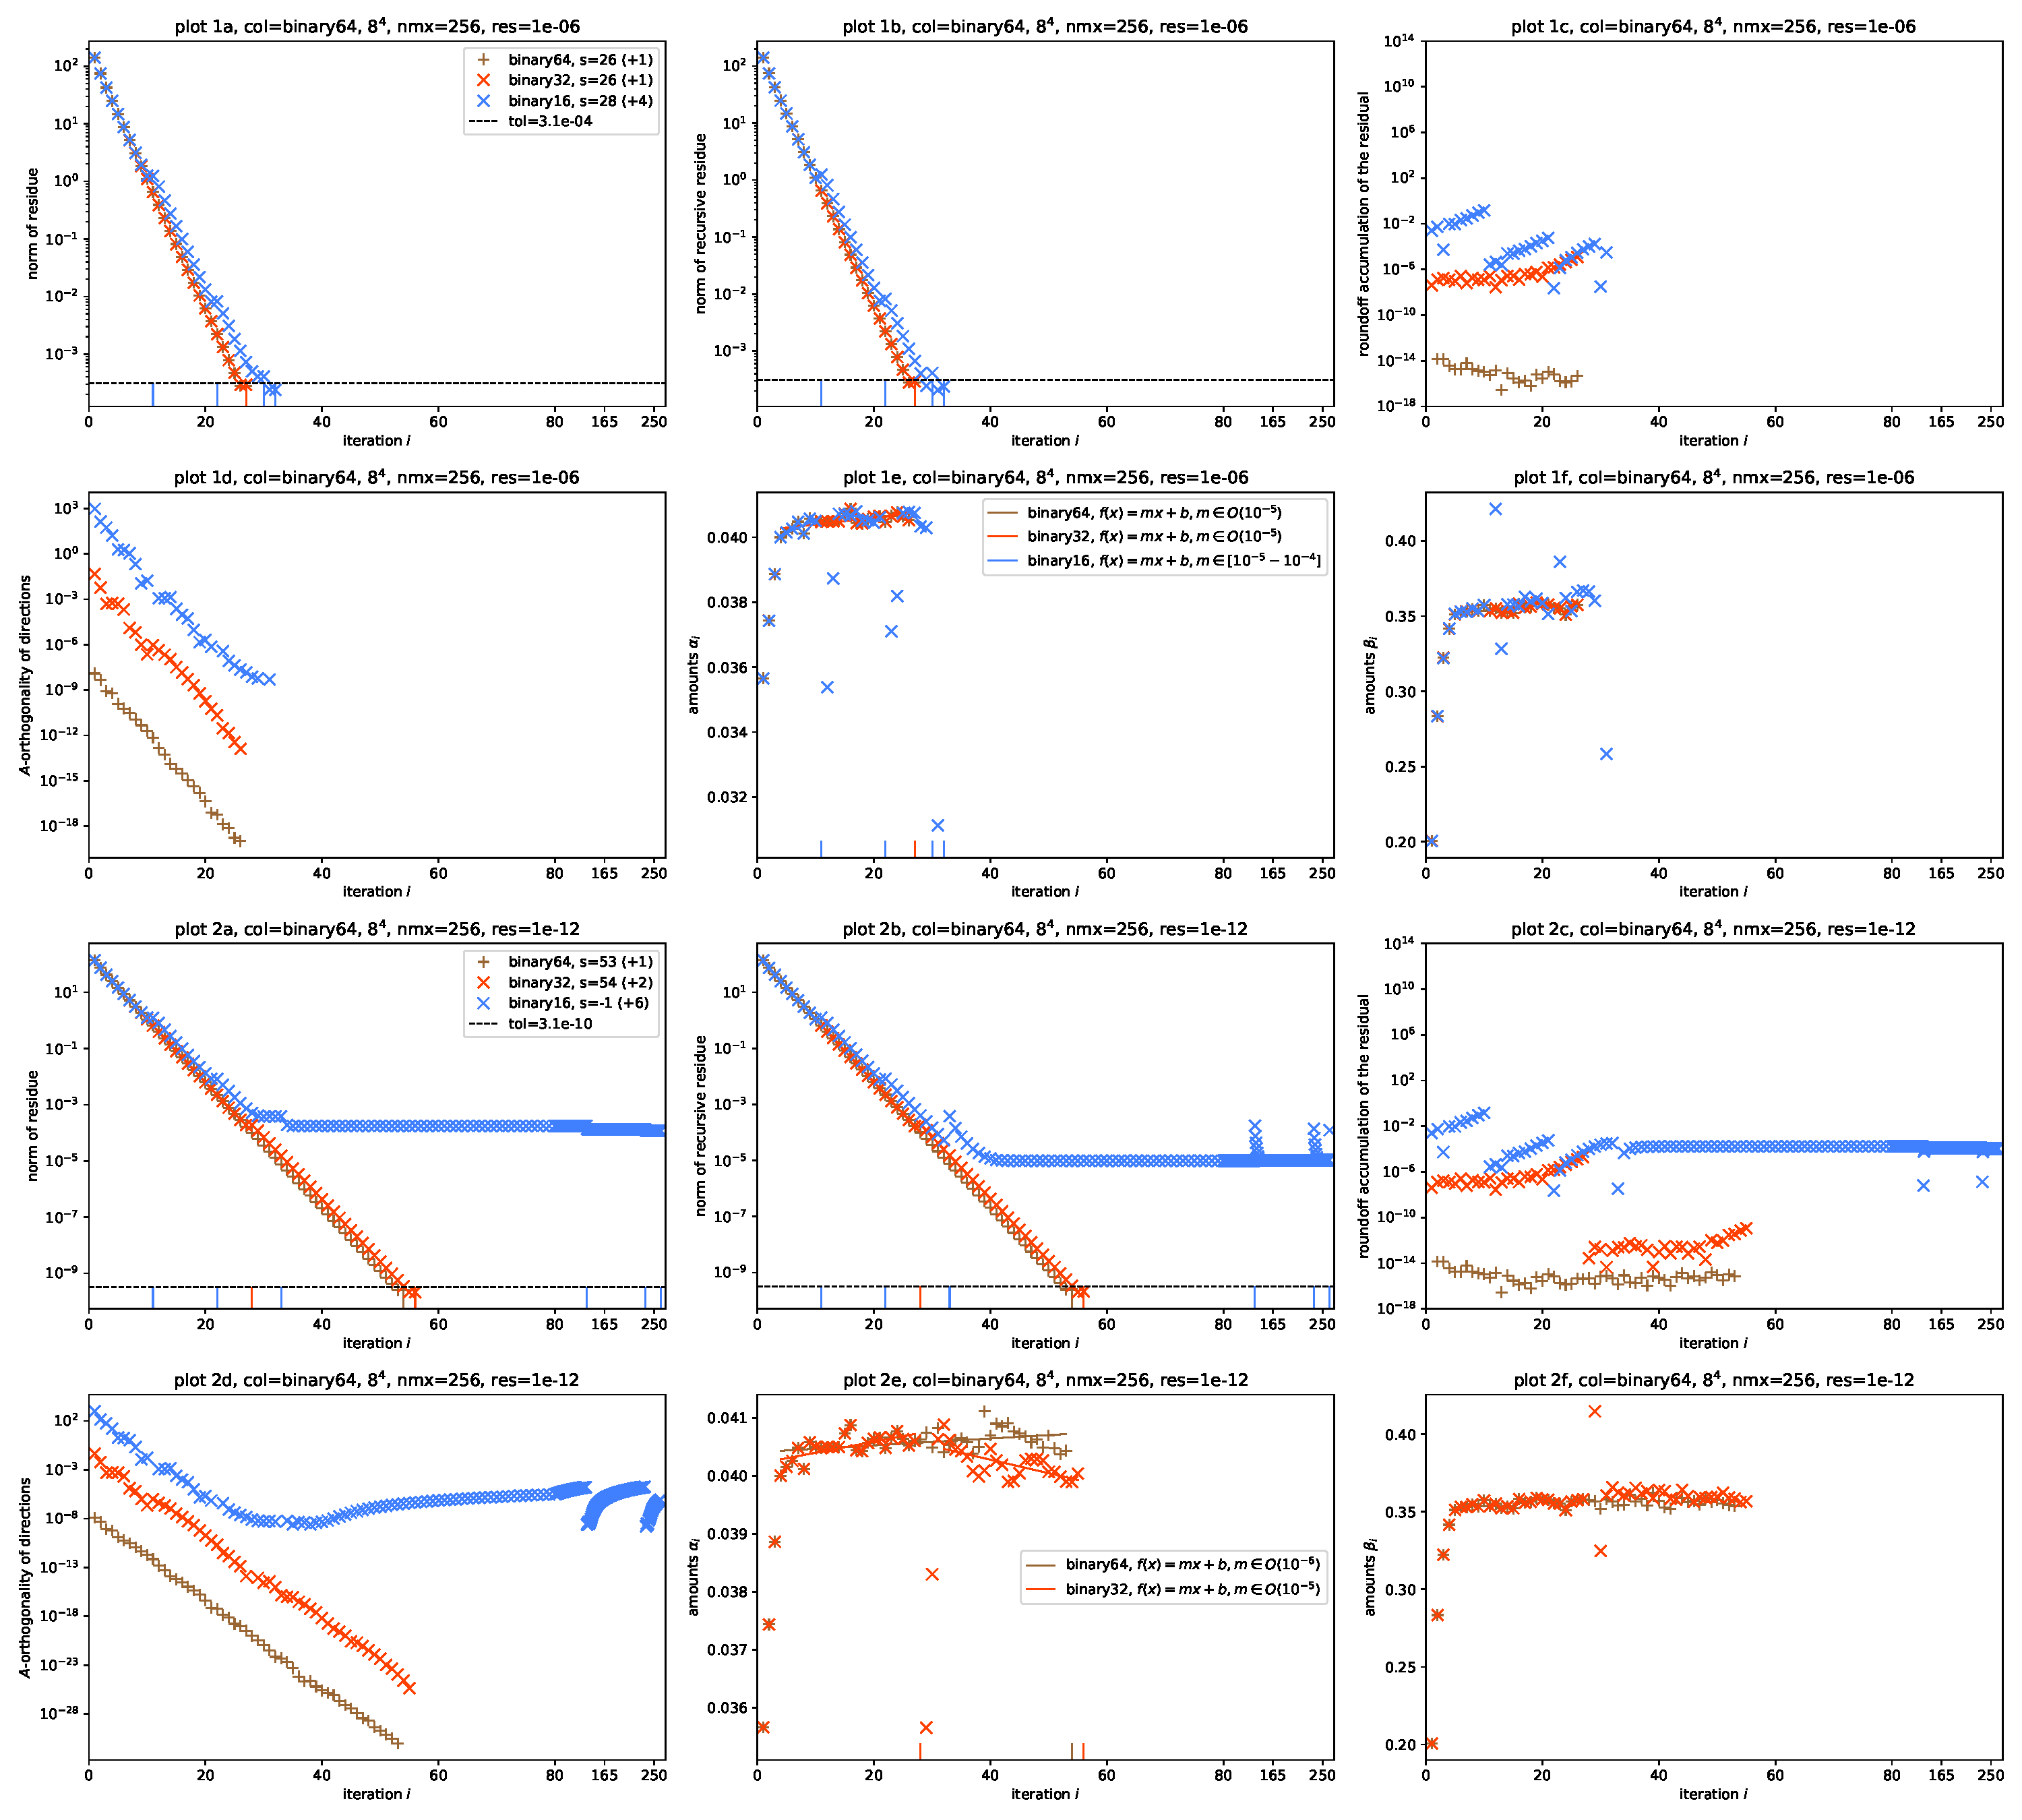
\includegraphics[width=1.0\textwidth]{plots/cgne_8x8x8x8_new}
    \caption{Analogue to figures \ref{fig:cgne:col64} and \ref{fig:cgne:res12}. This time an $8^4$ lattice was used and only the floating-point data types that are available in hardware nowadays were simulated. The \textit{first and second row} use \gls{binary64} as collective variable and $10^{-6}$ was the desired relative residual. The \textit{third and fourth row} have the same setup, but with a relative residual of $10^{-12}$ instead.}
    \label{fig:cgne8}
\end{figure}

\subsubsection{Conclusion}

The decision between floats and posits is not trivial. There is currently no hardware available, that has dedicated posit units and posits are not studied as intensive as floats. Furthermore, floats are widespread, well understood and implemented in common hardware.

%It highly depends on how fast the machine can perform \acrshort{FLOPS} and \acrshort{POPS}. For example, division in floating-point arithmetic is very expensive (it may exceed \num{24} CPU cycles, many compiler optimisations evade them), whereas in posit arithmetic it is said to be cheap, because obtaining the inverse of a number is easy.

If one decides to replace \gls{binary32} with posits, the most elegant solution would be to naively replace the data type and utilise \glspl{quire} in collective operations. To use \gls{binary64} in reduction variables is not recommended, because this would introduce many type conversions between the floating-point and the posit format which is assumed to be expensive. The drawback of this method is that \gls{posit16} may only converge if the relative residue is not chosen high enough (see plot \textit{2a} in figure \ref{fig:cgne:quire}).

If the decision goes for floats, which might be the more realistic scenario, then the most elegant solution would be to use reduction variables in \gls{binary64}. Type conversions between different IEEE floating-point types are not considered to be expensive. The \gls{tensorfloat32} compared to \gls{binary32} and \gls{bfloat16} answers the question how important precision is in the calculation. All of them have the same number of exponent bits and therefore approximately the same number range, but very different precisions. We see that all of them were able to converge in any experiment, but with \gls{binary64} as collective variable, the results were closest to each other (see figure \ref{fig:cgne:col64} plot \textit{3a}). The only relevant difference was in the number of reset steps. If the data type is lower in bit-length, the memory-boundedness suggests that the calculation performs faster, but the trade-off is the amount of (computationally expensive) reset steps that increase with decreased precision. However, the data type for reduction operations should be precise and should have a large number range. Since the number of variables needed in that data type does not scale with the problem size or the number of steps, we can use a data type with large bit-length such as \gls{binary64}. Comparing the convergence of \gls{bfloat16} in the naive case (figure \ref{fig:cgne:naive} plot \textit{1a}) with the case \gls{binary64} collective variables (figure \ref{fig:cgne:col64} plot \textit{3a}), it can be seen that the algorithm converged \num{21} steps faster, only because the reduction data type was chosen to be \gls{binary64}. On the other hand, comparing the performance of \gls{binary16} in the two plots, we see that the number range of the reduction data type brought \gls{binary16} from no convergence to convergence within \code{status=35} steps -- only marginally slower than \gls{binary32}.

These arguments make \gls{binary64} the best choice for reduction variables. Furthermore, the results show that further reducing the precision still maintains a functional solver.

\begin{proposal}{Mixed Precision Solvers}{mp}

The above analysis suggests that the calculation of the solution can (at least partially) be conducted in an even less precise data type than \gls{binary32}. One could for example choose \num{3} data types with different precision. The algorithm can be started using the least precise one. If the tolerance hits a certain value at the boundaries of the data type, the algorithm switches to the next higher one. The calculation is continued in that data type until the tolerance reaches the limits of the new data type. Again, the data type is switched to the next higher one\footnote{One obvious choice could be $d = \{\text{binary16}, \text{binary32}, \text{binary64}\}$. When the algorithm is started in \gls{binary16} and a tolerance of $\approx 10^{-4}$ is reached, the algorithm continues in \gls{binary32}, the limit of which is at a tolerance of $\approx 10^{-30}$. A continuing calculation would then be performed in \gls{binary64}.}. Calculating in mixed precision is not dependent on the algorithm itself and can therefore be applied to every iterative solver.

Algorithm \ref{alg:mixed_precision} shows an example implementation of such a mixed precision calculation. The array $d$ consists of all available data types participating in the calculation in ascending order, meaning the least precise data type comes first. The function $solve()$ performs the underlying algorithm (for example conjugate gradient) in the data type given by its arguments. It expects at least a starting vector $\vec{x_0}$ and a tolerance and returns the status\footnote{See section \ref{sec:fp_in_openqxd}}, the calculated solution and the residual up to the given tolerance. Reduction variables within $solve()$ are calculated in a datatype with high precision.

\end{proposal}

\begin{figure}
\centering
\begin{minipage}{.6\linewidth}
\begin{algorithm}[H]
\SetKwInOut{Input}{input}
\Input{desired norm of relative residual $rn$}
\Input{array of data types in $\{d\}_{k=0}^N$}
\Input{iterative algorithm $solve()$}
\SetAlgoLined
  $\vec{x_0}, \vec{r_0}, \ldots \gets$ initial guess, \ldots\;
  $\vec{x}, \vec{r} \gets \vec{x_0}, \vec{r_0}$\;
  status $\gets 0$\;
  \For{$k \gets 0, 1$ \KwTo $N$}{
    convert all variables to data type $d[k]$\;
    $tol \gets \frac{1}{\norm{\vec{r_0}}} max(rn, \text{\code{MACHINE\_EPSILON of $d[k]$}})$\;
    substatus, $\vec{x}, \vec{r}$, $\ldots \gets solve(tol, \vec{x}, \ldots)$\;
    \uIf{substatus $> 0$}{
      status $\gets$ status $+$ substatus\;
    }
    \uIf{$\norm{\vec{r}} < rn$}{
      \Return status, $\vec{x};$ \tcp{success}
    }
 }
 status $\gets -3$\;
 \Return status, $\vec{x_0};$ \tcp{the algorithm failed}
 \caption{Pseudo-code for an iterative algorithm in mixed precision.}
 \label{alg:mixed_precision}
\end{algorithm}
\end{minipage}
\end{figure}

\begin{proposal}{Approximating the amounts $\alpha_i$}{alpha}

Looking at plot \textit{4e} of figure \ref{fig:cgne:res12}, where the amounts $\alpha_i$ are plotted for every iteration, we see that after every reset step the amounts need $2-3$ steps to reach a value that is not changing very much for future iterations. This becomes apparent when looking at the fitting lines. The values of the $\alpha_i$ are in the range $10^{-1}$ and the slopes $m$ of the fitting lines are in the range $10^{-4}$ - $10^{-5}$, suggesting that the value of $\alpha_i$ is not changing from iteration to iteration when only looking at $2-3$ significant decimal digits.

A possibility to reduce computational cost in each iteration could be to approximate the values of future $\alpha_i$ to be constant. The less precise the data type, the larger the change in $\alpha_i$. The large error in $\alpha_i$ of \gls{bfloat16} in all plots suggests that the algorithm is not sensible to errors in $\alpha_i$. Therefore, it can be expected that the results should not change significantly with an approximated value of $\alpha_i$.

\begin{itemize}
    \item Advantage: The residuals can be calculated using $\vec{b} - A \vec{x}$, instead of recursively. This implies less round-off accumulation.
    \item Advantage: Only one matrix-vector multiplication per iteration.
    \item Disadvantage: Since the $\alpha_i$ are just approximated, the number of required iterations may increase.
    \item Disadvantage: The Dirac-operator $D$ must be given in the form of $A = D^{\dagger} D$ as \textit{one} operator, else the algorithm still consists of \num{2} matrix-vector multiplications per iteration and the benefit is non-existent. Also, $D^{\dagger} D$ is less sparse than $D$.
\end{itemize}

The results of simulations with approximated values for the $\alpha_i$ can be observed in plot series \ref{fig:cgne:4x4x4x4:e1} and \ref{fig:cgne:8x8x8x8:e1}. The value was approximated based on previous values. The first \num{5} steps where skipped (thus the algorithm performed natively). In step number \num{5}, the last \num{3} values of $\alpha_i$ where averaged. In the following steps the constant value calculated in step \num{5} was reused. After every reset step, the value of $\alpha_i$ had to be recalculated using the above procedure. Therefore, a data type such as \gls{bfloat16} that has reset steps after approximately every \num{7}th regular step, will benefit in only \num{2} steps per reset step. This is little difference to native runs of data types with high precision.

The calculation became more sensible to the number range of the data type. This can be seen in all plots when looking at \gls{binary16} that was not able to converge anymore, although by a very small amount. \Gls{tensorfloat32} on the other hand performed similar to the regular rounds, it was expected that it needs slightly more iterations. When going with this strategy, it is therefore advisable to perform more regular CG-steps when coming closer to the boundaries of the data type. One possible solution would be to choose a higher machine epsilon close to the boundaries, forcing the algorithm to perform more reset steps, in turn causing more regular CG-steps and recalculations of $\alpha_i$.

Notice that with larger lattice sizes, the approximation of the amounts has less error (see plots \textit{1e} and \textit{2e} in figures \ref{fig:cgne:4x4x4x4:e1} and \ref{fig:cgne:8x8x8x8:e1}) and the algorithm is thus more stable.

\end{proposal}

\begin{figure}
    \centering
    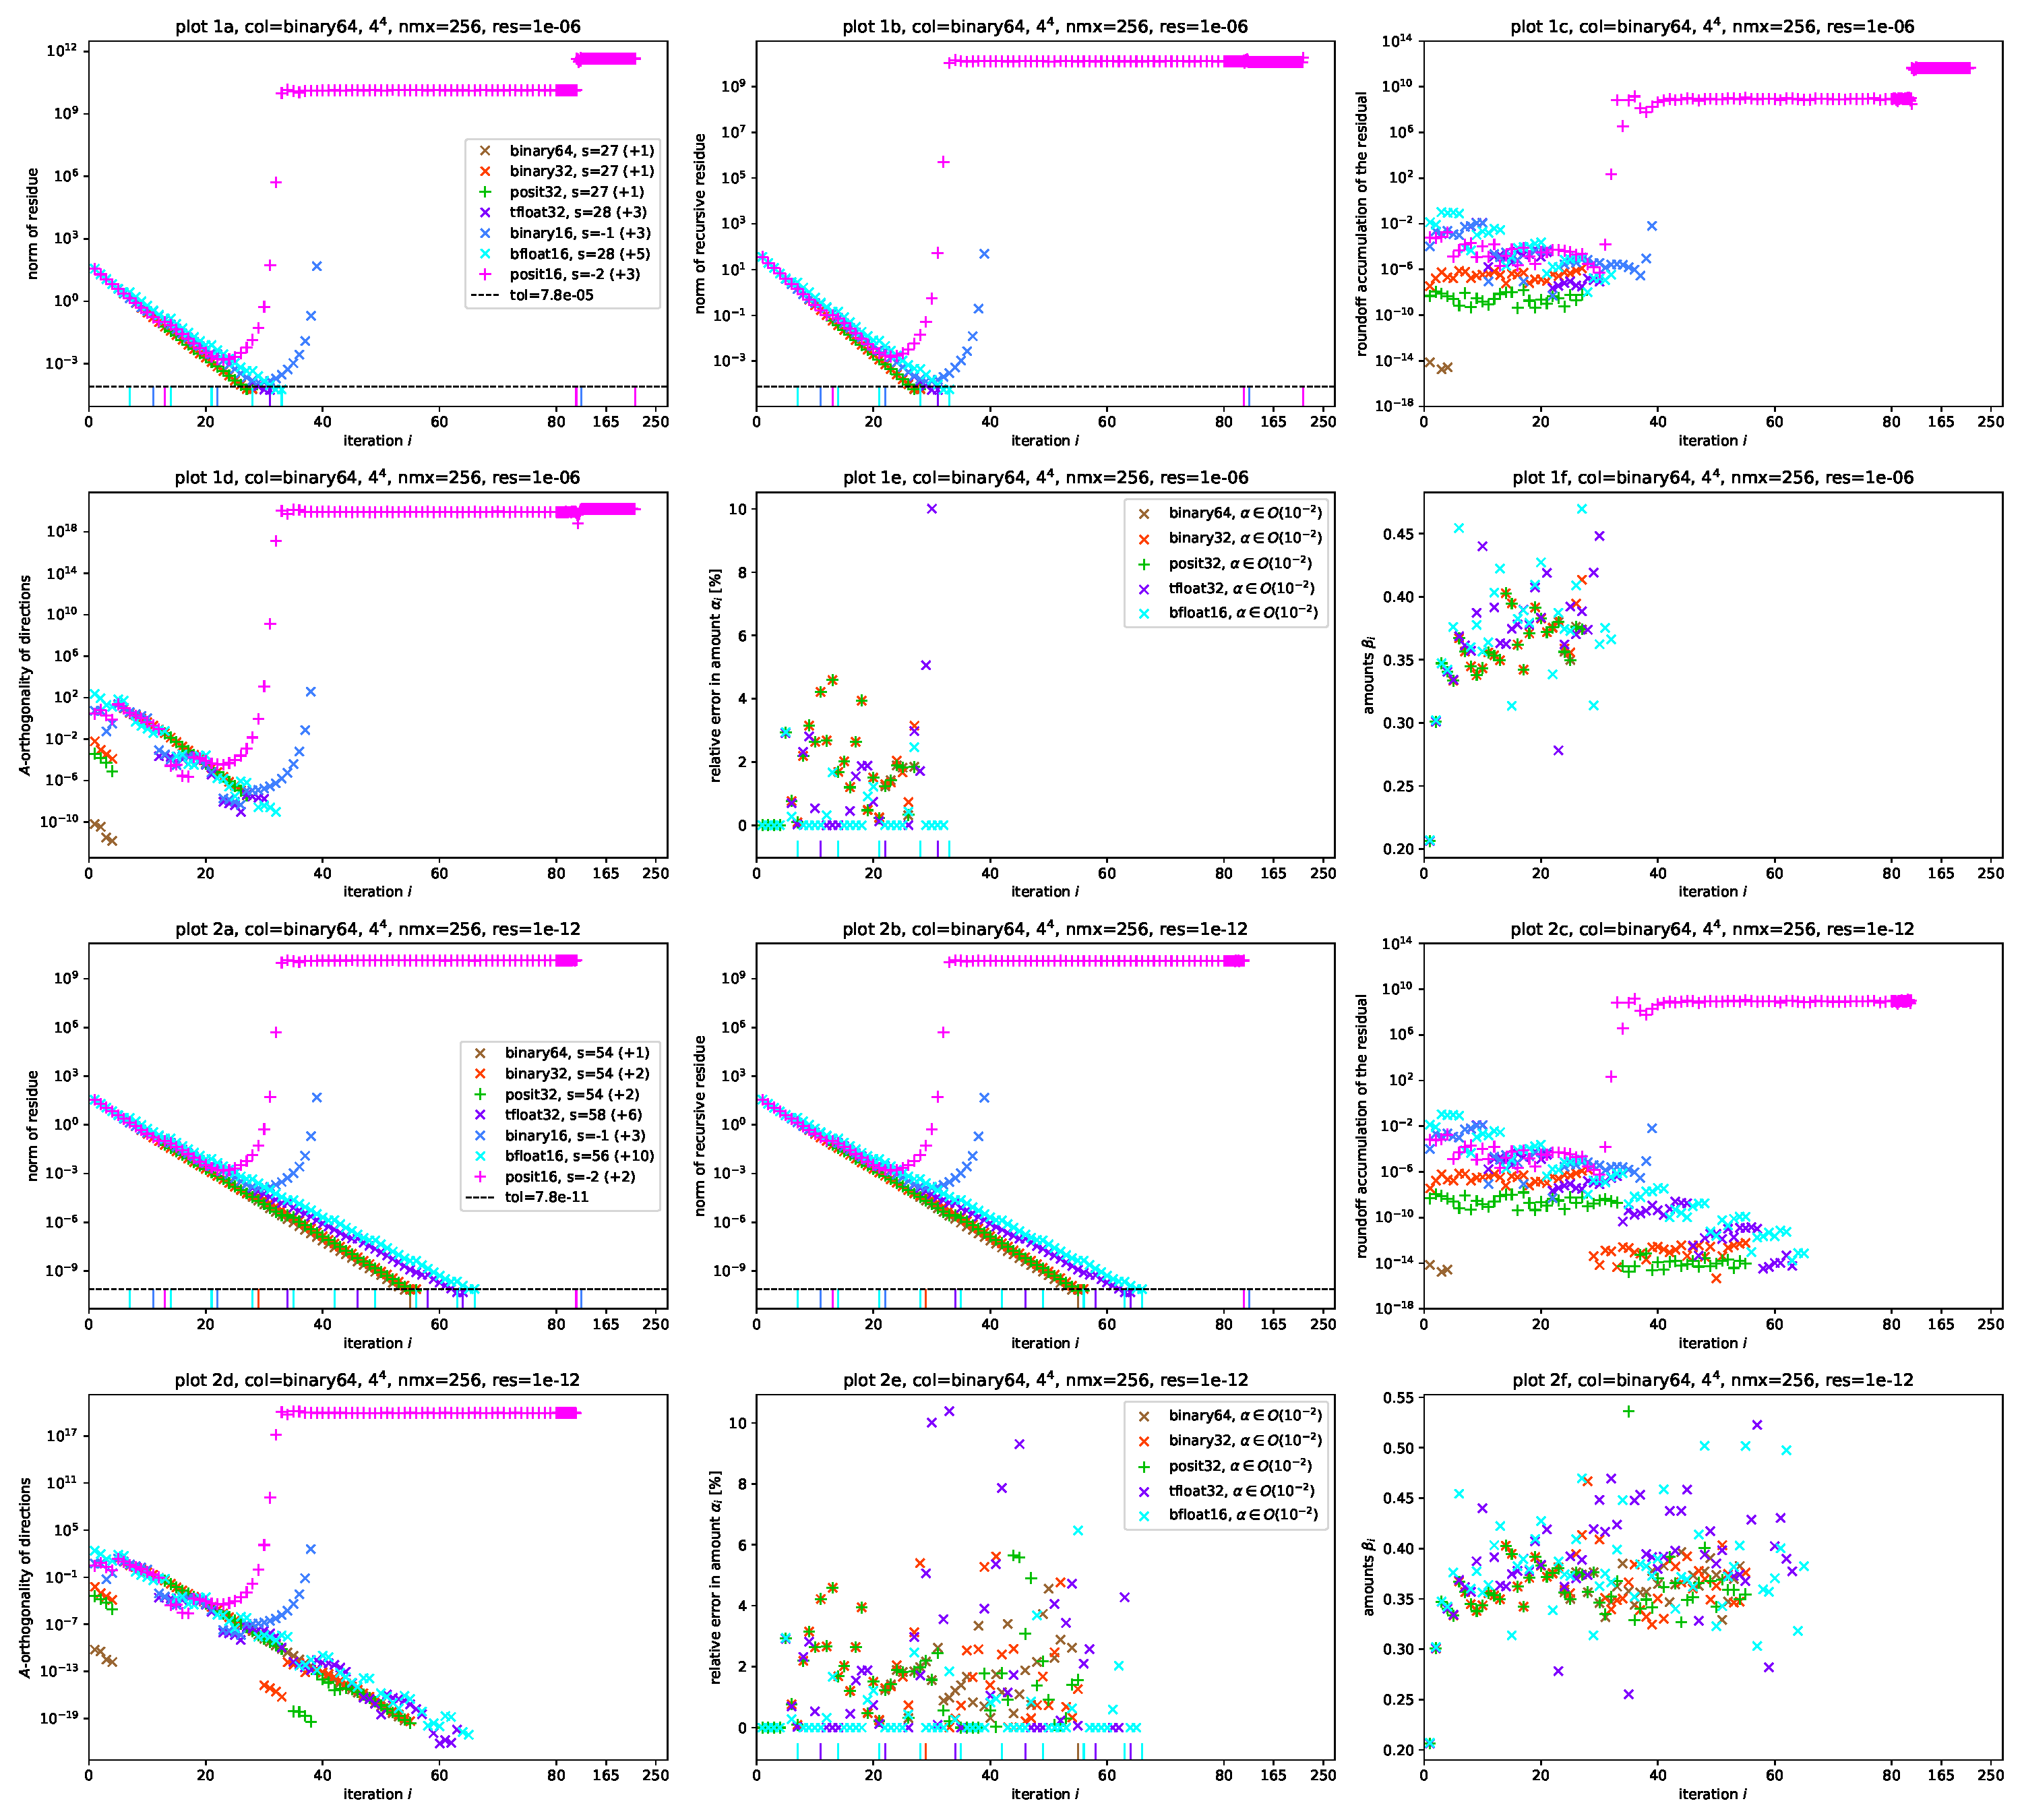
\includegraphics[width=1.0\textwidth]{plots/cgne_4x4x4x4_e1}
    \caption{Plots \textit{1a} to \textit{1f} shows the convergence analysis of a conjugate gradient run with a $4^4$ lattice, relative residual $10^{-6}$ and approximated values of $\alpha_i$. In plots \textit{2a} to \textit{2f} the residual was chosen to be $10^{-12}$. Plots \textit{1e} and \textit{2e} show the relative error in the approximated $\alpha_i$ compared to the real $\alpha_i$.}
    \label{fig:cgne:4x4x4x4:e1}
\end{figure}

\begin{figure}[h]
    \centering
    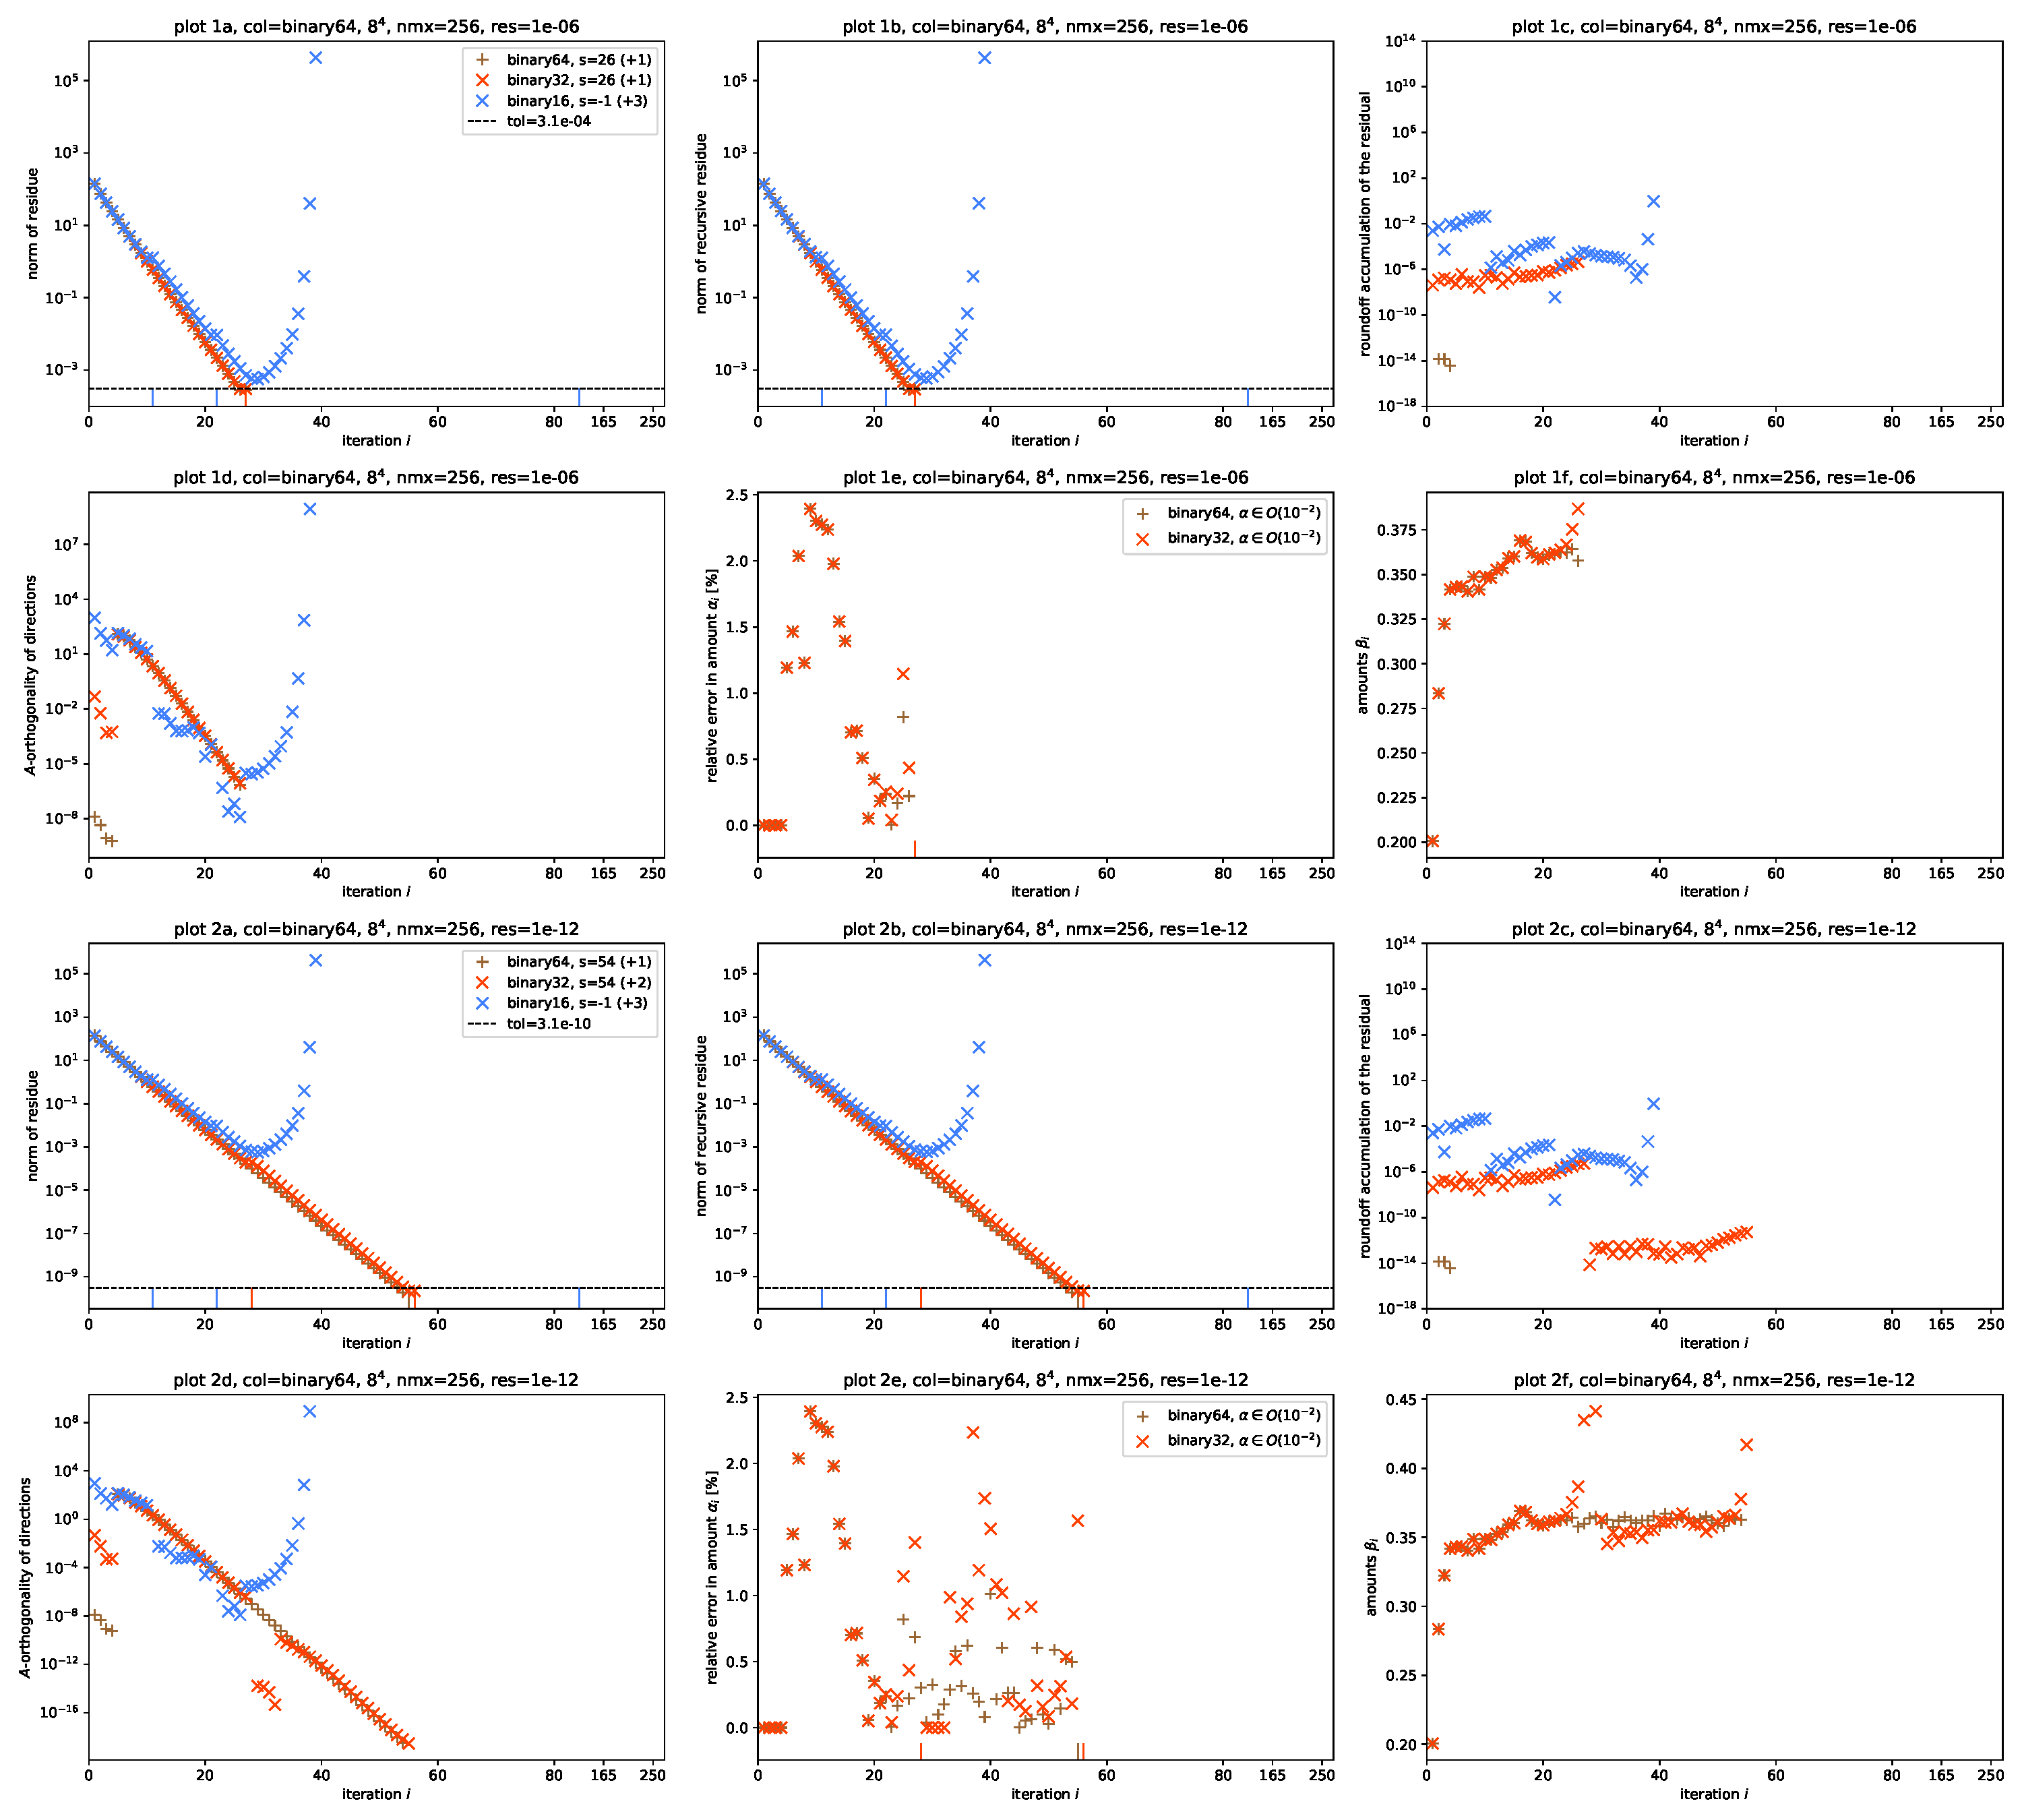
\includegraphics[width=1.0\textwidth]{plots/cgne_8x8x8x8_e1}
    \caption{The same setup as figure \ref{fig:cgne:4x4x4x4:e1}, but with an $8^4$ lattice.}
    \label{fig:cgne:8x8x8x8:e1}
\end{figure}

\begin{comment}

res $> 10^{-6}$

Simulated data type: precision $>$ number range

Collective data type: number range $>$ precision

res $< 10^{-6}$

Simulated data type: precision $>$ number range

Collective data type: number range $>$ precision

\end{comment}

\section{SAP preconditioned GCR}

\label{sec:sap_gcr}

To study spontaneous chiral symmetry breaking we need large lattices and small masses. Conjugate gradient and related algorithms become inefficient on such lattices. The lattice Dirac-operator gets increasingly ill-conditioned in such setups. The solver presented in the following is called \acrshort{sapgcr}. It makes use of a multiplicative \acrfull{sap} as preconditioner for a flexible \acrfull{gcr} solver. Parallelizing the algorithm is straight forward, because it consists of decomposing the large problem into many smaller independent ones.

\subsection{Even-Odd Preconditioning}

Preconditioning in general, when employed in lattice QCD, is expected to have significant impact on the number of iterations of a solver. One way of preconditioning $D \psi = \eta$ on a lattice is

\begin{align*}
    L D R \psi^{\prime} = L \eta,
\end{align*}

with $\psi = R^{-1} \psi^{\prime}$ and $L$, $R$ chosen wisely such that $LDR$ is well conditioned. If $L = \mathbb{I}$, it is called \df{right preconditioning}, if $R=\mathbb{I}$ it is called \df{left preconditioning}. If the Dirac-matrix involves only nearest-neighbour interactions, it is possible to split the lattice into even and odd sites\footnotemark
\footnotetext{It is therefore similar to a domain decomposition method, see section \ref{sec:ddecomp}.}
\footnotemark.
\footnotetext{Even lattice points are the ones where the sum of the global Cartesian coordinates $(n_0 + n_1 + n_2 + n_3)$ in units of the lattice spacing $a$ is even, notice $x_{\mu} = a n_{\mu}$, where ${\mu} = 0, 1, \dots, D$.}
If the sites are ordered such that the even sites come first\footnotemark,
\footnotetext{This is indeed the case in openQ*D (see \code{main/README.global}) in \cite{openqxd}.}

\begin{align*}
    D &=
    \begin{pmatrix}
    D_{ee} & D_{eo} \\
    D_{oe} & D_{oo}
    \end{pmatrix},
    & & &
    \psi &=
    \begin{pmatrix}
    \psi_e \\
    \psi_o 
    \end{pmatrix}
\end{align*}

$D_{ee}$ ($D_{oo}$) consists of the interactions of the even (odd) sites among themselves, while $D_{eo}$ and $D_{oe}$ consider the interactions of even with odd sites. $\psi_e$ and $\psi_o$ contain the values for even and odd lattice sites of the spinor.

Using specific forms of $L$ and $R$, $D$ can be brought into a block-diagonal form, namely

\begin{align*}
    L &= 
        \begin{pmatrix}
        1 & -D_{eo} D_{oo}^{-1} D_{oe} \\
        0 & 1
        \end{pmatrix}
    & &\text{and} &
    R &= 
        \begin{pmatrix}
        1 & 0 \\
        -D_{oo}^{-1} D_{oe} & 1
        \end{pmatrix}.
\end{align*}

After a bit of algebra,

\begin{align*}
    L D R &= 
        \begin{pmatrix}
        \hat{D} & 0 \\
        0 & D_{oo}
        \end{pmatrix},
    & &\text{with} &
    \hat{D} &= D_{ee} - D_{eo} D_{oo}^{-1} D_{oe}.
\end{align*}

This specific preconditioning reduces the amount of iterative steps needed by a factor of \num{2} approximately, because $D_{oo}$ and $\hat{D}$ are matrices of half the dimension of $D$. The inversion of $D_{oo}$ is simple, because with only nearest-neighbour-interactions the odd sites do not interact among themselves, only with even sites. Thus $D_{oo}$ exhibits block-diagonal form (all blocks are $6 \times 6$). Using

\begin{align*}
    D \psi = \eta \implies \begin{pmatrix}
    D_{ee} & D_{eo} \\
    D_{oe} & D_{oo}
    \end{pmatrix} \begin{pmatrix} \psi_e \\ \psi_o \end{pmatrix} = \begin{pmatrix} D_{ee} \psi_e + D_{eo} \psi_o \\ D_{oe}\psi_e + D_{oo} \psi_o \end{pmatrix} = \begin{pmatrix} \eta_e \\ \eta_o \end{pmatrix},
\end{align*}

we can write the preconditioned form, where only the reduced system with even lattice sites has to be solved to determine $\psi_e$,

\begin{align*}
    \hat{D} \psi_e &= D_{ee} \psi_e - D_{eo} D_{oo}^{-1} D_{oe} \psi_e \\
    &= ( \eta_e - D_{eo} \psi_o ) - D_{eo} D_{oo}^{-1} ( \eta_o - D_{oo} \psi_o ) \\
    &= \eta_e - D_{eo} D_{oo}^{-1} \eta_o,
\end{align*}

because $\psi_o$ follows from the solution $\psi_e$ via

\begin{align*}
    \psi_o = D_{oo}^{-1} (\eta_o - D_{oe} \psi_e).
\end{align*}

\begin{remark}
Note that it works only because $D_{ee}$ is diagonal in space for Wilson (and Wilson-twisted) fermions.
\end{remark}

\begin{remark}
This preconditioning method does not allow multisolvers\footnote{Algorithms which solve for multiple masses in one shot, for example \acrshort{mscg}.}.
\end{remark}

\subsection{Schwarz Alternating Procedure}

\label{sec:ddecomp}

Domain decomposition is a way to partition the large system into (possibly many) smaller sub-problems with regularly updated boundary conditions coming from solutions of neighbouring sub-problems. They fit well into the notion of parallel processing because the sub-problem can be chosen to be contained in one single rank. The full lattice is split into sub-lattices called \df{local lattice}. Each rank has its own local lattice, the size of which is determined at compilation time. The full lattice consists of the ensemble of all local lattices arranged in a grid. It is therefore advisable to choose the size of the decomposed sub-domains as divisor of the local lattice size such that one or more blocks fit into one rank. These sub-problems can then be solved using an iterative solving method.

\begin{figure}[h]
  \centering
  %\includestandalone[]{schemes/domain_decomposition}
  \subimport{schemes/}{domain_decomposition}
  \caption{A $d=2$ dimensional example of a decomposition of a lattice $\Omega = \bigcup_{i=1}^{n} \Omega_i$ into $n=16$ domains named $\Omega_i$. Notice such a decomposition can always be colored like a chessboard.}
  \label{fig:ddecomp}
\end{figure}

The idea behind \acrlong{sap} is to loop through all blocks $\Omega_i$ and solve the smaller sub-problem using boundary conditions given from the most recent global solution (see figure \ref{fig:ddecomp}). If the original problem only includes nearest-neighbour interactions, the solution of a block $\Omega_i$ depends only on that block and its exterior boundary points, which are the adjacent points on the neighbouring blocks with opposite color. For example, the solution of the sub-problem involving $\Omega_6$, depends only on the solutions of $\Omega_2$, $\Omega_5$, $\Omega_7$ and $\Omega_{10}$\footnotemark.
\footnotetext{It depends on all other sub-problems as well, but indirectly.}
Therefore, all grey (white) sub-problems can be solved simultaneously, with the most recent boundary conditions obtained from the white (grey) domains. Solving all grey, followed by all white sub-problems is called a \df{Schwarz-cycle} and is considered one iteration in \acrshort{sap}. Each sub-problem can be solved with any desired solver separately, again applying some preconditioning\footnotemark.
\footnotetext{Using even-odd preconditioning is perfectly fine with $D$ replaced by the restricted Dirac-operator $D_i$ acting only on the points in $\Omega_i$.}

\begin{figure}[h]
    \centering
    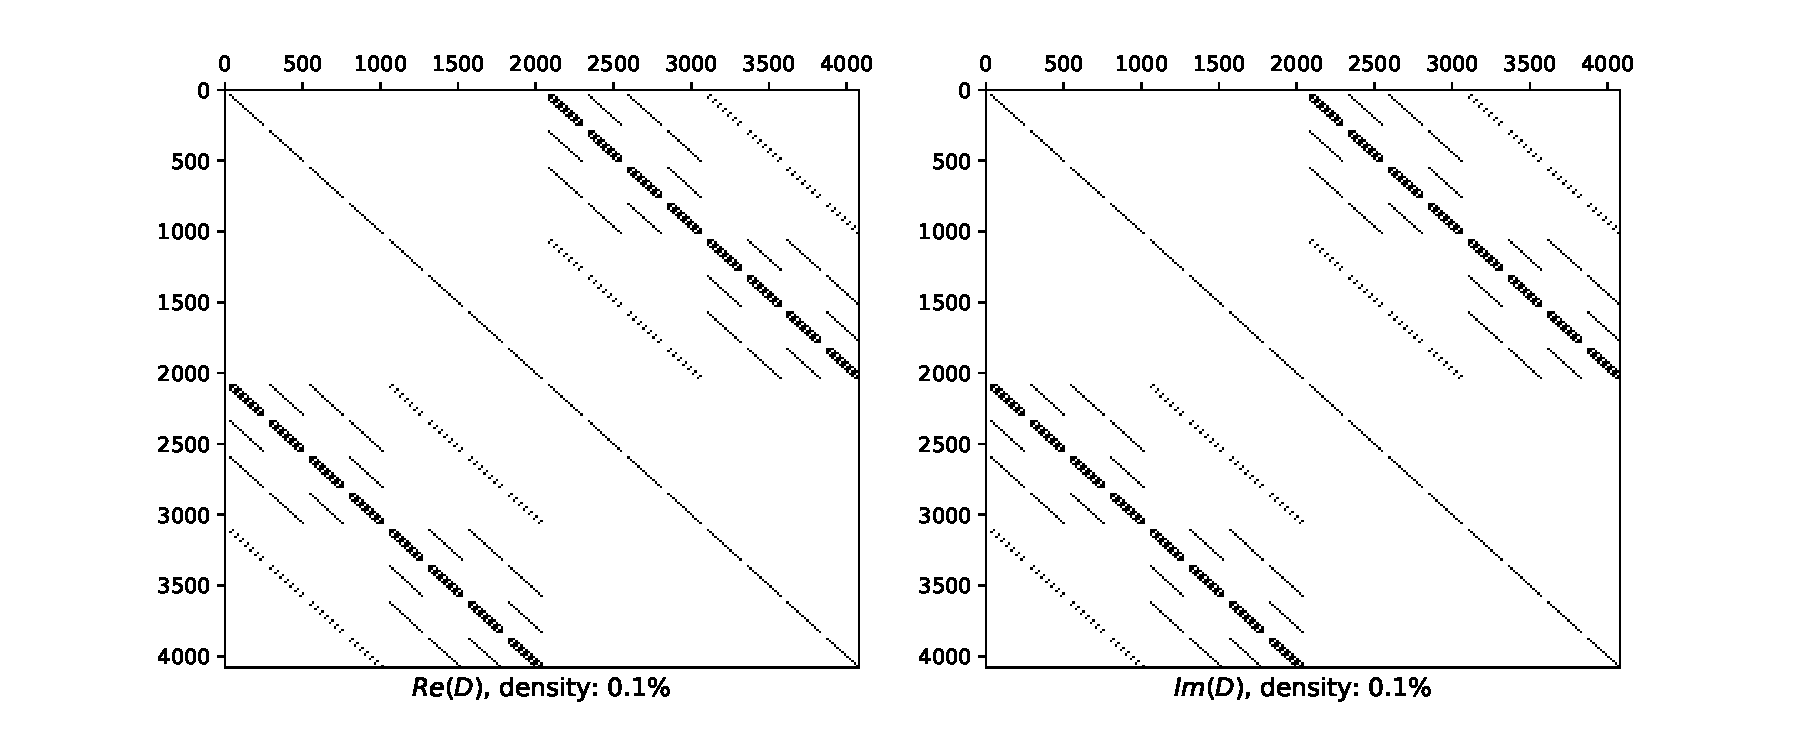
\includegraphics[width=1.0\textwidth]{plots/dirac_matrix6}
    \caption{An example plot of a Dirac-matrix of an $8^4$-lattice with \acrshort{sf}-boundary conditions. The operator is already in a shape, where the even lattice points come first, followed by the odd lattice points. Every pixel consists of $192 \times 192$ real numbers. If the average over that numbers is non-zero the pixel is drawn black, else the pixel is drawn white. The density gives the overall percentage of non-zero values.}
    \label{fig:dirac_matrix}
\end{figure}

Whereas the division into domains on the lattice is straightforward, the representation of the Dirac-operator as a sparse matrix and its decomposition is not. Looking at an actual example of a Dirac-operator written as a matrix (see figure \ref{fig:dirac_matrix}), one observes a lot of structure: while on the diagonal we find the operators restricted to the black and white blocks, the first and the third quadrant describe the operators restricted to the interior and exterior boundaries. The operator restricted to the exterior boundaries of the union of all black (white) blocks is denoted by $D_{\partial b}$ ($D_{\partial w}$). The decomposition into $2n$ domains ($n$ grey and $n$ white blocks) can be translated as seen in figure \ref{fig:ddecomp_matrix}. Notice that the restricted operators $D_i$ are well-conditioned because they have block diagonal form. The blocked problem would then look like, $i = 1, \dots, 2n$,

\begin{align*}
    D_i \psi_i = \eta_i.
\end{align*}

\begin{figure}[h]
  \centering
  %\includestandalone[]{schemes/dd_matrix}
  \subimport{schemes/}{dd_matrix}
  \caption{Schematic of the Dirac-operator in terms of a large sparse matrix. If the components of the black blocks are arranged such that they appear first, then the decomposition from figure \ref{fig:ddecomp} can be translated into a matrix with blocks as in the picture. $D_i$ describes the Dirac-operator restricted to block $i$ and $D_{\partial b}$ ($D_{\partial w}$) is the Dirac-operator restricted to the external boundaries of the black (white) blocks. The color external boundary operators can be decomposed into external boundary operators of the $i$-th block, $D_{\partial^{*}_i}$. The right side describes a vector decomposed into the same $2n$ domains $\psi_1, \dots, \psi_{2n}$. The upper half corresponds to the black blocks and the lower half to the white blocks.}
  \label{fig:ddecomp_matrix}
\end{figure}


\begin{comment}
TODO: formulate the block sub-problem here, and the sap cycle. D only couples nearest-neighbour blocks, see (0706.2298 Local coherence and deflation of the low quark modes in lattice QCD Fig.4)

kappa, the lattice hopping term, determines to how many neighbours the interactions are extended.
the wilson dirac operator D_w in doc/dirac.pdf eq (10) has only nearest neighbour interactions
\end{comment}

\subsection{SAP as a Preconditioner}

\begin{comment}

No overlapping (why?) of domains, as preconditioner (why?)

Before calling GCR, calculate the P_i and T_i (Saad Page 490), i-th operator for i-th rank.
Then calc M^-1 b using the T_i simultaneously on all ranks
Start GCR
In each GCR step: M^-1 A x_i must be calculated, using the P_i on all ranks simultaneously.
M^-1 is the preconditioner that is not explicitly available, only implicitly via the P_i. However the M^-1 is not an exact inverse of A, but approximates A^-1. The remaining matrix B = M^-1 A is "close" to the identity, which makes Bx=c solved in very few steps, with c=M^-1b.

The domain decomposition preconditioner based on \acrshort{sap} involves itself an iterative procedure and is therefore very expensive.

* fixed number of GMRES iterations can be a preconditioner as well
* choice of preconditioner is often more important than the choice of iterative method [Yousef Saad book]
* preconditioning = bringing the condition number of a matrix closer to 1 (cond(id) = 1)

The block sizes bs[4] and other parameters of the specified block grid
are obtained from the parameter data base. These and the lattice sizes
must be such that the lattice can be covered by non-overlapping blocks.
Moreover, the number of blocks in each direction must be even and the
local lattices must contain an even number of blocks. This ensures that
the block grid can be chessboard-coloured and that the number of blocks
in the local lattice is the same for both colours.

The blocks are ordered such that the first half of them have the same colour (black by definition).

\end{comment}

The multiplicative \acrlong{sap} is a domain decomposition method coming from the theory of partial differential equations. It can be applied in the form of a right preconditioner $M^{-1}$ making the preconditioned system

\begin{align}
    M^{-1} A \vec{x} = M^{-1} \vec{b} \label{eq:sap:preconditioned}
\end{align}

to be solved in very few steps, if $M^{-1}$ is a good approximation for $A^{-1}$. The preconditioning matrix $M^{-1}$ is never explicitly available during the calculation, such as it is the case in even-odd preconditioning which can also be applied in advance. To solve the preconditioned equation \eqref{eq:sap:preconditioned} using an iterative Krylov subspace method\footnote{such as \acrlong{cg}, \acrlong{gmres}, \acrlong{mr}, \acrlong{bicgstab} or \acrlong{gcr}.}, the algorithm must be able to apply $M^{-1}$ and $M^{-1} A$ to an arbitrary vector $\vec{v}$. If it is possible to implement such operations on multiple ranks in an efficient way and if the preconditioner makes $M^{-1} A$ well-conditioned, we reached the goal. Obviously, an application of $M^{-1}$ should be possible without involving $A^{-1}$. The actions of operators $M^{-1}$ and $M^{-1} A$ on a vector $\vec{v}$ are assembled using a multiplicative \acrlong{sap}, where the blocks are treated by some fixed number of \acrfull{mr} steps\footnotemark. The blocks need not to be solved to a certain precision, because the procedure is only used as a preconditioner approximating the solution.

%This is a motivation for proposal \ref{pp:sap_reduced_precision}.

\footnotetext{Determined by the value of \code{mnr} in the solver section of the input file.}

In openQ*D the \code{SAP\_GCR} solver is implemented as follows: The large problem is solved using a flexible \acrshort{gcr} solver, that in each of its \code{nmx} steps uses a different preconditioner. The preconditioner is given by \code{ncy} steps of the \acrlong{sap} applied to the current solution vector. Each \acrshort{sap} cycle involves approximately solving all grey blocks followed by all white blocks on the entire lattice, each with \code{nmr} steps of the \acrshort{mr} method using even-odd preconditioning (\code{isolv=1}) or not (\code{isolv=0}).

\begin{comment}
\begin{proposal}{MR in reduced precision}{sap_reduced_precision}

%\label{pp:sap_reduced_precision}
%TODO probably remove

Since \acrshort{mr} is memory-bound, it can be conducted in mixed or reduced precision.

%TODO: sap as preconditioner does not have to be precise, only approximation, thus reduced precision in the calculations? Is sap-preconditioning memory-bound? Involves network communication as well on the surface, therefore surface to volume ratio should be as small as possible, meaning the SAP-blocks should be as large as possible. Trade-off: reduced precision performs better with small blocks, but network communication is minimised with large blocks.
EO-reconditioning also in reduced precision?

\end{proposal}

\end{comment}

\begin{proposal}{Performing MR steps on the GPU}{sap_mr_gpu}

The preconditioning procedure involves \code{mnr} \acrshort{mr} steps to be taken on each block in each Schwarz-cycle to approximate a solution to the block problem. Since blocks of the same color are independent of each other and the Dirac-operator acting only on a specific block involves no communication whatsoever, we can conclude that the procedure of solving a sub-problem is \textit{local} to the block and self-contained in the sense that it can be solved independently and without MPI communication among ranks. This could be a very handy starting point when going towards GPU-utilisation.

Once the source vector and the restricted Dirac-operator are transferred to the GPU (both stay constant during the solving process), the problem can be solved on the GPU without involving any communication with other ranks or GPUs. This can be beneficial, because of the following argument: the local lattice of one single rank, can be subdivided into multiple blocks as well (imagine figure \ref{fig:ddecomp} being the local lattice). The actual implementation solves the grey (white) blocks in a local lattice sequentially\footnote{By iterating over the blocks, see \code{sap()} at line \num{717}ff in \code{modules/sap/sap.c} in \cite{openqxd}.}. Since all the grey (white) problems within the local lattice can be solved simultaneously, the code does not exploit the full concurrency potential of the procedure. Solving the sub-problems on the GPU, one could launch \acrshort{mr} solvers on all grey blocks simultaneously followed by all white blocks. The \acrshort{mr} solver can be called in mixed or even reduced precision.

For a specific implementation of the GPU-solver, one possibility is to encode the restricted Dirac-operator in one of the sparse matrix formats (for example \acrshort{csr}) and use already existing libraries (for example \cite{bell2008} for \acrshort{cuda}) for an application to a spinor. The results in section \ref{sec:sap_gcr_results} are obtained using such an approach.

Comparing the implementation of the Dirac-operator in QUDA (see ref. \cite{clark2010}), it is advisable to not rely on such generic libraries, because they ignore further symmetries and structure of the operator. The problem lies mostly in the memory-boundedness of the procedure.

\end{proposal}

\subsection{Generalised Conjugate Residual}

The choice for the outer solver goes to \acrshort{gcr}, because inexact preconditioning is then possible without affecting the correctness of the solution \cite{luscher2004,luscher2007}.

We wish to solve \eqref{eq:Axb} if $A$ is not Hermitian. Comparing to the conjugate gradient algorithm, we minimise the residual $\vec{r}$ of the solution $\vec{x}$, using the \df{quadratic form}

\begin{align*}
    f(\vec{x}) &= \frac{1}{2} \left( \vec{b} - A \vec{x} \right)^{\dagger} \left( \vec{b} - A \vec{x} \right) + c \\
               &= \frac{1}{2} \norm{ \vec{b} - A \vec{x} }^2 + c\\
               &= \frac{1}{2} \norm{ \vec{r} }^2 + c,
\end{align*}

where $c \in \mathbb{C}$. When taking the derivative of this function with respect to $\vec{x}$, we find that

\begin{align*}
    f'(\vec{x}) = A^{\dagger} A \vec{x} - A^{\dagger} \vec{b}.
\end{align*}

\begin{lemma}[Uniqueness of the solution]
The solution $\vec{x}$ in equation \eqref{eq:Axb} is unique and the global minimum of $f(\vec{x})$, if $A$ is non-singular.
\end{lemma}

\begin{proof}
Let us rewrite $f(\vec{p})$ at an arbitrary point $\vec{p} \in \mathbb{C}$ in terms of the solution vector $\vec{x}$,

\begin{align*}
    f(\vec{p}) &= \frac{1}{2} \left( \vec{b} - A \vec{p} \right)^{\dagger} \left( \vec{b} - A \vec{p} \right) + c + f(\vec{x}) - f(\vec{x}) \\
    &= f(\vec{x}) + \frac{1}{2} \vec{p}^{\dagger} (A^{\dagger} A) \vec{p} - \frac{1}{2} (A \vec{p})^{\dagger} \vec{b} - \frac{1}{2} \vec{b}^{\dagger} (A \vec{p}) + \frac{1}{2} \vec{b}^{\dagger} \vec{b} \\
    &= f(\vec{x}) + \frac{1}{2} (\vec{p} - \vec{x})^{\dagger} (A^{\dagger} A) (\vec{p} - \vec{x}) + \frac{1}{2} (A \vec{p})^{\dagger} (\textcolor{cyellow}{A \vec{x}}) + \frac{1}{2} (\textcolor{cyellow}{A \vec{x}})^{\dagger} (A \vec{p}) - \frac{1}{2} (\textcolor{cyellow}{A \vec{x}})^{\dagger} (\textcolor{cyellow}{A \vec{x}}) \\
    &\phantom{==} - \frac{1}{2} (A \vec{p})^{\dagger} \textcolor{cyellow}{\vec{b}} - \frac{1}{2} \textcolor{cyellow}{\vec{b}}^{\dagger} (A \vec{p}) + \frac{1}{2} \textcolor{cyellow}{\vec{b}}^{\dagger} \textcolor{cyellow}{\vec{b}} \\
    &= f(\vec{x}) + \frac{1}{2} (\vec{p} - \vec{x})^{\dagger} (A^{\dagger} A) (\vec{p} - \vec{x}), \\
\end{align*}

where to obtain the last line, $\textcolor{cyellow}{A \vec{x}} = \textcolor{cyellow}{\vec{b}}$ is used, thus the term simplified.

In the new form of $f(\vec{p})$, one can directly see that, $\vec{x}$ must minimise the function:

\begin{align*}
    f(\vec{p}) &= f(\vec{x}) + \frac{1}{2} (\vec{p} - \vec{x})^{\dagger} (A^{\dagger} A) (\vec{p} - \vec{x}) \numberthis \label{eq:fp_gcr} \\
    &= f(\vec{x}) + \frac{1}{2} \underbrace{ \norm{ A (\vec{p} - \vec{x})}^2 }_{\text{$> 0$ for $\vec{p} \neq \vec{x}$}}.
\end{align*}

Therefore $\vec{x}$ is the global unique minimum if $A$ is non-singular.

\end{proof}

\begin{remark}
Notice the similarity of the above equation \eqref{eq:fp_gcr} to the analogue of the conjugate gradient algorithm \eqref{eq:fp_cgne}. The only difference is the substitution of $A \longmapsto A^{\dagger} A$. It is therefore advisable in the derivation of an algorithm to require the directions $\vec{p}_i$ to be $A^{\dagger} A$-orthogonal instead of $A$-orthogonal.
\end{remark}

In the same manner as in the derivation of the method of conjugate gradient, we impose an iterative \df{step equation},

\begin{align*}
    \vec{x}_{i+1} = \vec{x}_i + \alpha_i \vec{p}_i,
\end{align*}

again with \df{directions} $\vec{p}_i$ and \df{amounts} $\alpha_i$ that have to be determined. The recursively calculated \df{residual} has again the same formula

\begin{align*}
    \vec{r}_{i+1} = \vec{r}_i - \alpha_i A \vec{p}_i.
\end{align*}

Imposing $A^{\dagger} A$-orthogonality instead of regular $A$-orthogonality between error $\vec{e}_{i+1}$ and direction $\vec{p}_i$,

\begin{align*}
    0 &\stackrel{!}{=} \vec{e}_{i+1}^{\dagger} (A^{\dagger} A) \vec{p}_i \\
                    &= ( \vec{e}_{i} + \alpha_i \vec{p}_i )^{\dagger} A^{\dagger} A \vec{p}_i \\
\end{align*}

gives an expression for the amounts $\alpha_i$. The above equation is equivalent to imposing $A$-orthogonality, $0=\vec{r}_{i+1}^{\dagger} A \vec{p}_i$. However, we find (compare with equation \eqref{eq:cgne:alpha_pre})

\begin{align*}
      \alpha_i = \frac{ \vec{r}_i^{\dagger} (A \vec{p}_{i}) }{ \vec{p}_i^{\dagger} (A^{\dagger} A) \vec{p}_i } = \frac{ \vec{r}_i^{\dagger} (A \vec{p}_{i}) }{ \norm{A \vec{p}_i}^2 }.
\end{align*}

The \acrshort{gcr} algorithm does store all previous direction $\vec{p}_i$ as well as $A \vec{p}_i$ in contrast to conjugate gradient. Thus, the derivation changes slightly. Let's continue with the determination of the directions using \df{Gram-Schmidt orthogonalization} by imposing $A^{\dagger} A$-orthogonality instead of $A$-orthogonality and without imposing all previous $\beta_{ij}$ to be zero (see definition \ref{df:gramschmidt}). Likewise, we set $\vec{u}_i = \vec{r}_i$ and find

\begin{align*}
    \begin{split}
        \vec{p}_0 &= \vec{r}_0, \\
        \vec{p}_{i+1} &= \vec{r}_{i+1} + \sum_{j=0}^{i} \beta_{ij} \vec{p}_j,
    \end{split}
\end{align*}

with

\begin{align*}
    \beta{ij} = - \frac{ \vec{r}_{i+1}^{\dagger} A^{\dagger} A \vec{p}_j }{ \vec{p}_j^{\dagger} A^{\dagger} A \vec{p}_j } = - \frac{ (A \vec{r}_{i+1})^{\dagger} (A \vec{p}_j) }{ \norm{A \vec{p}_j}^2 }.
\end{align*}

Using the above equations, we find the final form of the \df{Generalised Conjugate Residuals Method}.

\begin{definition}[Generalised Conjugate Residuals Method]

\label{df:gcr}

The iteration step equation of the \df{Generalised Conjugate Residuals Method} in defined as

\begin{align}
    \vec{x}_{i+1} = \vec{x}_i + \alpha_i \vec{p}_i, \label{eq:gcr:step}
\end{align}

with

\noindent\begin{minipage}{.5\linewidth}
    \begin{align*}
        \vec{r}_{i+1} &= \vec{r}_{i}   - \alpha_i A  \vec{p}_i, \\
        \vec{p}_{i+1} &= \vec{r}_{i+1} + \sum_{j=0}^{i} \beta_{ij} \vec{p}_j, 
    \end{align*}
\end{minipage}
\begin{minipage}{.5\linewidth}
    \begin{align}
        \alpha_i  &=   \frac{ \vec{r}_i^{\dagger} (A \vec{p}_{i}) }{ \norm{A \vec{p}_i}^2 }, \label{eq:gcr:alpha} \\
        \beta{ij} &= - \frac{ (A \vec{r}_{i+1})^{\dagger} (A \vec{p}_j) }{ \norm{A \vec{p}_j}^2 },
    \end{align}
\end{minipage}

and initial starting vectors

\begin{align*}
    \vec{x}_{0} &= \text{arbitrary starting point}, \\
    \vec{p}_{0} &= \vec{r}_{0} = \vec{b} - A \vec{x}_0.
\end{align*}

\end{definition}

There are some remarks to note about the \acrshort{gcr} method.

\begin{remark}
    After calculating $\vec{r}_{i+1}$ and $A \vec{r}_{i+1}$, we can recursively determine $A \vec{p}_{i+1}$ via 

    \begin{align}
        A \vec{p}_{i+1} &= A \vec{r}_{i+1} + \sum_{j=0}^{i} \beta_{ij} A \vec{p}_j. \label{eq:gcr:Api}
    \end{align}

    This limits the number of matrix-vector products to one per iteration.

\end{remark}

\begin{remark}
    All previous $\vec{p}_i$ and $A\vec{p}_i$ need to be stored in memory in order to construct the next $\vec{p}_{i+1}$ and $A \vec{p}_{i+1}$.
\end{remark}

\begin{remark}
    Compared to the conjugate gradient algorithm, we imposed $A^{\dagger} A$-orthogonality of the directions $\vec{p}_i$ instead of $A$-orthogonality as well as $A$-orthogonality of $\vec{r}_{i+1}$ and $\vec{p}_i$ instead of regular orthogonality. A vanishing of all previous $\beta_{ij}$ on the other hand was not imposed, leading to the sum in the step equation for $\vec{p}_{i+1}$.
\end{remark}

\subsection{GCR in openQ*D}

The actual implementation of the \acrshort{gcr} algorithm in openQ*D is quite different\footnotemark, but equivalent to definition \ref{df:gcr} (see lemma \ref{lem:gcr_equiv}). Ref. \cite{luscher2004} explains the implementation of the algorithm in detail. The main \acrshort{gcr}-loop looks as in algorithm \ref{alg:gcr} (see figure 3 in \cite{luscher2004})

\footnotetext{Called GMRES recursive (GMRESR) algorithm \cite{vuik1995}, see \code{fgcr()} in \code{modules/linsolv/fgcr.c} lines \num{212}ff in \cite{openqxd}.}

\begin{figure}
\centering
\begin{minipage}{.6\linewidth}
\begin{algorithm}[H]
\SetAlgoLined
  $\rho_0 = \eta$ \;
  \For{$k \gets 0, 1, 2$ \KwTo $n_{kv}$}{
    $\phi_k = M_{sap} \rho_k$ \;
    $\chi_k = D \phi_k$ \;
    \For{$l \gets 0$ \KwTo $k - 1$}{
      $a_{lk} = (\chi_l, \chi_k)$ \;
      $\chi_k = \chi_k - a_{lk} \chi_l$ \;
    }
    $b_k = \norm{\chi_k}$ \;
    $\chi_k = \frac{\chi_k}{b_k}$ \;
    $c_k = (\chi_k, \rho_k)$ \;
    $\rho_{k+1} = \rho_k - c_k \chi_k$ \;
 }
 \caption{Pseudo-code for the GCR recursion.}
 \label{alg:gcr}
\end{algorithm}
\end{minipage}
\end{figure}

In algorithm \ref{alg:gcr}, $M_{sap}$ is the \acrshort{sap} preconditioner, that might depend on the iteration number $k$ as well, making the algorithm flexible. $D$ is the Dirac-operator and $\rho_k$ the residual in the $k$-th step. The algorithm does not include an update of the solution vector $\psi_{k+1}$, instead this is done after $n_{kv}$ iterations all at once,

\begin{align}
    \psi_{k+1} = \sum_{l=0}^k \alpha^{\prime}_l \phi_k. \label{eq:gcr:step:paper}
\end{align}

\begin{lemma}

\label{lem:gcr_equiv}

The iterative algorithm from definition \ref{df:gcr} is equivalent to algorithm \ref{alg:gcr} when setting the preconditioning operator $M_{sap} = \mathbb{I}$, the Dirac-matrix $D = A$, the source vector $\eta = \vec{b}$ and the solution vectors $\psi_k = \vec{x}_k$.

\end{lemma}

\begin{proof}

Noticing that the residual $\rho_k = \vec{r}_k$ from line \num{12} in algorithm \ref{alg:gcr} and in definition \ref{df:gcr} must be identical, we find that $\chi_k$ must be proportional to $A \vec{p}_k$. Before the normalisation in line \num{10}, we have $\chi_k = A \vec{p}_k$. The $b_k = \norm{\chi_k}$ are set before normalisation of $\chi_k$, therefore $b_k = \norm{\chi_k} = \norm{A \vec{p}_k}$. Using this we find $a_{lk} = (\chi_l, D \rho_k)$ and since $l < k$ the $\chi_l$ are normalised, thus $\chi_l = b_l A \vec{p}_l$ after line \num{10}. Thus $a_{lk} = (A \vec{p}_l, D \rho_k)/b_l = - \beta_{k-1,l} \norm{A \vec{p}_l}$. Finally, the $c_k$ are defined after normalisation of the $\chi_k$, therefore they evaluate to $c_k = (\chi_k, \rho_k) = (A \vec{p}_k, \vec{r}_k)/b_k = \alpha_k \norm{A \vec{p}_k}$. Using these substitutions, we find the same formulas as in definition \ref{df:gcr}, except for the step equation.

The main difference between the step equations \eqref{eq:gcr:step} and \eqref{eq:gcr:step:paper} is in the former the solution $\vec{x}_{i+1}$ is spanned by the direction vectors $\vec{p}_i$, whereas in the latter it is spanned by the residuals $\rho_i = \vec{r}_i$. This is not a problem since both sets of vectors span the same space, but the amounts $\alpha^{\prime}_l$ in equation \eqref{eq:gcr:step:paper} differ heavily from the amounts $\alpha_i$ in equation \eqref{eq:gcr:alpha}.

To determine the amounts $\alpha^{\prime}_l$ in terms of $\alpha_i$ and $\beta_{ij}$, we notice equation \eqref{eq:gcr:Api},

\begin{align}
    A \vec{p}_{i} = A \vec{r}_{i} + \sum_{j=0}^{i-1} \beta_{i-1,j} A \vec{p}_j &\iff b_{i} \chi_{i} = D \rho_i - \sum_{j=0}^{i-1} a_{ji} \chi_j \label{eq:gcr:Api:equiv}
\end{align}

and the fact that

\begin{align}
    \rho_{k+1} = \eta - \sum_{l=0}^k c_l \chi_l. \label{eq:gcr:paper:rho1}
\end{align}

But also 

\begin{align*}
    \rho_{k+1} &= \eta - D \psi_{k+1} \\
    &= \eta - \sum_{l=0}^k \alpha^{\prime}_l D \rho_k \\
    &= \eta - \sum_{l=0}^k \alpha^{\prime}_l \left[ b_k \chi_k + \sum_{j=0}^{k-1} a_{jk} \chi_j \right], \numberthis \label{eq:gcr:paper:rho2}
\end{align*}    

where in the last step equation \eqref{eq:gcr:Api:equiv} was inserted. The $\chi_i \propto A \vec{p}_i$ are linearly independent, thus the coefficients from \eqref{eq:gcr:paper:rho2} can be compared to \eqref{eq:gcr:paper:rho1}, for $m=0, 1, \dots, k$ resulting in

\begin{align*}
    \alpha^{\prime}_m &= \frac{1}{b_m} \left[ c_m + \sum_{l=m+1}^k \alpha^{\prime}_l a_{ml} \right] \\
    &= \alpha_m - \sum_{l=m+1}^k \alpha^{\prime}_l \beta_{l-1,m}.
\end{align*} 

\end{proof}

\begin{proposal}{GCR in mixed precision}{gcr_mp}

In the current version of openQ*D \cite{openqxd}, the outer \acrshort{gcr} solver is performed in pure \gls{binary64}. A mixed precision variant would require the preconditioning $M_{sap}$ to be done in mixed precision as well. Algorithm \ref{alg:mixed_precision} would directly apply with $solve()$ replaced by \code{fgcr()} with the difference that \code{fgcr()} has to accept $D$, $M_{sap}$, $\vec{x}_0$ and $\vec{b}$ in the desired precision.

\end{proposal}

\subsection{Simulating \acrshort*{sapgcr}}

\label{sec:sap_gcr_results}

\subsubsection{Setup}

The complete \acrshort{sapgcr} kernel was implemented using Python in the same way as the \code{fgcr()} function from the source code\footnote{See line 212ff in \code{modules/linsolv/fgcr.c} in \cite{openqxd}.}. The Dirac-operator \code{Dop\_dble()} was extracted in the same way as for the \code{cgne()} kernel previously (see section \ref{sec:simulating_cgne}) using the same configuration. The Python implementation contains a floating-point data type for the reduction variables separately (\code{rdtype}). It also accepts a "large" data type (\code{ldtype}) by which the restart steps are calculated in, and a "small" data type (\code{sdtype}) in which the regular and the \acrshort{mr} steps are performed in. The result is obtained in terms of the "large" data type. There are various configuration settings to choose from (see table \ref{tab:sap_gcr_settings}).

\begin{table}[H]
\centering
    \begin{tabular}{ |p{1.5cm}|p{6cm}|p{4.5cm}|  }
        \hline
        setting & meaning & comment \\
        \hline\hline
        \code{res}  & desired relative residual & \\
        \hline
        \code{nmx}  & maximal number of GCR steps & \\
        \hline
        \code{nkv}  & number of generated Krylov vectors until restarting the algorithm & \\
        \hline
        \code{ncy}  & number of SAP-cycles to perform in each iteration & \\
        \hline
        \code{nmr}  & number of MR-steps to perform on each block in each SAP-cycle & \\
        \hline
        \code{bs}   & block size & \\
        \hline
        \code{ldtype}  & "large" data type & \multirow{3}{*}{can be binary64 or binary32}  \\
        \cline{0-1}
        \code{rdtype}  & reduction data type & \\
        \cline{0-1}
        \code{sdtype}  & "small" data type & \\
        \hline
    \end{tabular}
    \caption{Settings for \code{SAP\_GCR} and their meanings.}
    \label{tab:sap_gcr_settings}
\end{table}

The possible data types for \code{ldtype}, \code{rdtype} and \code{sdtype} are \gls{binary64} and \gls{binary32}. Unfortunately, there was no possibility to use \gls{binary16}, \gls{bfloat16} or \gls{tensorfloat32}, even though modern GPUs such as the one tested on do support these data types. The reason for this is the data types were not available in the used CUDA library, CuPy \cite{cupy2017}. Furthermore, tensor cores are not able to accelerate sparse matrix-vector products \cite{choquette2021}.


The following plot series gives an estimate on how much speed improvement can be expected for a GPU-implementation of the solver algorithm. The results give a hint on how to optimally choose the (many) parameters for the solver. It has to be kept in mind that the transfer of the (full, boundary or blocked) Dirac-operator to the GPU is not part of the time measurements; it is assumed that the operators already reside on the correct places (CPU memory or GPU memory), only spinors are transferred back and forth. Figures \ref{fig:sap_gcr_start} - \ref{fig:sap_gcr_end} contain the measurements. Every data-point represents the average of at least \num{20} runs of the \code{SAP\_GCR} kernel in the given configuration and Dirac-operator. The y-axis denotes the duration in seconds and the x-axis shows the configuration (\code{ncy}, \code{nmr}) as well as the block size (\code{bs}) increasing in computational effort per GCR-step from left to right.


Two configurations are non-standard: $(n_{cy}, n_{mr}) = (0,0)$ and "adap.". The former indicates no preconditioning (thus a pure \acrshort{gcr} run) and in the latter configuration the parameters $n_{cy}$, $n_{mr}$ were chosen automatically in every iteration anew (see proposal \ref{pp:adaptive}).


The colors denote the data type setup (\code{ldtype}, \code{rdtype}, \code{sdtype}) and the marker symbols indicate whether the calculation was performed purely on the CPU (circles; \textcolor{cbrown}{$\mcirc$}, \textcolor{cred}{$\mcirc$}, \textcolor{cblue}{$\mcirc$}), purely on the GPU (crosses; \textcolor{cbrown}{$\times$}, \textcolor{cred}{$\times$}, \textcolor{cblue}{$\times$}) or a hybrid variant (diamonds; \textcolor{cbrown}{$\diamond$}, \textcolor{cred}{$\diamond$}, \textcolor{cblue}{$\diamond$}), where only the MR-steps are calculated on the GPU and the remainder on the CPU, see proposal \ref{pp:sap_mr_gpu}. Runs of openQ*D dealing with the same problem are indicated by black squares (if available, squares; $\msquare$). All combinations of the above configurations are present in the plots. The different plots show results from different matrices. \num{3} matrices where extracted directly from a run of openQ*D (figures \ref{fig:sap_gcr_sf_8x8x8x8}, \ref{fig:sap_gcr_sf_16x16x16x16} and \ref{fig:sap_gcr_sf_8x8x8x8_2}), while \num{2} further matrices where taken from a matrix collection \cite{davis2011} (figures \ref{fig:sap_gcr_conf6_0-8x8-20_0.15} and \ref{fig:sap_gcr_conf6_0-8x8-20_0.15717}). The matrix \code{conf6\_0-8x8-2} taken from \cite{davis2011} has a parameter $0 \le k \le k_c$, the hopping parameter (see section \ref{sec:hopping_expansion}). The closer $k$ is to its critical value $k_c$ the worse the matrix is conditioned. The used values for $k$ and $k_c$ are given in the title of the plots. In all plots, the relative residual was chosen to be $10^{-6}$ and the number of GCR-steps until restart \code{nkv=7}.

\begin{figure}[h]
    \centering
    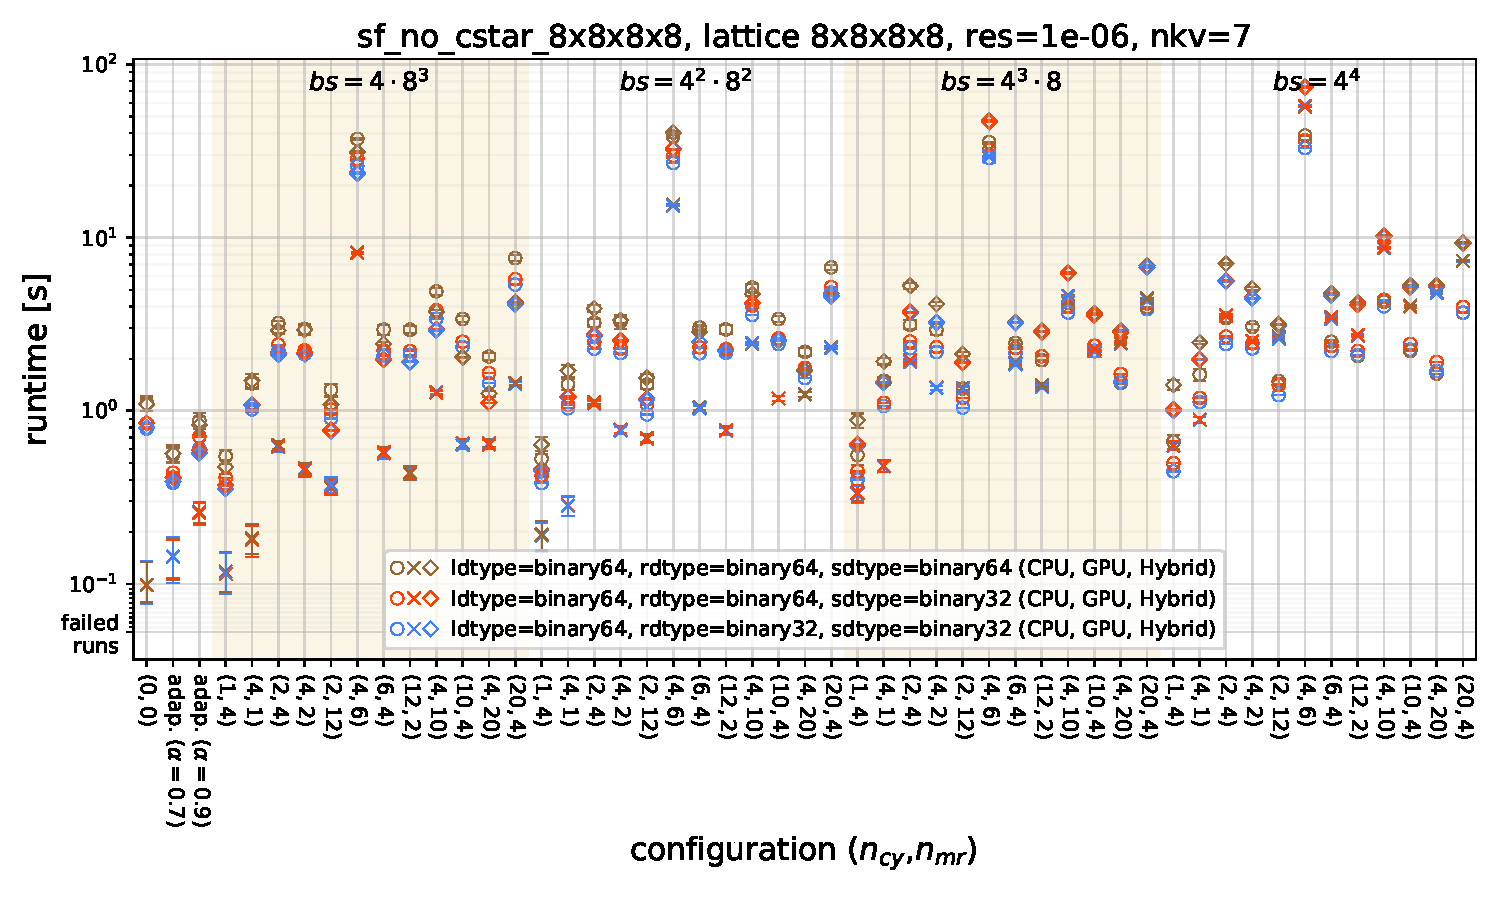
\includegraphics[width=1.0\textwidth]{plots/sap_gcr_sf_no_cstar_8x8x8x8_lattice_8x8x8x8_res=1e-06_nkv=7}
    \caption{Time measurements for the \code{SAP\_GCR} kernel on different matrices and configurations. The measurements were conducted on an AMD EPYC 7742 CPU @ 2.25GHz with 512 GB memory and an NVIDIA A100 (via SXM4) GPU with 40 GB memory.}
    \label{fig:sap_gcr0}
    \label{fig:sap_gcr_start}
    \label{fig:sap_gcr_sf_8x8x8x8}
\end{figure}

\begin{figure}[h]
    \centering
    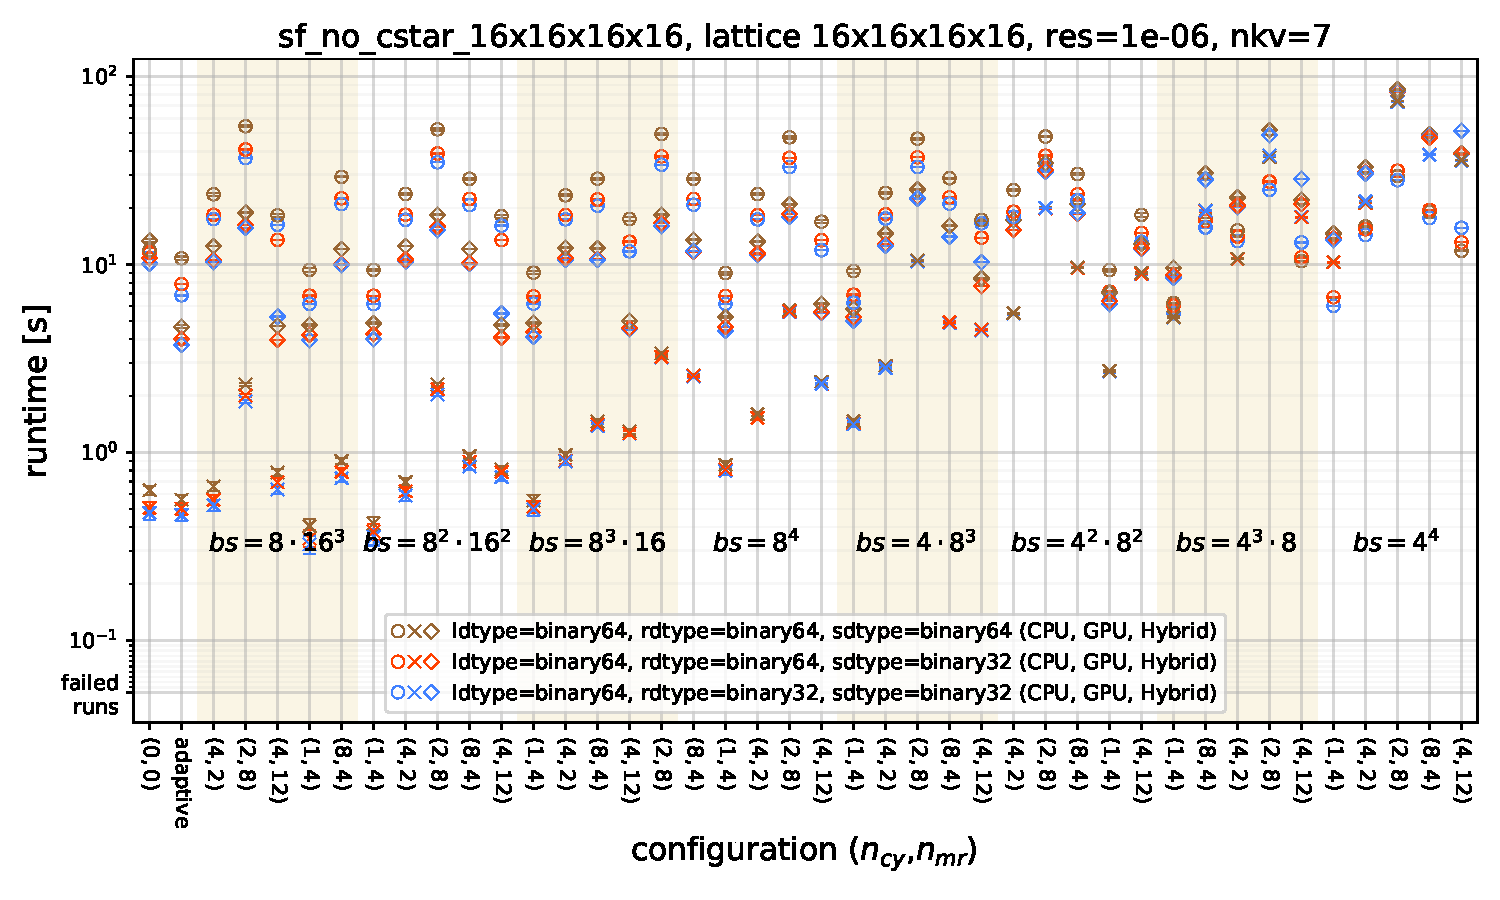
\includegraphics[width=1.0\textwidth]{plots/sap_gcr_sf_no_cstar_16x16x16x16_lattice_16x16x16x16_res=1e-06_nkv=7}
    \caption{Time measurements for the \code{SAP\_GCR} kernel on different matrices and configurations. The measurements were conducted on an AMD EPYC 7742 CPU @ 2.25GHz with 512 GB memory and an NVIDIA A100 (via SXM4) GPU with 40 GB memory.}
    \label{fig:sap_gcr3}
    \label{fig:sap_gcr_sf_16x16x16x16}
\end{figure}

\begin{figure}[h]
    \centering
    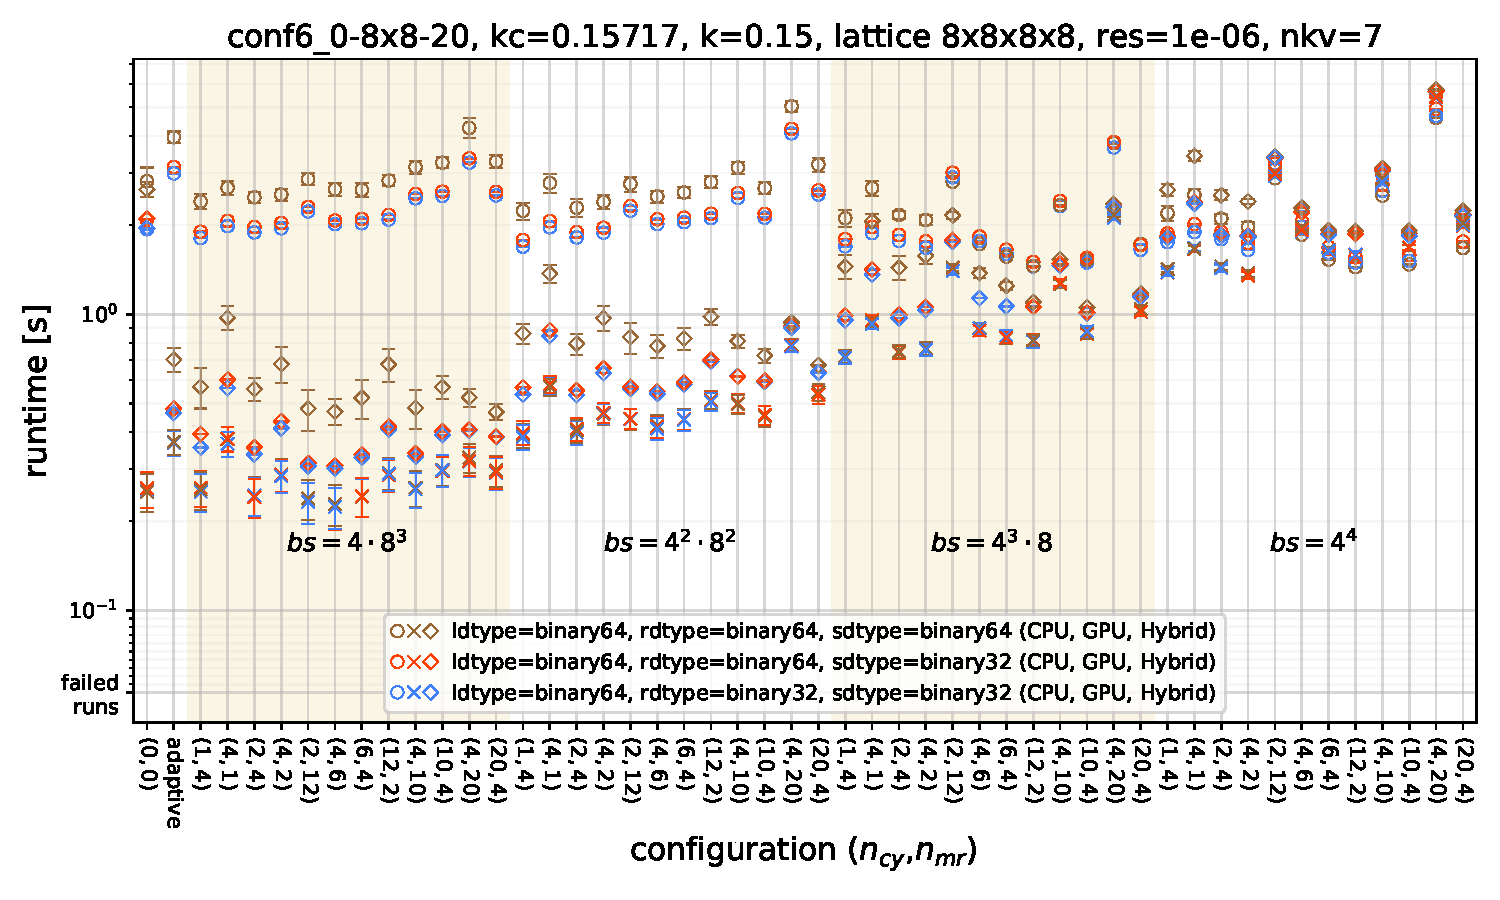
\includegraphics[width=1.0\textwidth]{plots/sap_gcr_conf6_0-8x8-20_kc=0.15717_k=0.15_lattice_8x8x8x8_res=1e-06_nkv=7}
    \caption{Time measurements for the \code{SAP\_GCR} kernel on different matrices and configurations. The measurements were conducted on an AMD EPYC 7742 CPU @ 2.25GHz with 512 GB memory and an NVIDIA A100 (via SXM4) GPU with 40 GB memory.}
    \label{fig:sap_gcr2}
    \label{fig:sap_gcr_conf6_0-8x8-20_0.15}
\end{figure}

\begin{figure}[h]
    \centering
    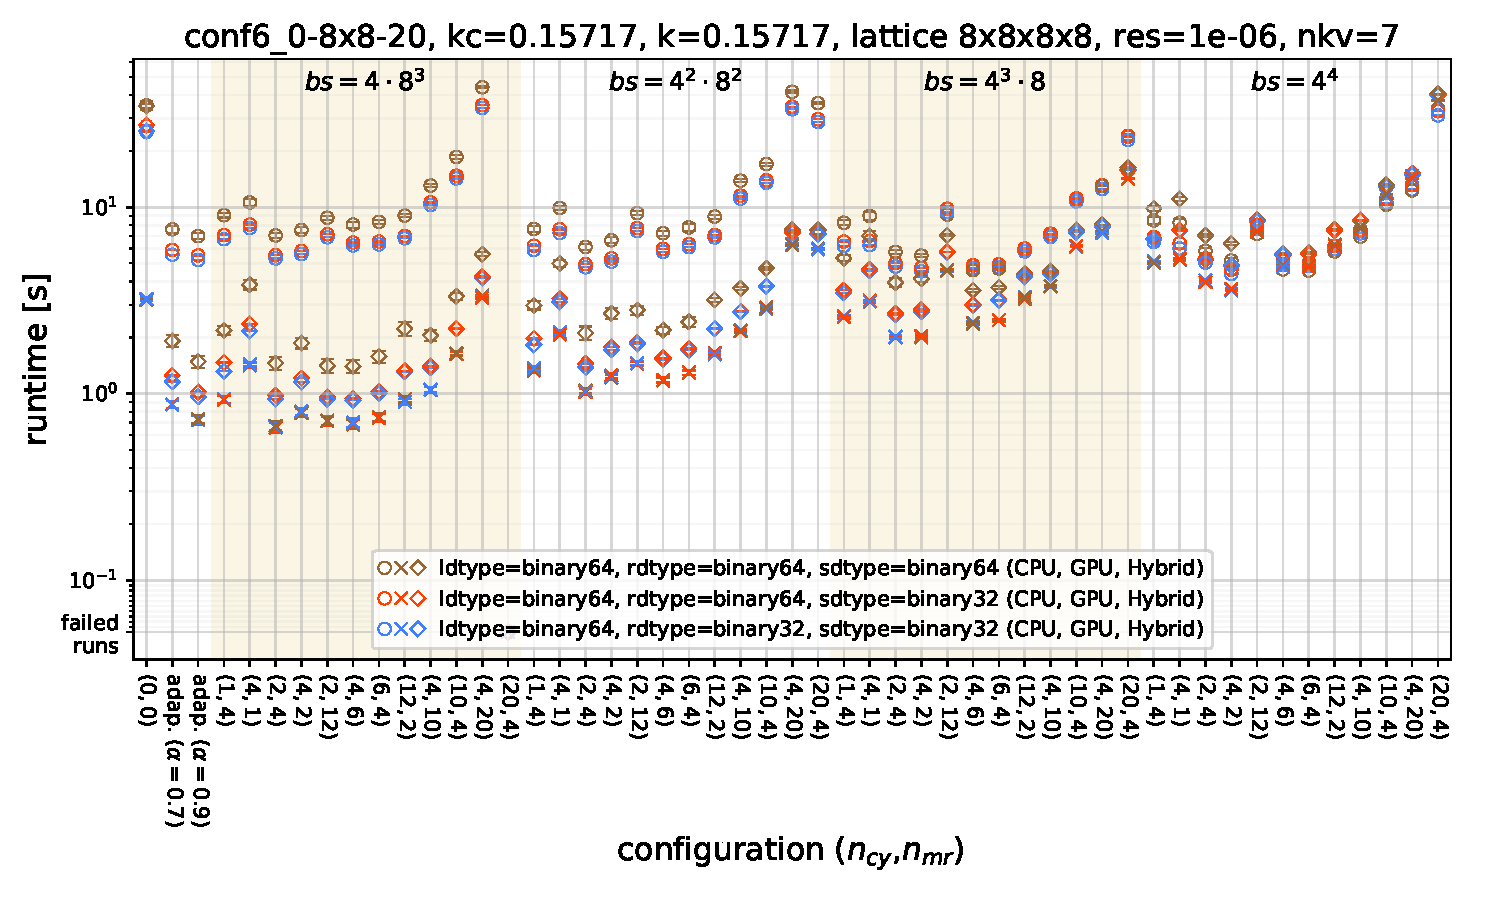
\includegraphics[width=1.0\textwidth]{plots/sap_gcr_conf6_0-8x8-20_kc=0.15717_k=0.15717_lattice_8x8x8x8_res=1e-06_nkv=7}
    \caption{Time measurements for the \code{SAP\_GCR} kernel on different matrices and configurations. The measurements were conducted on an AMD EPYC 7742 CPU @ 2.25GHz with 512 GB memory and an NVIDIA A100 (via SXM4) GPU with 40 GB memory.}
    \label{fig:sap_gcr1}
    \label{fig:sap_gcr_conf6_0-8x8-20_0.15717}
\end{figure}

\begin{figure}[h]
    \centering
    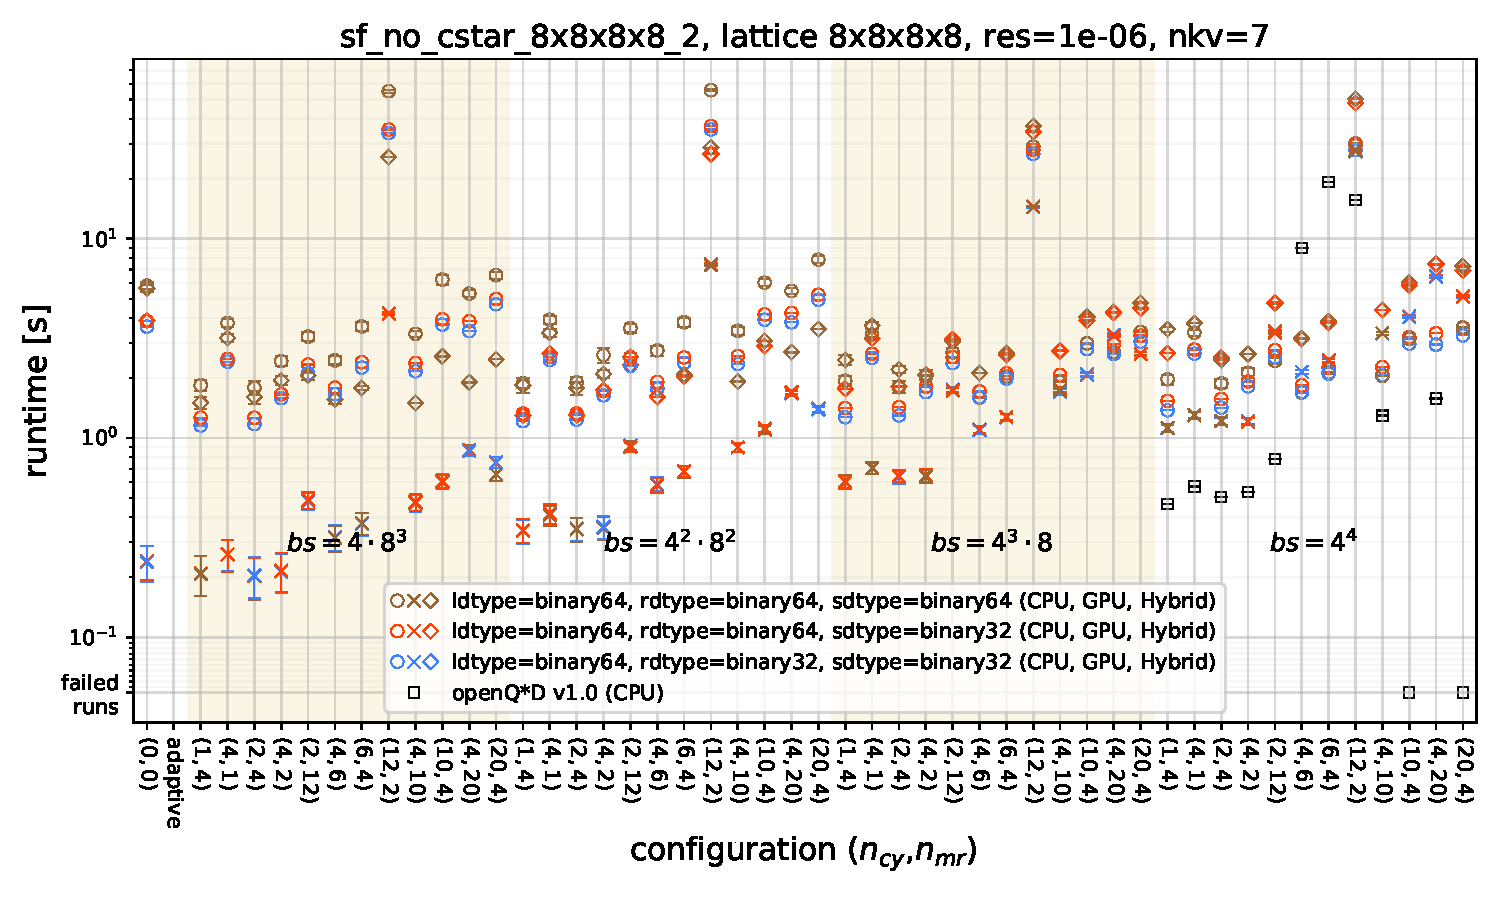
\includegraphics[width=1.0\textwidth]{plots/sap_gcr_sf_no_cstar_8x8x8x8_2_lattice_8x8x8x8_res=1e-06_nkv=7}
    \caption{Time measurements for the \code{SAP\_GCR} kernel on different matrices and configurations. The measurements were conducted on an Intel(R) 6130 @ 2.10GHz with 1.5 TB memory and an NVIDIA V100 (via PCIe) GPU with 16 GB memory.}
    \label{fig:sap_gcr4}
    \label{fig:sap_gcr_end}
    \label{fig:sap_gcr_sf_8x8x8x8_2}
\end{figure}

\subsubsection{Discussion of figures \ref{fig:sap_gcr_start} - \ref{fig:sap_gcr_end}}

A clear trend visible in the entire plot series is that the pure-GPU variants are most efficient when the block size is large (the number of blocks is small). The pure-CPU variants behave differently -- the block size has less influence on the run-time. In general, the pure-GPU variants are faster than the pure-CPU ones. This is because they take advantage of concurrency. The hybrid-variants are as expected in-between them, behaving similarly to the pure-GPU ones.

As a further general observation, the power of the \acrshort{sapgcr} solver is only fully unfolded if the condition number of the operator is large; figures \ref{fig:sap_gcr_sf_8x8x8x8}, \ref{fig:sap_gcr_sf_16x16x16x16} and \ref{fig:sap_gcr_sf_8x8x8x8_2} show no significant performance improvement of the SAP-preconditioning compared to a pure GCR solver without preconditioning\footnote{The runs with configuration $(n_{cy}, n_{mr}) = (0,0)$}, whereas the runs in figures \ref{fig:sap_gcr_conf6_0-8x8-20_0.15} and \ref{fig:sap_gcr_conf6_0-8x8-20_0.15717} do.

An analysis of the different data types shows that the general trend is the lower the involved data types are in bit-length, the faster the solution is obtained, which makes sense in memory-bound problems. The setups with \gls{binary32} in reduction variables (\code{rdtype}) and as "small" data type (\code{sdtype}) appear to be the most efficient. However, of the given data type setups one should choose the one where the data type of reduction variables (\code{rdtype}) is set to \gls{binary64} to prevent over- or underflows. This was already discussed in section \ref{sec:simulating_cgne} for the \acrshort{cgne}-solver.

\textbf{Figure \ref{fig:sap_gcr_sf_8x8x8x8}}: Looking at the first plot, figure \ref{fig:sap_gcr_sf_8x8x8x8}, as expected the preconditioning gives no significant improvement; on the CPU only \num{4} setups were faster than the one without preconditioning, on the GPU even none of the preconditioning setups surpasses the trivial case. All the CPU cases that were faster than the trivial case had the same configuration $(n_{cy}, n_{mr}) = (1,4)$, but different block sizes. This shows that if the operator is well-conditioned, too much preconditioning worsens the performance. $(n_{cy}, n_{mr}) = (1,4)$ is the configuration with the least amount of preconditioning. The CPU run-time shows a strong dependence on the configuration; there are even certain configurations (for example $(n_{cy}, n_{mr}) = (4,6)$) that are more than \num{40} times slower than the non-preconditioning case. An unsuitable choice of configuration parameters can thus lead to a significant performance degradation. However, the plots show that performance of the algorithm is overly sensitive to the choice of these parameters. The adaptive variant should here come to the rescue.

\textbf{Figure \ref{fig:sap_gcr_sf_16x16x16x16}}: The operator in figure \ref{fig:sap_gcr_sf_16x16x16x16} acting on a $16^4$-lattice has a similar behaviour as the previous one, because it is well-conditioned as well. The same configurations give a speedup compared to the case without preconditioning, this time both the CPU and GPU variants improved. The claim that the pure-GPU variant slows down with smaller block sizes is even more visible in this plot, since there are \num{8} block sizes to work on. Looking at the behaviour within a certain constant block size, the algorithm seems to be unpredictable sensitive to changes in the configuration. As an example, block size $bs= 8^2 \cdot 16^2$, one would expect the run-time to either increase or decrease with respect to the amount of preconditioning. The results show a more complex dependence with an exceptional case at $(n_{cy}, n_{mr}) = (2,8)$. This exceptional case can be seen in all block sizes and on the CPU, GPU as well as in the hybrid case. Figure \ref{fig:sap_gcr_sf_8x8x8x8} features such an exceptional case as well at $(n_{cy}, n_{mr}) = (4,6)$. However, with both matrices any preconditioning makes the run-time worse, they might not be very representative.

\textbf{Figure \ref{fig:sap_gcr_conf6_0-8x8-20_0.15}}: We continue the discussion with the matrix \code{conf6\_0-8x8-2} where the condition number depends on how close the $k = 0.15$ parameter is at its critical value $k_c = 0.15717$. This is the regime where the preconditioning shows benefits. For the pure-CPU cases, we see no strong dependence on the amount of preconditioning, but on the block size. Small block sizes seem to be beneficial, while the pure-GPU variant prefers large block sizes. Similar to the above analysis, the good condition number again gives not much speedup gain, when comparing the preconditioned cases with the trivial case.

\textbf{Figure \ref{fig:sap_gcr_conf6_0-8x8-20_0.15717}}: Using the same matrix as above, but at the critical point $k=k_c$, we are in the regime where the \acrshort{sapgcr} algorithm shows its true potential; nearly all cases performed better than the trivial case without any preconditioning. The pure-GPU cases behave as usual -- large block sizes result in faster convergence. This time even the pure-CPU shows a dependence on the block size. Although, this dependence is weak, the CPU seems to perform slightly better on smaller block sizes (on contrary to the GPU). The hybrid cases -- as usual in-between -- are closer to the pure-GPU ones, because despite being hybrid most of the work is done on the GPU. The pattern within a certain block size is repeating and the best amount of preconditioning seems to be at $(n_{cy}, n_{mr}) = (4,6)$.

\textbf{Figure \ref{fig:sap_gcr_sf_8x8x8x8_2}}: Finally, the second matrix from openQ*D \code{sf\_no\_cstar\_8x8x8x8\_2} shows similar patterns as the first matrix with the same configuration. The measurement was repeated in order to check whether there is a visible pattern common to both matrices. No such pattern were observed. It is noticeable that there is an exceptional configuration that took disproportionally longer than the others at $(n_{cy}, n_{mr}) = (12,2)$. More importantly it is not the same configuration as in figure \ref{fig:sap_gcr_sf_8x8x8x8}, making it hard to determine the best set of parameters beforehand and at the same time maintaining a perfect amount of preconditioning for all invocations of the solver throughout a long simulation.

%The discussion is just a more extreme version of the previous paragraph. Within all block sizes, one can see the same pattern repeating. It seems that the configurations involving substantial amounts of preconditioning (large \code{ncy}, \code{nmr}) perform worse.

\subsubsection{Conclusion}

In general, two different patterns can be observed in the above plot series. Either the matrix is bad conditioned, and one can see that most of the preconditioned runs perform better than no preconditioning. Or the matrix is good conditioned, and the preconditioned cases perform worse. In both cases the pattern within a block size repeats in other blocks sizes but shifted. We see two types of patterns. For bad conditioned systems, the pattern shows that the ideal case is at some point in the middle. On the other hand, for well-conditioned system, the pattern seems random, but an increase of run-time with more preconditioning (higher values of $n_{cy}$ and $n_{mr}$) can be seen. Since the systems are already well conditioned, too much preconditioning can worsen the run-time.


Since the algorithm is applied to many different Dirac-operators among evolving \acrshort{hmc}-trajectories -- some well-conditioned, some ill-conditioned -- it can be hard or even impossible to choose a set of parameters suitable for all cases. Especially, it is unavoidable to accidentally make a choice that falls on a configuration with exceptional long convergence time for a certain Dirac-operator within the long running HMC-simulation. It is therefore advisable to have the possibility to change the parameters during an active run or a configuration that adapts. This motivates the following proposal.

\begin{proposal}{Adaptive choice of parameters in \acrshort{sapgcr}}{adaptive}

Since the choice of parameters in the \acrshort{sapgcr} kernel seems non-trivial, we propose an adaptive variant of this algorithm. The parameters $n_{cy}$, $n_{mr}$ were chosen automatically in every iteration anew, the block size was chosen to be the largest possible. The adaptive choice was done as follows. If -- after a Schwarz-cycle -- the norm of the residual is not lower than the residual norm before the cycle, then the preconditioning phase is exited. Thus, at least one Schwarz-cycle is performed. A similar, but slightly more complicated strategy is applied to determine the number of MR-steps. There are \num{3} exit conditions for the MR-solver:

\begin{enumerate}[label={\arabic*)}]
  \item If -- after at least \num{4} MR-steps -- the norm of the residual on the block is larger than $\alpha = 0.9$\footnote{Ironically, the choice for the value of $\alpha \in (0, 1]$ is again non-trivial. Small values cause less preconditioning while values close to \num{1} will end up in more or even the maximal number of MR-steps. But since we want to optimise for ill-conditioned systems and the penalty for well-conditioned systems is acceptable, it is advisable to choose $\alpha$ large, such as $\alpha = 0.9$} times the previous residual norm, the MR-solver exits, and the application continues processing the next block.
  \item If the norm of the blocked residual becomes larger than the previous residual norm, the solver exits immediately, even if only one MR-step is executed.
  \item If the norm of the blocked residual is smaller than the tolerance\footnote{This is the tolerance calculated in the GCR solver divided by the number of blocks, $tol = res*\norm{\eta}/n_b$, where \code{res} is the desired relative residual given as configuration option (see table \ref{tab:sap_gcr_settings}), $\eta = \vec{b}$ is the source vector and $n_b$ is the number of blocks.}, the algorithm exit immediately too.
\end{enumerate}

So, every block is treated differently in every cycle. A maximum of \num{20} Schwarz-cycles and \num{20} MR-steps on each block would be performed if the above exit conditions never kick in. The third exit condition above makes sure to not overshoot the mark if the algorithm performs a lot of Schwarz-cycles and MR-steps. Namely, if the problem is already solved while in the preconditioning phase. This can happen if the operator is very well-conditioned or in the very last GCR-step before converging to the desired relative residual. Therefore, the adaptive version tries to find the optimal configuration for every iteration of the \acrshort{gcr}-solver, for every Schwarz-cycle and for every block separately. By empirical observation of the results, the adaptive variant usually performs nearly maximal amounts of preconditioning in the first few GCR-steps, then rapidly decreases after some steps to much smaller amounts and finally saturate to the minimal amount that stays until convergence.

The results on how this adaptive variant competes with static configurations can be seen in figures \ref{fig:sap_gcr_start} - \ref{fig:sap_gcr_end}. The adaptive runs are indicated with configuration $\text{adap. }(\alpha=0.9)$ and $\text{adap. }(\alpha=0.7)$. Although the adaptive variant of the algorithm is not the fastest among all configurations, the plots show that it is certainly the most versatile one. It can be of benefit if the condition of the operator is not known beforehand and might even change drastically within a long running simulation.

A reference implementation was written directly in openQ*D and can be found in the GitLab repository ref. \cite{gitlab_adaptive}.

\end{proposal}

%TODO: what to do with the following?
%In openQ*D, every rank has its own local lattice to process. The solver algorithms are implemented in a parallel manner, such that the solver is called on all ranks simultaneously. The simulation problem was chosen to be such that the task of one rank was compared on one single core of the CPU and on one single GPU (with all its parallelizability). It is therefore not surprising that in most cases, the GPU solved the problem much faster than the CPU. Keeping this in mind, it is natural to associate a larger local lattice to the available GPUs in the system (maybe 4-8 times larger, depending on the available memory) and let them participate to the solution of the full problem just as they were additional ranks (compare proposal \ref{pp:gpu_implementation1}).

\section{Deflated SAP preconditioned GCR}

\label{sec:dfl_sap_gcr}

Small quark masses corresponding to real physics are believed to be the cause for the spontaneous breaking of chiral symmetry in lattice QCD \cite{banks1980}. Numerical lattice QCD has the problem that with large lattice volumes and small quark masses simulation techniques become inefficient in the \df{chiral regime} (where chiral symmetry is spontaneously broken), because the Dirac-operators gets increasingly ill-conditioned. Thus, the presence of low eigenvalues is a source of difficulty \cite{giusti2003}. According to the Bank-Casher relation, see \cite{banks1980}, this is because the number of eigenvalues of $D$ below a fixed value grows with $O(V)$, where $V$ is the total 4D lattice volume. On the other hand, the computational effort scales even worse with $O(V^2)$, \cite{luscher2007}. This behaviour goes under the name of \df{$V^2$-problem}.

A solving algorithm that has a flat scaling with respect to the quark masses can therefore lead to large speedups specially in the chiral regime. The topic of this section is the deflated SAP+GCR algorithm, \acrshort{dflsapgcr}\footnote{Deflation -- as described in the following section -- can be applied to any linear solving algorithm.}. By deflating the Dirac-operator, it is possible to separate eigenmodes with small eigenvalues from the bulk. Thus, the space needs to be split in low and high modes without actually calculating the modes, else the problem would be solved already.

\subsection{Deflation}

\label{sec:deflation}

\begin{theorem}[Deflation]

\label{thm:deflation}

Let $A$ be a linear, invertible operator acting on a vector space $\Lambda$, $\vec{b} \in \Lambda$ an arbitrary vector and $P_L$ a projector\footnote{$P_L$ does not have to be orthogonal or Hermitian.} acting on $\Lambda$. Furthermore, define the linear operator $P_R$ such that $P_L A = A P_R$\footnote{Such a linear operator $P_R$ always exists -- just set $P_R \coloneqq A^{-1} P_L A$, since $A$ is invertible.}. Consider 

\begin{align}
    \vec{x}^{\star} \coloneqq P_R \vec{x}^{\star}_1 + (1-P_R) \vec{x}^{\star}_2, \label{eq:def_projection}
\end{align}

with $\vec{x}^{\star}_1$ and $\vec{x}^{\star}_2$ being solutions to the "smaller" (projected) systems

\begin{align*}
    P_L A \vec{x}_1 &= P_L \vec{b}
    & &\text{and} &
    (1-P_L)A \vec{x}_2 &= (1-P_L)\vec{b},
\end{align*}

respectively. Then 

\begin{enumerate}[label={\arabic*)}]
  \item $P_R$ is a projector,
  \item $\vec{x}^{\star}$ is the unique solution to $A\vec{x} = \vec{b}$.
\end{enumerate}

\end{theorem}

\begin{proof}

Using that $P_L^2 = P_L$ is a projector and the defining relation $P_L A = A P_R$,

\begin{align*}
    P_R^2 &= (A^{-1} P_L A)^2 \\
    &= A^{-1} P_L^2 A \\
    &= A^{-1} P_L A \\
    &= P_R.
\end{align*}

By direct calculation,

\begin{align*}
    A \vec{x}^{\star} &= A P_R \vec{x}^{\star}_1 + A (1-P_R) \vec{x}^{\star}_2 \\
    &= P_L A \vec{x}^{\star}_1 + (1-P_L) A \vec{x}^{\star}_2 \\
    &= P_L \vec{b} + (1-P_L)\vec{b} \\
    &= \vec{b}.
\end{align*}

Since $A$ is invertible $\vec{x}^{\star}$ is unique, although $\vec{x}^{\star}_1$ and $\vec{x}^{\star}_2$ may not be unique, their projections are.

\end{proof}

\begin{remark}
If we find clever subspaces in which the projectors $P_L$ and $P_R$ project without involving $A^{-1}$, we can solve $A\vec{x} = \vec{b}$ by solving the two smaller systems of equations and then projecting the solutions using $P_R$.
\end{remark}

\begin{remark}
Notice that $P_L A$ as well as $(1-P_L)A$ are not invertible. There are infinitely many solutions $\vec{x}^{\star}_1$ and $\vec{x}^{\star}_2$\footnotemark. Nonetheless the solution vector $\vec{x}^{\star}$ is still unique after the projection in equation \eqref{eq:def_projection}, because $P_R$ removes all ambiguity from $\vec{x}^{\star}_1$ and $\vec{x}^{\star}_2$.
\end{remark}

\footnotetext{Let $P$ be a linear projector (not the identity-operator) and $A$ an invertible linear operator. The system of interest is $PA\vec{x} = P\vec{b}$. There exists at least one solution to this, namely the unique solution to $A\vec{x} = \vec{b}$. Since $PA$ is not invertible, the only two possibilities are either zero or infinite solutions to $PA\vec{x} = P\vec{b}$, but it can't be zero solutions.}

\begin{remark}
Comparing deflation to left preconditioning, the difference is that in deflation $P_L$ is a projector and $P_L A$ has condition number infinite (but finite effective condition number) while in case of preconditioning $P_L $ is invertible (a good approximation of $A^{-1}$) and the condition number of $P_L A$ is expected to be smaller than the one of $A$. 
\end{remark}

\begin{remark}
If $A$ is positive definite, $P_L A$ is positive semi-definite and has condition number infinite. Furthermore, $P_L A \vec{x} = P_L \vec{b}$ has infinite solutions. Fortunately, such a system can be solved as long as the right-hand side is consistent, meaning that there exists an $\vec{x}$ solving $A \vec{x} = \vec{b}$, \cite{kaasschieter1988}.
\end{remark}

Therefore, it makes sense to define the relevant quantity.

\begin{definition}[Condition number]

The \df{condition number} $\kappa$ and the \df{effective condition number} $\kappa_{eff}$ of a matrix $A$ are the ratios between the largest and the smallest eigenvalues

\begin{align*}
    \kappa(A) &\coloneqq \frac{\abs{\lambda_{max}(A)}}{\abs{\lambda_{min}(A)}},
    & &\text{and} &
    \kappa_{eff}(A) &\coloneqq \frac{\abs{\lambda_{max}(A)}}{\abs{\lambda_{pmin}(A)}},
\end{align*}

where

\begin{align*}
  \abs{\lambda_{max}(A)} &\coloneqq \max \abs{\sigma(A)}, \\
  \abs{\lambda_{min}(A)} &\coloneqq \min \abs{\sigma(A)}, \\
  \abs{\lambda_{pmin}(A)} &\coloneqq \min \{ \abs{\lambda} \, \bigm\lvert \, \lambda \in \sigma(A), \abs{\lambda} > 0 \}.
\end{align*}

\end{definition}

\begin{remark}
The condition number and the effective condition number are equal if the matrix $A$ is invertible.
\end{remark}

\begin{corollary}

\label{cor:deflation}

Let $A$, $\Lambda$ and $\vec{b}$ be as in theorem \ref{thm:deflation}. Furthermore let $\{ \vec{\omega}_i \}_{i=1}^N$ be an orthonormal basis of a linear subspace $\Omega \subset \Lambda$, called the \df{deflation subspace} and let the restriction of $A$ to $\Omega$, $\widetilde{A} \coloneqq \restr{A}{\Omega}$ called the \df{little operator}, be invertible. Define $P_L$ by its action on an arbitrary vector $\vec{x} \in \Lambda$ as

\begin{align*}
    P_L \vec{x} &\coloneqq \vec{x} - \sum_{i,j=1}^N A \vec{\omega}_i (\widetilde{A}^{-1})_{ij} \langle \vec{\omega}_j, \vec{x} \rangle
    %P_R \vec{y} &= \vec{y} - \sum_{i,j=1}^N \vec{\omega}_i (\widetilde{A}^{-1})_{ij} \langle \vec{\omega}_j, A \vec{y} \rangle,
\end{align*}

and let $\vec{x}^{\star}_1$ be one of the (infinite) solutions to the \df{deflated system} $\hat{A} \vec{x}_1 = P_L \vec{b}$, where $\hat{A} \coloneqq P_L A$ is called the \df{deflated operator}. Consider

\begin{align}
    \vec{x}^{\star} \coloneqq P_R \vec{x}^{\star}_1 + \sum_{i,j=1}^N \vec{\omega}_i (\widetilde{A}^{-1})_{ij} \langle \vec{\omega}_j, \vec{b} \rangle, \label{eq:defl_soln}
\end{align}

with $P_R$ satisfying $P_L A = A P_R$. Then $\vec{x}^{\star}$ is the unique solution to the linear system of equations $A \vec{x} = \vec{b}$.

\end{corollary}

\begin{proof}

Let's first show that $P_L^2 = P_L$ is a projector,

\begin{align*}
    P_L^2 \vec{x} &= P_L \left( \vec{x} - \sum_{i,j=1}^N A \vec{\omega}_i (\widetilde{A}^{-1})_{ij} \langle \vec{\omega}_j, \vec{x} \rangle \right) \\
    &= \vec{x} - 2 \sum_{i,j=1}^N A \vec{\omega}_i (\widetilde{A}^{-1})_{ij} \langle \vec{\omega}_j, \vec{x} \rangle + \sum_{i,j=1}^N A \vec{\omega}_i (\widetilde{A}^{-1})_{ij} \sum_{k,l=1}^N \langle \vec{\omega}_j, A \vec{\omega}_k \rangle (\widetilde{A}^{-1})_{kl} \langle \vec{\omega}_l, \vec{x} \rangle \\
    &= \vec{x} - 2 \sum_{i,j=1}^N A \vec{\omega}_i (\widetilde{A}^{-1})_{ij} \langle \vec{\omega}_j, \vec{x} \rangle + \sum_{i,j,l=1}^N A \vec{\omega}_i (\widetilde{A}^{-1})_{ij} \langle \vec{\omega}_l, \vec{x} \rangle \underbrace{\sum_{k=1}^N \underbrace{\langle \vec{\omega}_j, A \vec{\omega}_k \rangle}_{= \widetilde{A}_{jk}} (\widetilde{A}^{-1})_{kl} }_{= \delta_{jl}} \\
    &= \vec{x} - 2 \sum_{i,j=1}^N A \vec{\omega}_i (\widetilde{A}^{-1})_{ij} \langle \vec{\omega}_j, \vec{x} \rangle + \sum_{i,j=1}^N A \vec{\omega}_i (\widetilde{A}^{-1})_{ij} \langle \vec{\omega}_j, \vec{x} \rangle \\
    &= \vec{x} - \sum_{i,j=1}^N A \vec{\omega}_i (\widetilde{A}^{-1})_{ij} \langle \vec{\omega}_j, \vec{x} \rangle \\
    &= P_L \vec{x}.
\end{align*}

The second term in equation \eqref{eq:defl_soln} is equal to $(1-P_R)\vec{x}^{\star}_2$ where $\vec{x}^{\star}_2$ solves the projected system $(1-P_L)A \vec{x}_2 = (1-P_L) \vec{b}$:

\begin{align*}
    (1-P_R)\vec{x}^{\star}_2 &= A^{-1} (1-P_L) A \vec{x}^{\star}_2 \\
    &= A^{-1} (1-P_L) \vec{b} \\
    &= A^{-1} \sum_{i,j=1}^N A \vec{\omega}_i (\widetilde{A}^{-1})_{ij} \langle \vec{\omega}_j, \vec{b} \rangle \\
    &= \sum_{i,j=1}^N \vec{\omega}_i (\widetilde{A}^{-1})_{ij} \langle \vec{\omega}_j, \vec{b} \rangle,
\end{align*}

which corresponds to the second term of $\vec{x}^{\star}$ in equation \eqref{eq:defl_soln}, therefore $\vec{x}^{\star} \coloneqq P_R \vec{x}^{\star}_1 + (1-P_R) \vec{x}^{\star}_2$. By application of theorem \ref{thm:deflation}, $\vec{x}^{\star}$ is the unique solution to $A\vec{x} = \vec{b}$.

\end{proof}

\begin{remark}
From $P_L$ in corollary \ref{cor:deflation}, the action of $P_R$ on an arbitrary vector $\vec{x}$ can be determined using the defining relation of $P_R$ as

\begin{align*}
    P_R\vec{x} &= A^{-1} P_L A \vec{x} \\ 
    &= \vec{x} - \sum_{i,j=1}^N \vec{\omega}_i (\widetilde{A}^{-1})_{ij} \langle \vec{\omega}_j, A \vec{x} \rangle.
\end{align*}
\end{remark}

\begin{remark}
An application of $P_L$ to an arbitrary vector $\vec{x}$ involves solving the \df{little system} $\widetilde{A} \vec{\beta} = \vec{\alpha}$ on $\Omega$ for a given $\vec{\alpha} \in \Omega$. To see this, let's look at the $k$-th component of $P_L \vec{x}$,

\begin{align*}
    (P_L\vec{x})_k &\coloneqq x_k - \sum_{i,j=1}^N (A\vec{\omega}_i)_k (\widetilde{A}^{-1})_{ij} \langle \vec{\omega}_j, \vec{x} \rangle.
\end{align*}

Define the vector

\begin{align*}
    \vec{\alpha}_{\vec{x}} &\coloneqq
    \begin{pmatrix}
        \langle \vec{\omega}_1, \vec{x} \rangle \\
        \langle \vec{\omega}_2, \vec{x} \rangle \\
        \vdots \\
        \langle \vec{\omega}_N, \vec{x} \rangle
    \end{pmatrix} = \begin{pmatrix}
        (\vec{\omega}_1)_1 & \hdots & (\vec{\omega}_1)_N \\
        (\vec{\omega}_2)_1 & \hdots & (\vec{\omega}_2)_N \\
        \vdots & \ddots & \vdots \\
        (\vec{\omega}_N)_1 & \hdots & (\vec{\omega}_N)_N
    \end{pmatrix} \begin{pmatrix}
        x_1 \\
        x_2 \\
        \vdots \\
        x_N
    \end{pmatrix}.
\end{align*}

Then,

\begin{align*}
    (P_L\vec{x})_k &= x_k - \sum_{i=1}^N (A\vec{\omega}_i)_k ( \textcolor{cyellow}{\widetilde{A}^{-1} \vec{\alpha}_{\vec{x}}} )_i \\
    &= x_k - \sum_{i=1}^N (A\vec{\omega}_i)_k \textcolor{cyellow}{\vec{\beta}}_i.
\end{align*}

By similar analysis, an application of $P_R$ has the same cost with one additional application of $A$. For an efficient implementation of $P_L$ and $P_R$, the $2N$ vectors $\{A\vec{\omega}_i\}_{i=1}^N$ and $\{\vec{\omega}_i\}_{i=1}^N$ have to be kept in memory.

\end{remark}

\begin{remark}

% TODO: work through this again -> local coherence

We assume that the condition number of $A$ is high and the \df{spectrum} of $A$, $\sigma(A)$, is separable in a way such that

\begin{align}
    \sigma(A) &= \sigma_l(A) \cup \sigma_h(A)
    & &\text{with} &
    \max\limits_{\lambda \in \sigma_l(A)} \abs{\lambda} &\ll \min\limits_{\lambda \in \sigma_h(A)} \abs{\lambda}. \label{eq:separable}
\end{align}

The subscripts stand for "low" and "high", corresponding to the low and high modes of the operator $A$. The property in equation \eqref{eq:separable} states that the bulk of the low eigenvalues are somewhat clustered\footnote{The high eigenmodes may not be clustered, but still separated from the low ones.}. Consider the linear sub-spaces $\Omega_l, \Omega_h \subset \Lambda$ such that the low and high eigenvectors corresponding to the low and high eigenvalues of $A$ are contained in $\Omega_l$ and $\Omega_h$, respectively. Then the condition number of $A$ restricted to the low modes is much smaller than the condition number of $A$. Therefore, if we are able to find an orthonormal basis $\{\vec{\omega}_i\}_{i=0}^N$ of the subspace $\Omega_l$ containing the bulk of the low eigenmodes of $A$, we can apply deflation from corollary \ref{cor:deflation} to solve the little equation that has a significantly smaller condition number than $A$. Then find one of the infinite solutions to the deflated system and construct a solution of the full system.

\end{remark}

\begin{lemma}
\label{lem:condition_number}

Let $A$, $\{\vec{\omega}_i\}_{i=1}^N \in \Omega$, $P_L$, $P_R$ be as in corollary \ref{cor:deflation} and assume that the spectrum of $A$ is separable, equation \eqref{eq:separable}. Define the deflation subspace to be the subspace corresponding to the low eigenmodes, $\Omega \coloneqq \Omega_l$. Then $\kappa_{eff}(\hat{A}) \ll \kappa(A)$ and $\kappa(\tilde{A}) \ll \kappa(A)$.
\end{lemma}

\begin{proof}

Let's define the orthogonal projector $P^{\perp}$ to $\Omega^{\perp}$, the orthogonal complement of the deflation subspace $\Omega$,

\begin{align*}
    P^{\perp} \vec{x} \coloneqq \vec{x} - \sum_{i=1}^N \langle \vec{\omega}_i, \vec{x} \rangle \vec{\omega}_i.
\end{align*}

The deflated operator $\hat{A} \coloneqq P_L A$ acts on the orthogonal complement,

\begin{align*}
    \hat{A} P^{\perp} \vec{x} &= P_L A P^{\perp} \vec{x} \\
    &= P_L A \vec{x} - \sum_{k=1}^N P_L A \vec{\omega}_k \langle \vec{\omega}_k, \vec{x} \rangle \\
    &= A \vec{x} - \sum_{i,j=1}^N A \vec{\omega}_i (\widetilde{A}^{-1})_{ij} \langle \vec{\omega}_j, A \vec{x} \rangle - \sum_{k=1}^N A \vec{\omega}_k \langle \vec{\omega}_k, \vec{x} \rangle + \sum_{i,k=1}^N A \vec{\omega}_i \underbrace{ \sum_{j=1}^N (\widetilde{A}^{-1})_{ij} \underbrace{\langle \vec{\omega}_j, A \vec{\omega}_k \rangle}_{=\widetilde{A}_{jk}} }_{\delta_{ik}} \langle \vec{\omega}_k, \vec{x} \rangle \\
    &= A \vec{x} - \sum_{i,j=1}^N A \vec{\omega}_i (\widetilde{A}^{-1})_{ij} \langle \vec{\omega}_j, A \vec{x} \rangle - \sum_{k=1}^N A \vec{\omega}_k \langle \vec{\omega}_k, \vec{x} \rangle + \sum_{k=1}^N A \vec{\omega}_k \langle \vec{\omega}_k, \vec{x} \rangle \\
    &= A \vec{x} - \sum_{i,j=1}^N A \vec{\omega}_i (\widetilde{A}^{-1})_{ij} \langle \vec{\omega}_j, A \vec{x} \rangle \\
    &= P_L A \vec{x} \\
    &= \hat{A} \vec{x}.
\end{align*}

\begin{comment}
Futher, define the \df{minimal and maximal eigenvalue} of an operator $A$,

\begin{align*}
    \lambda_{max}(A) &\coloneqq \max\limits_{\lambda \in \sigma(A)} \abs{\lambda}, \\
    \lambda_{min}(A) &\coloneqq \min\limits_{\lambda \in \sigma(A)} \abs{\lambda}, \\
    \lambda_{pmin}(A) &\coloneqq \min\limits_{\lambda \in \sigma(A), \abs{\lambda} > 0} \abs{\lambda}.
\end{align*}
\end{comment}

This now means, that the low eigenmodes are projected to zero, and do not participate to the effective condition number of $\hat{A}$, which can now be upper bounded,

\begin{align*}
    \kappa_{eff}({\hat{A}}) = \frac{\abs{\lambda_{max}(\hat{A})}}{\abs{\lambda_{pmin}(\hat{A})}} = \frac{\abs{\lambda_{max}(A)}}{\abs{\lambda_{pmin}(\hat{A})}} \ll \frac{\abs{\lambda_{max}(A)}}{\abs{\lambda_{min}(A)}} = \kappa({A}),
\end{align*}

where property \eqref{eq:separable} was used in the second inequality. Similarly, for the condition number of the little operator $\kappa({\tilde{A}})$ where we have $\sigma(\tilde{A}) = \sigma(\restr{A}{\Omega}) = \sigma_l$ which directly implies $\kappa(\tilde{A}) \ll \kappa(A)$. 

\end{proof}

\begin{remark}
Lemma \ref{lem:condition_number} tells us that the deflated and the little system are significantly better conditioned than the full system and both are therefore solved in fewer iterations\footnote{Additionally, the little system is much smaller in size than the full system, but the sparsity will not stay -- it might even become dense. The precision up to which this system has to be solved in an application of the projector is usually a fraction of the desired precision of the full solution.}. This holds only if we can find the subspace corresponding to the low eigenmodes $\Omega_l$ and if the low eigenvalues of the matrix are somewhat isolated from the bulk of the eigenvalues. Equation \eqref{eq:separable} gives us a condition on $A$ for an efficient deflation.
\end{remark}

%TODO: evtl. weg damit lemma 9.4

\begin{lemma}

$P_L$ as defined in corollary \ref{cor:deflation} is a projection to the orthogonal complement of $\Omega$, i.e. $\langle \vec{\omega}_k, P_L \vec{x} \rangle = 0$.

\end{lemma}

\begin{proof}

Let $\vec{x}$ be an arbitrary vector, and $k \in \{1, \dots, N\}$, then

\begin{align*}
    \langle \vec{\omega}_k, P_L \vec{x} \rangle &= \langle \vec{\omega}_k, \vec{x} \rangle - \sum_{i,j=1}^N \langle \vec{\omega}_k, A \vec{\omega}_i \rangle (\widetilde{A}^{-1})_{ij} \langle \vec{\omega}_j, \vec{x} \rangle \\
    &= \langle \vec{\omega}_k, \vec{x} \rangle - \sum_{j=1}^N \langle \vec{\omega}_j, \vec{x} \rangle \sum_{i=1}^N \widetilde{A}_{ki} (\widetilde{A}^{-1})_{ij} \\
    &= \langle \vec{\omega}_k, \vec{x} \rangle - \sum_{j=1}^N \langle \vec{\omega}_j, \vec{x} \rangle \delta_{kj} \\
    &= 0.
\end{align*}

\end{proof}

\subsection{Choosing the deflation subspace}

\label{sec:dfl_subspace}

Besides isolated low eigenmodes, the Dirac-operator should feature another property for deflation to be efficient. The computational cost to find an approximation of the low-mode deflation subspace should not be too high. It turns out that if the low eigenmodes of the Dirac-operator possess a certain property, only a few low eigenmodes are needed to construct a good approximation of the subspace of low eigenmodes $\Omega_l$. If the subspace of low eigenmodes is only approximated, the method is called \df{inexact deflation}.

\begin{comment}
\begin{definition}[Local coherence]

\label{def:local_coherence}

Let $\varepsilon > 0$, $M,N \in \mathbb{N}$ with $M \ll N$ and $\Lambda$ be the full lattice. Let $B \coloneqq \{\vec{\beta}_i\}_{i=1}^N$ and $C \coloneqq \{\vec{\gamma}_j\}_{j=1}^M$ with $\vec{\beta}_i,\vec{\gamma}_j \in \Lambda$ be two sets of fields. Furthermore, define the projector $P_{\Gamma}$ to the subspace $\Gamma \coloneqq span(C)$ via its action onto an arbitrary vector $\vec{x} \in \Lambda$ as

\begin{align*}
    P_{\Gamma} \vec{x} \coloneqq \sum_{j=1}^M \langle \vec{\gamma}_j, \vec{x} \rangle \vec{\gamma}_j.
\end{align*}

The fields $B$ are \df{locally coherent} with the fields $C$ up to $\varepsilon$, if $\forall i \in \{1, \dots N\}$

\begin{align*}
    \norm{ (1-P_{\Gamma}) \vec{\beta}_i } \le \varepsilon.
\end{align*}

\end{definition}
\end{comment}

\begin{definition}[Local coherence] % 2nd approach to a definition of local coherence

\label{def:local_coherence}

Let $1 \gg \varepsilon > 0$ and $\{\Omega_i\}_{i=1}^{n_b}$ be a decomposition of the full lattice $\Lambda$ into $n_b$ blocks (for example as in section \ref{sec:ddecomp} figure \ref{fig:ddecomp}) and let $P_i$ be the projector to block $\Omega_i$. Furthermore define the \df{bootstrap set} $B = \{\vec{\beta_j}\}_{j=1}^M$ as a set of normalized fields satisfying $\norm{(1-P_{exact}) \vec{\beta}_j }^2 \le \varepsilon$, where $P_{exact}$ is a projector to $\Omega_{exact}$, a subspace of dimension $\dim{(\Omega_{exact})} = N \gg M = \dim{(\spn{B})}$. Define the projected fields $\vec{\omega}_{ij} \coloneqq P_i \vec{\beta}_j$, their subspace $\Omega_{inexact} = \spn{\{\vec{\omega_{ij}}\}_{i,j=1}^{n_b,M}}$ and the projector $P_{inexact}$ which projects to $\Omega_{inexact}$.

The fields in $\Omega_{exact}$ are called \df{locally coherent} up to deficits $\varepsilon$, if there exists a non-empty bootstrap set $B$, such that for all normalized $\vec{\psi} \in \Omega_{exact}$,

\begin{align*}
    \norm{(1-P_{inexact}) \vec{\psi}}^2 \le \varepsilon.
\end{align*}

The value of $\varepsilon$ is called the \df{deficit}.

\end{definition}

\begin{remark}
In the definition above the \df{bootstrap fields} $\vec{\beta_j} \in B$ are, to a good approximation, linear combinations of fields in $\Omega_{exact}$, because -- when projected to the complement of $\Omega_{exact}$ -- their norm nearly vanishes. For the same reason, the \df{bootstrap subspace} $\spn{B}$ is, to a good extent, a subspace of $\Omega_{exact}$.
\end{remark}

\begin{remark}
Definition \ref{def:local_coherence} can be interpreted such that the fields in $\Omega_{exact}$ can be well approximated by the (much fewer) bootstrap fields (by projecting them to the blocks), since the approximation error is smaller or equal to $\varepsilon$.
\end{remark}

\begin{remark}
Definition \ref{def:local_coherence} can also (very informally) be restated as $\Omega_{exact}$ is approximately the span of the projected bootstrap fields.
\end{remark}

\begin{remark}
It turns out that the low eigenmodes with subspace $\Omega_{exact} = \Omega_l$ of the Dirac-operator are locally coherent\footnote{This is not proven, but numerical experiments show a strong indication of local coherence, \cite{luscher2007}.}.
\end{remark}

It remains to describe how to obtain the $M$ bootstrap fields $\vec{\beta_j}$. Ideally, they should be low eigenmodes of the Dirac-operator or linear combinations thereof. Usually, one starts with randomly generated vectors and repeatedly applies the inverse power method (see theorem \ref{thm:inverse_power_method} in appendix \ref{sec:inverse_power_method}). The resulting vectors may not be exact eigenvectors, but the components associated to the complement of the low modes quickly decrease after some inverse iteration steps (see corollary \ref{cor:inverse_power_method} in appendix \ref{sec:inverse_power_method}). These vectors are then, up to some $\varepsilon > 0$, linear combinations of low eigenmodes and can thus be used as bootstrap fields to generate a subspace that approximates the low eigenmode subspace well. At this point the property of local coherence can be exploited and efficient deflation subspaces can be generated from these fields by projecting them onto some block decomposition.

To summarize the results, if the Dirac-operator has a spectrum that is separable in the sense of equation \eqref{eq:separable} and the low eigenmodes are locally coherent for a small $\varepsilon$, then inexact deflation can be applied to solve the ill-conditioned Dirac equation and the procedure is more efficient than without deflation, because the deflated system is better conditioned (lemma \ref{lem:condition_number}). Moreover, generating the inexact deflation subspaces can be done efficiently using only a few low eigenmodes.

\begin{comment}
The larger the condition number the worse the problem to solve with iterative methods. But now we have 2 systems with condition numbers of infinity! Why is this better than one system with condition number < infinity? the smaller systems restricted to the projections space have condition numbers lower than the full system, IF the deflation space was chosen "wisely".
\end{comment}

\begin{comment}

Assuming that we have a $N$-dimensional subspace $\Omega \subset \Lambda$ of the full lattice $\Lambda$ and $\Omega$ is spanned by the orthonormal set of fields $\phi_1, \dots, \phi_N$, we can define the projector $P^{\Omega}$ to that subspace

\begin{align*}
    P^{\Omega} \colon \Lambda &\longrightarrow \Omega \\
    \psi(x) &\longmapsto P^{\Omega} \psi(x) \coloneqq \sum_{i=1}^N \langle \phi_i, \psi \rangle \phi_i(x).
\end{align*}

Since the $\phi_i$ describe a basis of the \df{deflation subspace} $\Omega$, the action of the Dirac operator $D$ on this subspace is completely determined by the components of the \df{little Dirac operator} $A^{\Omega} \colon \Omega \to \Omega$,

\begin{align*}
    A^{\Omega}_{ij} = \langle \phi_i, D \phi_j \rangle
\end{align*}

If the deflation subspace $\Omega$ approximates the bulk of the low eigenmodes in the spectrum of the Dirac operator, then the condition number of $D(\mathbb{I} - P)$ is smaller than that of $D$. This will speed up the convergence of an iterative solver algorithm.

\end{comment}

\begin{comment}

deflation

D denotes the lattice Dirac operator at a value of the bare quark mass close to the critical mass (the inverse of D is put in quotes in this formula in order to make it clear that an approximation to the inverse is being applied). As a result the components of the fields along the high modes of the Dirac operator are suppressed and the fields will therefore have a strong overlap with the subspace spanned by the low modes of the operator. The local coherence of the latter then guarantees that the associated domain-decomposed deflation subspace is highly effective


local coherence: Loosely speaking, a set of quark fields is referred to as locally coherent if the fields are locally well approximated by a relatively small number of fields

relaxation method: (like SAP preconditioning)

"deflating QCD": treating the eigenmodes of the Dirac operator with small eigenvalues separately from the bulk of the quark modes (eigenvalues)

"V^2 problem": # eigenvalues below a fixed value (ex: 100MeV) grows O(V = full 4D lattice volume). calculating low quark modes (low eigenvalues) scales with O(V^2)

"little dirac operator": Dirac op restricted to deflation subspace

clever choice of deflation subspace --> numerical effort O(V)

deflated system:
P_L D chi(x) = P_L eta(X)
P = projector to deflation subspace
P_L = projector to the orthogonal complement of the deflation subspace.

only the deflated system has to be solved, full system follows from the inverse of the deflated Dirac operator (whose condition number is expected to be significantly smaller that the full system)

little dirac operator can also be preconditioned using eo-preconditioning if the number of blocks in every direction is even.

* The application of the projector (P, P_L, P_R?) consumes 1/4 or more of the computation time!
* computation of the little Dirac operator takes a lot as well?

* bringing A in blockdiagonal form an then solve the problem on the 2 smaller block matrices on the diagonal
* Iterating this method, end up in a upper triagonal matrix -> gauss elimination

\end{comment}

\subsection{Simulating \acrshort*{dflsapgcr}}

\label{sec:dfl_sap_gcr_results}

\subsubsection{Setup}

The \acrshort{dflsapgcr}-kernel was implemented in Python by extending the already existing implementation of \acrshort{sapgcr}. Only the preconditioning phase has changed. The deflated variant of the algorithm takes the same arguments as the regular one, see table \ref{tab:sap_gcr_settings}. In addition to these settings, the deflated algorithm requires configuration options for the deflation subspace and the settings concerning the solver for the little equation, see table \ref{tab:dfl_sap_gcr_settings}.

\begin{table}[H]
\centering
    \begin{tabular}{ |p{1.5cm}|p{6cm}|p{4.5cm}|  }
        \hline
        setting & meaning & comment \\
        \hline\hline
        \code{Ns}  & number of bootstrap fields & \\
        \hline
        \code{bs}  & size of the deflation blocks & not to be confused with the block size for SAP \\
        \hline
        \code{res}  & desired relative residual & for solving the little equation \\
        \hline
        \code{nmx}  & maximal number of GCR steps & for solving the little equation \\
        \hline
    \end{tabular}
    \caption{Additional settings for \code{DFL\_SAP\_GCR} and their meanings. The first two options concern the generation of the deflation subspace, while the last two options deal with the little equation.}
    \label{tab:dfl_sap_gcr_settings}
\end{table}

The following plot series shows the interplay between deflation and Schwarz-preconditioning in terms of run-time. Figures \ref{fig:dfl_sap_gcr_start} - \ref{fig:dfl_sap_gcr_end} contain the measurements. The relative residual for the full system was chosen to the $10^{-9}$, the block size for the Schwarz-preconditioning is $4^4$ and the number of Krylov vectors until a restart was chosen to be $n_{kv} = 7$. The entire algorithm was executed on the CPU. Hybrid or pure-GPU runs are expected to look very similar in shape, but shifted in run-time. The number of required GCR-steps will be equal to the pure-CPU case. The plots show the dimension of the deflation subspace in $x$-direction and the amount of Schwarz-preconditioning in terms of $(n_{cy},n_{mr})$ in $y$-direction. The colors denote the run-time and the numbers within the blocks show the absolute run-time in seconds needed to solve the system and the number of outer GCR-steps needed until convergence (the value of the \code{status} variable). The time needed for the generation of the deflation subspaces is not included in the measurements. For each time measurement, the average of \num{10} runs was taken. A vanishing dimension of the deflation subspace, $\dim \Omega = N_s n_b = 0$, indicates that no deflation is applied to the problem. All deflation subspaces were generated by starting with $N_s$ random vectors and $n_b$ blocks to project onto, followed by applying the procedure described in section \ref{sec:dfl_subspace}. The number of inverse iteration steps was chosen to be $n_{inv} = 5$, where for each inversion one step of a \acrshort*{sapgcr}-solver was applied with $(n_{cy}, n_{mr}) = (5,4)$.

\begin{figure}[h]
    \centering
    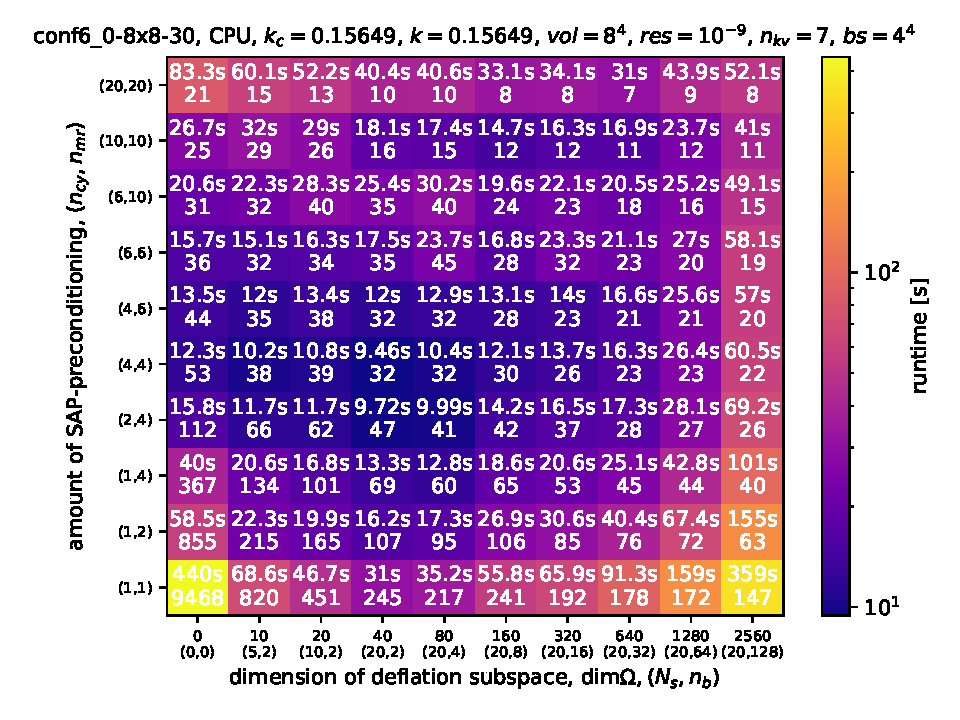
\includegraphics[width=1.0\textwidth]{plots/dfl_sap_gcr_conf6_0-8x8-30_8x8x8x8_k_0.15649}
    \caption{Time measurements for the \code{DFL\_SAP\_GCR} kernel on different matrices and configurations. The measurements were conducted on an Intel(R) 6130 @ 2.10GHz with 1.5 TB memory and an NVIDIA V100 (via PCIe) GPU with 16 GB memory.}
    \label{fig:dfl_sap_gcr0}
    \label{fig:dfl_sap_gcr_start}
    \label{fig:dfl_sap_gcr_conf6_0-8x8-30_8x8x8x8_k_0.15649}
\end{figure}

\begin{figure}[h]
    \centering
    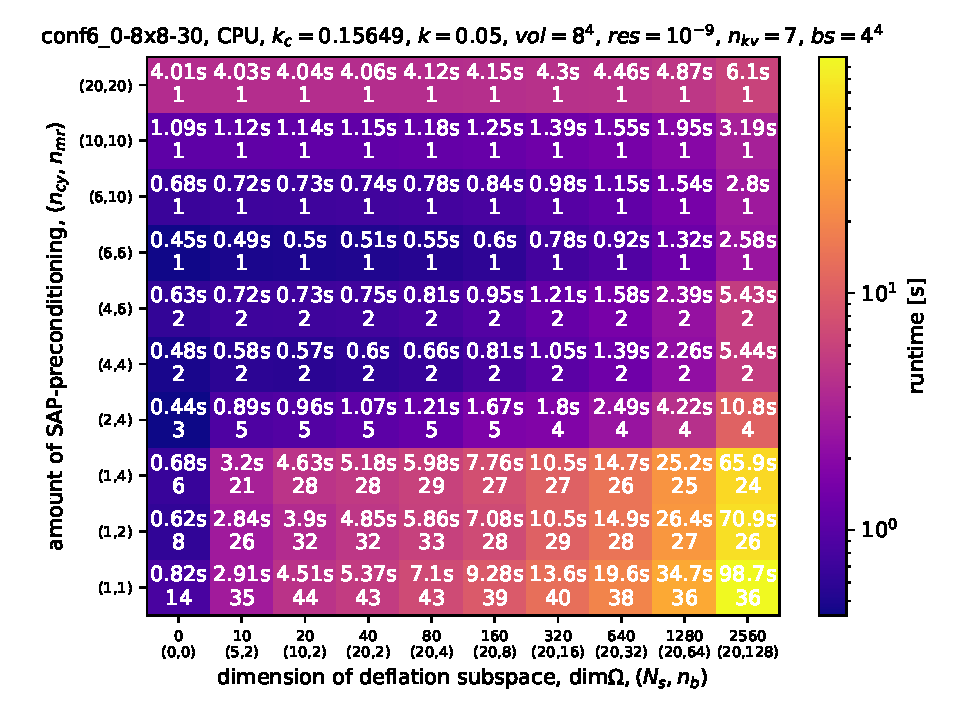
\includegraphics[width=1.0\textwidth]{plots/dfl_sap_gcr_conf6_0-8x8-30_8x8x8x8_k_0.05}
    \caption{Time measurements for the \code{DFL\_SAP\_GCR} kernel on different matrices and configurations. The measurements were conducted on an Intel(R) 6130 @ 2.10GHz with 1.5 TB memory and an NVIDIA V100 (via PCIe) GPU with 16 GB memory.}
    \label{fig:dfl_sap_gcr1}
    \label{fig:dfl_sap_gcr_conf6_0-8x8-30_8x8x8x8_k_0.05}
    \label{fig:dfl_sap_gcr_end}
\end{figure}

\subsubsection{Discussion of figures \ref{fig:dfl_sap_gcr_start} - \ref{fig:dfl_sap_gcr_end}}

The analysis was done on two Dirac-operators differing substancially in their condition number. The operator in figure \ref{fig:dfl_sap_gcr_conf6_0-8x8-30_8x8x8x8_k_0.15649} is bad-conditioned, while in figure \ref{fig:dfl_sap_gcr_conf6_0-8x8-30_8x8x8x8_k_0.05} the operator is close to the identity. It is expected that both plots show some similarity. Namely the number of GCR-steps needed should decrease when going from the lower left point upwards or to the right. There will be more preconditioning and deflation in the mentioned directions, leading to fewer needed GCR-steps. The configuration at the top right should thus have the least GCR-steps out of all configurations. However, this does not imply that it is the fastest, because each GCR-step involves heavy amounts of Schwarz-preconditioning, and the deflation subspace is the largest. Thus, the top right configuration is the one most intense in computational effort per GCR-step.

\textbf{Figure \ref{fig:dfl_sap_gcr_conf6_0-8x8-30_8x8x8x8_k_0.15649}}: Figure \ref{fig:dfl_sap_gcr_conf6_0-8x8-30_8x8x8x8_k_0.15649} is of special interest because the operator is in bad condition, thus well suited for delfation as well as Schwatrz-preconditioning. The pattern we observe has a bowl-shape, where the minimum is placed at some certain configuration. Configurations in the neighbourhood of the minimum perform similar. Starting from the minimum, the run-time increases in every direction. The \num{100} configurations considered seem to sample the configuration space quite well. The plot shows that there is a non-trivial interplay between preconditioning and deflation. Clearly, solving the little equation reduces the components of the full residue associated to the low eigenmodes. On the other hand, preconditioning consolidates the spectrum around the value \num{1}. This compactification affects the high modes more than the low modes, leading to a reduction of the high-mode components of the full residue. Therefore, the algorithm alternatives between treating the high and low mode components in the current solution vector.

\textbf{Figure \ref{fig:dfl_sap_gcr_conf6_0-8x8-30_8x8x8x8_k_0.05}}: In contrast to the previous operator, the matrix in figure \ref{fig:dfl_sap_gcr_conf6_0-8x8-30_8x8x8x8_k_0.05} is well-conditioned. The plot tells us that in this case low-mode deflation is a waste of resources. Theoretically, this can be understood, because a well-conditioned operator has no separable spectrum in the sense of equation \eqref{eq:separable}. Thus, the proofs in section \ref{sec:deflation} give us a reasoning why deflation is not efficient in this case. Applying the results from section \ref{sec:sap_gcr_results}, Schwarz-preconditioning should be kept within a tight limit for good conditioned systems. As stated previously, we expect the number of GCR-steps to decrease, when using larger deflation subspaces. On the contrary, when looking at the configuration $(n_{cy},n{mr}) = (1,1)$, we observe an \textit{increase} to the right instead. This suggests that too large deflation subspaces cause the solver to perform even worse, not only in run-time as it is with Schwarz-preconditioning, but also in the number of GCR-steps, finally leading to a regression. This specific operator has a clustering of all its eigenvalues around $1$. The exact low-mode eigenspace is still of the same size as for the operator in figure \ref{fig:dfl_sap_gcr_conf6_0-8x8-30_8x8x8x8_k_0.15649}, but the low-eigenvalues are not clearly separated anymore from the bulk of eigenvalues. A separation is thus harder to achieve, making the deflation subspace arbitrary and the deflation of the full system unprogressive and expensive. For deflation to be effective in such a case, one needs to determine the $N_s$ bootstrap vectors more precisely by using more inverse iteration steps, making the generation of deflation subspace computationally more expensive. Obviously, the better alternative would be to drop deflation entirely and minimize Schwarz-preconditioning for such a system.

\subsubsection{Conclusion}

The run-time seems to be convex in the dimension of the deflation subspace. This suggests that the true subspace of low eigenmodes lies approximately at the minimum of that convex curve. As a justification imagine that the subspace of low eigenmodes has dimension $d$, but the algorithm produced a subspace of dimension $d_1 \gg d$. This implies that the generated deflation subspace must contain high eigenmodes as well, making the little system increasingly ill-conditioned. This results in longer run-times, because the little equation has to be solved in every (outer) GCR-step. On the other hand, let's assume the algorithm generates a deflation subspace of dimension $d_2 \ll d$. Since only a few low eigenmodes can be split off, the deflated equation is still in bad condition (lemma \ref{lem:condition_number} does not apply). Although the little equation seems to be in good condition and small in its dimension, thus solved fast, it hardly contributes to the full solution. Again, resulting in longer run-times. Certainly, the perfect size for the deflation subspace is approximately the size of the subspace of the (exact) low eigenmodes. Of importance is that the bulk of the low eigenmodes is contained in it, such that the theorems of the previous section apply.

As mentioned before, the plots exhibit a bowl-shape, where the minimum gives the perfect balance between Schwarz-preconditioning and inexact low-mode deflation. The position of this minimum is certainly a property of the operator in consideration and depends on its condition number. If the number of low modes estimated with little computational effort, then together with the adaptive variant of the \acrshort*{sapgcr} algorithm one obtains a powerful and versatile solver.

Thinking about utilizing the GPU for the deflated solver, we see that the little equation should not be transferred to and solved on the GPU. Its dimensionality is a fraction of the full problem size, even for large lattices this is still small. Results in section \ref{sec:sap_gcr_results} show the GPU being efficient only on large sub-problems, while on small blocks it is clearly outperformed by the CPU. On the contrary, if the deflation is combined with Schwarz-preconditioning, the blocked problems can still be solved on the GPU efficiently and the conclusions of section \ref{sec:sap_gcr_results} apply.

\begin{comment}
\section{Multi-shift Conjugate Gradient}

TODO

\begin{proposal}{MSCG in mixed precision}{mscg_mp}

TODO: \acrlong{mscg} in mixed precision. Currently only in binary64.

\end{proposal}
\end{comment}

\section{Dirac operator}

\label{sec:dop}

\begin{comment}

The number of cycles in cg (or other solvers) do not scale with the lattice volume (times 12 which is the dimension of the matrix to solve), therefore the matrix becomes more sparse, the larger the lattice becomes. For very large lattice sizes D_dagger D starts to become proportional to the identity more and more, because the diagonal elements stay non-zero.

By ”Inversion” we mean inverting partially this matrix id est solving a set of equations of the type
Dψ=η (2.8)
where D and η are given and ψ is unknown. D is a 12N×12N complex matrix and η and ψ are 12N complex vectors. The solution is often called ”quark-propagator”. 

The gauge fields are SU(3) matrices. Inspecting their representations, they can be represented using 18, 12, 10 or 8 real numbers. The 8-representation involves 6 numbers between [-1,1] and 2 between [-pi,pi]. This is in all number ranges of all floating-point types! In QUDA, they use 16-bit (or 8-bit) signed integers and cudaReadModeNormalizedFloat to convert to a binary32 in the range [-1,1].

\end{comment}

The lattice Dirac-operator \eqref{eq:dwop} in openQ*D is implemented in terms of the various gauge-fields $U_{\mu}(n)$, only these are stored in memory\footnote{To be precise openQ*D also implements the Sheikholeslami-Wohlert-term \cite{sheikholeslami1985} which needs to store a set of fields as well and the boundary $O(a)$-improvement term that depends on two constants $c_F, c^{\prime}_F$, whose values depend on the chosen boundary conditions.}. In every HMC-trajectory the fields are updated, and the operator changes. In every Monte Carlo step the Dirac-operator has to be inverted for a given source vector to create the pseudofermion action, see equation \eqref{eq:pseudofermion_action}. The construction of correlation functions requires the inverse of the operator from a given source point to any other point on the lattice. This requires \num{12} rows or columns of $D^{-1}$, thus \num{12} inversions. Or simply calculating the fermion-propagator from one lattice point to another requires an inversion as well (see equation \eqref{eq:fermion_observables}). In summary, inverting the Dirac-operator takes about \num{90}\% of computation time in a lattice simulation. It is thus a fundamental kernel in every numerical lattice QFT calculation. Optimizing it increases the performance of \textit{any} solver.

\subsection{Dirac-operator with threads}

\label{sec:threads}

Modern processors today tend to have multiple cores. Two major programming models programmers are faced with are \acrshort{openmp} \cite{openmp45} and \acrshort{MPI} \cite{mpi}. Where MPI favours the scalability of large clusters with distributed memory, OpenMP favours speed of shared memory systems and the advantages of \acrfull{numa}. Comparing the two solutions gives motivation to look at OpenMP in more detail, especially considering OpenMP for intra-node traffic or traffic within a NUMA-domain. The goal is certainly a hybrid solution that keeps the scalability of MPI, but exploits NUMA-systems using OpenMP, since OpenMP seems to outperform MPI in most cases on a single node \cite{chan2011}.

\subsubsection{Terminology}

It makes sense to agree on terminology before analysing and discussing the results.

\begin{itemize}
    \item \df{Node}: Physical hardware device connected to the network of the supercomputer. Each node runs its instance of the operating system.
    \item \df{multicore CPU}: Hardware device that is attached to a socket. It consists of one or more physical cores on the same chip.
    \item \df{CPU, Processor, Physical core}: Hardware unit capable of independently performing basic arithmetic, logic, controlling, and (I/O) operations. A single physical core may correspond to one or more logical cores. Multiple physical cores may share L2 and L3 caches. Physical cores are associated to NUMA-nodes.
    \item \df{Logical core}: Logical cores are the abilities of a single physical core to execute two or more threads or processes concurrently. Logical cores associated to the same physical core share their caches.
    \item \df{Process, Rank}: As opposed to threads, processes or ranks do not share resources such as memory. Different instances of processes need to setup a communication channel to be able to communicate (using communication libraries such as MPI). 
    \item \df{Thread}: Sequence of programmed instructions. Multiple threads can execute concurrently and share resources such as memory. A process has always at least one thread (the master thread). A thread is spawned and joined by another thread. Communication among threads on the same node happens via shared memory.
    \item \df{NUMA-architecture}: A collection of NUMA-nodes linked by a point-to-point network. All cores, memory and devices are divided in NUMA-domains.
    \item \df{NUMA-node, NUMA-domain, NUMA-region}: A group of cores and/or memory and/or devices with \acrfull{uma}. Local memory is accessible to the other NUMA-nodes, but latency is generally higher than to their own local memory. Memory-bandwidth on the other hand can even be higher to other NUMA-nodes than to the one associated to. Not to be confused with the physical node.
\end{itemize}

\subsubsection{Setup}

The Dirac-operator in single-precision was implemented as a variant using threads according to the OpenMP standard in openQCD version 1.6 \cite{openqcd}. The performance of the operator was compared to the native implementation without threads. The runs were conducted on two different nodes having two vastly different processors, see tables \ref{tab:dop_omp_amd} and \ref{tab:dop_omp_intel}. On each node, \num{3} different lattice sizes were considered; $64^4$, $32^4$ and $16^4$. For each lattice size many configurations $(n_r,n_{th})$ were analysed, $n_r$ being the number of ranks and $n_{th}$ the number of threads. The configurations were chosen such that the machine was utilized half, fully or over-subscripted. Every configuration was executed \num{10} times, the average is quoted in the table. The exported OpenMP environment was:

\begin{lstlisting}[
    language=sh,
    numbers=none,
    label=lst:omp_env,
    caption={Environment variables for OpenMP.}
]
# each place corresponds to a core, threads are bound to cores
OMP_PLACES=cores
# block cyclic scheduling, where each thread gets floor(#iteration/#threads)
# contiguous iterations. In multiple parallel for-loops, all with the same
# scheduling policy and the same limits, the same threads get the same loop-slices
OMP_SCHEDULE=static
# assignment of threads to places goes successively through the available places
# as close to the master thread as possible
OMP_PROC_BIND=close
\end{lstlisting}

The runs were disposed using the mentioned environment variables and Slurms CPU-bind option to pin processes (and its threads) to NUMA-domains. Threads of the same rank were closely bound to cores within the same NUMA-regions whereas ranks were spread among NUMA-regions.

\subsubsection{Discussion}

\begin{table}
    \centering
    \begin{tabular}{ |p{1.5cm}||p{1cm}|p{1cm}|p{2cm}|p{2cm}|p{2cm}| }
        \hline
        & & & $64^4$ & $32^4$ & $16^4$ \\
        operator & $n_r$ & $n_{th}$ & time [s] & time [ms] & time [ms] \\
        \hline
        native & 256 & N/A & $1.06 \pm 0.02$ & $80.0 \pm 2.0$ & $9.53 \pm 0.33$ \\
        native & 128 & N/A & $1.06 \pm 0.01$ & $65.5 \pm 1.3$ & $6.63 \pm 0.73$ \\
        \hline
        omp & 128 & 1 & $1.12 \pm 0.06$ & $69.2 \pm 4.3$ & $6.32 \pm 0.13$ \\
        omp & 128 & 2 & $1.08 \pm 0.01$ & $71.8 \pm 6.0$ & $7.78 \pm 0.37$ \\
        omp & 128 & 4 & $1.09 \pm 0.01$ & $70.6 \pm 1.5$ & $9.90 \pm 2.68$ \\
        \hline
        omp & 64 & 1 & $1.54 \pm 0.08$ & $93.0 \pm 1.2$ & $7.14 \pm 0.17$ \\
        omp & 64 & 2 & $1.09 \pm 0.00$ & $66.6 \pm 3.9$ & $5.99 \pm 0.34$ \\
        omp & 64 & 4 & $1.07 \pm 0.01$ & $67.9 \pm 1.3$ & $8.39 \pm 0.40$ \\
        omp & 64 & 8 & $1.08 \pm 0.00$ & $70.7 \pm 1.7$ & $10.9 \pm 1.5$ \\
        \hline
        omp & 32 & 2 & $1.51 \pm 0.00$ & $94.1 \pm 0.3$ & $7.97 \pm 0.13$ \\
        omp & 32 & 4 & $1.09 \pm 0.00$ & $68.3 \pm 0.1$ & $6.87 \pm 0.24$ \\
        omp & 32 & 8 & $1.06 \pm 0.01$ & $72.6 \pm 0.8$ & $9.12 \pm 1.94$ \\
        omp & 32 & 16 & $1.09 \pm 0.00$ & $80.2 \pm 6.3$ & $11.7 \pm 0.7$ \\
        \hline
        omp & 16 & 4 & $1.60 \pm 0.01$ & $101 \pm 6$ & $8.83 \pm 0.10$ \\
        omp & 16 & 8 & $1.15 \pm 0.00$ & $79.9 \pm 0.8$ & $8.39 \pm 0.13$ \\
        omp & 16 & 16 & $1.13 \pm 0.01$ & $88.8 \pm 1.7$ & $10.9 \pm 1.0$ \\
        omp & 16 & 32 & $1.14 \pm 0.01$ & $92.7 \pm 1.8$ & $14.3 \pm 0.5$ \\
        \hline
        omp & 8 & 8 & $1.88 \pm 0.00$ & $131 \pm 7$ & $11.6 \pm 0.4$ \\
        omp & 8 & 16 & $1.26 \pm 0.01$ & $102 \pm 3$ & $10.7 \pm 0.1$ \\
        omp & 8 & 32 & $1.23 \pm 0.01$ & $110 \pm 7$ & $13.5 \pm 0.8$ \\
        omp & 8 & 64 & $1.30 \pm 0.03$ & $111 \pm 1$ & $19.7 \pm 0.6$ \\
        \hline
        omp & 4 & 16 & $2.01 \pm 0.01$ & $150 \pm 0$ & $14.3 \pm 0.1$ \\
        omp & 4 & 32 & $1.38 \pm 0.00$ & $124 \pm 1$ & $14.8 \pm 0.4$ \\
        omp & 4 & 64 & $1.36 \pm 0.02$ & $133 \pm 2$ & $19.4 \pm 0.4$ \\
        omp & 4 & 128 & $1.44 \pm 0.01$ & $134 \pm 4$ & $25.8 \pm 0.7$ \\
        \hline
        omp & 2 & 32 & $2.05 \pm 0.03$ & $169 \pm 6$ & $19.5 \pm 0.4$ \\
        omp & 2 & 64 & $1.50 \pm 0.05$ & $147 \pm 1$ & $19.6 \pm 0.6$ \\
        omp & 2 & 128 & $1.43 \pm 0.01$ & $167 \pm 3$ & $25.3 \pm 1.4$ \\
        omp & 2 & 256 & $1.49 \pm 0.03$ & $165 \pm 7$ & $34.0 \pm 1.3$ \\
        \hline
        omp & 1 & 64 & $2.17 \pm 0.00$ & $142 \pm 0$ & $12.5 \pm 0.2$ \\
        omp & 1 & 128 & $2.18 \pm 0.01$ & $144 \pm 3$ & $15.2 \pm 0.5$ \\
        omp & 1 & 256 & $2.19 \pm 0.01$ & $157 \pm 6$ & $17.4 \pm 0.8$ \\
        omp & 1 & 512 & $2.35 \pm 0.01$ & $171 \pm 3$ & $53.4 \pm 5.3$ \\
        \hline
    \end{tabular}
    \caption{\num{10} consecutive invocations of the single precision Dirac-operator \code{Dw()} on random fields in openQCD version 1.6. The table shows runs with different rank/thread configurations $(n_r, n_{th})$ on different lattice sizes. The lattice size refers to the total lattice size on the node. The node consisted of \num{2} NUMA-nodes, \num{2} sockets each with an AMD EPYC 7742 processor @ 2.25GHz with \num{64} physical cores per socket and \num{2} threads per core; in total \num{256} logical cores, with 512GB of memory. The cache sizes of one processor are L1 data: 2MB ($64 \times 32$KB), L1 instruction: 2MB ($64 \times 32$KB), L2: 32MB ($64 \times 512$KB), L3: 256MB ($16 \times 16$MB).}
    \label{tab:dop_omp_amd}
\end{table}

\textbf{Table \ref{tab:dop_omp_amd}}: In table \ref{tab:dop_omp_amd} the number of physical and logical cores was a power of \num{2}, therefore in both cases -- native and with threads -- all logical cores on the node could be utilized. In general, the best run-times were achieved with the native operator. The only exception for the $16^4$ lattice was the run with \num{64} ranks and \num{2} threads per rank. With that lattice size the entire gauge-field configuration fits into L2 cache of one processor (see table \ref{tab:lattice_sizes}), making consecutive runs very fast. Especially for the variant with threads, with twice as many threads the problem is not solved in half the time. This suggests that the overhead for dealing with threads is not negligible, and certainly needs improvement. It should be seen as a first working step towards hyper-threading. On the other hand, the native implementation lacks an ideal strong scaling, which can be seen by looking at the first two rows. Generally, the runs with only \num{128} ranks are faster than the runs using every of the \num{256} logical cores. This holds for all considered lattice sizes. Let's concentrate on the most interesting lattice size $64^4$. The variant with threads brings no benefit compared to the native one, but there are configurations that are comparable in run-time, namely the ones with $(n_r, n_{th})=(64,4)$ as well as $(32,8)$. Both make use of all logical cores on the node. Improving the thread implementation can therefore lead to a speedup increase (see conclusion). Generally, the less ranks, the worse the performance becomes. This can be explained by false sharing among the threads and ignorance concerning NUMA-effects when implementing the operator with threads.

\textbf{Table \ref{tab:dop_omp_intel}}: Table \ref{tab:dop_omp_intel} shows a vastly different picture: most notable for the analysis is the fact that the total number of physical and logical cores was \textit{not} a power of \num{2} on this node. This makes it difficult to utilize all resources using the native implementation. This fact is reflected by the results. The variant using threads has substantial performance increase compared to the best native pure-MPI implementation using \num{64} ranks. Especially the configurations with ranks and threads $(n_r, n_{th})=(16,7)$, $(8,14)$ and $(4,14)$ perform best. The reason for this lies in the non-trivial association of cores to NUMA-domains. The node has \num{4} NUMA-domains, where the logical cores are associated to NUMA-domains in a non-trival manner (see listing \ref{lst:lscpu}). \num{14} logical cores share an L3 cache. This explains why the mentioned configurations with \num{14} threads perform well. The jobs were disposed in a way that the \num{14} threads are bound to physical cores with the same L3 cache, thus cores in the same NUMA-domain. The job $(16,7)$ that performed best was disposed such that each of the \num{4} NUMA-domains contained a group of \num{4} consecutive ranks with \num{7} threads each. All \num{112} logical cores were utilized.

\begin{figure}
\begin{lstlisting}[
    language=C,
    numbers=none,
    label=lst:lscpu,
    caption={Output of \code{lscpu -e}. Notice the association of logical cores (first column) to NUMA-domains (second column). The fourth column denotes the physical core. Each NUMA-domain has \num{14} logical cores, where core \num{0} and \num{56} belong to physical core \num{0} sharing their L1 and L2 cache on NUMA-node \num{0}, logical cores \num{1} and \num{57} belong to physical core \num{1} on NUMA-node \num{0} sharing L1 and L2 cache and so on. The L3 cache is shared among logical cores \num{0}-\num{13} and \num{56}-\num{69}, \num{14}-\num{27} and \num{70}-\num{83}, and so on. One NUMA-domain has thus \num{14} physical and \num{28} logical cores.}
]
$ lscpu -e
CPU NODE SOCKET CORE L1d:L1i:L2:L3 ONLINE
0   0    0      0    0:0:0:0       yes
1   0    0      1    1:1:1:0       yes
2   0    0      2    2:2:2:0       yes
3   0    0      3    3:3:3:0       yes
4   0    0      4    4:4:4:0       yes
[...]
13  0    0      13   13:13:13:0    yes
14  1    1      14   14:14:14:1    yes
[...]
27  1    1      27   27:27:27:1    yes
28  2    2      28   28:28:28:2    yes
[...]
41  2    2      41   41:41:41:2    yes
42  3    3      42   42:42:42:3    yes
[...]
51  3    3      51   51:51:51:3    yes
52  3    3      52   52:52:52:3    yes
53  3    3      53   53:53:53:3    yes
54  3    3      54   54:54:54:3    yes
55  3    3      55   55:55:55:3    yes
56  0    0      0    0:0:0:0       yes
57  0    0      1    1:1:1:0       yes
58  0    0      2    2:2:2:0       yes
59  0    0      3    3:3:3:0       yes
60  0    0      4    4:4:4:0       yes
[...]
69  0    0      13   13:13:13:0    yes
70  1    1      14   14:14:14:1    yes
[...]
83  1    1      27   27:27:27:1    yes
84  2    2      28   28:28:28:2    yes
[...]
97  2    2      41   41:41:41:2    yes
98  3    3      42   42:42:42:3    yes
[...]
107 3    3      51   51:51:51:3    yes
108 3    3      52   52:52:52:3    yes
109 3    3      53   53:53:53:3    yes
110 3    3      54   54:54:54:3    yes
111 3    3      55   55:55:55:3    yes
\end{lstlisting}
\end{figure}

\begin{table}
    \centering
    \begin{tabular}{ |p{1.5cm}||p{1cm}|p{1cm}|p{2cm}|p{2cm}|p{2cm}| }
        \hline
        & & & $64^4$ & $32^4$ & $16^4$ \\
        operator & $n_r$ & $n_{th}$ & time [s] & time [ms] & time [ms] \\
        \hline
        native & 16 & N/A & $7.33 \pm 0.05$ & $450 \pm 3$ & $28.2 \pm 0.1$ \\
        native & 32 & N/A & $8.64 \pm 0.01$ & $538 \pm 2$ & $30.3 \pm 0.1$ \\
        native & 64 & N/A & $4.41 \pm 0.01$ & $280 \pm 0$ & $21.6 \pm 7.5$ \\
        \hline
        omp & 64 & 1 & $4.72 \pm 0.00$ & $298 \pm 0$ & $25.1 \pm 14.3$ \\
        omp & 64 & 2 & $4.74 \pm 0.01$ & $304 \pm 14$ & $24.3 \pm 6.2$ \\
        omp & 64 & 4 & $4.75 \pm 0.00$ & $300 \pm 0$ & $22.0 \pm 5.0$ \\
        omp & 64 & 8 & $4.77 \pm 0.00$ & $303 \pm 0$ & $24.9 \pm 4.0$ \\
        \hline
        omp & 32 & 1 & $9.33 \pm 0.03$ & $581 \pm 1$ & $33.7 \pm 0.1$ \\
        omp & 32 & 2 & $9.34 \pm 0.02$ & $583 \pm 1$ & $34.2 \pm 0.2$ \\
        omp & 32 & 4 & $9.36 \pm 0.01$ & $584 \pm 1$ & $35.4 \pm 0.1$ \\
        omp & 32 & 7 & $9.39 \pm 0.01$ & $590 \pm 0$ & $37.1 \pm 0.1$ \\
        \hline
        omp & 16 & 2 & $4.29 \pm 0.02$ & $269 \pm 2$ & $18.8 \pm 0.1$ \\
        omp & 16 & 4 & $4.62 \pm 0.02$ & $290 \pm 0$ & $18.3 \pm 0.1$ \\
        omp & 16 & 7 & $2.84 \pm 0.01$ & $190 \pm 1$ & $14.1 \pm 0.1$ \\
        omp & 16 & 14 & $4.04 \pm 0.00$ & $259 \pm 1$ & $20.8 \pm 0.1$ \\
        \hline
        omp & 8 & 4 & $4.55 \pm 0.04$ & $299 \pm 2$ & $21.9 \pm 0.0$ \\
        omp & 8 & 8 & $4.81 \pm 0.01$ & $318 \pm 0$ & $21.7 \pm 0.1$ \\
        omp & 8 & 14 & $3.08 \pm 0.01$ & $217 \pm 9$ & $17.7 \pm 0.5$ \\
        omp & 8 & 28 & $3.10 \pm 0.01$ & $217 \pm 0$ & $20.6 \pm 0.1$ \\
        \hline
        omp & 4 & 7 & $5.29 \pm 0.03$ & $353 \pm 1$ & $25.2 \pm 0.1$ \\
        omp & 4 & 14 & $3.09 \pm 0.02$ & $225 \pm 8$ & $18.0 \pm 0.1$ \\
        omp & 4 & 28 & $3.34 \pm 0.09$ & $238 \pm 1$ & $20.0 \pm 0.2$ \\
        omp & 4 & 56 & $3.32 \pm 0.01$ & $244 \pm 1$ & $25.3 \pm 0.1$ \\
        \hline
        omp & 2 & 28 & $4.87 \pm 0.01$ & $320 \pm 0$ & $21.8 \pm 0.1$ \\
        omp & 2 & 56 & $4.75 \pm 0.01$ & $326 \pm 1$ & $23.7 \pm 0.1$ \\
        omp & 2 & 112 & $4.73 \pm 0.01$ & $340 \pm 2$ & $33.7 \pm 1.2$ \\
        \hline
        omp & 1 & 56 & $5.50 \pm 0.01$ & $301 \pm 1$ & $17.3 \pm 0.1$ \\
        omp & 1 & 112 & $4.98 \pm 0.01$ & $314 \pm 1$ & $18.6 \pm 0.2$ \\
        omp & 1 & 224 & $5.13 \pm 0.01$ & $338 \pm 2$ & $36.3 \pm 0.2$ \\
        \hline
    \end{tabular}
    \caption{\num{10} consecutive invocations of the single precision Dirac-operator \code{Dw()} on random fields in openQCD version 1.6. The table shows runs with different rank/thread configurations $(n_r, n_{th})$ on different lattice sizes. The lattice size refers to the total lattice size on the node. The node consisted of \num{4} NUMA-nodes, \num{4} sockets each with an Intel(R) E7-4830 v4 @ 2.00GHz with \num{14} physical cores per socket and \num{2} threads per core; in total \num{112} logical cores, with 2TB of memory. The cache sizes of one processor are L1 data: 448KB ($14 \times 32$KB), L1 instruction: 448KB ($14 \times 32$KB), L2: 3.5MB ($14 \times 256$KB), L3: 35MB ($1 \times 35$MB).}
    \label{tab:dop_omp_intel}
\end{table}

\begin{table}
\centering
    \begin{tabular}{ |p{1cm}|p{2cm}|p{2cm}| }
        \hline
        lattice & gauge-field & quark-field \\
        \hline
        $16^4$ & 18MB & 6MB \\
        $32^4$ & 288MB & 96MB \\
        $64^4$ & 4608MB & 1536MB \\
        \hline
    \end{tabular}
    \caption{Sizes of the gauge- and quark-fields in terms of lattice sizes.}
    \label{tab:lattice_sizes}
\end{table}

\subsubsection{Conclusion}

The variant using threads is useful on machines where the number of logical or physical cores is not a power of \num{2}, or can somehow not be fully utilized by the pure-MPI implementation. Since in openQCD (and openQ*D) the number of ranks in one direction can only be $2,4,6,\dots$ and the lattice size in one direction can only be $4,6,8,\dots$, these numbers are limited for a given lattice size and a processor where the number of CPUs is not a power of \num{2}. Utilizing the entire node is not always possible\footnote{For example the node in table \ref{tab:dop_omp_intel}, where only a maximum of \num{64} from a total of \num{112} logical cores could be utilized.}. On the other hand, the operator with threads can utilize the entire node, because the number of threads per rank is arbitrary.

When implementing threads, it is important to write NUMA-aware code. In the above implementation there are certainly performance degradations due to NUMA-effects and false sharing. It was tried to obey the first-touch policy as often as possible, by initializing the involved arrays with a parallel for-loop, just as they are accessed later in the main for-loop\footnote{See line 1295ff in \code{modules/dirac/Dw.c} in \cite{openqcd_threads}} within the Dirac-operator. However, a certain amount of false sharing was not preventable without significantly changing the original code.

Another peculiarity of the above implementation was that in \code{deo()} the \num{8} directions of the gauge-fields had to be separately locked in every lattice point, because in these code segments the output vector was written leading to race conditions among threads without locking. The initialization and de-initialization of the \code{VOLUME/2} locks involve a non-negligible overhead in every call of the Dirac-operator. The overhead can be estimated by comparing the results of $(128, N/A)$ and $(128, 1)$ in table \ref{tab:dop_omp_amd} or $(64, N/A)$ and $(64, 1)$ in table \ref{tab:dop_omp_intel}.

\begin{proposal}{The Dirac-operator with threads}{dop_threads}

The analysis in section \ref{sec:threads} shows that a version of the Dirac-operator employing threads can improve performance as well.

For future refinements of the thread implementation one can concentrate on false sharing of the current implementation. For example, in the main loop, instead of consecutively looping over the elements that are being read, loop over the elements that are written (the output spinor) in such a way that only a (consecutive) slice of the output spinor is written in each iteration. Each thread then has its own constant equally sized slice to write to, without having race conditions with other threads. This method avoids expensive locking. It implies to use \code{schedule(static)} and the same boundaries in all parallel for-loops, such that a thread always gets the same loop slice within different for-loops. The current test-implementation obeys that. A certain amount of false sharing is not preventable without changing the loop as described above. In the parts of the code where the output spinor \code{r} is written consecutively (\code{r+i} or \code{r+VOLUME/2+i}) only true sharing appears, because \code{r} was initialized in the same way (first touch policy). But within \code{deo()}, \code{r} is written on arbitrary offsets, leading to false sharing.

In the main parallel for-loop not all threads have the same amount of workload as implemented currently. This is due to the if-statement inside the loop. Using \code{schedule(dynamic)} here instead is not recommended, because we want the same threads to get the same data-slices as in previous parallel for-loops to reduce data movement due to cache coherency.

The thread implementation, with which the above results are obtained, was written directly in openQCD and can be found in the GitHub repository ref. \cite{openqcd_threads}.

\end{proposal}

\begin{comment}

threads:

* machines with no power of 2 as number of logical or physical cores
* NUMA-aware coding -> initialize the arrays in the same way as accessing them -> first touch policy
* false sharing among threads -> when possible access only elements that are "near" (in the numa domain)
* locking of the 8 directions from each lattice point -> race condition. Total of 2*VOLUME locks, mostly neglectible

future:
1) instead of looping over the elements that are being read, loop over the elements that are being written (the output spinor) in a way that only a (consecutive) slice of the output spinor is written in each iteration. Each thread then has its own constant equal-sized slice. This would imply to use schedule(static) and the same boundaries in all parallel loops, such that a thread always gets the same loop slice. The current test-implementation obeys that.
2) a certain amount of false sharing was not preventable without changing the loop as described in point 1). In the parts of the code where the output spinor r is written consecutively (r+i or r+VOLUME/2+i) only true sharing appears, because r was initialized in the exact same way (first touch policy).

\end{comment}

\subsection{Dirac-operator representations}

It makes sense to look at different representations of the gauge-fields $U_{\mu}(n)$, since on GPUs sparse linear algebra is even more memory-bound than on CPUs. While collecting the data on GPUs in section \ref{sec:sap_gcr_results}, the GPU load was never higher than \num{20}-\num{30}\%. If we achieve higher arithmetic intensities in the calculations and less memory traffic in application kernels such as the Dirac-operator, we can achieve a \num{2}-\num{4} times faster GPU-implementation than the reference implementation in Python that was used in the analysis. This gives motivation to the following proposal and definition.

\begin{definition}[Arithmetic Intensity]
  The \df{arithmetic intensity} $I$ is the ratio of the \df{work} $W$ and the \df{memory traffic} $T$ appearing in a considered piece of code,
  \begin{align*}
    I = \frac{W}{T}.
  \end{align*}
  The work $W$ needs to be given as number of floating-point operations and the memory traffic $T$ in terms of stored and loaded bytes. The unit of arithmetic intensity $I$ is then floating-point operations per byte and depends on the data type of the involved quantities.
\end{definition}

\begin{proposal}{Representation of the Dirac-operator}{dop_reps}
For the implementation of the Dirac-operator on the GPU, the software library QUDA \cite{clark2010} is a good sample. To improve the performance of their Dirac-operator, the authors of QUDA used a representation of the $SU(3)$-fields with \num{8} real numbers, a gauge transformation to make almost all of the gauge fields in temporal direction to the identity-matrix and a change of basis in the $\gamma$-matrices, such that one of the four matrices has a quite simple form. The most interesting one is the $SU(3)$-representation with only \num{8} real numbers. In openQ*D the struct \code{su3\_dble}\footnote{See line 43 in \code{include/su3.h} in \cite{openqxd}.} representing an $SU(3)$-gauge-field consists of \num{18} double precision numbers. The C-macro for a matrix-matrix multiplication of 2 such structs, \code{\_su3\_times\_su3()}\footnote{See line 490ff in \code{include/su3.h} in \cite{openqxd}.}, consists of $18 \cdot 12$ floating-point operations, $2 \cdot 18$ loads and $18$ stores. Using \gls{binary64}, the arithmetic intensity is $I = 0.5$ floating-point operations per byte, making the problem memory-bound.

Since the rows and columns of $SU(3)$-matrices form an orthonormal basis of $\mathbb{C}^3$, one representation of such matrices consists of only the first two rows/columns and the third row/column is calculated as the vector product of the former two \cite{deforcrand1985}. This is a representation with \num{12} real numbers. A matrix-matrix multiplication of two such matrices ends up in $270$ floating-point operations, $2 \cdot 12$ loads and $12$ stores. This results in an arithmetic intensity of $I = 0.9375$ floating-point operations per byte using \gls{binary64} -- still memory-bound.

If the representation of a $SU(3)$-gauge-field would be chosen such that the struct contains only \num{10} numbers \cite{bunk1986}, then a matrix $A \in SU(3)$ would be represented as ($a_{ij} \in \mathbb{C}$)

\begin{align*}
    A =
    \begin{pmatrix}
    a_{11} & a_{12} & a_{13} \\
    a_{21} & a_{22} & a_{23} \\
    a_{31} & a_{32} & a_{33} 
    \end{pmatrix}
    &= 
    \begin{pmatrix}
    1 & 0 & 0 \\
    0 &   N a_{31}^{*} & N a_{21} \\
    0 & - N a_{21}^{*} & N a_{31}
    \end{pmatrix}
    \begin{pmatrix}
    a_{11} & a_{12} & a_{13} \\
    0 & - N a_{13}^{*} & - N a_{12}^{*} \\
    \frac{1}{N} & - N a_{11}^{*} a_{12} & - N a_{11}^{*} a_{13}
    \end{pmatrix} \\
    &= 
    \begin{pmatrix}
    a_{11} & a_{12} & a_{13} \\
    a_{21} & -N^2 \left( a_{13} a_{31}^{*} + a_{11}^{*} a_{12} a_{21} \right) & -N^2 \left( a_{12}^{*} a_{31}^{*} + a_{11}^{*} a_{13} a_{21} \right) \\
    a_{31} & -N^2 \left( a_{13}^{*} a_{21}^{*} + a_{11}^{*} a_{12} a_{31} \right) & -N^2 \left( a_{12}^{*} a_{21}^{*} + a_{11}^{*} a_{13} a_{31} \right),
    \end{pmatrix}
\end{align*}

where $N \coloneqq \left(1 - \abs{a_{11}}^2 \right)^{-\frac{1}{2}}$. Notice that this representation has a singularity at $\abs{a_{11}}=1$. The \num{5} complex numbers $a_{11}, a_{12}, a_{13}, a_{21}, a_{31}$ are subject of the orthonormality constraints

\begin{align}
  \abs{a_{11}}^2 + \abs{a_{12}}^2 + \abs{a_{13}}^2 = \abs{a_{11}}^2 + \abs{a_{21}}^2 + \abs{a_{31}}^2 = 1, \label{eq:su3_orth_constr}
\end{align}

leading to the observation that all \num{10} real numbers are in the interval $[-1, 1].$

Finally, a minimal representation of $8$ real numbers \cite{bunk1986} can be obtained using the constraint above \eqref{eq:su3_orth_constr}. If we write $a_{ij} = x_{ij} + i y_{ij}$ with $x_{ij}, y_{ij} \in \mathbb{R}$ we can eliminate \num{2} further numbers. One (of many) choices could be

\begin{align}
  y_{31} &= \sqrt{1 - \abs{a_{11}}^2 - \abs{a_{21}}^2 - \abs{x_{31}}^2}, \\
  y_{13} &= \sqrt{1 - \abs{a_{11}}^2 - \abs{a_{13}}^2 - \abs{x_{13}}^2}.
\end{align}

Using this, only $a_{11}, a_{12}, a_{21}$ and the real parts of $a_{13}$ and $a_{31}$ need to be stored in memory. For a breakdown of the different arithmetic intensities of the representations, see table \ref{tab:ai_su3}.

\begin{table}[H]
\centering
    \begin{tabular}{ |p{1.2cm}|p{2cm}|p{2cm}|p{2cm}|  }
        \hline
        \multicolumn{4}{|c|}{Arithmetic intensities in floating-point operations per byte} \\
        \hline
        Reals & I(binary64) & I(binary32) & I(binary16) \\
        \hline
        18  & 0.5    & 1       & 2      \\
        12  & 0.9375 & 1.875   & 3.75   \\
        10  & 1.3667 & 2.7333  & 5.4667 \\
        8   & 1.9115 & 3.8229  & 7.6458 \\
        \hline
    \end{tabular}
    \caption{Arithmetic intensities of $SU(3)$ representations with different requirement for real numbers for a matrix-matrix multiplication, \code{\_su3\_times\_su3()}. In the calculation of the intensities a FLOP-count of \num{6} was used for the square root of a floating-point number and previous results were reused instead of recalculated.}
    \label{tab:ai_su3}
\end{table}
    
In table \ref{tab:dw_dble} one invocation of \code{Dw\_dble()} was called and the macros from \code{su3.h} where counted.

\begin{table}[H]
\centering
    \begin{tabular}{ |p{1.2cm}|p{4cm}|p{1.2cm}|p{1.2cm}|p{1.2cm}|p{1.2cm}|  }
        \hline
        \multicolumn{6}{|c|}{One invocation of \code{Dw\_dble()}} \\
        \hline
        \# calls & macro name & I(18) & I(12) & I(10) & I(8) \\
        \hline
        61440 & \code{\_vector\_add\_assign()}    & 0.0416 & 0.0416 & 0.0416 & 0.0416 \\
        24576 & \code{\_su3\_multiply()}          & 0.3    & 0.625 & 0.9323 & 1.0989 \\
        24576 & \code{\_su3\_inverse\_multiply()} & 0.3    & 0.625 & 0.9323 & 1.0989 \\
        12288 & \code{\_vector\_add()}            & 0.0416 & 0.0416 & 0.0416 & 0.0416 \\
        12288 & \code{\_vector\_i\_add()}         & 0.0416 & 0.0416 & 0.0416 & 0.0416 \\
        12288 & \code{\_vector\_i\_add\_assign()} & 0.0416 & 0.0416 & 0.0416 & 0.0416 \\
        12288 & \code{\_vector\_sub()}            & 0.0416 & 0.0416 & 0.0416 & 0.0416 \\
        12288 & \code{\_vector\_i\_sub()}         & 0.0416 & 0.0416 & 0.0416 & 0.0416 \\
        12288 & \code{\_vector\_sub\_assign()}    & 0.0416 & 0.0416 & 0.0416 & 0.0416 \\
        12288 & \code{\_vector\_i\_sub\_assign()} & 0.0416 & 0.0416 & 0.0416 & 0.0416 \\
        \hline
    \end{tabular}
    \caption{C-macro calls for one call of \code{Dw\_dble()} on a $8^4$ local lattice with $4$ ranks. Notice that the relevant macros for improvement are \code{\_su3\_multiply()} and \code{\_su3\_inverse\_multiply()}. All other macros are variants of axpy and cannot be improved unless the representation of spinor-fields would be changed as well.}
    \label{tab:dw_dble}
\end{table}

When modifying the C structs \code{su3} or \code{su3\_dble}, one has to search the entire codebase for typecasts of these structs to other types, because such casts rely on guarantees of the ANSI C standard about memory layouts of fields within the struct. When changing the struct, the layout in memory is altered as well, making the typecast to another (unchanged) struct faulty, \cite{siff1999}.

\begin{comment}
A necessary condition for GPU acceleration to be advantageous is that the benefit of doing work on the GPU exceeds the cost of getting the data there.
\end{comment}

\end{proposal}


\section{GPU Implementation}

There are multiple possibilities how to implement GPU-utilisation into the current state of the code. The resources of the GPU could be used to increase the number of ranks and thus increase the total lattice volume (see proposal \ref{pp:gpu_implementation1}). Motivated by the results in section \ref{sec:sap_gcr_results}, a pure-GPU implementation of all solvers (see proposal \ref{pp:gpu_implementation2}) or a hybrid variant similar to the one in the results could be considered (see proposal \ref{pp:gpu_implementation3}). Finally, a completely different approach harnessing both compute devices at the same time is presented in proposal \ref{pp:gpu_implementation4}.

\begin{proposal}{GPU Implementation Variant 1 - GPU ranks}{gpu_implementation1} % ref with pp:gpu_implementation1

Keeping in mind the results of section \ref{sec:sap_gcr_results}, the pure GPU implementation of \code{SAP\_GCR} was by far the fastest. Thus, it makes sense to associate a local lattice to each GPU as well, to treat a GPU as an additional rank with its own local lattice. Each GPU would then act as another rank and the full lattice can be extended by as many local lattices as there are available GPUs. Some nodes might have GPUs, some not. Each GPU has a \df{bystander process} running on the CPU. Process contexts associated to a GPU (CPU) are from now on called \df{GPU ranks} (\df{CPU ranks}). The bystander process will not require a lot of CPU load, since it only hosts control and informational variables and is not involved in any calculations. The process will be in sleeping state almost all of the time when waiting for the GPU-calculation to complete. The communication from a GPU rank to another rank (CPU or GPU) in the system can be done either via the bystander process or via direct injection into the network bypassing the CPU and the bystander process. The former case will not require a change of the MPI communication code among ranks. Since the communication will only take negligible computational effort on the bystander process, it will not \textit{steal} from the CPU ranks running on the same node. As an example: Let's assume the application runs on one single node with \num{8} cores and \num{4} GPUs attached to it. This would involve \num{8} CPU ranks (separate processes) and \num{4} GPU ranks with in total \num{4} (separate) bystander processes. Technically the machine is over-subscripted, and the operating system needs to schedule the processes. But since the bystander processes will be in sleeping state most of the time, this will not (or only negligibly) degrade the performance of the \num{8} CPU ranks.

\begin{itemize}
    \item Advantage: The application can run on hybrid machines in the sense that some nodes can have GPUs attached to them while others have none.
    \item Advantage: Both -- the CPU and the GPU -- will be utilized \textit{at the same time} since the ranks execute concurrently.
    \item Disadvantage: The full system consists of two types of ranks -- GPU ranks and CPU ranks. Inevitably, either the GPU or the CPU ranks will be faster on the same local lattice size. This means that either the GPUs or the CPUs will have to wait for the others to finish in MPI-barriers or synchronzation points. Utilisation of resources is not perfect unless the local lattices sizes are perfectly concerted. This will require that GPU- and CPU-rank will not host the same local lattice sizes, making this implementation more challenging to write.
\end{itemize}

\end{proposal}

\begin{proposal}{GPU Implementation Variant 2 - pure-GPU solvers}{gpu_implementation2} % ref with pp:gpu_implementation2

Since the GPUs are fast on the solver algorithms, a pure-GPU implementation of all currently implemented solvers\footnote{\acrshort{cgne}, \acrshort{mscg}, \acrshort{sapgcr} and \acrshort{dflsapgcr}} can lead to a significant speed up of the program. The Dirac-operator must be held in main memory as well as in GPU memory.

\begin{itemize}
    \item Advantage: Only a small subset of solver algorithm code has to be changed.
    \item Advantage: Significant speedups with little effort.
    \item Disadvantage: The Dirac-operator has to be held in the main memory as well as in the GPU memory. Both need to be in sync. This will lead to a lot of traffic from main memory to the GPU, which is usually slower than GPU-internal traffic. The Dirac-operator is stored in terms of its gauge-fields. They will be redundant and thus the full amount of GPU and CPU memory us not optimally utilised.
    \item Disadvantage: Since the solvers run on the GPUs, the CPUs will be stale during that time (although the waiting time will be smaller than the time, they would need to run the solvers themselves). Since the HMC-part is still performed on the CPUs, the GPUs will be stale meanwhile. Again, the full potential of performance is not utilised.
\end{itemize}

\end{proposal}

\begin{proposal}{GPU Implementation Variant 3 - Hybrid SAP+GCR}{gpu_implementation3} % ref with pp:gpu_implementation3

If the problem is split among CPU ranks and GPU ranks, one will always have the waiting problem in the sense that either the CPU or the GPU ranks will have to wait for the others to complete (see proposals \ref{pp:gpu_implementation1} and \ref{pp:gpu_implementation2}). In order for the GPU to speed up the process, every rank should receive the same amount of help from the GPUs. Every rank then solves the same problem faster than before. This is possible if all nodes participating in the calculation share the same specifications; the same number of GPUs (not zero) and the same amount of memory. Let's assume this is given. Starting with a hybrid implementation as in proposal \ref{pp:sap_mr_gpu}, only the blocked problems are solved on the GPU and the internal color boundary operator as well as the full Dirac-operator are performed on the CPU as usual (see figures \ref{fig:sap_gcr_start} - \ref{fig:sap_gcr_end}, diamonds; \textcolor{cbrown}{$\diamond$}, \textcolor{cred}{$\diamond$}, \textcolor{cblue}{$\diamond$}). This means that \textit{all} blocked problems of \textit{all} ranks on a single node are solved (or rather \code{nmr} MR-steps are performed) on the GPU(s) of that node. Within this time the CPUs are stale. To solve this problem, we can use the fact that all blocks of the same color are independent of each other; the order of solving can be arbitrary. So, not all blocks need to be transferred to the GPU -- some of them can still reside and be processed in the current rank on the CPU. The work here should be divided such that both -- CPU and GPU -- need approximately the same amount of time for the processing of their blocks. The question on \textit{how} to divide the blocks still remains. The GPU might be able to process more blocks than a CPU rank in the same time, but this highly depends on its occupation. A robust solution might implement the division of blocks in an adaptive manner.

\begin{itemize}
    \item Advantage: This proposal can be a good starting point from where to go further.
    \item Disadvantage: The GPU is only utilised in one part (although the main part) of one solver algorithm, else the GPU is stale.
\end{itemize}

\end{proposal}

All mentioned variants so far include the waiting problem; either the CPU or the GPU is not utilized completely. To achieve workload balancing the system needs to avoid idle time on the CPU and GPU devices, the average load thus remains low. Utilizing more than one kind of processing unit \textit{at the same time} goes by the name of \df{heterogeneous computing} \cite{shan2006}. With proposal \ref{pp:gpu_implementation4}, which is probably the most versatile one, a worker queue is included. There are several approaches to implement a workload dividing system based on contention \cite{gregg2010}, problem size \cite{ding2009}, location of data \cite{becchi2010,augonnet2011}, performance of past iterations \cite{li2011,choi2013,bernabe2013,belviranli2013}, machine learning \cite{grewe2011}, on-demand allocation of load balancing \cite{agulleiro2012,teodoro2012}, processing power \cite{lu2012,hawick2013}, priority scheduling \cite{topcuoglu2002} or a performance/execution model \cite{augonnet2011,ogata2008}. Since the involved kernels are mostly memory-bound it makes sense to consider workload division as a function of the data location. It makes sense that idle devices steal chunks of work from others, even when this involves data transfer. This motivates the last proposal.

\begin{proposal}{GPU Implementation Variant 4 - Heterogeneous Computing}{gpu_implementation4} % ref with pp:gpu_implementation4

It makes sense to partition the workload into chunks. The size of a chunk should be suitable for all involved processing devices. The chunks are published in a queue and associated to idle workers running on the CPU or on the GPU. Data locality should be considered when distributing the work. Stale workers signal their idling and are associated new work. The queue is managed by one process per node or per NUMA-domain. A node can also have no GPU-accelerator. The participating worker processes/threads are then only of type CPU. When all workers on a node become idle, they may steal chunks from other nodes until all nodes are done and the application hits an MPI-barrier. At this point data still resides in various locations in memory, tracked by the management process(es). In the next iteration of the same or a different kernel, data locality can be exploited from anew when associating chunks to workers.

\begin{itemize}
    \item Advantage: No waiting problem anymore.
    \item Advantage: Fully utilized CPU \textit{and} GPU.
    \item Advantage: This system works on clusters having nodes with and without GPU accelerators -- both can contribute to the solution.
    \item Disadvantage: More communication overhead due to the work-stealing nature.
    \item Disadvantage: Enormous imlementation effort.
    \item Disadvantage: This variant needs a lot of testing and researching for an optimal workload division.
\end{itemize}


\end{proposal}

\begin{comment}

label:sick_proposal

Sick proposal: For every calculation of A^-1 x for a given x, we need to solve Ay=x iteratively. This is done in every trajectory step in HMC. Throughout the whole process this is done 1000s of times, always for a different x. Let x_1, ..., x_n be such x's. if for two such x's |x_i - x_j| = small, then

A yi = xi ~ xj = A yj

and therefore 

xi ~ xj => A^-1 xi ~ A^-1 xj => yi ~ yj

The solution can be recycled. Also if |x_i - x_j| = small, but not small enough for the above, ans assuming that the solution to Ayi=xi is present to a certain precision, then one could solve for 

Ayj=xj, with starting vector yi, and after few iterations obtain yj to certain precision.

\section{Algorithm-independent considerations}

\begin{proposal}{Choice of starting vectors}{starting_vector} % ref with pp:starting_vector

During a simulation, a lot of linear systems of equation of the type $A \vec{x} = \vec{b}$ have to be solved. Most solving algorithms have the possibility to choose an initial starting vector $\vec{x}_0$ from where to start the iterative process (see definition \ref{eq:cg:start} for example). Consider the sequence of matrices and source vectors for which the linear system of equations should be solved $\{A_1, \vec{b}_1\}, \{A_2, \vec{b}_2\}, \dots, \{A_n, \vec{b}_n\}$ and the matrix $A$ not changing very much among steps ($A_i \approx A_j$). If the difference $\norm{\vec{b}_i - \vec{b}_j}$ is small, then the difference of the solution vectors $\norm{\vec{x}_i - \vec{x}_j}$ can be expected to be small too. Assuming that the system $A_i \vec{x}_i = \vec{b}_i$ is already solved, the iterative solver for $A_j \vec{x}_j = \vec{b}_j$ can use $\vec{x}_i$ as its initial starting vector and reduce the amount of steps needed to solve the latter system.

\end{proposal}

\end{comment}

\section{Summary}

\label{sec:summary}

This thesis has two major purposes: 1) to investigate solver algorithms and other important application kernels appearing in the lattice QFT application openQ*D and 2) to suggest and demonstrate implementations utilizing the GPU on modern supercomputing facilities. The main motive was an increase of performance in terms of run-time. The essential part of this thesis comprises \num{4} chapters, each of them dealing with a different application kernel in openQ*D.

The convergence analysis of the \acrshort{cg} algorithm in section \ref{sec:cg} suggested that common \num{16}-bit data types such as \gls{binary16} or \gls{bfloat16} appearing on modern GPUs are suitable for an implementation of mixed precision solvers, where most of the iterative process is calculated in reduced precision. We found that the Dirac-operator can be formulated using such reduced data types.

The run-time analysis done for the \acrshort{sapgcr} algorithm in section \ref{sec:sap_gcr} showed that large parts or even the complete algorithm can be performed on the GPU and significant performance improvements can be expected therewith. From the collected data, an adaptive variant of the algorithm (independently of the CPU or GPU) can be derived with promising run-times.

A similar run-time analysis was performed for the \acrshort{dflsapgcr} algorithm in section \ref{sec:dfl_sap_gcr}. The only new insight compared to the previous numerical results was that the size of the deflation subspace should approximately match the size of the low eigenmode subspace. The theoretical part of the section explains this result and contains a formal proof that deflation is efficient if the operator in consideration has locally coherent low eigenmodes and its spectrum is separable.

In a last analysis addressing the lattice Dirac-operator, section \ref{sec:dop}, a reference implementation using threads within openQCD was implemented and investigated. On certain NUMA-systems the thread variant outperformed the native one, if the number of threads and ranks was chosen to fit the NUMA-architecture of the node. Finally, different representations for the gauge fields were proposed in order to increase the arithmetic intensity and decrease the memory traffic in the Dirac-kernel, especially suitable for the GPU.

All proposals can easily be accessed by the list of proposals in the appendix \ref{sec:proposals}.

\begin{comment}
* Summarize cg
* summ. sap_gcr
* summ. dfl_sap_gcr
* summ. theraded Dop

First paragraph: State what the thesis is about, give a simple statement of aims and methods.
Second paragraph: Explain the structure of the thesis and say something about the content.
Third paragraph: Give a concluding statement, including a short summary of the results.

\end{comment}

\section{Outlook}

\label{sec:outlook}

Future research from here on can go in many different directions. Immediate next steps would be to explore the Dirac-operator further. The Python-implementation could be extended to represent the operator not in terms of a \acrshort{csr}-matrix, but instead in terms of different representations for $SU(3)$-matrices (see proposal \ref{pp:dop_reps}). To implement such a representation in openQ*D directly is straight-forward and manageable in effort. Run-time measurements such as the ones in section \ref{sec:sap_gcr_results} can then be repeated and studied. Such an implementation is expected to speed up the results on the GPU, because the kernels involve less memory traffic and are arithmetically more intense. Investigating how these representations perform on the CPU might be of interest as well.

Pursuing proposal \ref{pp:alpha} further might not be fruitful. It is included in this document only for the sake of completeness.

On the other hand, the OpenMP implementation in section \ref{sec:threads} can act as a starting point to employ threads and as such exploit architectures involing NUMA. Since \code{Dw()} is already implemented with threads, it is straightforward to reimplement \code{Dwee()}, \code{Dwoo()}, \code{Dweo()}, \code{Dwoe()} and \code{Dwhat()} with threads as well since all problems that might arise are already solved in the reference implementation of \code{Dw()}. Only the block variants \code{Dwee\_blk()}, ... must be considered separately, because although they have exactly the same structure in the loops, they have a completely different (and even variable) range. A straight parallelisation with OpenMP might work, but there will be false sharing, because the threads will recieve different loop-slices than in previous loops. One has to think about association of threads to blocks.

It is worth to further investigate the thread implementation suggested in proposal \ref{pp:dop_threads}, where we want to loop over the output spinor consecutively instead of looping over quantities that are being read to avoid false sharing. Such a technique introduces a complete reimplementation of the Dirac-operator \code{Dw()}.

The OpenMP variant can be used to further implement offloading OpenMP directives to the accelerator \cite{omp_offloading}. This would be a straightforward way to implement a GPU-variant of the operator within affordable time and effort, which could act as a baseline for more sophisticated future GPU-realisations. As a certain advantage of this direction, the code will stay backward compatible since the pragmas will be ignored by the compiler when no OpenMP compiler flags are set.

The GPU implementation variant in proposal \ref{pp:gpu_implementation4} only scratches the surface on heterogeneous computing that enable utilizing both CPUs and GPUs at the same time. There is a lot of potential in investigating such an implementation further. It is by far the most sophisticated one, but because of time reasons we had to formulate it very vaguely. It certainly needs a lot of testing and numerical measurements. This is a vast and active research field and investigating this direction alone could fill a thesis.

\begin{comment}

** openMP offloading to the GPU -> easy way to implement Dop on GPU
** explore thread variant more
* use performance profiler tools and look for false sharing, etc...
** tests with different representations of the gauge fields
* reimplementation of Dop on the GPU
* multiple right hand sides
** Python implementation of the Dirac-operator used a CSR matrix as its representation. Some of the tests could be repeated with the operator implemented as in openQxD, as a function of link variables.
** Since Dw() is implemented with threads, it is straightforward to reimplement Dwee(), Dwoo(), Dweo(), Dwoe, Dwhat() with threads as well since all possible arising problems are already solved in the reference implementation of Dw(). Only the block variants Dwee_blk(), ... have to be considered seprartely, because although they have exactly the same structure in the loops, they have a completely different (as even variable) range. A straight parallelisation with openMP might work, but there will be false sharing involed, because in the for-loops the threads will recieve different loop-slices than in previous loops.
** to pursue the "approximation the amounts alpha_i" might not be fruitful, the proposal is included only for the sake of completeness.
** GPU implementation variant pp:gpu_implementation4 only scratches the surface on heterogeneous computing that enable utilizing both CPUs and GPUs to improve performance. There is a lot of potential in investigating such an implementation further. By far the most sophisticated one, but because of time reasons formulated very vaguely. needs a lot of testing and experimenting

\end{comment}

\section{Acknowledgements}

At this point let me thank my supervisor Prof. Thomas Schulthess for giving me the opportunity to deep dive into this fascinating topic and the co-supervisors Prof. Marina Marinković, Dr. Raffaele Solcà and Dr. Anton Kozhevnikov for treating me as a part of their groups and answering my many questions with patience. I have learned a lot from them. They gave me great support and assistance. It was a pleasure to work with them!

One of the greatest challenges of my thesis although was organizing a meeting date suitable for all participants, a task comparable to a complicated numerical problem with many boundary conditions, that ironically and very accurately resembled the challenges in numerical lattice QFT. On the other hand, when finally a meeting date was fixed, it tended to be as stable as the Bitcoin stock market price.

This section would not be complete if I do not thank the coffee and energy drink manufacturing industry. Without them it would certainly not have been possible to write all of this in \num{6} months\footnote{I'll probably owe them my first heart attack as well.}.


\newpage

\bibliography{include/references}

\bibliographystyle{ieeetr} % "abbrv" is not in order of appearance

\newpage

%\appendix
\begin{appendix}

\section*{Appendices} % new subsection without number
\addcontentsline{toc}{section}{Appendices} % Add "Appendices" to toc
\renewcommand{\thesubsection}{\Alph{subsection}} % change number of subsections to alphanumeric (A, B, C, ..)

% Change numberig of theorems according to subsection (not section): A.1, B.2, C.4, etc...
\renewcommand{\thetheorem}{\Alph{subsection}.\arabic{theorem}}
\renewcommand{\thedefinition}{\Alph{subsection}.\arabic{definition}}
\renewcommand{\thecorollary}{\Alph{subsection}.\arabic{corollary}}
\renewcommand{\theexample}{\Alph{subsection}.\arabic{example}}
\renewcommand{\theprop}{\Alph{subsection}.\arabic{prop}}
\renewcommand{\thelemma}{\Alph{subsection}.\arabic{lemma}}

\subsection{Inverse Power Method}

\label{sec:inverse_power_method}

\begin{theorem}[Inverse Power Method]

\label{thm:inverse_power_method}

Let $n \in \mathbb{N}$, $A$ be an invertible $n \times n$-matrix with eigenvalues $\abs{\lambda_1} < \abs{\lambda_2} \leq \dots \leq \abs{\lambda_n}$ and corresponding eigenvectors $\vec{v}_i$. Let $\vec{b}_0 = \sum_{i=1}^n c_i \vec{v}_i$ be an arbitrary (random) vector with support in the smallest eigenspace, ie. $c_1 \neq 0$. Then,

\begin{align*}
  (A^{-1})^k \vec{b}_0 \xrightarrow{k\rightarrow\infty} \frac{c_1}{\lambda_1^k} \vec{v}_1
\end{align*}

is proportional to the eigenvector corresponding to the smallest eigenvalue.

\end{theorem}

\begin{proof}

\begin{align*}
  (A^{-1})^k \vec{b}_0 &= \sum_{i=1}^n c_i (A^{-1})^k \vec{v}_i\\
  &= \sum_{i=1}^n \frac{c_i}{\lambda_i^{k}} \vec{v}_i\\
  &= \frac{c_1}{\lambda_1^k} \left( \vec{v}_1 + \sum_{j=2}^n \left(\frac{\lambda_1}{\lambda_j}\right)^k \frac{c_j}{c_1} \vec{v}_j \right).
\end{align*}

Since $\abs{\lambda_1} < \abs{\lambda_j}$, for $j \ge 2$, $\left(\frac{\lambda_1}{\lambda_j}\right)^k \to 0$ for $k \to \infty$.

\end{proof}

\begin{corollary}[]

\label{cor:inverse_power_method}

Let $A$ be as in theorem \ref{thm:inverse_power_method}, but with $m$ smallest eigenvalues of approximately the same magnitude $\abs{\lambda_1} \approx \abs{\lambda_2} \approx \dots \approx \abs{\lambda_{m}} < \abs{\lambda_{m+1}} \leq \dots \leq \abs{\lambda_n}$. Then,

\begin{align*}
  (A^{-1})^k \vec{b}_0 \xrightarrow{k\rightarrow\infty} \sum_{i=1}^m d_i \vec{v}_i
\end{align*}

is a linear combination of eigenvectors corresponding to the $m$ smallest eigenvalues.

\end{corollary}

\begin{proof}

By the same analysis as in the proof of theorem \ref{thm:inverse_power_method},

\begin{align*}
  (A^{-1})^k \vec{b}_0 &= \frac{c_1}{\lambda_1^k} \left( \vec{v}_1 + \sum_{j=2}^m \underbrace{\left(\frac{\lambda_1}{\lambda_j}\right)^k}_{\approx 1} \frac{c_j}{c_1} \vec{v}_j + \sum_{l=m+1}^n \left(\frac{\lambda_1}{\lambda_l}\right)^k \frac{c_l}{c_1} \vec{v}_l \right) \\
  &\xrightarrow{k\rightarrow\infty} \frac{c_1}{\lambda_1^k} \left( \vec{v}_1 + \sum_{j=2}^m \frac{c_j}{c_1} \vec{v}_j \right).
\end{align*}

\end{proof}

\begin{remark}
  The inverse power method applied to the Dirac-operator with its separable spectrum will, according to corollary \ref{cor:inverse_power_method}, converge even faster and give reasonable linear combinations of low modes already after few inverse iteration steps.
\end{remark}

\begin{comment}
\begin{theorem}[Plaquette]

\label{thm:plaquette}

Let a function $F(x)$ be defined as 

\begin{align*}
    F_x(\epsilon) \coloneqq e^{-\epsilon f(x + \epsilon a_1)} e^{-\epsilon g(x + \epsilon a_2)} e^{\epsilon f(x + \epsilon a_3)} e^{\epsilon g(x+ \epsilon a_4)},
\end{align*}

where $x,a_1,a_2,a_3,a_4$ are $4$-vectors and $f(x),g(x)$ are non-commuting functions of $x$. Then the derivatives of $F_x(\epsilon)$ are

\begin{align}
    \frac{ \partial F_x }{ \partial \epsilon } \Biggr \rvert_{\epsilon = 0} &= 0 \label{eq:deriv_plaq1} \\
    \frac{ \partial^2 F_x }{ \partial \epsilon^2 } \Biggr \rvert_{\epsilon = 0} &= 2[f(x),g(x)] + 2[ (a_3-a_1)^{\mu}f^{\prime}_{\mu}(x) + (a_4-a_2)^{\mu}g^{\prime}_{\mu}(x) ], \label{eq:deriv_plaq2}
\end{align}

where a short-hand notation for the derivatives was used; $f^{\prime}_{\mu}(x) \coloneqq \frac{ \partial f }{ \partial x^{\mu} } \bigg \rvert_{x}$.

\end{theorem}

\begin{proof}

Let's introduce some shorthand notation:

\begin{align}
    F_x(\epsilon) \coloneqq \underbrace{e^{-\epsilon f_1(x + \epsilon a_1)}}_{\eqqcolon F_1(\epsilon)} \underbrace{e^{-\epsilon f_2(x + \epsilon a_2)}}_{\eqqcolon F_2(\epsilon)} \underbrace{e^{\epsilon f_3(x + \epsilon a_3)}}_{\eqqcolon F_3(\epsilon)} \underbrace{e^{\epsilon f_4(x+ \epsilon a_4)}}_{\eqqcolon F_4(\epsilon)},
\end{align}

such that for $j \in \{1,2,3,4\}$ we have $F_j(\epsilon) = \exp( (-1)^{\lceil j/2 \rceil} \epsilon f_j(x + \epsilon a_j))$ with $f(x) = f_1(x) = f_3(x)$ and $g(x) = f_2(x) = f_4(x)$.

Starting with equation \eqref{eq:deriv_plaq1},

\begin{align*}
    \frac{ \partial F_x }{ \partial \epsilon } \Biggr \rvert_{\epsilon = 0} &= \bigg[ F_1(\epsilon) ( -f(x + \epsilon a_1) -\epsilon f^{\prime}_{\mu}(x + \epsilon a_1) ) F_2(\epsilon) F_3(\epsilon) F_4(\epsilon) \\
    &+ F_1(\epsilon) F_2(\epsilon) ( -g(x + \epsilon a_2) -\epsilon g^{\prime}_{\mu}(x + \epsilon a_2) ) F_3(\epsilon) F_4(\epsilon) \\
    &+ F_1(\epsilon) F_2(\epsilon) F_3(\epsilon) ( f(x + \epsilon a_3) +\epsilon f^{\prime}_{\mu}(x + \epsilon a_3) ) F_4(\epsilon) \\
    &+ F_1(\epsilon) F_2(\epsilon) F_3(\epsilon) F_4(\epsilon) ( g(x + \epsilon a_4) +\epsilon g^{\prime}_{\mu}(x + \epsilon a_4) ) \bigg] \Biggr \rvert_{\epsilon = 0} \\
    &= - f(x) - g(x) + f(x) + g(x) \\
    &= 0.
\end{align*}

TODO: second derivative.

\end{proof}
\end{comment}

\subsection{Grassmann variables}

\label{sec:grassmann}

In order to satisfy the Pauli exclusion principle and thus making fermions anti-commute, we need to introduce a new type of numbers, called Grassmann variables.

\begin{definition}[Grassmann variables]

\df{Grassmann variables} are basis vectors of a vector space. They form an algebra $\mathbb{G}$ over a field $\mathbb{F}$, usually $\mathbb{R}$ or $\mathbb{C}$. Let $\theta, \eta \in \mathbb{G}$ be two Grassmann variables, their defining relation is

\begin{align*}
    \theta \eta = - \eta \theta.
\end{align*}

\end{definition}

\begin{remark}
  Since they form an algebra, they commute with elements in the field. Let $a \in \mathbb{F}$, then $a \theta = \theta a$.
\end{remark}
\begin{remark}
  Grassmann variables are non-zero roots of zero: $\theta^2 = 0$, for $0 \ne \theta \in \mathbb{G}$.
\end{remark}

We have to think about derivatives with respect to Grassmann variables as well as integrals over Grassmann variables, since they appear in the path integral formalism of fermion fields. For this it makes sense to impose some requirements such that the formulation is coherent and leading to the correct quantum theory governed by the Dirac equation. We want the integral over Grassmann variables to be the "inverse of the derivative". The conditions are

\begin{enumerate}
  \item Linearity of derivatives and integrals,
  \item Compose the integral in a way, such that we can use the partial integration formula,
  \item Invariance of the integral under shifts of integration variable ($\theta \rightarrow \theta^{\prime} = \theta + \eta$)\footnote{This implies that the path integral measure is invariant under shifts as well, $\mathcal{D} \theta = \mathcal{D} \theta^{\prime}$, which is the central ingredient when deriving Ward-Takahashi identities.}.
\end{enumerate}

Let $a,b \in \mathbb{F}$ and $\theta, \beta \in \mathbb{G}$. The Taylor-expansion of a smooth function of a Grassmann variable $f(\theta)$ can only look like

\begin{align*}
  f(\theta) = \left\{
      \begin{array}{ll}
          a + \beta \theta = a - \theta \beta \\
          a + b \theta,
      \end{array}
  \right.
\end{align*}

because terms $O(\theta^2)$ and higher are zero exactly. Thus, it makes sense to define the \df{derivative with respect to a Grassmann variable} as

\begin{align*}
  \frac{d}{d \theta} f(\theta) = \left\{
      \begin{array}{ll}
          -\beta \\
          b,
      \end{array}
  \right.
\end{align*}

and the \df{Grassmann-integral} of $f(\theta)$ over the complete range of $\theta$ as

\begin{align*}
  \int d \theta = 0, &&\int d \theta \theta = 1, &&\int d \theta f(\theta) = \left\{
      \begin{array}{ll}
          -\beta \\
          b.
      \end{array}
  \right.
\end{align*}

Notice that the derivative $\frac{d}{d \theta}$ as well as the integral measure $d \theta$ are Grassmann variables too.

\begin{prop}[Grassmann integral formula]

\label{prop:grassmann_integral}

Let $B$ be a complex $n \times n$-matrix and $\theta_i \in \mathbb{G}$, for $i = 1, \dots, n$, then

\begin{align*}
  \prod_{k=1}^n \int d \theta_k^{\star} d \theta_k \exp( - \sum_{i,j=0}^n \theta_i^{*} B_{ij} \theta_j ) = \det B.
\end{align*}

\end{prop}

\begin{comment}
\begin{proof}
TODO
\end{proof}
\end{comment}

\begin{prop}[Gaussian integral formula]

\label{prop:gauss_integral}

Let $B$ be a Hermitian, invertible $n \times n$-matrix and $z_i \in \mathbb{C}$, for $i = 1, \dots, n$, then

\begin{align*}
  \prod_{k=1}^n \int d z_k^{\star} d z_k \exp( - \sum_{i,j=0}^n z_i^{*} B_{ij} z_j ) = \pi^n (\det B)^{-1}.
\end{align*}

\end{prop}

\begin{comment}
\begin{proof}
TODO
\end{proof}
\end{comment}

\begin{remark}
  Notice the strong resemblance between propositions \ref{prop:grassmann_integral} and \ref{prop:gauss_integral}.
\end{remark}

\subsection{Code}
\label{sec:code}

All code produced for this thesis is licenced under the GNU General Public License v3.0 and can be found in the GitHub repository \cite{github_code}, the collected raw data and the document are licenced under the Creative Commons Attribution Share Alike 4.0 International licence and can be found in the GitHub repositories \cite{github_data} and \cite{github_doc}, respectively.

\listofproposals

\label{sec:proposals}

\end{appendix}

\printglossary[type=\acronymtype]

\printglossary

\end{document}
